\documentclass{book}
\title{Financial Modelling in Python}
\author{S. Fletcher and C. Gardner}
\date{12th January, 2009}
\usepackage[toc,page]{appendix}
\usepackage{makeidx}
\usepackage{amsfonts}
\usepackage{amssymb}
\usepackage{bbm}
\usepackage{paralist}
\usepackage[pdftex]{graphicx}
\bibliographystyle{plain}
\newcommand{\yi}{\ensuremath{\{y_i\}}}

\makeindex

\begin{document}
  \frontmatter
  \maketitle

  \tableofcontents

  \mainmatter
  \chapter{Welcome to Python}\label{ch:welcome-to-python}

In this introductory chapter, we welcome the reader to Python and make
some arguments that we hope will serve to motivate Python programming
in finance.

\section{Why Python?}

We contend that the Python programming language is particularly suited
to quantitative analysts/programmers working in the field of financial
engineering. This assertion centers on two axes: the first -- Python's
expressiveness and high-level nature, the second -- Python's
extensibility and interoperability with other programming
languages. Other (arguably not so,) minor arguments to be made for
Python programming in general, are the benefits to be had from the use
of Python's wealth of standard libraries (`Python comes with batteries
included') and Python's support for functional programming idioms.

We certainly wish not to assert Python is `better' in any way than
other programming languages (we rejoice in the diversity of
programming languages!), but instead wish to emphasise how Python can
interoperate with and complement other languages to be found in
financial institutions.

\subsection{Python is a general purpose high-level programming
language}

Python's high level nature and its rich collection of built-in data
types, serve to allow the analyst/programmer to focus more on the
problems they are solving and less on low-level mechanical constructs
relating to such things as memory management in contrast to other
programming languages in common use in this domain. Taken together
with the simplicity and renowned expressiveness of the Python
programming language syntax, this goes some way to explaining the
often reported large productivity pick-ups that result from choosing
Python over other languages. As another consequence of these features,
programs in Python can be expected to be much shorter and more concise
than their representations in other programming languages.

For quantitative analysts and indeed computational scientists in
general, very useful Python packages exist to make the task of
numerical analysis programs much easier, (SciPy\footnote{SciPy is
open-source (Python) software for mathematics, science and
engineering. See http://www.scipy.org for details for
example}). In addition, quantitative analysts `in the field' well know
that often, writing programs for finance will typically involve much
more than numerical code alone. Often, much of these programs are
concerned with acquiring and organising data on which the numerical
aspects of the program are applied. Many times, we have found these
tasks can often be achieved in less lines of code and with significantly
less effort in Python than other programming languages.

\subsection{Python integrates well with data analysis, visualization
and GUI toolkits}
Another compelling argument for the use of Python by quantitative
analysts is the ease with which Python integrates with visualization
software such as GNUPlot\footnote{GNUPlot is a cross platform function
plotting utility. See http://www.gnuplot.info for details.} making it
possible for the analyst to construct personalised 'Matlab
like'\footnote{Matlab is a numerical computing environment and
programming language popular in both industry and academia. See
http://www.mathworks.com/ for details.} enivronments. Furthermore,
quantitative analysts generally have neither the interest or time to
invest in producing graphical user interfaces (GUIs). They can be
nonetheless important. Python provides Tk\footnote{Tk is an open
source, cross platform graphical user interface toolkit. See
http://www.tcl.tk for details.} -based GUI tools making it
straightforward to wrap programs into GUIs. Readers interested in
learning more about how Python can be integrated with GUI building,
data analysis and visualization software are particularly recommended
to consult Hans Peter Langtangen's "Python Scripting for
Computational Science" \cite{book:PCS}.

\subsection{Python `plays well with others'}

A variety of techniques exist to extend Python from the C and C++
programming languages. Conversely, a Python interpreter is easily
embedded in C and C++ programs. In the world of financial engineering,
C/C++ prevails and of which, large bodies of code exist in most
financial institutions. The ability for new programs to be written in
Python that can interoperate with these code investments is a huge win
for the analyst and the institutions considering its use.

\section{Common misconceptions about
Python}\label{sec:common-misconceptions-about-python}

There are a number of ill-informed arguments oft encountered that when
made, impede the propogation or acceptance of Python programming in
finance. The most common include `it is not fast enough', `it does not
engender a clear structure to your code' and (the most incorrect
proposition,) `it has no type checking'. In fact, for most
applications Python is `fast enough' and those parts of the
application that are computationally intensive can be implemented in
fast `traditional' programming languages like C or C++ bringing the
best of both worlds. As for the argument that Python does not engender
a clear structure to code, this is hard to understand. Python supports
encapsulation at the function, class and namespace levels as well as
any of the modern object-oriented or multi-paradigm programming
languages. Now, how about Python has no type checking?  This is simply
wrong. Python is dynamically typed, that is to say, type checking is
performed at run-time but type checking does happen! Furthermore, the
absence of explicit type declarations in the code is one of the keys
to why a Python program can be so much more succinct and faster to
produce than languages with static type checking. Staying with the
topic of Python's type system, it is interesting to note that Python's
dynamic type system implicitly supports generic programming. Consider
an example taken from the \verb|ppf.math|\footnote{Look ahead to the
section ``Roadmap for this
book'' for an explanation of what is PPF.} module
\begin{verbatim} 
def solve_tridiagonal_system(N, a, b, c, r):  
  ...
  return result
\end{verbatim}
Here \verb|N| is the dimension of an $N \times N$ linear system,
\verb|a|, \verb|b|, \verb|c| are the sub-diagonal, diagonal, and
super-diagonal of the system respectively, and \verb|r| the right hand
side. The point to be made is that the function will work with any
types that are consistent with being \emph{Indexable} (i.e. satisfy an
\emph{Indexable} concept in the C++0x\footnote{The next version of the
C++ standard, expected to be completed in 2009.} sense of the
word). This admits the use of the function with Python lists,
NumPy\footnote{The fundamental package for scientific computing with
Python. SciPy (as indeed PPF) depends on NumPy. See
http://numpy.scipy.org for details.} arrays or some other user defined
array type.... generic programming!

\section{Roadmap for this book}

Chapter-by-chapter this book gradually presents a practical body of
working code referred to as PPF or the \verb|ppf| package, that
implements a minimal but extensible Python based financial engineering
system.\\

Chapter \ref{ch:the-ppf-package} looks at the overall topology of the
\verb|ppf| package, its dependencies and how to build, install and
test it (newcomers to Python may be served by looking ahead to
appendix \ref{appendix:python-tutorial} where a quick tutorial on
Python basics is offered).\\

Chapter \ref{ch:extending-python-from-c++} considers the topic of
implementing Python extension modules in C++ with an emphasis on
fostering interoperability with existing C++ financial engineering
systems and in particular, how certain functionality present in
\verb|ppf| in fact is underlied by C++ in this fashion.\\

Chapter \ref{ch:basic-mathematical-tools} lays the groundwork for
later chapters (concerned with pricing using techniques from numerical
analysis) in that it presents those mathematical algorithms and tools
that arise over and over again in computational quantitative
analysis including,
\begin{enumerate}
  \item{(pseudo) random number generation}
  \item{estimation of the standard normal cumulative distribution function}
  \item{a variety of interpolation schemes}
  \item{root finding algorithms}
  \item{various operations for linear algebra},
  \item{generalized linear least squares data fitting}
  \item{stable calculation techniques for computing quadratic and cubic roots} and,
  \item{calculation of the expectation of a function of a random variable.}
\end{enumerate}

Chapter \ref{ch:market-curves-surfaces} looks at how the \verb|ppf|
represents common market information such as discount-factor functions
and volatility surfaces.\\

Chapter \ref{ch:data-model} is entirely concerned with looking at the
data-structures used in the \verb|ppf| for representing financial
structures : `flows', `legs', `exercise opportunities',
`trades' and the like.\\

Chapter \ref{ch:timeline-events-context} details the concepts and
classes that govern the interactions between the trade representations
and pricing models in the \verb|ppf| package.\\

Chapter \ref{ch:the-hull-white-model} offers an implementation of a
fully functional Hull-White model in Python where the characteristic
features of the model are assembled from (in so much as is possible,)
functionally orthogonal components.\\

Chapter \ref{ch:pricing-using-numerical-methods} present two general
numerical pricing frameworks invariant over pricing models : one
lattice based, the other Monte-Carlo based.\\

Chapter \ref{ch:pricing-berms-and-tarns} applies the pricing
frameworks and the Hull-White model developed in the preceding
chapters to pricing financial structures, specifically, Bermudan
swaptions and target redemption notes.\\

Chapter \ref{ch:hybrid-pricing-systems} whilst keeping things
tractable, introduces the idea of and practical techniques for
C++/Python `Hybrid Systems' against the backdrop of existing
derivative security pricing and risk management systems in C++.\\

Chapter \ref{ch:python-excel-integration} gives concrete examples of
implementing COM servers in Python and utilising the functionality so
exposed in the context of Microsoft Excel.\\

In the appendices section, appendix \ref{appendix:python-tutorial}
offers newcomers to Python a brief tutorial. Appendix
\ref{appendix:boost-python} provides a primer for the use of the C++
Boost.Python library for fostering interoperability between C++ and
Python. Appendix \ref{appendix:hw} covers the mathematics of the
Hull-White model and appendix \ref{appendix:mc_regressions} the
mathematics of a simple regression scheme for determining the early
exercise premium of a callable structure when pricing using
Monte-Carlo techniques.

  \chapter{The PPF package}\label{ch:the-ppf-package}

The source code accompanying this book implements a minimal library,
\verb|ppf|, for exploring financial modelling in Python. The sections
ahead outline the structure and ideas of the package.

The following is a first example of a financial program expressed in
Python -- the `Hello World' of Quantitative Analysis programs, that
is, the Black-Scholes formula for a European option on a single asset:

\begin{verbatim}
from math import log, sqrt, exp
from ppf.math import N

def black_scholes(S, K, r, sig, T, CP, *arguments, **keywords):
  """The classic Black and Scholes formula.

  >>> print black_scholes(S=42., K=40., r=0.1, sig= 0.2, T=0.5, CP=CALL)
  4.75942193531

  >>> print black_scholes(S=42., K=40., r=0.1, sig= 0.2, T=0.5, CP=PUT)
  0.808598915338

  """
  d1 = (log(S/K) + (r + 0.5*(sig*sig))*T)/(sig*sqrt(T))
  d2 = d1 - sig*sqrt(T)

  return CP*S*N(CP*d1) - CP*K*exp(-r*T)*N(CP*d2)

CALL, PUT = (1, -1)

def _test():
  import doctest
  doctest.testmod()

if __name__ == '__main__': _test()

\end{verbatim}
%% The above code will print
%%4.75942
%%0.808599

\section{PPF Topology}

The \verb|ppf| library is a Python package containing a family of
sub-packages. The \verb|black_scholes| function listed above is housed
in the \verb|ppf.core| subpackage. The topology of \verb|ppf| is as
follows:
\begin{verbatim}
  ppf/
    com/
    core/
    date_time/
    market/
    math/
    model/
      hull_white/
        lattice/
        monte_carlo/
    pricer/
      payoffs/
    test/
    utility/
\end{verbatim}
Here is a brief summary of the natures and main roles of each the
\verb|ppf| sub-packages:
\begin{description}
\item[com] COM servers wrapping \verb|ppf| market, trade and pricing
functionality (see chapter \ref{ch:python-excel-integration}).
\item[core] Types and functions relating to the representation of
financial quantities such as flows and LIBOR rates.
\item[date\_time] Date and time manipulation and computations.
\item[market] Types and functions for the representation of common
curves and surfaces that arise in financial programming such as
discount factor curves and volatility surfaces.
\item[math] General mathematical algorithms.
\item[model] Code specific to implementing numerical pricing models.
\item[pricer] Types and functions for the purpose of valuing financial
structures.
\item[test] The \verb|ppf| unit-test suite.
\item[utility] Utilities of a less numerical, general nature such as
algorithms for searching and sorting.
\end{description}

\section{Unit-testing}

Code in the \verb|ppf| library employs two approaches to testing:
interactive Python session testing using the \verb|doctest| module and
formalized unit-testing using the \verb|PyUnit| module. Both of these
testing frameworks are part of the Python standard libraries.

\subsection{doctest}

The way that the \verb|doctest| module works is to search a module for
pieces of text that look like interactive Python sessions, and then
to execute those sessions to verify that they work as expected. In
this way then, \verb|ppf| modules come with a form of tutorial-like
executable documentation:
\begin{verbatim}
C:\Python25\lib\site-packages\ppf\core>python black_scholes.py -v
python black_scholes.py -v
Trying:
    print black_scholes(S=42., K=40., r=0.1, sig= 0.2, T=0.5, CP=CALL)
Expecting:
    4.75942193531
ok
Trying:
    print black_scholes(S=42., K=40., r=0.1, sig= 0.2, T=0.5, CP=PUT)
Expecting:
    0.808598915338
ok
2 items had no tests:
    __main__
    __main__._test
1 items passed all tests:
   2 tests in __main__.black_scholes
2 tests in 3 items.
2 passed and 0 failed.
Test passed.
\end{verbatim}

\subsection{PyUnit}

A full suite of unit-tests for all modules in the \verb|ppf| package
is provided in the \verb|ppf.test| sub-package. The tests can be run
module-by-module or, to execute all tests in one go, a driver
`test\_all.py' is provided:
\begin{verbatim}
C:\Python25\Lib\site-packages\ppf\test>python test_all.py --verbose
python test_all.py --verbose
test_call (test_core.black_scholes_tests) ... ok
test_put (test_core.black_scholes_tests) ... ok
test (test_core.libor_rate_tests) ... ok
    .
    .
    .
test_upper_bound (test_utility.bound_tests) ... ok
test_equal_range (test_utility.bound_tests) ... ok
test_bound (test_utility.bound_tests) ... ok
test_bound_ci (test_utility.bound_tests) ... ok

----------------------------------------------------------------------
Ran 51 tests in 25.375s

OK
\end{verbatim}

\section{Building and Installing PPF}

In this section we look at what it takes to build and install the
\verb|ppf| package.

\subsection{Prerequisites and dependencies}

\verb|ppf| is composed of a mixture of pure Python modules underlied
by some supporting extension modules implemented in standard
C++. Accordingly, to build and install \verb|ppf| requires a modern C++
compiler. The C++ extension modules have some library dependencies of
their own, notably the Boost C++ libraries and the Blitz++ C++
library. Instructions for downloading and installing the Boost C++
libraries can be found at \verb|http://www.boost.org| and instructions
for Blitz++ can be found at
\verb|http://www.oonumerics.org|. Naturally, an installation of Python
is also required. On Windows, the authors favour the freely available
ActiveState Python distribution, see \verb|http://www.activestate.com|
for download and installation details. Also required on the Python
side for \verb|ppf| is an installation of the NumPy package, see
\verb|http://www.scipy.org| for download and installation details.

\subsection{Building the C++ extension modules}

The \verb|ppf| C++ extension modules are most conveniently built using
the Boost.Build system\footnote{See
http://www.boost.org/doc/tools/build/index.html} a copy of which is
included with the \verb|ppf| sources. Also provided with the
\verb|ppf| sources for the convenience of Windows users is a pre-built
executable `bjam.exe'. Although these notes will become a little
Windows-centric at this point, the basic principles will hold for *NIX
users also. On Windows, the \verb|ppf| package has been successfully
built and tested with the Microsoft Visual Studio C++ compiler
versions 7.1, 8.0 (express edition), 9.0 (express edition),
mingw/gcc-3.4.5\footnote{Minimalist GNU for Windows -- see
http://www.mingw.org.}, mingw/gcc-4.3.0 with Python versions 2.4 and
2.5, Boost versions 1.33.1, 1.34.0, 1.35, 1.36, 1.37 and Blitz++
version 0.9.  The \verb|ppf| package has also been built and tested on
the popular Linux-based operating system, Ubuntu-8.04.1 with Boost
version 1.36.0, Blitz++ version 0.9 and gcc-4.2.3.

In the remainder of this section without loss of generality, we will
assume a Windows operating system, Blitz++ version 0.9, the
ActiveState distribution of Python version 2.5 and Boost version 1.36.

\subsubsection{Build instructions}
\begin{itemize}
  \item{Prerequisites}
  \begin{itemize}
    \item{Copy \verb|c:/path/to/ppf/ext/bjam.exe| to somewhere in your \verb|%PATH%|}
    \item{Install}
    \begin{itemize}
      \item{Blitz++-0.9}
      \item{Boost-1.36}
      \item{ActiveState Python 2.5}
      \item{NumPy for Python 2.5 (version 1.0.4 or 1.1.0)}
    \end{itemize}
    \item{Edit as appropriate for your site}
    \begin{itemize}
      \item{\verb|c:/path/to/ppf/ext/build/user-config.jam|}
      \item{\verb|c:/path/to/ppf/ext/build/site-config.jam|}
    \end{itemize}
  \end{itemize}
  \item{Build}
  \begin{itemize}
    \item{\verb@c:/path/to/ppf>cd ext&&bjam [debug|release]@\\This will create:}
    \begin{itemize}
      \item{\verb|c:/path/to/ppf/ppf/math/ppf_math.pyd| and}
      \item{\verb|c:/path/to/ppf/ppf/date_time/ppf_date_time.pyd|}
    \end{itemize}
  \end{itemize}
\end{itemize}

\subsection{Installing the PPF package}

Assuming the steps of the previous section have been performed,
installation of the \verb|ppf| package which relies on the standard Python
Distutils package is very simple.
\begin{itemize}
  \item{Install}
  \begin{itemize}
    \item{\verb|c:/path/to/ppf>python setup.py install|}
  \end{itemize}
\end{itemize}
which will copy the \verb|ppf| package to the standard Python
installation location (\verb|c:/python25/lib/site-packages/ppf|).

\subsection{Testing a PPF installation}

The easiest way to verify a \verb|ppf| installation is to run the
\verb|ppf| unit-test suite.

\begin{itemize}
  \item{Test}
  \begin{itemize}
  \item{\verb|c:/python25/lib/site-packages/ppf/test>python test_all.py --verbose|}
  \end{itemize}
\end{itemize}

  \chapter{Extending Python from C++}\label{ch:extending-python-from-c++}

It is usual in financial institutions that make use of quantitative
analysis programs to have a considerable investment in C++.  Thus it
can be important then to foster interoperability between C++ and
Python. This chapter studies how Python modules can be implemented in
C++ by means of the Boost.Python\footnote{Boost provides free
peer-reviewed portable C++ source libraries. See http://www.boost.org
for details.}  library (see also appendix \ref{appendix:boost-python}
for a primer on the Boost.Python library).

\section{Boost.Date\_Time types} \label{sec:boost-date-time}

It is common in quantitative analysis programming to require
manipulation of and computations involving dates.  The `Python
Library' contains excellent functionality for such activities.
Pricing systems written in C++ however will be implemented using C++
datatypes for the representation of dates and times. For pricing
frameworks implemented in a hybrid of Python and C++, it would be
convenient to settle on a common representation of these fundamental
types. Accordingly, in this section we demonstrate the `reflection' of
functionality from the C++ Boost.Date\_Time library to Python.

Our reflection of the C++ date types into Python will be housed in the
Python module `ppf\_date\_time.pyd', implemented in C++.  We declare
this intention in the entry point to our Python module in the file
`module.cpp':
\begin{verbatim}
#include <boost/python/module.hpp>

namespace ppf
{
  namespace date_time
  {
    void register_date();
    void register_date_more();
    
  } // namespace date_time

} // namespace ppf

BOOST_PYTHON_MODULE(ppf_date_time)
{
  using namespace ppf::date_time;

  register_date();
  register_date_more();
}

\end{verbatim}
In `register\_date.cpp' we instantiate Boost.Python
\verb|class_| objects describing the C++ types and functions we intend
to use from Python:
\begin{verbatim}
void register_date()
{
  using namespace boost::python;
  namespace bg = boost::gregorian;
  namespace bd = boost::date_time;

  // types and functions ...

  class_<bg::date>(
      "date"
     ,"A date type based on the gregorian calendar"
     , init<>("Default construct not_a_date_time"))
    .def(init<bg::date const&>())
    .def(init
         <
           bg::greg_year
         , bg::greg_month
         , bg::greg_day
         >((arg("y"), arg("m"), arg("d"))
       , "Main constructor with year, month, day "))
    .def("year", &bg::date::year)
    .def("month", &bg::date::month)
    .def("day", &bg::date::day)

    // ...

    ;

  class_<std::vector<bg::date> >(
      "date_vec"
    , "vector (C++ std::vector<date> ) of date")
    .def(vector_indexing_suite<std::vector<bg::date> >())
    ;

  // more types and functions ...
}
\end{verbatim}
Once exposed in this fashion, the types so defined in the
\verb|ppf_date_time| module are imported into the \verb|ppf| subpackage
\verb|ppf.date_time| by means of import statements in the module's
`\_\_init\_\_.py':
\begin{verbatim}
from ppf_date_time import *
\end{verbatim}

\subsection{Examples}
\subsubsection{IMM dates}\label{ssec:imm-dates}
As an example of what we have achieved, let's see how in Python, we
can compute so called IMM (international money market) dates for a
given year i.e. the 3rd Wednesday of March, June, September, and
December in the year. The \verb|ppf.date_time| package provides the
module \verb|nth_imm_of_year| in which is defined \verb|class nth_imm_of_year|. 
The workhorse of the class implementation is the
Boost.Date\_Time function \verb|nth_kday_of_month|:
\begin{verbatim}
from ppf_date_time import  \
     weekdays              \
   , months_of_year        \
   , nth_kday_of_month     \
   , year_based_generator

class nth_imm_of_year(year_based_generator):
  '''Calculate the nth IMM date for a given year

  '''
  first = months_of_year.Mar
  second = months_of_year.Jun
  third = months_of_year.Sep
  fourth = months_of_year.Dec

  def __init__(self, which):
    year_based_generator.__init__(self)
    self._month = which

  def get_date(self, year):
    return nth_kday_of_month(
          nth_kday_of_month.third
        , weekdays.Wednesday
        , self._month).get_date(year)

  def to_string(self):
    pass
\end{verbatim}
Exercising the \verb|class nth_imm_of_year| functionality in an
interactive Python session goes like this:
\begin{verbatim}
>>> from ppf.date_time import *
>>> imm = nth_imm_of_year
>>> imm_dates = []
>>> imm_dates.append(imm(imm.first).get_date(2005))
>>> imm_dates.append(imm(imm.second).get_date(2005))
>>> imm_dates.append(imm(imm.third).get_date(2005))
>>> imm_dates.append(imm(imm.fourth).get_date(2005))
>>> for t in imm_dates:
...   print t
2005-Mar-16
2005-Jun-15
2005-Sep-21
2005-Dec-21
\end{verbatim}

With \verb|class nth_imm_of_year| some useful questions regarding IMM
dates can now be answered elegantly and easily. For example, what is
the IMM date immediately preceding a given date? This is answered in
the \\ \verb|ppf.date_time.first_imm_before| module:
\begin{verbatim}
from ppf_date_time import  \
     weekdays              \
   , months_of_year        \
   , nth_kday_of_month     \
   , year_based_generator
from nth_imm_of_year import *

def first_imm_before(start):
  '''Find the IMM date immediately preceding the given date.
  '''
  imm = nth_imm_of_year
  first_imm_of_year = imm(imm.first).get_date(start.year())
  imm_date = None
  if start <= first_imm_of_year:
    imm_date = imm(imm.fourth).get_date(start.year() - 1)
  else:
    for imm_no in reversed([imm.first, imm.second, imm.third, imm.fourth]):
      imm_date = imm(imm_no).get_date(start.year())
      if imm_date < start:
        break

  return imm_date
\end{verbatim}
In an interactive Python session:
\begin{verbatim}
>>> from ppf.date_time import *
>>> print first_imm_before(date(2007, Jun, 27))
2007-Jun-20
\end{verbatim}
The \verb|ppf.date_time| package also contains the symmetric \verb|first_imm_after| function.
\subsubsection{Holidays, Rolls and Year Fractions}
Other common activities in financial modelling include determining if a
date is a business day, `rolling' a date to a business day and the
computation of elapsed time between two dates according to common
market conventions.

The \verb|ppf.date_time.shift_convention| module shows an easy way to
emulate C++ enum types:
\begin{verbatim}
class shift_convention:
    none                 \
  , following            \
  , modified_following   \
  , preceding            \
  , modified_preceding = range(5)
\end{verbatim}
This idiom is employed again in the
\verb|ppf.date_time.day_count_basis| module:
\begin{verbatim}
class day_count_basis:
    basis_30360   \
  , basis_act_360 \
  , basis_act_365 \
  , basis_act_act = range(4)
\end{verbatim}
The \verb|ppf.date_time.is_business_day| module provides the means to
answer the question of whether or not a given date is a business day
\begin{verbatim}
from ppf_date_time import weekdays

def is_business_day(t, financial_centers=None):
  ''' Test whether the given date is a business day.
      In this version, only weekends are considered
      holidays.
  '''
  Saturday, Sunday = weekdays.Saturday, weekdays.Sunday

  return t.day_of_week().as_number() != Saturday \
       and t.day_of_week().as_number() != Sunday

\end{verbatim}
The \verb|ppf.date_time.shift| module provides functionality to
`shift' a date according to the common market shift conventions:
\begin{verbatim}
from ppf_date_time import *
from is_business_day import *
from shift_convention import *

def shift(t, method, holiday_centers=None):
  d = date(t)
  if not is_business_day(d):
    if method == shift_convention.following:
      while not is_business_day(d, holiday_centers):
        d = d + days(1)
    elif method == shift_convention.modified_following:
      while not is_business_day(d, holiday_centers):
        d = d + days(1)
      if d.month().as_number() != t.month().as_number():
          d = date(t)
          while not is_business_day(d, holiday_centers):
            d = d - days(1)
    elif method == shift_convention.preceding:
      while not is_business_day(d, holiday_centers):
        d = d - days(1)
    elif method == shift_convention.modified_preceding:
      while not is_business_day(d, holiday_centers):
        d = d - days(1)
      if d.month().as_number() != t.month().as_number():
        while not is_business_day(d, holiday_centers):
          d = d + days(1)
    else: raise RuntimeError, "Unsupported method"

  return d
\end{verbatim}
The \verb|ppf.date_time.year_fraction| module provides functionality
to compute year fractions:
\begin{verbatim}
from ppf_date_time \
     import date, gregorian_calendar_base
from day_count_basis import *

is_leap_year = gregorian_calendar_base.is_leap_year

def year_fraction(start, until, basis):
  '''Compute accruals
  '''
  result = 0
  if basis == day_count_basis.basis_act_360:
    result = (until - start).days()/360.0
  elif basis == day_count_basis.basis_act_365:
    result = (until - start).days()/365.0
  elif basis == day_count_basis.basis_act_act:
    if start.year() != until.year():
      start_of_to_year = date(until.year(), 1, 1)
      end_of_start_year = date(start.year(), 12, 31)
      result = (end_of_start_year - start).days()/ \
          (365.0, 366.0)[is_leap_year(start.year())] \
        +  (int(until.year()) - int(start.year()) - 1) + \
           (until - start_of_to_year).days()/ \
              (365.0, 366.0)[is_leap_year(until.year())]
    else:
      result = (until - start).days()/ \
               (365.0, 366.0)[is_leap_year(util.year())]
  elif basis == day_count_basis.basis_30360:
    d1, d2 = start.day(), until.day()
    if d1 == 31:
        d1 -= 1
    if d2 == 31:
        d2 -= 1
    result = (int(d2) - int(d1)) + \
             30.0*(int(until.month()) - int(start.month())) + \
                      360.0*(int(until.year()) - int(start.year()))
    result = result / 360.0
  else:
    raise RuntimeError, "Unsupported basis"

  return result
\end{verbatim}
In the following interactive session, the year fraction between
two dates is computed under a variety of different day count basis
conventions:
\begin{verbatim}
>>> from ppf.date_time import *
>>> add_months = month_functor
>>> Nov = months_of_year.Nov
>>> begin = date(2004, Nov, 21)
>>> until = begin + add_months(6).get_offset(begin)
>>> year_fraction(begin, until, day_count_basis.basis_30360)
0.5
>>> year_fraction(begin, until, day_count_basis.basis_act_365)
0.49589041095890413
>>> year_fraction(begin, until, day_count_basis.basis_act_act)
0.49285126132195523
\end{verbatim}

\section{Boost.MultiArray and Special Functions}

The use of multi-dimensional arrays in quantitative analysis programs
is ubiquitous. Python, or rather the Python libraries provide a
variety of types that serve for their representation. Like the date
types of the previous section however, we prefer to emphasize
interoperability with C++ and so, to this end, might favour reflection
of C++ array types into Python. The \verb|ppf| package exposes the
Boost.MultiArray multi-dimensional array types \\
\verb|boost::multi_array<double,N>| for \verb|N|$ = 1, 2, 3$ to
Python. To achieve this, advantage was taken of a C++ template
meta-program that facilitates reflection of the arrays, the code for
which is present in the source code accompanying this book (see
`ext/boost/multi\_array/multi\_array.hpp').

The array types are housed in the \verb|ppf_math| module implemented
in the C++ Python extension `ppf\_math.pyd' and imported into
the namespace of the \verb|ppf.math| sub-package. Usage of the array
types is natural and intuitive. Here is an example taken from the
\verb|ppf.math| unit-tests:
\begin{verbatim}
class solve_upper_diagonal_system_tests(unittest.TestCase):
  def test(self):
    
  # Solve upper diagonal system of linear equations ax = b
  # where
  #
  # a = 3x3
  #     [  1.75    1.5    -2.5
  #         0     -0.5    0.65
  #         0        0    0.25 ]
  #
  # and b = [0.5, -1.0, 3.5].
  
  a = ppf.math.array2d([3,3])
  a[0, 0], a[0, 1], a[0, 2] = (1.75, 1.5, -2.5)
  a[1, 0], a[1, 1], a[1, 2] = (0.0, -0.5,  0.65)
  a[2, 0], a[2, 1], a[2, 2] = (0.0,  0.0,  0.25)

  b = ppf.math.array1d([3])
  b[0] =  0.5
  b[1] = -1.0
  b[2] =  3.5
  
  # Expected solution vector is x = [2.97142857  20.2  14.0].
  
  x = ppf.math.solve_upper_diagonal_system(a, b)
  assert len(x) == 3 and math.fabs(x[0] - 2.971428571) < 1.0e-6 \
         and math.fabs(x[1] - 20.2) < 1.0e-6 and math.fabs(x[2] - 14.0) < 1.0e-6
\end{verbatim}

In addition to the multi-array types, the module \verb|ppf_math|
also exposes some useful utility functions implemented in C++. In
the file `ppf/math/limits.hpp' are the following template
function definitions:
\begin{verbatim}
#if !defined(LIMITS_5DDE828B_9989_44F5_9728_47AA72323D96_INCLUDED)
#  define LIMITS_5DDE828B_9989_44F5_9728_47AA72323D96_INCLUDED

#  if defined(_MSC_VER) && (_MSC_VER >= 1020)
#    pragma once
#  endif // defined(_MSC_VER) && (_MSC_VER >= 1020)

#  include <boost/config.hpp>

#  include <limits>

namespace ppf { namespace math {

template <class T>
T epsilon()
{
  return std::numeric_limits<T>::epsilon();
}

template <class T>
T min BOOST_PREVENT_MACRO_SUBSTITUTION ()
{
  return (std::numeric_limits<T>::min)();
}

template <class T>
T max BOOST_PREVENT_MACRO_SUBSTITUTION ()
{
  return (std::numeric_limits<T>::max)();
}

}} // namespace ppf::math

#endif // !defined(LIMITS_5DDE828B_9989_44F5_9728_47AA72323D96_INCLUDED)
\end{verbatim}
In `ext/lib/math/src/register\_special\_functions.cpp', instantiations
of these templates are exposed to Python:
\begin{verbatim}
#include <boost/python/def.hpp>

#include <ppf/math/limits.hpp>

namespace ppf { namespace math {

void register_special_functions()
{
  using namespace boost::python;

  def("epsilon", epsilon<double>);
  def("min_flt", min BOOST_PREVENT_MACRO_SUBSTITUTION <double>);
  def("max_flt", max BOOST_PREVENT_MACRO_SUBSTITUTION <double>);
}

}} // namespace ppf::math
\end{verbatim}
An example of the use of the \verb|epsilon| function is again provided by
a \verb|ppf.math| unit-test:
\begin{verbatim}
class bisect_tests(unittest.TestCase):
  def test1(self):
    tol = 5*ppf.math.epsilon()
    left, right, num_its = \
          ppf.math.bisect(lambda x: x*x + 2.0*x - 1.0
                         , -3, -2
                         , lambda x, y: math.fabs(x-y) < tol, 100)
\end{verbatim}
Further examples of the use of these special functions can be found in
the next chapter.

\section{NumPy arrays}

Despite the efforts of the preceding section regarding reflection of \\
C++ Boost.MultiArray types into Python, in practice, when working in
Python, the authors have found the facilities of NumPy arrays to be
far more convenient (NumPy was mentioned briefly in section
\ref{sec:common-misconceptions-about-python}). Specifically, their
notational conveniences and the large body of functionality provided
by the NumPy library motivates their use in Python beyond the argument
of C++ interoperability. Indeed, when working in C++, a library
dedicated to scientific manipulation of arrays such as
Blitz++\footnote{Blitz++ is a C++ class library for scientific
computing which provides performance on par with Fortran 77/90. See
http://www.oonumerics.org/blitz for details.} wins the authors' favour
for such work over `lower-level' container types like native C arrays
or Boost.MultiArray types. But now the crux of the matter. If we
haven't made this point earlier then we'll make it for the first time
now. One of the great strengths of Python is the ability to drop into
C or C++ code `when performance counts'. That is, the ability to
factor out that characteristic operation that must be done as
efficiently as possible and pull it down into a compiled component is
key. Now, in the field of numerical programming doesn't that characteristic
operation almost always involve operating on arrays of data?

So, can we have it all? Can we have the convenience of NumPy in Python
combined with the convenience and efficiency of Blitz++ in C++ where
the data is shared between these array types? The short answer is yes
we can, as we will demonstrate in next subsection.

\subsection{Accessing array data in C++}

This subsection is concerned with the topic of accessing a NumPy
array's data in C++. To do this, we need to work with the Python C API
and we'll also take advantage of Boost.Python where we can. The
approach is fairly idiomatic and can be more or less wrapped up in a
set of reasonably small utility functions. Let's begin with this most
simple of functions from `ppf/util/python/detail/decref.hpp':
\begin{verbatim}
#if !defined(DECREF_4A1F1D9D_CE18_4CA1_AF52_DA1C51847FB4_INCLUDED)
#  define DECREF_4A1F1D9D_CE18_4CA1_AF52_DA1C51847FB4_INCLUDED

#  if defined(_MSC_VER) && (_MSC_VER >= 1020)
#    pragma once
#  endif // defined(_MSC_VER) && (_MSC_VER >= 1020)

#  include <boost/python/detail/wrap_python.hpp>

namespace ppf { namespace util { namespace python {

namespace detail
{
  //Py_DECREF() is a macro which makes it unsuitable
  //for use with bind constructs in scope guards.
  template <class T>
  inline void decref(T* obj)
  {
    Py_DECREF(obj);
  }
}

}}} // namespace ppf::util::python

#endif // !defined(DECREF_4A1F1D9D_CE18_4CA1_AF52_DA1C51847FB4_INCLUDED)
\end{verbatim}
The motivation for this function will become apparent in a moment, but
briefly, Python objects in the Python C-API are reference counted and
the manipulation of the reference counts (although automatic in
Python) must be carried out manually in C++. As the comment in the
code above indicates, the facilitity for decrementing the reference
count of a Python object is actually a macro and so we need a wrapper
for it should we wish to take advantage of `scope guard'\footnote{See
``Generic: Change the way you write exception safe code - forever'' by
Andrei Alexandrescu and Petru Marginean, available online at
http://www.ddj.com/cpp/184403758} techniques.

Here is the code from `ppf/util/python/detail/object\_as\_array.hpp'
that wraps up the business of getting us from a Python C API
\verb|PyObject*| to a NumPy \verb|PyArrayObject*|:
\begin{verbatim}
#if !defined(OBJECT_AS_ARRAY_0067910E_F5F1_4BD6_9565_3BF98B4A12C1_INCLUDED)
#  define OBJECT_AS_ARRAY_0067910E_F5F1_4BD6_9565_3BF98B4A12C1_INCLUDED

#  if defined(_MSC_VER) && (_MSC_VER >= 1020)
#    pragma once
#  endif // defined(_MSC_VER) && (_MSC_VER >= 1020)

#include <ppf/util/python/detail/decref.hpp>

#include <boost/python/errors.hpp>
#include <boost/shared_ptr.hpp>
#include <boost/bind.hpp>

namespace ppf { namespace util { namespace python {

namespace detail
{

template <int = 0>
struct object_as_array_impl_
{
  static boost::shared_ptr<PyArrayObject> get(
    PyObject* input, int type, int min_dim, int max_dim)
  {
    if(PyArray_Check(input))
    {
      if(!PyArray_ISCARRAY(reinterpret_cast<PyArrayObject*>(input)))
      {
        PyErr_SetString(PyExc_TypeError, "not a C array");
  
        boost::python::throw_error_already_set();
      }
  
      return boost::shared_ptr<PyArrayObject>(
               reinterpret_cast<PyArrayObject*>(
                        boost::python::expect_non_null(
                             PyArray_ContiguousFromObject(
                                     input, type, min_dim, max_dim))
              )
            , boost::bind(
               ::ppf::util::python::detail::decref<PyArrayObject>, _1)
        );
    }
    else
    {
      PyErr_SetString(PyExc_TypeError, "not an array");
  
      boost::python::throw_error_already_set();
    }
  
    return boost::shared_ptr<PyArrayObject>();
  }
};

typedef object_as_array_impl_<> object_as_array_impl;

inline boost::shared_ptr<PyArrayObject>
object_as_array(
  PyObject* input, int type, int min_dim, int max_dim)
{
  return object_as_array_impl::get(input, type, min_dim, max_dim);
}

}}}} // namespace ppf::util::python::detail

#endif // !defined(OBJECT_AS_ARRAY_0067910E_F5F1_4BD6_9565_3BF98B4A12C1_INCLUDED)
\end{verbatim}
Note that this code lives in the \verb|ppf::util::python::detail|
namespace and is not tied to any particular \verb|ppf| C++ Python
extension module.

To explain this code, let's work top down rather than bottom up and
look to the last function of the file first.
\begin{verbatim}
inline boost::shared_ptr<PyArrayObject>
object_as_array(
  PyObject* input, int type, int min_dim, int max_dim)
{
  return object_as_array_impl::get(input, type, min_dim, max_dim);
}
\end{verbatim}
The first thing to note is the return type, that is a \\
\verb|boost::shared_ptr<PyArrayObject>|. The reason to return one of
these over a raw \verb|PyArrayObject*| is to do with the use of
\verb|Py_DECREF| as alluded to above. The long and the short of it is
that should the attempt to get an array from a \verb|PyObject*|
succeed, by the time the resultant array is going out of scope it must
have \verb|Py_DECREF| called on it to avoid a resource leak. This
should happen even in the event of a C++ exception. As we will see,
the wrapping of the array up in the \verb|shared_ptr| means this will
be automated for us.

A quick explanation of the arguments: \verb|input| is the incoming
\verb|PyObject*| which we hope is an array; the \verb|type| is the
expected element type, for \verb|ppf| purposes this is always the
constant \verb|PyArray_DOUBLE|; the arguments \verb|min_dim| and
\verb|max_dim| are the expected minimum dimension (guarantee no smaller than) and maximum
dimension of the array (guarantee no larger than -- if \verb|max_dim|
is set to zero, the check on the array will have no upper bound with
respect to dimensions).

The body of this inline function delegates to a static function
\verb|get| of class type \verb|object_as_array_impl|. The type
\verb|object_as_array_impl| is
in fact a typedef for a specific instantiation of a template class\\
\verb|template <int> class object_as_array_impl_|. That is nothing to
really stop and concern ourselves too much with; it's a fairly often 
observed C++ `trick' that enables us to present this functionality from
a C++ header file without the need to provide clients of the
functionality compiled library code as well.

So, with the interface function covered, a quick review of the
implementation details of the \verb|get| function.
\begin{verbatim}
  static boost::shared_ptr<PyArrayObject> get(
    PyObject* input, int type, int min_dim, int max_dim)
  {
    if(PyArray_Check(input))
    {
      if(!PyArray_ISCARRAY(reinterpret_cast<PyArrayObject*>(input)))
      {
        PyErr_SetString(PyExc_TypeError, "not a C array");
  
        boost::python::throw_error_already_set();
      }
  
      return boost::shared_ptr<PyArrayObject>(
               reinterpret_cast<PyArrayObject*>(
                        boost::python::expect_non_null(
                             PyArray_ContiguousFromObject(
                                     input, type, min_dim, max_dim))
              )
            , boost::bind(
               ::ppf::util::python::detail::decref<PyArrayObject>, _1)
        );
    }
    else
    {
      PyErr_SetString(PyExc_TypeError, "not an array");
  
      boost::python::throw_error_already_set();
    }
  
    return boost::shared_ptr<PyArrayObject>();
  }

\end{verbatim}
Well, it's fairly easy to see that bar a few wrinkles that we'll
discuss in a moment, it's for the most part fairly standard Python C
API style programming. In short, the incoming \verb|input| is checked
to ensure it's an array and that if it is that it be a standard C
style array (row major). In the event that it fails to meet these
conditions, the error is indicated to Python and a quick exit is made
by calling the Boost.Python function
\verb|throw_error_already_set()|. If the object has been determined to
be an array, the crucical call is made to the NumPy API function
\verb|PyArray_ContiguousFromObject| which for our intent checks that
the array has the requested element data type and dimensionality. The
use of the Boost.Python \verb|expect_non_null| is the means by which we
detect if those conditions have been met (the result of
\verb|PyArray_ContiguousFromObject| will be non-null or 0 if they have
not); the Python error indicator is set and an implicit call to
\verb|boost::python::throw_error_already_set()| will occur on failure.
The non-null array object is cast to the required type and
installed into a boost shared pointer with a custom deleter built from
a \verb|boost::bind| to the \verb|ppf::util::python::detail::decref|
function.

\subsection{Examples}

The `ppf\_math.pyd' C++ Python extension module exports some
(trivial) examples of manipulating NumPy arrays from C++. The code for
these examples can be found in the source file
`lib/math/src/register\_numpy.cpp'. The examples all live in the C++
namespace \verb|ppf::math::numpy::examples|. They are available
through the \verb|ppf.math.numpy_examples| module by the names
\verb|sum_array|, \verb|trace|, \verb|assign_zero| and
\verb|make_array|.  The code to register the functions in the
`ppf\_math.py' module reads
\begin{verbatim}
void register_numpy()
{
  using namespace boost::python;

  def("numpy_sum_array", numpy::examples::sum_array);
  def("numpy_trace", numpy::examples::trace);
  def("numpy_assign_zero", numpy::examples::assign_zero);
  def("numpy_make_array", numpy::examples::make_array);

  import_array();//this is a required NumPy API function call
}
\end{verbatim}

\subsubsection{Sum the elements of an array}

The first example simply sums the elements of the incoming array.
\begin{verbatim}
double sum_array(PyObject* input)
{
  boost::shared_ptr<PyArrayObject> obj = ::ppf::util::python
        ::detail::object_as_array(input, PyArray_DOUBLE, 0, 0);

  // compute size of array 
  int n = 1;
  if(obj->nd > 0)
    for(int i = 0; i < obj->nd; ++i) 
      n *= obj->dimensions[i];

  double* array = reinterpret_cast<double*>(obj->data);

  return std::accumulate(array, array + n, 0.);
}
\end{verbatim}
In Python:
\begin{verbatim}
>>> import numpy
>>> from ppf.math.numpy_examples import *
>>> a = numpy.array([1., 2., 3., 4.])
>>> print sum_array(a)
10.0
\end{verbatim}

\subsubsection{Compute the trace of an array}

The next function computes the trace of a two dimensional array
(sum of the main diagonal elements).
\begin{verbatim}
double trace(PyObject* input)
{
  boost::shared_ptr<PyArrayObject> obj = ::ppf::util::python
         ::detail::object_as_array(input, PyArray_DOUBLE, 2, 2);

  int n = obj->dimensions[0];
  if(n > obj->dimensions[1]) n = obj->dimensions[1];

  double sum = 0.;
  for(int i = 0; i < n; ++i)
    sum += *reinterpret_cast<double*>(
      obj->data + i*obj->strides[0] + i*obj->strides[1]);

  return sum;
}
\end{verbatim}
Continuing the above example interpreter session:
\begin{verbatim}
>>> a = numpy.zeros((3, 4))
>>> for i in range(3):
...   a[i, i] = 1
... 
>>> a[2, 3] = 1
>>> print a
[[ 1.  0.  0.  0.]
 [ 0.  1.  0.  0.]
 [ 0.  0.  1.  1.]]
>>> print trace(a)
3.0
\end{verbatim}

\subsubsection{Assign an array's contents to zero}

This function does more than just compute something from an array
defined in Python. It shares the underlying data with a Blitz++ array
in C++ and affects the source array by setting all of its elements to
zero.
\begin{verbatim}
void assign_zero(PyObject* input)
{
  boost::shared_ptr<PyArrayObject> obj = ::ppf::util::python
         ::detail::object_as_array(input, PyArray_DOUBLE, 2, 2);

  blitz::Array<double, 2> array(
      reinterpret_cast<double*>(obj->data)
    , blitz::shape(obj->dimensions[0], obj->dimensions[1])
    , blitz::neverDeleteData);

  array = 0;
}
\end{verbatim}
Continuing on in the interpreter:
\begin{verbatim}
>>> print a
[[ 1.  0.  0.  0.]
 [ 0.  1.  0.  0.]
 [ 0.  0.  1.  1.]]
>>> assign_zero(a)
>>> print a
[[ 0.  0.  0.  0.]
 [ 0.  0.  0.  0.]
 [ 0.  0.  0.  0.]]
\end{verbatim}

\subsubsection{Create a new NumPy array in C++ and return it to Python}

This code creates a new one dimensional array of extent \verb|n| where
\verb|n| is provided by the caller and assigns it the values $0, ..., n - 1$.
\begin{verbatim}
PyObject* make_array(int n)
{
  int dimensions[1]; dimensions[0] = n;
  PyArrayObject* result =
    reinterpret_cast<PyArrayObject*>(
        boost::python::expect_non_null(
          PyArray_FromDims(1, dimensions, PyArray_DOUBLE)));
  double* buffer = reinterpret_cast<double*>(result->data);
  for(int i = 1; i < n; ++i) buffer[i] = i;

  return PyArray_Return(result);
}
\end{verbatim}
Back to the interpreter for one last time:
\begin{verbatim}
>>> a = make_array(6)
>>> print a
[ 0.  1.  2.  3.  4.  5.]

\end{verbatim}

  \chapter{Basic Mathematical Tools}\label{ch:basic-mathematical-tools}

There are some basic mathematical tools and algorithms that are used
constantly in computational quantitative analysis. Reviewing the
implementation of these in Python gives us a good work-out in Python
programming and the implementations provide us with needed tools to
construct more advanced programs in later chapters.

\section{Random number generation}

A module for pseudo-random number generators is provided in the Python
libraries. It uses the \emph{Mersenne Twister}\footnote{The Mersenne
Twister 19939 (often referred to as just `MT19939') is a psuedo-random
generator developed in 1977 by Makoto Matsumoto and Takuji Nishimura.}
algorithm as the core generator, one of the most extensively tested
random number generation schemes of all time. The following is a program
demonstrating how the module can be used. The program prints firstly
$100$ samples from a Gaussian distribution with mean $\mu = 0$ and
standard deviation $\sigma=1$ and then $100$ samples from a lognormal
distribution with the same $\mu$ and $\sigma$.
\begin{verbatim}
import random, sys, getopt

def _print_gauss():
  g = random.Random(1234)
  print [g.gauss(mu = 0, sigma = 1) for i in range(100)]

def _print_lognormal_variate():
  g = random.Random(1234)
  print [g.lognormvariate(mu = 0, sigma = 1) for i in range(100)]

def _usage():
  print "usage: %s" % sys.argv[0]
  print "Try `python %s -h' for more information." % sys.argv[0]

def _help():
  print "usage: %s" % sys.argv[0]
  print "-h (--help)            : print this help message and exit"
  print "-v (--version)         : print the version number and exit"

if __name__ == '__main__':
  try:
   opts, args, = getopt.getopt(sys.argv[1:], "vh", ["version", "help", ])
  except getopt.GetoptError:
    _usage()
    sys.exit(2)
  for o, a in opts:
    if o in ("-h", "--help"):
      _help()
      sys.exit()
    if o in ("-v", "--version"):
      print "'%s', Version 0.0.0" % sys.argv[0]
      sys.exit()
  _print_gauss()
  _print_lognormal_variate()
\end{verbatim}

\section{$N(.)$}
In the \verb|ppf.math.special_functions| module, \verb|N| is a
function that approximates the standard normal cumulative distribution
function, $N(.)$, as used in the celebrated Black-Scholes option
pricing equation.
\begin{verbatim}
import math

def N(x):
  a   =  0.3535533905933
  b1  = -1.2655122300000
  b2  =  1.0000236800000
  b3  =  0.3740919600000
  b4  =  0.0967841800000
  b5  = -0.1862880600000
  b6  =  0.2788680700000
  b7  = -1.1352039800000
  b8  =  1.4885158700000
  b9  = -0.8221522300000
  b10 =  0.1708727700000

  t, term, result = 0, 0, 0
            
  if(x > 0):
    if (x > 10): result = 1.0
    else:
      t = 1/(1 + a*x)
      term = b9 + t*b10
      term = b8 + t*term
      term = b7 + t*term
      term = b6 + t*term
      term = b5 + t*term
      term = b4 + t*term
      term = b3 + t*term
      term = b2 + t*term
      term = b1 + t*term
      term = term + -0.5*(x*x) 

      result = 1.0 - 0.5*t*math.exp(term)
  else:
    if(x < -10): result = 0.0
    else:
      t = 1/(1 - a*x)
      term = b9 + t*b10
      term = b8 + t*term
      term = b7 + t*term
      term = b6 + t*term
      term = b5 + t*term
      term = b4 + t*term
      term = b3 + t*term
      term = b2 + t*term
      term = b1 + t*term
      term = term + -0.5*(x*x)
            
      result = 0.5*t*math.exp(term)
  
  return result
\end{verbatim}

\section{Interpolation}\label{sec:interpolation}

Interpolation is the process of estimating the values of a function
$y(x)$ for arguments between $x_{0},\ldots,x_{n}$ at which the values
$y_{0},\ldots,y_{n}$ are known. To elegantly implement interpolation
schemes in a single dimension, it is helpful to first define some
utility functions for searching an ordered sequence of numbers. The
\verb|ppf.utility.bound| module defines a family of such functions in
the spirit of the C++ STL\footnote{The C++ STL (Standard Template
Library) is a generic library of class templates and algorithms.}
functions of the same names.
\begin{verbatim}
import operator

def lower_bound(x, values, cmp=operator.lt):
  """Find the first position in values
  where x could be inserted without violating
  the ordering.
  """
  first, count = 0, len(values)
  while count > 0:
    half = count/2
    middle = first + half
    if cmp(values[middle], x):
          first = middle + 1
          count = count - half - 1
    else: count = half

  return first

def upper_bound(x, values, cmp=operator.lt):
  """Finds the last position in values
  where x could be inserted without changing
  the ordering.
  """
  first, count = 0, len(values)
  while count > 0:
    half = count/2
    middle = first + half
    if cmp(x, values[middle]):
      count = half
    else:
      first = middle + 1
      count = count - half - 1

  return first

def equal_range(x, values, cmp=operator.lt):
  """Find the largest subrange in which
    x could be inserted in any place without
    changing the ordering.
  """
  return (lower_bound(x, values, cmp), upper_bound(x, values, cmp))

def bound(x, values, cmp=operator.lt):
  """Raise if x is outside of the domain
  else find indices, i, j such that values[i] <= x <= values[j].

  """
  count = len(values)
  left, right = equal_range(x, values, cmp)
  if left == count:
    raise RuntimeError, "%f lies right of the domain" % x
  elif right == 0:
    raise RuntimeError, "%f lies left of the domain" % x

  if right == count: right -= 1
  if left == right:   left -= 1

  return (left, right)
\end{verbatim}
The classic user case for the \verb|bound| function in the context of interpolation 
is to find an index $j$ such that, given an ordered sequence of real numbers, 
$x_{1}, \ldots, x_{N}, $ $x_{j-1} \le x \le x_{j}$:
\begin{verbatim}
  def test_bound(self):
    bound = ppf.utility.bound
    values = [1, 2, 3]
    i, j = bound(1.5, values)
    assert i == j -1 and values[i] <= 1.5 <= values[j]
    i, j = bound(2.0, [1, 2, 3])
    assert i == j -1 and values[i] <= 2.0 <= values[j]
    self.assertRaises(RuntimeError, bound, 4, values)
\end{verbatim}
The parameterisation of the \verb|bound| algorithm by the user provided less-than
predicate admits other interesting uses. The following unit test shows \verb|bound|
in conjunction with case insensitive string comparison:
\begin{verbatim}
  def test_bound_ci(self):
    bound = ppf.utility.bound
    values = ['ape', 'Apple', 'caNada']
    i, j = bound('bananana', values
                 , lambda x, y: x.lower() < y.lower())
    assert i == j -1 and values[i].lower() <= 'banana' <= values[j].lower()
\end{verbatim}
With the function \verb|bound| at our disposal, implementing a variety of interpolation
schemes becomes easy. First, the \verb|ppf.math.interpolation| module defines a base
class for interpolators:
\begin{verbatim}
import math
import ppf.utility
import linear_algebra

class interpolation_base:
  def __init__(self, abscissae, ordinates):
    if not sorted(abscissae) or \
         len(abscissae) != len(ordinates):
      raise RuntimeError, \
            'abscissae/ordinates length mismatch'
    self.N = len(abscissae)
    self.abscissae, self.ordinates = abscissae, ordinates

  def locate(self, x):
    i, j = ppf.utility.bound(x, self.abscissae)
    x_lo, x_hi = self.abscissae[i], self.abscissae[j]
    y_lo, y_hi = self.ordinates[i], self.ordinates[j]

    return (i, j, x_lo, x_hi, y_lo, y_hi)
\end{verbatim}
This base class essentially wraps up the business of locating the
points in a sequence that will participate in the interpolation by 
virtue of the \verb|bound| function. With this utility in hand,
we move on to a variety of interpolation schemes.

\subsection{Linear interpolation}
In this scheme, if $x_{i-1} \leq x < x_{i}$ we estimate $y(x)$ by
\begin{equation}
  y = \left(\frac{x-x_{i-1}}{x_{i}-x_{i-1}}\right)(y_{i}-y_{i-1}) + y_{i-1}.
\end{equation}
If we define the quantity $R$ by $R = \frac{x-x_{i-1}}{x_{i}-x_{i-1}}$
, then in terms of R we find
\begin{equation}
 y = R\label{eq:linear-interpolation}\left(y_{i}-y_{i-1}\right) + y_{i-1}.
\end{equation}
So, saying this in Python code yields
\begin{verbatim}
class linear(interpolation_base):
  def __init__(self, abscissae, ordinates):
    interpolation_base.__init__(self, abscissae, ordinates)

  def __call__(self, x):
    i, j, x_lo, x_hi, y_lo, y_hi = \
       interpolation_base.locate(self, x)
    R = 1.0 - (x_hi - x)/(x_hi - x_lo)

    return R*(y_hi - y_lo) + y_lo

\end{verbatim}

\subsection{Log-linear interpolation}
In this scheme, we estimate $y(x)$ by
\begin{equation}
  y = e^{ln(y_{i-1})+\left(ln(y_{i})-ln(y_{i-1})\right)R}. \label{eq:log-linear-interpolation}
\end{equation}
%In addition to estimating $y(x)$ by equation
%\ref{eq:log-linear-interpolation} we also have that if $x = x_{i}$ for
%some $i$ then $y = y(x_{i})$ and $\frac{\partial{y}}{\partial{y_{i}}}
%= 1$. Otherwise, if $x_{i-1} < x < x_{i}$ then
%\begin{eqnarray}
%  \frac{\partial{y}}{\partial{y_{i-1}}} & = & \frac{y}{y_{i-1}}(1 - R) \\
%  \frac{\partial{y}}{\partial{y_{i}}}   & = & \frac{y}{y_{i}}R.
%\end{eqnarray}
In Python:
\begin{verbatim}
class loglinear(interpolation_base):
  def __init__(self, abscissae, ordinates):
    interpolation_base.__init__(self, abscissae, ordinates)

  def __call__(self, x):
    i, j, x_lo, x_hi, y_lo, y_hi = \
       interpolation_base.locate(self, x)
    ln_ylo, ln_yhi = math.log(y_lo), math.log(y_hi)
    R = 1.0 - (x_hi - x)/(x_hi - x_lo)

    return math.exp(ln_ylo+(ln_yhi - ln_ylo)*R)
\end{verbatim}

\subsection{Linear on zero interpolation}
In this scheme, we estimate $y(x)$ in the following way. First, if
$i-1 = 0$ then
\begin{equation}
  y = y^{\left(\frac{x-x_{0}}{x_{i}-x_{i-1}}\right)}_{i}
\end{equation}
otherwise
\begin{equation}
  y = e^{-\left(z_{i-1} +R\left(z_{i}-z_{i-1}\right)\right)\left(x-x_{0}\right)} \label{eq:loz-linear-interpolation}
\end{equation}
with
\begin{equation}
  z_{i} = \frac{-ln(y_{i})}{x_{i}-x_{0}}.
\end{equation}
%In addition to estimating $y(x)$ by equation \ref{eq:loz-linear-interpolation} we also have that if $x = x_{i}$ for some $i$ then $y = y(x_{i})$ and $\frac{\partial{y}}{\partial{y_{i}}} = 1$. Otherwise, if $x_{i-1} < x < x_{i}$ then 
%\begin{eqnarray}
%  \frac{\partial{y}}{\partial{y_{i-1}}} & = & \frac{y}{y_{i-1}}\left(\frac{x-x_{0}}{x_{i-1}-x_{0}}\right)\left(1 - R\right) \\ 
%  \frac{\partial{y}}{\partial{y_{i}}}   & = & \frac{y}{y_{i}}\left(\frac{x-x_{0}}{x_{i}-x_{0}}\right)R.
%\end{eqnarray}
Putting the above into Python code we get
\begin{verbatim}
class linear_on_zero(interpolation_base):
  def __init__(self, abscissae, ordinates):
    interpolation_base.__init__(self, abscissae, ordinates)

  def __call__(self, x):
    x_0 = self.abscissae[0]
    i, j, x_lo, x_hi, y_lo, y_hi = \
       interpolation_base.locate(self, x)
    dx = (x_hi - x_lo)
    R, R_ = (1.0 - ((x_hi - x)/dx)), (x - x_0)/dx
    y = 0
    if i == 0:
      y = math.pow(y_hi, R_)
    else:
      r, r_lo, r_hi = x - x_0, x_lo - x_0, x_hi - x_0
      z_lo, z_hi = -math.log(y_lo)/r_lo, -math.log(y_hi)/r_hi
      y = math.exp(-(z_lo + R*(z_hi - z_lo))*r)

    return y
\end{verbatim}

\subsection{Cubic spline interpolation}
Another popular interpolation method, popular because the curves it
produces are particularly smooth, is to let the fitting function be a
piecewise union of cubic polynomials. That is, we define a polynomial
$P_i$ on each interval $[a_{i-1},a_i]$ such that the endpoints of the
polynomial pass through the ordinates $y_{i}$ and that the first and
second derivatives of the cubic match with the next cubic along -
i.e.:
\begin{eqnarray*}
P_i(x_i) &=& y_i \\
P_{i-1}(x_i) &=& y_i \\
\frac{d}{dx}P_i(x_{i-1}) &=& \frac{d}{dx}P_{i-1}(x_i) \\
\frac{d^2}{dx^2}P_i(x_{i-1}) &=& \frac{d^2}{dx^2}P_{i-1}(x_i) 
\end{eqnarray*}
for all $i$. By imposing conditions on the values of the derivative at
the very endpoints of the function $x_0$ and $x_{N-1}$ there are 
sufficiently many conditions for the coefficients of all the cubics to
be determined uniquely by solving a linear system of equations. The exact
form of this linear system varies from one source to another, we use 
the form found in \cite{book:SONA}.

Given $x$, let $i$ be such that $a_{i-1} < x < a_i$.  Then our
formulation says that our cubic for this i-th segment is
\begin{eqnarray}
p(x) &=& \frac{c_{i-1}*(a_i-x)^3}{6h_i} \nonumber\\
&+& \frac{c_i(x-a_{i-1})^3}{6h_i(a_i-a_{i-1})} \nonumber\\
&+& (y_{i-1} - \frac{c_{i-1}h_i^2}{6})(\frac{a_i-x}{h_i}) \nonumber\\
&+& (y_i - \frac{c_{i}h_i^2}{6})(\frac{x-a_{i-1}}{h_i})
\end{eqnarray}
where $c$ is a set of vectors linearly dependent on the ordinates
$y_{i}$ that we will determine and $h_i$ is the width of the segment
$(=a_i-a_{i-1})$.
%Because $c$ is a linear function of the \yi and p is a linear function
%of the $c$s, it follows that the p is a linear function of the \yi
%also. Thus once we have found all the partial derivatives
%$\frac{\partial{c_i}}{\partial{y_j}}$, we may easily find
%$\frac{\partial{p} }{\partial{y_j}}$.
$c$ is determined by the linear system of equations $Ac=b$ where A is
square tridiagonal matrix whose values are dependent only on the
segment widths $h_i$ and each $b$ is a linear combination of the
$y_i$. More specifically
\begin{eqnarray}
b_0 &=& d_{left} \nonumber\\
b_i &=& \frac{6}{h_i+h_{i+1}}(\frac{y_{i+1}-y_i}{h_{i+1}} - \frac{y_i - y_{i-1}}{h_{i}}) \nonumber\\
b_n &=& d_{right}
\end{eqnarray}
where $d_{left}$ and $d_{right}$ are constants dependent only on the
choice of the value of the derivatives at the endpoints of the curve
\footnote{In the case of the so-called \emph{natural spline}, we set
the derivatives at the end-points to be zero, and have
$d_{left}=d_{right}=0.0$}.
%A is invertible, let $F = A^{-1}$. Then
%we have
%\begin{eqnarray}
%c_i &=& F_{i,0}d_{left} + F_{i,N-1}d_{right} +  6\frac{F_{i,1}}{h_1(H_1+h_1)}F_{i,1}y_0 \nonumber\\
%&+& 6\left( -\frac{F_{i,1}}{H_1(H_1+h_1)} - \frac{F_{i,1}}{h_1(H_1+h_1)} + \frac{F_{i,2}}{h_2(H_2+H_2)}\right)y_1 \nonumber\\
%&+& 6\left(\Sigma_{j=2}^{N-3}\left(\frac{F_{i,j-1}}{H_{j-1}(H_{j-1}+h_{j-1})} - \frac{F_{i,j}}{H_j(H_j+h_j)} - \frac{F_{i,j}}{h_j(H_j+h_j)} + \frac{F_{i,j+1}}{h_{j+1}(H_{j+1}+h_{j+1}}\right)\right)y_j \nonumber\\
%&+& 6\left( -\frac{F_{i,N-2}}{H_{N-2}(H_{N-2}+h_{N-2})}-\frac{F_{i,N-1}}{h_{N-2}(H_{N-2}+h_{N-2})} + \frac{F_{i,N-3}}{H_{N-3}(H_{N-3}+h_{N-3})}\right)y_{N-2} \nonumber\\
%&+& 6\frac{F_{i,N-2}}{H_{N-2}(H_{N-2}+h_{N-2})}y_{N-1} 
%\end{eqnarray}
%where $h_i=a_i-a_{i-1}$ as before and $H_i = h_{i+1}$. Thus the $c_i$ are of the form:
%\begin{equation}
%c_i = l_i + \Sigma_{j} k_{i,j}y_j
%\end{equation}
%for some known constants $k_{i,j}$ and $l_i$. This means we have
%\begin{equation}
%\frac{\partial c_i}{\partial y_j} = k_{i,j}
%\end{equation}
%Plugging this into our original formula for $p$ we have
%\begin{eqnarray}
%\frac{\partial p}{\partial y_j}(x) &=& \frac{(a_i-x)^3}{6h_i}k_{i-1,j} \nonumber\\
%&+& (\frac{x-a_{i-1})^3}{6h_i}k_{i,j} \nonumber\\
%&+& (\delta_{i-1,j} - \frac{k_{i-1,j}h_i^2}{6})\frac{x_i - x}{a_i-a_{i-1}} \nonumber\\
%&+& (\delta_{i,j} - \frac{k_{i,j}h_i^2}{6})\frac{x_i-x}{a_i-a_{i-1}}
%\end{eqnarray}
Implementation of this scheme in Python requires a little more effort than
the earlier cases:
\begin{verbatim}
class cubic_spline(interpolation_base):
  def __init__(self, abscissae, ordinates, a_0 = 0.5, d_0=0, b_n=0.5, d_n=0):
    interpolation_base.__init__(self, abscissae, ordinates)
    xs, ys, N = self.abscissae, self.ordinates, self.N
    b = [d_0]+(N - 1)*[0]
    A_sub, A_dia, A_sup = N*[0], [2.0] + (N - 1)*[0], [a_0] + (N - 1)*[0]
    for i in range(1, N - 1):
      H, h = xs[i + 1]- xs[i], xs[i] -  xs[i - 1]
      b[i] = (6./(h + H))*(((ys[i + 1] - ys[i])/H) - ((ys[i] - ys[i - 1])/h))
      a_i = H/(h + H)
      b_i = 1.0 - a_i
      A_dia[i], A_sup[i], A_sub[i] = 2., a_i, b_i
    A_sub[N - 1], A_dia[N - 1], b[N - 1] = b_n, 2.0, d_n
    self.C = linear_algebra.solve_tridiagonal_system(N, A_sub, A_dia, A_sup, b)

  def __call__(self, x):
    xs, ys, C = self.abscissae, self.ordinates, self.C
    i, j, _, _, _, _ = interpolation_base.locate(self, x)
    h_i = xs[j] - xs[i]
    x_low = xs[j] - x
    x_low3 = math.pow(x_low, 3)
    x_high = x - xs[i]
    x_high3 = math.pow(x_high, 3)
    hi_sqrd_6 = h_i*h_i/6.0

    return  C[i]*x_low3/(6.0*h_i)+C[j]*x_high3/(6.0*h_i)+\
           (ys[i]-C[i]*hi_sqrd_6)*x_low/h_i+(ys[j]-C[j]*hi_sqrd_6)*x_high/h_i
\end{verbatim}

\section{Root-finding}

We will present two schemes in this section for finding the roots of a
function $y = f(x)$ with $f: \mathbb R \mapsto \mathbb R$.

\subsection{Bisection Method}

The bisection method is a classiscal root-finding routine that does not
require derivative information. The \verb|ppf.math.root_finding|
module provides the following implementation derived from the
Boost.Math\_Toolkit library:

\begin{verbatim}
import math
from special_functions import sign, max_flt

def bisect(f, min, max, tol, max_its):
  """Bisection method
  """

  fmin, fmax = f(min), f(max)
  if fmin == 0: return (min, min, 0)
  if fmax == 0: return (max, max, 0)
  if min >= max: raise RuntimeError, "Arguments in wrong order"
  if fmin*fmax >= 0: raise RuntimeError,   "Root not bracketed"

  count = max_its
  if count < 3:
    count = 0
  else: count -= 3

  while count and tol(min, max) == 0:
    mid = (min + max)/2.
    fmid = f(mid)
    if mid == max or mid ==min:
        break
    if fmid == 0:
      min = max = mid
      break
    elif sign(fmid)*sign(fmin) < 0:
      max, fmax = mid, fmid
    else:
      min, fmin = mid, fmid
    --count

  max_its -= count

  return (min, max, max_its)
\end{verbatim}
The quadratic $y(x) = x^2 + 2x -1$ has roots
\begin{eqnarray*}
-1 - \sqrt{2} & = & -2.4142135623730950488016887242097\\
-1 + \sqrt{2} & = & +0.4142135623730950488016887242097.
\end{eqnarray*}
In the example interactive session, we find those roots by bisection:
\begin{verbatim}
>>> bisect(lambda x: x*x + 2*x - 1, -3, -2, 
... lambda x, y: math.fabs(x-y) < 0.000001, 10)
(-2.4142141342163086, -2.4142131805419922, 3)

>>> bisect(lambda x: x*x + 2*x - 1, 0, 1, 
... lambda x, y: math.fabs(x-y) < 0.000001, 10)
(0.41421318054199219, 0.41421413421630859, 3)
\end{verbatim}

\subsection{Newton-Raphson Method}

Newton-Raphson is a root-finding routine using derivatives with a
faster rate of convergence than bisection. The
\verb|ppf.math.root_finding| module offers an implementation again
derived from a Boost.Math\_Toolkit implementation:
\begin{verbatim}
def newton_raphson(f, guess, min, max, digits, max_its):
  """Newton-Raphson method
  
  """

  def _handle_zero_derivative(f, last_f0, f0, delta, result, guess, min, max):
    if last_f0 == 0:
      # must be first iteration
      if result == min: guess = max
      else: guess = min
      last_f0, _ = f(guess)
      delta = guess - result
    if sign(last_f0)*sign(f0) < 0:
      # we've crossed over so move in opposite
      # direction to last step
      if delta < 0:
        delta = (result - min)/2.0
      else:
        delta = (result - max)/2.0
    else:
      # move in same direction of last step
      if delta < 0:
        delta = (result - max)/2.0
      else:
        delta = (result - min)/2.0
    return (last_f0, delta, result, guess)

  f0, f1, last_f0, result = 0.0, 0.0, 0.0, guess
  factor = math.ldexp(1.0, 1 - digits)
  delta, delta1, delta2 = 1.0, max_flt(), max_flt()
  count = max_its

  while True:
    last_f0 = f0
    delta2 = delta1
    delta1 = delta
    f0, f1 = f(result)
    if f0 == 0:
      break
    if f1 == 0:
      last_f0, delta, result, guess = \
               _handle_zero_derivative( \
                     f, last_f0, f0, delta, result, guess, min, max)
    else:
      delta = f0/f1

    if math.fabs(delta*2.0) > math.fabs(delta2):
      # last two steps haven't converged, try bisection
      delta = ((result - max)/2.0, (result - min)/2.0)[delta > 0]
    guess = result
    result -= delta
    if result <= min:
      delta = 0.5*(guess - min)
      result = guess - delta
      if result == min or result == max:
        break
    elif result >= max:
      delta = 0.5*(guess - max)
      result = guess - delta
      if result == min or result == max: break

    # update brackets
    if delta > 0:
      max = guess
    else:
      min = guess

    count -= 1

    if count != 0 and \
           math.fabs(result*factor) < math.fabs(delta):
      continue
    else:
      break

  max_its -= count

  return (result, max_its)
\end{verbatim}
We apply it in the following interactive session to once again compute
a root of the polynomial from the preceeding section:
\begin{verbatim}
  >>> newton_raphson(lambda x: (x*x+2*x-1,2*x+2),-3,-3,-2,22,100)
  (-2.4142135623730949, 5)
\end{verbatim}

\section{Linear Algebra}

The Python NumPy package contains a module that covers most of what is
required from linear algebra from a financial engineering
perspective. For the most part, this section provides some examples of
its use for problems common in financial engineering. This section
just touches on the capabilities of NumPy for linear algebra. The
interested reader is referred to the NumPy documentation for further
detail. Readers with an interest in the development of linear algebra
routines in Python are encouraged to consult Jaan Kiusalaas's
``Numerical Methods in Engineering with Python''\cite{book:KIUSALAAS}.

\subsection{Matrix Multiplication}
The ordinary matrix product.
\begin{verbatim}
>>> from numpy import *
>>> from numpy.linalg import inv
>>> A = array([ [1, 3, 2], [1, 0, 0], [2, 1, 1]]) 
>>> M = matrix(A)
>>> print M*M
[[8 5 4]
 [1 3 2]
 [5 7 5]]
\end{verbatim}
Note the use of the matrix construction function in the example
above. It is this that gives the interpretation of the operation as a
matrix product. Multiplying two arrays on the other hand, gives the
product element-wise e.g.
\begin{verbatim}
>>> print A*A
[[1 9 4]
 [1 0 0]
 [4 1 1]]
\end{verbatim}
Matrix multiplication can be performed on arrays by use of the
\verb|dot| function as illustrated below.
\begin{verbatim}
>>> print dot(A, A)
[[8 5 4]
 [1 3 2]
 [5 7 5]]
\end{verbatim}

\subsection{Matrix Inversion}
Find the inverse of a square non-singular matrix 
\begin{verbatim}
>>> from numpy import *
>>> from numpy.linalg import inv
>>> A = array([ [1, 3, 2], [1, 0, 0], [2, 1, 1]]) 
>>> print A
[[1 3 2]
 [1 0 0]
 [2 1 1]]
>>> A_inv = inv(A)
>>> print A_inv
[[ 0.  1.  0.]
 [ 1.  3. -2.]
 [-1. -5.  3.]]
>>> print dot(A_inv, A)
[[ 1.  0.  0.]
 [ 0.  1.  0.]
 [ 0.  0.  1.]]
\end{verbatim}

\subsection{Matrix pseudo inverse}
Find the pseudo inverse of a matrix
\begin{verbatim}
>>> from numpy import *
>>> from numpy.linalg import inv
>>> A = array([ [1, 3, 2], [1, 0, 0 ] ])
>>> b = array([1, 3])
>>> x = dot(pinv(A), b)
>>> print x
[ 3.         -0.46153846 -0.30769231]
\end{verbatim}

\subsection{Solving linear systems}
Solve the linear system $\bf{A}\bf{x} = \bf{B}$ .
\begin{verbatim}
>>> from numpy import *
>>> from numpy.linalg import solve
>>> A = array([ [1, 3, 2], [1, 0, 0], [2, 1, 1]]) 
>>> b = array([4, 5, 6])
>>> print solve(A, b)
[  5.   7. -11.]
\end{verbatim}

\subsection{Solving tridiagonal systems}
Efficiently solve the linear system $\bf{A}\bf{x} = \bf{b}$ where A is
tridiagonal. This implementation is from the
\verb|ppf.math.linear_algebra| module.
\begin{verbatim}
def solve_tridiagonal_system(N, a, b, c, r):
  """Efficiently solve a tridiagonal system.

  For example if,
  
   x +  y = 3
   y +  z = 5
   y + 2z = 8

  then, 

  A = 3x3
      [   1    1    0   
          0    1    1
          0    1    2 ]

  and r = [ 3, 5, 8 ]' for which the expected
  result is x = [1, 2, 3].

  >>> a, b, c = [None, 0, 1], [1, 1, 2], [1, 1, None]
  >>> r =[3, 5, 8]
  >>> print solve_tridiagonal_system(3, a, b, c, r)
  [ 1.  2.  3.]
  
  """
  u, gam = numpy.zeros(N), numpy.zeros(N)
  bet = b[0]
  if bet == 0.0:
    raise RuntimeError, "Solve diagonal system error"
  u[0] = r[0]/bet
  for j in range(1, N):
    gam[j] = c[j - 1]/bet
    bet = b[j]- a[j]*gam[j]
    if bet == 0.0:
      raise RuntimeError, "Solve diagonal system error"
    u[j] = (r[j] - a[j]*u[j - 1])/bet
  for j in range(N - 2, -1, -1):
    u[j] -= gam[j + 1]*u[j + 1]

  return u
\end{verbatim}

\subsection{Solving upper diagonal systems}
Efficiently solve the linear system $\bf{A}\bf{x} = \bf{b}$ where A is
upper diagonal. The implementation shown below is from the
\verb|ppf.math.linear_algebra| module.
\begin{verbatim}
def solve_upper_diagonal_system(a, b):
  """Efficiently solve an upper diagonal system.

  For example, if

    A = 3 x 3
        [  1.75   1.5   -2.5
           0     -0.5    0.65
           0      0      0.25 ]
  and

    b = [  0.5   -1      3.5],

  the expected result is x = [2.97142857  20.2  14].
  
  >>> from numpy import *
  >>> A = matrix(array(
  ... [[1.75, 1.5, -2.5],
  ... [0.0, -0.5, 0.65],
  ... [0.0, 0.0, 0.25]], float))
  >>> A
  matrix([[ 1.75,  1.5 , -2.5 ],
          [ 0.  , -0.5 ,  0.65],
          [ 0.  ,  0.  ,  0.25]])
  >>> b = array([0.5, -1.0, 3.5])
  >>> b
  array([ 0.5, -1. ,  3.5])
  >>> x = solve_upper_diagonal_system(A, b)
  >>> x = matrix(x).transpose() # column vector
  >>> x
  matrix([[  2.97142857],
          [ 20.2       ],
          [ 14.        ]])
  >>> A*x  #matrix vector product
  matrix([[ 0.5],
          [-1. ],
          [ 3.5]])

  """
  if len(a.shape) <> 2:
    raise RuntimeError, "Expected 'a' to be a matrix"
  if a.shape[0] <> a.shape[1]:
    raise RuntimeError, "Expected 'a' to be a square matrix"
  if len(b.shape) <> 1:
    raise RuntimeError, "Expected 'b' to be a column vector"
  if b.shape[0] <> a.shape[0]:
    raise RuntimeError, "Expected 'b' to be a column vector"
  N = a.shape[0]
  for i in range(N):
    if a[i, i] == 0.0:
      raise RuntimeError, "Singular upper diagonal matrix"
    for j in range(0, i):
      if a[i, j] <> 0.0: raise RuntimeError, "Matrix not upper diagonal"
      
  x = numpy.zeros(N)
  for i in range(N-1, -1, -1):
    tmp = 0.0
    for j in range(i+1, N):
      tmp += a[i, j]*x[j]
    x[i] = (b[i]-tmp)/a[i, i]

  return x
\end{verbatim}

\subsection{Singular Value Decomposition}

We show how to calculate the singular value decomposition \index{linear algebra!singular value
decomposition} of an $M$ x $N$ matrix $\bf{A}$, with $M \ge N$,
into the product of a $M$ x $N$ orthogonal matrix $\bf{U}$, an
$N$ x $N$ diagonal matrix $\bf{W}$ with positive or zero elements (the
singular values), and the transpose of an $N$ x $N$ orthogonal matrix
$\bf{V}$. The actual implementation of the singular value decomposition 
algorithm is from \verb|numpy.linalg.svd| and the following code snippet illustrates 
a sample call to \verb|svd|.

\begin{verbatim}
>>> from numpy import *
>>> from numpy.linalg import svd
>>> A = transpose(array([[1., 3., 5.],[2., 4., 6.]]))
>>> print A
[[ 1.  2.]
 [ 3.  4.]
 [ 5.  6.]]
>>> U, sig, V = svd(A)
>>> print U
[[-0.2298477   0.88346102  0.40824829]
 [-0.52474482  0.24078249 -0.81649658]
 [-0.81964194 -0.40189603  0.40824829]]
>>> print sig
[ 9.52551809  0.51430058]
>>> print V
[[-0.61962948 -0.78489445]
 [-0.78489445  0.61962948]]
>>> n = 2
>>> W[:n, :n] = diag(sig)
>>> print W
[[ 9.52551809  0.        ]
 [ 0.          0.51430058]
 [ 0.          0.        ]]
>>> dot(U, dot(W, V))
array([[ 1.,  2.],
       [ 3.,  4.],
       [ 5.,  6.]])
\end{verbatim}

Given a singular value decomposition of a matrix $\bf{A} = \bf{U}
\bf{W} \bf{V}$, we can easily solve the matrix equation $\bf{A} \bf{x}
= \bf{b}$ using back substitution. The following implementation is
from the \verb|ppf.math.linear_algebra| module.
\begin{verbatim}
def singular_value_decomposition_back_substitution(u, w, v, b):
  """Solve an upper diagonal system using svd.

  For example, if

    A = 3 x 3
        [  1.75   1.5   -2.5
           0     -0.5    0.65
           0      0      0.25 ]
  and

    b = [  0.5   -1      3.5],

  the expected result is x = [2.97142857  20.2  14].
  >>> from numpy import *
  >>> from numpy.linalg import svd
  >>> A = matrix(array(
  ... [[1.75, 1.5, -2.5],
  ... [0.0, -0.5, 0.65],
  ... [0.0, 0.0, 0.25]], float))
  >>> A
  matrix([[ 1.75,  1.5 , -2.5 ],
          [ 0.  , -0.5 ,  0.65],
          [ 0.  ,  0.  ,  0.25]])
  >>> b = array([0.5, -1.0, 3.5])
  >>> b
  array([ 0.5, -1. ,  3.5])
  >>> u, w, v = svd(A)
  >>> x = singular_value_decomposition_back_substitution(u, w, v, b)
  >>> x = matrix(x).transpose() # column vector
  >>> x
  matrix([[  2.97142857],
          [ 20.2       ],
          [ 14.        ]])
  """

  if len(u.shape) <> 2:
    raise RuntimeError, "Expected 'u' to be a matrix"
  if len(w.shape) <> 1:
    raise RuntimeError, "Expected 'w' to be a column vector"
  if len(v.shape) <> 2:
    raise RuntimeError, "Expected 'v' to be a matrix"
  if len(b.shape) <> 1:
    raise RuntimeError, "Expected 'b' to be a column vector"

  m = u.shape[0]
  n = u.shape[1]

  if w.shape[0] <> n:
    raise RuntimeError, "'w' column vector has incorrect size"
  if b.shape[0] <> m: 
    raise RuntimeError, "'b' column vector has incorrect size"
  if v.shape[0] <> n or v.shape[1] <> n:
    raise RuntimeError, "'v' matrix has incorrect size"

  tmp = numpy.zeros(n)
  for j in range(n):
    s = 0.0
    if w[j] <> 0:
      for i in range(m):
        s += u[i, j]*b[i]
      s /= w[j]
    tmp[j] = s
  x = numpy.zeros(n)
  for j in range(n):
    s = 0.0
    for jj in range(n):
      s += v[jj, j]*tmp[jj]
    x[j] = s
  return x  
\end{verbatim}

\section{Generalised Linear Least Squares}
Generalised linear least squares is a method for fitting a set of data
points $(x_i, y_i)_{i=1,..,N}$ to a linear combination of basis
functions. The general form of this kind of model is
\begin{equation}
y(x) = \sum_{k=1}^M a_k f_k(x)
\end{equation}
where $f_1(x),...,f_M(x)$ are the basis functions. The central idea
behind the method is to find the fitting coefficients $a_1,...,a_M$ by
minimising the merit function
\begin{equation}
\chi^2 = \sum_{i=1}^N \left[\frac{y_i-\sum_{k=1}^M a_k f_k(x_i)}{\sigma_i}\right]^2.
\end{equation}
The $\sigma_i$ represents the measurement error, or equivalently the
standard deviation, of the $i$th data point. In \cite{book:PRESS} it
is shown that the solution of the above equation can be calculated by
solving the normal equations
\begin{equation}
\sum_{j=1}^M \alpha_{kj} a_j = \beta_k
\end{equation}
where
\begin{equation}
\alpha_{kj} = \sum_{i=1}^N \frac{f_j(x_i)f_k(x_i)}{\sigma_i^2}
\end{equation}
and
\begin{equation}
\beta_k = \sum_{i=1}^N \frac{y_i f_k(x_i)}{\sigma_i^2}.
\end{equation}
The normal equations can be solved using $LU$ decomposition and
backsubstitution but the solution is susceptible to roundoff error. It
is common practice to use singular value decomposition to solve this
problem, and this is the route we have taken.

The implementation of the generalised linear least squares algorithm
can be found in the \verb|ppf.math.generalised_least_squares| module
and the details of the implementation are shown below.
\begin{verbatim}
def generalised_least_squares_fit(y, x, sig, fit_fos):
  tol = 1.0e-13

  if len(y.shape) <> 1:
    raise RuntimeError, "Expected 'y' to be a column vector"
  if len(x.shape) <> 2:
    raise RuntimeError, "Expected 'x' to be a matrix"
  if len(sig.shape) <> 1:
    raise RuntimeError, "Expected 'sig' to be a column vector"

  ndata = x.shape[0]
  ma = len(fit_fos)

  if sig.shape[0] <> ndata:
    raise RuntimeError, "'sig' column vector has incorrect size"
  if y.shape[0] <> ndata:
    raise RuntimeError, "'y' column vector has incorrect size"


  a = numpy.zeros(ma)

  if ndata == 0:
   return a
  else:
   b = numpy.zeros(ndata)
   cu = numpy.zeros([ndata, ma])

   for i in range(ndata):
     xi = x[i, :]
     tmp = 1.0/sig[i]
     for j in range(ma):
       cu[i, j] = fit_fos[j](xi)*tmp
     b[i] = y[i]*tmp

   u, w, v = numpy.linalg.svd(cu, 0)
   wmax = numpy.max(w)
   threshold = tol*wmax
   for j in range(ma):
     if w[j] < threshold:
       w[j] = 0.0
   a = singular_value_decomposition_back_substitution(u, w, v, b)
   return a
\end{verbatim}
In an interpreter session, the generalised least squares algorithm can
be invoked as follows.
\begin{verbatim}
  >>> class linear_fo:
  ...   def __call__(self, x):
  ...     return x[0]
  >>> class quadratic_fo:
  ...   def __call__(self, x):
  ...     return x[0]*x[0]
  >>> generator = random.Random(1234)
  >>> ndata = 100
  >>> sig = numpy.zeros(ndata)
  >>> sig.fill(1.0)
  >>> y = numpy.zeros(ndata)
  >>> x = numpy.zeros([ndata, 1])
  >>> a = 0.25
  >>> b = -0.1
  >>> for i in range(ndata):
  ...   v = generator.gauss(0, 1.0)
  ...   x[i, 0] = v
  ...   y[i] = a*v+b*v*v
  >>> fit_fos = []
  >>> fit_fos.append(linear_fo())
  >>> fit_fos.append(quadratic_fo())
  >>> coeffs = generalised_least_squares_fit(y, x, sig, fit_fos)
  >>> coeffs
  array([ 0.25, -0.1 ])
\end{verbatim}

\section{Quadratic and Cubic roots}
It is not uncommon in finance to want to find the real roots of either
a quadratic or cubic equation. The module
\verb|ppf.math.quadratic_roots| provides an implementation for finding
the real roots of a quadratic. The real roots of the quadratic
equation
\begin{equation}
ax^2+bx+c = 0, ~~~~~~~a,b,c \in \mathbb R
\end{equation}
exist provided $b^2-4ac \ge 0$ and are given by the expression
\begin{equation}
r_{\pm} = -\frac{b}{2a} \pm \frac{\sqrt{b^2-4ac}}{2a}.
\end{equation}
For numerical stability reasons one shouldn't use the above equation
to determine the real roots. Instead it is better to calculate the
roots via the relations below
\begin{eqnarray}
q &=& -\frac{1}{2}\left(b+\mbox{sgn}(b)\sqrt{b^2-4ac}\right) \\
r_{+} &=& \frac{q}{a} \\
r_{-} &=& \frac{c}{q}
\end{eqnarray}
and this is precisely the way the real roots are calculated in the
\verb|ppf.math.quadratic_roots| module, as can been seen below.
\begin{verbatim}
import math
def quadratic_roots(a, b, c, xl, xh):
  # find roots
  roots = []
  d = b*b-4*a*c
  if d > 0:
    r1 = 0
    r2 = 0
    if a <> 0:
      sgn = 1
      if b < 0: sgn = -1
      q = -0.5*(b+sgn*math.sqrt(d))
      r1 = q/a
      r2 = r1
      if q <> 0: r2 = c/q
    else:
      r1 = -c/b
      r2 = r1
    # order roots
    if r1 > r2:
      tmp = r1
      r1 = r2
      r2 = tmp
    if r1 >= xl and r1 <= xh:
      roots.append(r1)
    if r2 <> r1 and r2 >= xl and r2 <= xh:
      roots.append(r2)
  else:
    if a <> 0:
      r1 = -b/(2*a)
      if r1 >= xl and r1 <= xh:
        roots.append(r1)

  return roots
\end{verbatim}

The real roots of the cubic equation
\begin{equation}
ax^3+bx^2+cx+d = 0, ~~~~~~~a,b,c,d \in \mathbb R
\end{equation}
are marginally more difficult to compute. The module
\verb|ppf.math.cubic_roots| contains an implementation of the cubic
roots algorithm. If $a \ne 0$ we proceed as follows. First we set $b$,
$c$ and $d$ to $\frac{b}{a}$, $\frac{c}{a}$ and $\frac{d}{a}$
respectively. Then we compute the variables $q$ and $r$ defined below
\begin{eqnarray}
q &:=& \frac{a^2-3b}{9} \\
r &:=& \frac{2a^3-9ab+27}{54}
\end{eqnarray}
For the case when $r^2 \le q^3$ the three real roots are given by
\begin{eqnarray}
r_1 &=& -2\sqrt{q} \cos\left(\frac{\theta}{3}\right)-\frac{a}{3} \\
r_2 &=& -2\sqrt{q} \cos\left(\frac{\theta+2\pi}{3}\right)-\frac{a}{3} \\
r_3 &=& -2\sqrt{q} \cos\left(\frac{\theta-2\pi}{3}\right)-\frac{a}{3}
\end{eqnarray}
with 
\begin{equation}
\theta := \arccos\left(\frac{r}{\sqrt{q}}\right)
\end{equation}
Otherwise there is only one real root given by
\begin{equation}
r = \frac{A+B}{3}
\end{equation}
with 
\begin{eqnarray}
A &=& -\mbox{sgn}(r) \left(\mbox{sgn}(r) r+\sqrt{r^2-q^3}\right)^{\frac{1}{3}} \\
B &=& \frac{q}{A}
\end{eqnarray}
Naturally, if $a$ is zero, then we fall back on the quadratic roots
algorithm already described. The implementation is summarised below.
\begin{verbatim}
import math
from quadratic_roots import *

def cubic_roots(a, b, c, d, xl, xh):
  if a <> 0:
    roots = []
    aa = a
    a = b/aa
    b = c/aa
    c = d/aa
    q = (a*a-3*b)/9.0
    r = (2*a*a*a-9.0*a*b+27.0*c)/54.0
    q3 = q*q*q
    diff = r*r-q3
    if diff <= 0:
      ratio = r/math.sqrt(q3)
      theta = math.acos(ratio)
      qr = -2.0*math.sqrt(q)
      a_over_3 = a/3.0
      r1 = qr*math.cos(theta/3.0)-a_over_3
      r2 = qr*math.cos((theta+2.0*math.pi)/3.0)-a_over_3
      r3 = qr*math.cos((theta-2.0*math.pi)/3.0)-a_over_3
      rs = [r1, r2, r3]
      rs.sort()
      [r1, r2, r3] = rs
      if r1 >= xl and r1 <= xh:
        roots.append(r1)
      if r2 <> r1 and r2 >= xl and r2 <= xh:
        roots.append(r2) 
      if r3 <> r1 and r3 <> r2 and r3 >= xl and r3 <= xh:
        roots.append(r3) 
    else:
      biga = 0  
      if r > 0:
        biga = -math.pow(r+math.sqrt(diff), 1.0/3.0)
      else:
        biga = math.pow(-r+math.sqrt(diff), 1.0/3.0)
      bigb = 0.0
      if biga <> 0: bigb = q/biga
      r1 = (biga+bigb)-a/3.0
      if r1 >= xl and r1 <= xh:
        roots.append(r1)
    return roots
  else:
    return quadratic_roots(b, c, d, xl, xh)
\end{verbatim}
Finally note that in the actual implementations we only return the
real roots, quadratic or cubic, if they lie in the range $\left[x_l,
x_h\right]$. Moreover we always sort the real roots. The reason for
doing this will become clear in the next section when we come to apply
the above algorithms in the context of integrating a polynomial.

\section{Integration}
In finance we often need to calculate the expectation of some function
$f: \mathbb R^n \mapsto \mathbb R$ of a number of random variables $X:
\Omega \mapsto \mathbb R^n$. Throughout this section we will only
consider financial payoffs that can be written in terms of a single
random variable $X: \Omega \mapsto \mathbb R$ and belong to the space
$C^3(\mathbb R)$, that is the space of continuous three-times
differentiable functions on $\mathbb R$. But the following can be
extended to higher dimensions with more effort.

\subsection{Piecewise constant polynomial fitting}
Let $X$ denote a random variable on $\mathbb R$ which we sample on a
uniform lattice $\{x_1, x_2, ...,x_N\}$ with spacing $\Delta$. The
corresponding values of the function $f$ on the uniform lattice are
denoted by $\{f_1, f_2, ...,f_N\}$. Similarly the first, second and
third derivatives of $f$ at any node of the lattice $x_i$ are denoted
by $f_i^{'}$, $f_i^{''}$ and $f_i^{'''}$ respectively. Our aim is to
fit the function $f$ piecewise on each interval $\left[x_i,
x_{i+1}\right]$ to the cubic polynomial shown below
\begin{equation}
f(x) = a_i+b_ix+c_ix^2+d_ix^3,~~~~\mbox{for } x \in \left[x_i, x_{i+1}\right] 
\end{equation} 
Taking the derivatives of the cubic polynomial we derive the following
upper diagonal matrix equation
\begin{eqnarray}
\left(\begin{array}{cccc}
1 & x_i & x_i^2 & x_i^3 \\
0 & 1 & 2 x_i & 3 x_i^2 \\
0 & 0 & 2 & 6 x_i \\
0 & 0 & 0 & 6
\end{array}\right) 
\left(\begin{array}{c}
a_i \\
b_i \\
c_i \\
d_i
\end{array}\right)  & = & 
\left(\begin{array}{c}
f_i \\
f_i^{'} \\
f_i^{''} \\
f_i^{'''}
\end{array}\right)
\end{eqnarray}
What remains is to derive expressions for the derivatives. If we wish
the fitted polynomial to be exact when the function $f$ happens to be
a cubic, then we have to be careful how we calculate the derivatives
numerically. One choice is given below
\begin{eqnarray}
f_i^{'} &=& \frac{\frac{1}{6} \left(f_{i-2}-f_{i+2}\right)+\frac{4}{3}\left(f_{i+1}-f_{i-1}\right)}{2 \Delta} \\
f_i^{''} &=& \frac{\left(f_{i+1}-2f_i+f_{i-1}\right)}{\Delta^2} \\
f_i^{'''} &=& \frac{\left(f_{i+2}-2f_{i+1}+2f_{i-1}-f_{i-2}\right)}{2 \Delta^3}
\end{eqnarray}
Note that the form of the derivatives means that we either have to
introduce ghost grids points at $\{x_{-1},x_0\}$ and
$\{x_{N+1},x_{N+2}\}$, or we only perform the fit on the sub-lattice
$\{x_2,x_3,...,x_{N-3},x_{N-2}\}$. The following implementation from 
the \verb|ppf.math.piecewise_polynomial_fitting| module performs the 
fitting on the sub-lattice and the solution of the upper diagonal system of 
linear equations is carried out by the \verb|solve_upper_diagonal_system|
function to be found in the \verb|ppf.math.linear_algebra| module.
\begin{verbatim}
def piecewise_cubic_fit(x, y):

  if len(x.shape) <> len(y.shape) and len(x.shape) <> 1:
    raise RuntimeError, "Mismatching 'x' and 'y' vectors"
  if x.shape[0] <> y.shape[0]:
    raise RuntimeError, "Mismatching 'x' and 'y' vectors"
  N = x.shape[0]
  if N < 4:
    raise RuntimeError, "Need at least 4 points"

  # assume uniform spacing
  one_sixth = 1.0/6.0
  four_thirds = 4.0/3.0
  dx_inv = 1.0/(x[1]-x[0])
  dx_inv2 = dx_inv*dx_inv
  dx_inv3 = dx_inv2*dx_inv
  coeffs = numpy.zeros((4, N - 4))

  a = numpy.zeros((4, 4))
  b = numpy.zeros(4)

  for i in range(2, N-2):
    # value
    b[0] = y[i]
    # first derivative
    b[1] = (one_sixth*(-y[i+2]+y[i-2])+four_thirds*(y[i+1]-y[i-1]))*0.5*dx_inv
    # second derivative
    b[2] = (y[i+1]-2.0*y[i]+y[i-1])*dx_inv2
    # third derivative
    b[3] = (y[i+2]-2.0*(y[i+1]-y[i-1])-y[i-2])*0.5*dx_inv3

    # fit matrix
    xi = x[i]
    xi2 = xi*xi
    xi3 = xi2*xi
    a[0][0] = 1.0
    a[0][1] = xi
    a[0][2] = xi2
    a[0][3] = xi3
    a[1][1] = 1.0
    a[1][2] = 2.0*xi
    a[1][3] = 3.0*xi2
    a[2][2] = 2.0
    a[2][3] = 6.0*xi
    a[3][3] = 6.0

    tmp = solve_upper_diagonal_system(a, b)
    for j in range(0, 4):
      coeffs[j, i-2] = tmp[j] 

  return coeffs
\end{verbatim}

\subsection{Piecewise polynomial integration}
Every random variable induces a distribution on $\mathbb R^n$. In this
section we assume the distribution induced by the random variable $X$
is normal. In the case of the normal distribution, the distribution is
fully specified by two parameters: the mean $\mu$ and the volatility
$\sigma$. Suppose we have a polynomial representation of our function
$f$ on the interval $[x_l, x_h]$, then the expectation of $f$ restricted to this
interval is given by
\begin{eqnarray}
\int_{x_l}^{x_h} f(x) n(x) dx &=&  \sum_{j=0}^m c_j \int_{x_l}^{x_h} x^j n(x) dx \\
  &=& \sum_{j=0}^m c_j \left( \int_{-\infty}^{x_r} x^j n(x) dx - \int_{-\infty}^{x_l} x^j n(x) dx \right)\\
  &=& \sum_{j=0}^m c_j \left(M_j(x_r)-M_j(x_l) \right)
\end{eqnarray}
with $M_j(y) := \int_{-\infty}^y x^j n(x) dx$ and $n(x)$ denotes the
normal probability distribution function. The partial moments can be easily
computed via the following recursion relationship:
\begin{eqnarray}
M_0(y) &=:& N(y) \\
M_1(y) &=& -\sigma^2 n(y)+\mu M_0(y) \\
M_m(y) &=& \sigma^2 \left(-y^{m-1} n(y)+(m-1) M_{m-2}\right)+\mu M_{m-1}  
\end{eqnarray}
with 
\begin{eqnarray}
n(y) &=& \frac{1}{\sqrt{2 \pi} \sigma} \exp(-\frac{1}{2} \left(\frac{x-\mu}{\sigma}\right)^2) \\
N(y) &=& \frac{1}{\sqrt{2 \pi} \sigma} \int_0^y \exp(-\frac{1}{2} \left(\frac{x-\mu}{\sigma}\right)^2) dx
\end{eqnarray}

The \verb|ppf.math.normal_distribution| module contains an implementation of
the integration of a piecewise polynomial function in a random variable 
with normal distribution. The method \verb|integral| on the \verb|normal_distribution| 
class carries out the integration.
\begin{verbatim}
class normal_distribution:
  def __init__(self, mean=0.0, vol=1.0):
    self.mean = mean
    self.vol = vol
    if vol < 0.0:
      raise RuntimeError, 'negative volatility'
    if vol <> 0.0:
      self.vol_inv = 1.0/vol
    else:
      self.vol_inv = 1.0;
    self.unit_norm = 1.0/math.sqrt(2.0*math.pi)

  def unit_pdf(self, x):
    return math.exp(-0.5*x*x)*self.unit_norm
       
  def pdf(self, x):
    y = x*self.vol_inv
    return self.unit_pdf(y)*self.vol_inv
 
  def unit_cdf(self, x):
    return N(x)
    
  def cdf(self, x):
    y = (x-self.mean)*self.vol_inv
    return self.unit_cdf(y)

  def moments(self, n, x):
    ys = (n)*[0.0]
    ys[0] = self.cdf(x)
    if n > 1:
      vol2 = self.vol*self.vol
      pdfx = self.pdf(x)
      ys[1] = -vol2*pdfx+self.mean*ys[0]
      xn = x
      for i in range(2, n):
         ys[i] = vol2*(-xn*pdfx+(i-1)*ys[i-2])+self.mean*ys[i-1]
         xn = xn*x
    return ys
        
  def integral(self, cs, xl, xh, yls = None, yhs = None):
    if xl > xh:
      raise RuntimeError, \
            'lower bound greater than upper bound of integration domain'
    n = len(cs)
    if yls == None:
      yls = self.moments(n, xl)
    else:
      if len(yls) <> n:
        raise RuntimeError, \
              "number of moments doesn't match number of coefficients"
    if yhs == None:
      yhs = self.moments(n, xh)
    else:
      if len(yhs) <> n:
        raise RuntimeError, \
              "number of moments doesn't match number of coefficients"
    sum = 0.0
    for i in range(n):
      sum += cs[i]*(yhs[i]-yls[i])
    return sum

  def state(self, stddev, n):
    if n < 2:
      raise RuntimeError, 'number of points must be greater than one'
    s = numpy.zeros(n)
    dx = 2*stddev/(n-1)
    for i in range(n):
       s[i] = self.mean+self.vol*(-stddev+i*dx)
    return s
\end{verbatim}

Now suppose we wish to calculate $\int_{x_l}^{x_h} \mbox{max}(f(x), 0) n(x) dx$. 
We can rewrite this integral as $\int_{x_l}^{x_h} f(x) \mathbbm{1}_{f(x) > 0}  n(x) dx$. 
In other words the original integral is a specialisation of the more general integral 
$\int_{x_l}^{x_h} f(x) \mathbbm{1}_{g(x) > 0}  n(x) dx$. To calculate the
more general integral we need to find the critical point $x^*$ at which
$g(x^*)=0$. Assuming we have a piecewise polynomial representation of
$g$, then the algorithm for finding the critical root is trivial. All we
need to do is delegate to the \verb|cubic_roots| function in the module
\verb|ppf.math.cubic_roots| to see if there are any real roots in the
interval. The method \verb|__bounds_| on the \verb|normal_distribution| class 
determines the corresponding sub-intervals from the roots.
\begin{verbatim}
class normal_distribution:
  def __bounds_(self, cs, xl, xh):
    # cubic coefficients
    n = len(cs)
    a = 0
    b = 0
    c = 0
    d = 0
    if n >= 1:
      d = cs[0]
    if n >= 2:
      c = cs[1]
    if n >= 3:
      b = cs[2]
    if n == 4:
      a = cs[3]
    if n > 4:
      raise RuntimeError, 'can only handle up to cubics'
    # roots
    roots = cubic_roots(a, b, c, d, xl, xh)
    bounds = []
    # calculate bounds
    xprev = xl
    for root in roots:
      xcurr = root
      xmid = 0.5*(xprev+xcurr)
      if d+xmid*(c+xmid*(b+xmid*a)) > 0:
        bounds.append([xprev, xcurr])
      xprev = xcurr
    xcurr = xh      
    xmid = 0.5*(xprev+xcurr)
    if d+xmid*(c+xmid*(b+xmid*a)) > 0:
      bounds.append([xprev, xcurr])
    return bounds
\end{verbatim}
Note that if there are real roots, then we loop through each of the
roots and only add a sub-interval if the function at the mid-point is positive. 
The actual integration then reduces to a loop over the bounds and is implemented in 
the method \verb|integral_indicator|.
\begin{verbatim}
class normal_distribution:
  def integral_indicator(self, cs, indicator, xl, xh, yls = None, yhs = None):
    '''
    >>> mean = 0.05
    >>> vol = 0.1
    >>> f = normal_distribution(mean, vol)
    >>> yls = f.moments(4, -1)
    >>> yhs = f.moments(4, 10000)
    >>> cs = [0.0,0.0,1.0,1.0]
    >>> print f.integral_indicator(cs, cs, -10000, 10000)
    0.014125
    >>> print cs[2]*(yhs[2]-yls[2])+cs[3]*(yhs[3]-yls[3])
    0.014125
    '''
    if xl > xh:
      raise RuntimeError, \
           'lower bound greater than upper bound of integration domain'
        
    bounds = self.__bounds_(indicator, xl, xh)
    sum = 0
    for bound in bounds:
       xll = bound[0]
       xrr = bound[1]
       yll = None
       yrr = None
       if xll == xl:
         yll = yls
       if xrr == xh:
         yrr = yhs
       sum += self.integral(cs, xll, xrr, yll, yrr)
    return sum
\end{verbatim}
We will discover later that it is often useful to regrid a piecewise
polynomial representation onto another grid. The regridding algorithm
is simple. Suppose we have a piecewise polynomial representation of
$f$ on the grid $\{x_2,x_3,...,x_{N-3},x_{N-2}\}$ and wish to regrid
the function onto the grid $\{y_1, y_2, ..., y_{N-1}, y_N\}$. Then all
we have to do is loop through each of the $y_i$'s and determine the
closest interval $\left[x_j, x_{j+1}\right]$ using the
\verb|equal_range| function from the \verb|ppf.utility.bound| module.
Once we have the closest interval we reconstruct the function at $y_i$
by using the polynomial representation corresponding to the closest
interval. The \verb|regrid| method on the \verb|normal_distribution| class 
is an implementation of the regridding algorithm.
\begin{verbatim}
class normal_distribution:
  def regrid(self, xs, cs, regrid_xs):
    m = len(xs)
    n = len(regrid_xs)
    # regrid function
    regrid_fs = numpy.zeros(n)
    for i in range(n):
      x = regrid_xs[i]
      # bound
      left, right = ppf.utility.equal_range(x, xs)
      if right == m: right -= 1
      if left == right: left -= 1
      idx = left
      # saturate
      if idx < 2: idx = 2
      if idx > m-3: idx = m-3
      csi = cs[:, idx-2]
      regrid_fs[i] = csi[0]+x*(csi[1]+x*(csi[2]+x*csi[3]))
    return regrid_fs 
\end{verbatim}
For completeness we also provide the method \verb|integral_max| on the 
\verb|normal_distribution| class. As expected, the calculation of the 
integral is performed by \verb|integral_indicator|.
\begin{verbatim}    
class normal_distribution:
  def integral_max(self, cs, xl, xh, yls = None, yhs = None):
    '''
    >>> mean = 0.05
    >>> vol = 0.1
    >>> f = normal_distribution(mean, vol)
    >>> yls = f.moments(4, -1)
    >>> yhs = f.moments(4, 10000)
    >>> cs = [0.0,0.0,1.0,1.0]
    >>> print f.integral_max(cs, -10000, 10000)
    0.014125
    >>> print cs[2]*(yhs[2]-yls[2])+cs[3]*(yhs[3]-yls[3])
    0.014125
    '''
    if xl > xh:
      raise RuntimeError, \
           'lower bound greater than upper bound of integration domain'
        
    return self.integral_indicator(cs, cs, xl, xh, yls, yhs)
\end{verbatim}

For reasons of speed optimisation we allow the client of the
\verb|normal_distribution| to supply precomputed moments at the
integral bounds. By default, if the moments are not supplied, then the
moments get calculated on the fly.

We conclude the section with a few sample calls onto the methods of
the normal distribution class. First of all we check that if the
initial grid used in the fitting is identical to the regridding grid,
then the regridded function should be the same as the original
function. The following code snippet confirms this.
\begin{verbatim}
>>> mean = 0.05
>>> vol = 0.1
>>> f = normal_distribution(mean, vol)
>>> xs = f.state(4.5, 10)
>>> cs = numpy.zeros((4,6))
>>> for i in range(6): cs[:, i] = 1.0, 0.0, 1.0, 0.0
>>> regrid_fs = f.regrid(xs, cs, xs)
>>> for i in range(2, 8): print "%f, %f" % (regrid_fs[i]\
      , cs[0,i-2]+xs[i]*(cs[1,i-2]+xs[i]*(cs[2,i-2]+xs[i]*cs[3,i-2]))) 
1.040000, 1.040000
1.010000, 1.010000
1.000000, 1.000000
1.010000, 1.010000
1.040000, 1.040000
1.090000, 1.090000
\end{verbatim}

The next code snippet checks various limits of the \verb|integral|
method. First of all we check that the expectation of one is also
one. Second we check that the expectation of a normal variable $X$
with mean $0.05$ is equal to the mean. Finally we check the
expectation of the square of the normal variable with mean $0.05$ and
volatility $0.1$ is equal to the sum of the mean and the volatility
squared.
\begin{verbatim}
>>> mean = 0.05
>>> vol = 0.1
>>> f = normal_distribution(mean, vol)
>>> cs = [1.0]
>>> print f.integral(cs, -10000, 10000)
1.0
>>> cs = [0.0,1.0]
>>> print f.integral(cs, -10000, 10000)
0.05
>>> cs = [0.0,0.0,1.0]
>>> print f.integral(cs, -10000, 10000)
0.0125
\end{verbatim}

The final code snippet verifies that the expectation of
$\mbox{max}(X^2+X^3,0)$ is equivalent to $\int_{-1}^{\infty}
\left(x^2+x^3\right)n(x)dx$.
\begin{verbatim}
>>> mean = 0.05
>>> vol = 0.1
>>> f = normal_distribution(mean, vol)
>>> yls = f.moments(4, -1)
>>> yhs = f.moments(4, 10000)
>>> cs = [0.0,0.0,1.0,1.0]
>>> print f.integral_max(cs, -10000, 10000)
0.014125
>>> print cs[2]*(yhs[2]-yls[2])+cs[3]*(yhs[3]-yls[3])
0.014125
\end{verbatim}

\subsection{Semi-analytic conditional expectations}
In the previous subsection we discussed how we can calculate the
integral of a function of a normally distributed random variable by
fitting the function piecewise to a polynomial. In this subsection we
discuss how to use this integration scheme to compute conditional
expectations.  Throughout this section we denote the function of the
one-dimensional Brownian motion\footnote{In 1828 the Scottish botanist 
Robert Brown observed that pollen grains suspended in liquid performed 
an irregular motion - Brownian motion.} $X_T$ by $y_T:=f(X_T)$ and the
filtration at time $t$ by $\mathcal F_t$.  A full mathematical definition 
of Brownian motion can be found in \cite{book:OEKSENDAL} but for the purposes 
of what follows all we need to know is that $X_T-X_t$ is independent of $X_t$ for $t < T$ 
and is normally distributed with zero mean and variance $T-t$. The aim of this
subsection is to explain how to compute the following conditional
expectations:
\begin{eqnarray}
y_t &:=& \mathbb E[y_T | \mathcal F_t] \\
y^+_t &:=& \mathbb E[\mbox{max}(y_T, 0) | \mathcal F_t]
\end{eqnarray}
Because the increments of a Brownian motion are independent of each
other the above conditional expectations can be written as
\begin{eqnarray}
y_t(x) &=& \mathbb E[f(x+X_T-X_t) | x_t = x] \\ 
y^+_t(x) &=& \mathbb E[\mbox{max}(f(x+X_T-X_t), 0) | x_t = x]
\end{eqnarray}
We donote the discrete grid of states for the Brownian motion
increment $X_T-X_t$ by $x_{tT}$. If we fit the function $f$ on the
discrete grid of $X_T$, denoted by $x_T$, then $x+x_{tT}$ for $X_t =
x$ will generally lie outside the domain of the discrete grid
$x_T$. Therefore we are forced to regrid the function $f$. Fortunately
we already know how to do this if the function $f$ is fitted piecewise
to a polynomial. In summary, the conditional expectations at $X_t = x$
are calculated in three steps: (a) given the piecewise polynomial fit
of $f$ on $X_T$ regrid the function onto the grid $x+x_{tT}$; (b) fit
the regridded $f$ to a piecewise polynomial on the grid $x_{tT}$; and
(c) use the integration schemes of the previous subsection to
calculate the integrals. Obviously in a standard application of the
algorithm, the steps are repeated for a discrete grid of $X_t$,
denoted $x_t$.

The code for computing the conditional expectations can be found in
the module \verb|ppf.math.semi_analytic_domain_integrator| and is
detailed below. The actual implementation of the conditional integrals is 
done by the private method \verb|__rollback_|. To make this possible we 
are forced to pass through the regridder and integrator functions. In the 
case of the \verb|rollback| method the integrator is simply the \verb|integral| 
member function of the distribution class represented by \verb|ftT|, and 
in the case of the \verb|rollback_max| method the integrator is the 
\verb|integral_max| member function of \verb|ftT|.
\begin{verbatim}
class semi_analytic_domain_integrator:
    
  def __create_cached_moments(self, x, f):
    n = x.shape[0]
    self.__ys = numpy.zeros([n, 4])
    self.__ys[2] = f.moments(4, x[2]) # cubic
    for j in range(2, n-2):
      self.__ys[j+1] = f.moments(4, x[j+1]) # cubic

  def __rollback_(self, t, T, xt, xT, xtT, yT, regridder, integrator):
    if len(xt.shape) <> len(xT.shape) or \
       len(xT.shape) <> len(yT.shape) or \
       len(xt.shape) <> 1 or len(xtT.shape) <> 1:
      raise RuntimeError, 'expected one dimensional arrays'

    nt = xt.shape[0]
    nT = xT.shape[0]
    ntT = xtT.shape[0]

    if nt <> nT or ntT <> nT:
      raise RuntimeError, 'expected array to be of same size'

    if yT.shape[0] <> nT:
      raise RuntimeError, \
           'array yT has different number of points to xT'

    yt = numpy.zeros(nt)
    cT = piecewise_cubic_fit(xT, yT)
    for i in range(nt):
      # regrid
      regrid_xT = numpy.zeros(nT)
      xti = xt[i]
      for j in range(nT):
        regrid_xT[j] = xti+xtT[j]
      regrid_yT = regridder(xT, cT, regrid_xT)
      # polynomial fit
      cs = piecewise_cubic_fit(xtT, regrid_yT)
      # perform expectation
      sum = 0
      xl = xtT[2]
      for j in range(2, nT-2): # somehow this should be enscapsulated
        xh = xtT[j+1]
        sum = sum + integrator(cs[:, j-2], xl, xh, self.__ys[j], self.__ys[j+1])
        xl = xh
      yt[i] = sum
      if t == 0.0:
        for j in range(1, nt):
          yt[j] = yt[0]
        break

    return yt
    
  def rollback(self, t, T, xt, xT, xtT, ftT, yT):
    # create cache of moments
    self.__create_cached_moments(xtT, ftT)    

    return self.__rollback_(t, T, xt, xT, xtT, yT, ftT.regrid, ftT.integral)

  def rollback_max(self, t, T, xt, xT, xtT, ftT, yT):
    # create cache of moments
    self.__create_cached_moments(xtT, ftT)    

    return self.__rollback_(t, T, xt, xT, xtT, yT, ftT.regrid, ftT.integral_max)
\end{verbatim}
Note that we precompute the moments in the function
\verb|__create_cached_moments()| prior to performing the
rollback. Doing this improves the efficiency of the algorithm
dramatically because otherwise we keep computing (unnecessarily) the
moments \verb|nt| times. Typically \verb|nt|$\approx 41$, so you can
see why we make such a huge computational saving by precomputing the
moments.

A number of tests have been written for the semi-analytic domain
integrator. The tests can be found in the module
\verb|ppf.test.test_math| with each separate test represented by a
method of the class \verb|integrator_tests|. The first test checks
that the we can perform the conditional expectation of the following
classical exponential martingale correctly\footnote{A martingale $M_t$
is a random variable satisfying the properties: $\mathbb E[\left| M_t
\right| ] < \infty$ for all $t$ and $\mathbb E[M_t | \mathcal F_t] =
M_s$ for $s \le t$}:
\begin{equation}
y_T = \exp\left(\sigma X_T - \frac{1}{2} \sigma^2 T\right)
\end{equation}
with $\sigma \in \mathbb R^{+}$. Because we know $y_T$ is a martingale
the following identity must hold.
\begin{equation}
\mathbb E[y_T | \mathcal F_t] = \exp\left(\sigma X_t -\frac{1}{2} \sigma^2 t\right)
\end{equation}
The snippet of code below gives the details of the test just
described.
\begin{verbatim}
  def lognormal_martingale_test(self):
    integrator = ppf.math.semi_analytic_domain_integrator()
    nt = 31
    nT = 31
    ntT = 31
    t = 0.5
    T = 1.0
    mut = 0.0
    muT = 0.0
    vol = 0.2
    volt = vol*math.sqrt(t)
    volT = vol*math.sqrt(T)
    ft = ppf.math.normal_distribution(mut, volt)
    fT = ppf.math.normal_distribution(muT, volT)
    xt = ft.state(5.5, nt)
    xT = fT.state(5.5, nT)
    meantT = muT-mut
    voltT = math.sqrt(volT*volT-volt*volt)
    ftT = ppf.math.normal_distribution(meantT, voltT)
    xtT = ftT.state(5.5, ntT)
    yT = numpy.zeros(nT)
    for i in range(nT): 
      yT[i] = math.exp(xT[i]-0.5*volT*volT) # lognormal martingale
    yt = integrator.rollback(t, T, xt, xT, xtT, ftT, yT)
    assert math.fabs(yt[15] - 0.990050) < 1.0e-6
\end{verbatim}
The second test verifies that the tower law holds, i.e. 
\begin{equation}
\mathbb E[y_T| \mathcal F_s] = \mathbb E[\mathbb E[y_T | \mathcal F_t]\mathcal F_s] \mbox{ for } s \le t \le T. 
\end{equation}
The following code snippet provides the details of the tower law test.
\begin{verbatim}
  def tower_law_test(self):
    integrator = ppf.math.semi_analytic_domain_integrator()
    nt = 31
    nT = 31
    ntT = 31
    t = 0.5
    T = 1.0
    mut = 0.0
    muT = 0.0
    vol = 0.2
    volt = vol*math.sqrt(t)
    volT = vol*math.sqrt(T)
    ft = ppf.math.normal_distribution(mut, volt)
    fT = ppf.math.normal_distribution(muT, volT)
    xt = ft.state(5.5, nt)
    xT = fT.state(5.5, nT)
    meantT = muT-mut
    voltT = math.sqrt(volT*volT-volt*volt)
    ftT = ppf.math.normal_distribution(meantT, voltT)
    xtT = ftT.state(5.5, ntT)
    yT = numpy.zeros(nT)
    for i in range(nT): 
      yT[i] = math.exp(xT[i]-0.5*volT*volT) # lognormal martingale
    yt = integrator.rollback(t, T, xt, xT, xtT, ftT, yT)
    ns = 31
    s = 0
    mus = 0.0
    vols = 0.0
    fs = ppf.math.normal_distribution(mus, vols)
    xs = fs.state(5.5, ns)
    meansT = muT-mus
    volsT = math.sqrt(volT*volT-vols*vols)
    fsT = ppf.math.normal_distribution(meansT, volsT)
    xsT = fsT.state(5.5, ntT)
    ys = integrator.rollback(s, T, xs, xT, xsT, fsT, yT)
    meanst = mut-mus
    volst = math.sqrt(volt*volt-vols*vols)
    fst = ppf.math.normal_distribution(meanst, volst)
    xst = fst.state(5.5, ntT)
    ys1 = integrator.rollback(s, t, xs, xt, xst, fst, yt)
    for i in range(ns):
      assert math.fabs(ys[i]-ys1[i]) < 1.0e-6
\end{verbatim}
Lastly the third test verifies that the value of at-the-money option
price satisfies the relation below
\begin{equation}
\mathbb E[\mbox{max}(y_T-1,0)] = 2 N(d_1)-1 
\end{equation}
with $N(x)$ the cumulative distribution function of the normal
distribution with zero mean and volatility $\sigma$ and
\begin{equation}
d_1 = \frac{\sigma \sqrt{T}}{2}
\end{equation}
The code snippet below provides the details of the at-the-money option
test.
\begin{verbatim}
  def atm_option_test(self):
    integrator = ppf.math.semi_analytic_domain_integrator()
    nT = 31
    t = 0.5
    T = 1.0
    mut = 0.0
    muT = 0.0
    vol = 0.2
    volt = vol*math.sqrt(t)
    volT = vol*math.sqrt(T)
    fT = ppf.math.normal_distribution(muT, volT)
    xT = fT.state(5.5, nT)
    yT = numpy.zeros(nT)
    for i in range(nT): 
      yT[i] = math.exp(xT[i]-0.5*volT*volT) # lognormal martingale
    ns = 31
    nsT = 31
    s = 0
    mus = 0.0
    vols = 0.0
    fs = ppf.math.normal_distribution(mus, vols)
    xs = fs.state(5.5, ns)
    meansT = muT-mus
    volsT = math.sqrt(volT*volT-vols*vols)
    fsT = ppf.math.normal_distribution(meansT, volsT)
    xsT = fsT.state(5.5, nsT)
    for i in range(nT): 
      yT[i] -= 1.0 # strike 1.0
    ys = integrator.rollback_max(s, T, xs, xT, xsT, fsT, yT)
    d1 = 0.5*volT
    for i in range(ns): 
      assert math.fabs(ys[i] - (2.0*fsT.unit_cdf(d1)-1.0)) < 1.0e-4
\end{verbatim}

  \chapter{Market -- Curves and
Surfaces}\label{ch:market-curves-surfaces}

A financial market is made up out of lots of pieces of information. For example, 
foreign exchange rates, equity spot prices, yield curves, volatility surfaces
and correlation surfaces, to name a few. In this chapter we discuss simple classes 
for representing curves and surfaces provided in the \verb|ppf.market|
sub-package. The chapter is concluded with a discussion of the market
environment which is designed to represent a financial market.


\section{Curves}
Fundamentally, without regard to the specific market variable being modelled
(e.g. discount factors, forward rates, volatilities at a fixed strike
and expiry for a range of tenors), a curve is the association between a set
of points at which the function is known (abscissae) and the known
function values at those points (ordinates) and an interpolation
algorithm for estimating the value of the function between the known
abscissae. Utilisation of the interpolation algorithms presented in
section \ref{sec:interpolation} deals with the `heavy lifting' of
curve representation. From the \verb|ppf.market.curve| module we have
the simple curve
\begin{verbatim}
class curve:
  def __init__(self, times, factors, interp):
    self.__impl = interp(times, factors)
  def __call__(self, t): return self.__impl(t)
\end{verbatim}
The following interpreter transcript (simulating a discount factor
curve) shows how easily a curve can be modelled by these components:
\begin{verbatim}
  >>> import math
  >>> from ppf.math.interpolation import loglinear
  >>> times = range(0, 22)
  >>> factors = [math.exp(-0.05*T) for T in times]
  >>> P = curve(times, factors, loglinear)
  >>> for t in times: print P(t)
  1.0
  0.951229424501
  0.904837418036
  0.860707976425
  0.818730753078
  0.778800783071
  0.740818220682
  0.704688089719
  0.670320046036
  0.637628151622
  0.606530659713
  0.57694981038
  0.548811636094
  0.522045776761
  0.496585303791
  0.472366552741
  0.449328964117
  0.427414931949
  0.406569659741
  0.386741023455
  0.367879441171
  0.349937749111
\end{verbatim}

\section{Surfaces}
A surface is the common name ascribed to a model of a multi-variabled
function. In the interest of brevity, we restrict our attention to
modelling functions in just two variables $f = f(x, y)$. The
\verb|ppf.market.surface| module offers the \verb|class surface| for
their representation which is associated with the commonly encountered
bilinear-interpolation scheme that relies on the
\verb|ppf.utility.bound| function (refer to section
\ref{sec:interpolation}):
\begin{verbatim}
import ppf.utility

class surface:
  def __init__(self, first_axis, second_axis, values):
    self.__first_axis = first_axis
    self.__second_axis = second_axis
    self.__values = values

  def __call__(self, x, y):
    i1, i2 = ppf.utility.bound(x, self.__first_axis)
    j1, j2 = ppf.utility.bound(y, self.__second_axis)
    f = self.__values
    x1 = self.__first_axis[i1]
    x2 = self.__first_axis[i2]
    y1 = self.__second_axis[j1]
    y2 = self.__second_axis[j2]
    r = (x2 - x1)*(y2 - y1)
    return (f[i1, j1]/r)*(x2 - x)*(y2 - y) + \
           (f[i2, j1]/r)*(x - x1)*(y2 - y) + \
           (f[i1, j2]/r)*(x2 - x)*(y - y1) + \
           (f[i2, j2]/r)*(x - x1)*(y - y1)
\end{verbatim}
The \verb|ppf.test.test_market| module provides us with an example of
using instances of this type for surface representation, in this case
an expiry-tenor volatility surface:
\begin{verbatim}
class surface_tests(unittest.TestCase):
  def test(self):
    from ppf.date_time import date
    from ppf.date_time import months
    from ppf.date_time import Feb, Apr, Jul, Oct, Jan
    from numpy import zeros

    expiries = [
       date(2006, Feb, 11)
     , date(2006, Apr, 11)
     , date(2006, Jul, 11)
     , date(2006, Oct, 11)
     , date(2007, Jan, 11)
     , date(2008, Jan, 11)
     , date(2009, Jan, 11)
     , date(2010, Jan, 11)
     , date(2011, Jan, 11)
     , date(2012, Jan, 11)
     , date(2013, Jan, 11) ]

    tenors = [ months(12), months(24), months(36) ]

    vols = zeros((len(expiries), len(tenors)))
    # expiry, tenor surface                    1y    2y     3y                                
    vols[ 0, 0], vols[ 0, 1], vols[ 0, 2] = 200.00, 76.25, 64.00 # 1m
    vols[ 1, 0], vols[ 1, 1], vols[ 1, 2] =  98.50, 84.75, 69.00 # 3m
    vols[ 2, 0], vols[ 2, 1], vols[ 2, 2] =  98.00, 81.75, 68.00 # 6m
    vols[ 3, 0], vols[ 3, 1], vols[ 3, 2] = 101.25, 82.25, 69.25 # 9m
    vols[ 4, 0], vols[ 4, 1], vols[ 4, 2] = 106.00, 82.00, 69.25 # 1y
    vols[ 5, 0], vols[ 5, 1], vols[ 5, 2] =  78.75, 73.25, 61.25 # 2y
    vols[ 6, 0], vols[ 6, 1], vols[ 6, 2] =  66.25, 59.00, 50.00 # 3y
    vols[ 7, 0], vols[ 7, 1], vols[ 7, 2] =  55.25, 47.75, 41.75 # 4y
    vols[ 8, 0], vols[ 8, 1], vols[ 8, 2] =  44.75, 40.25, 35.50 # 5y
    vols[ 9, 0], vols[ 9, 1], vols[ 9, 2] =  32.00, 30.50, 28.25 # 6y
    vols[10, 0], vols[10, 1], vols[10, 2] =  26.50, 24.25, 24.25 # 7y

    base = date(2006, Jan, 11);
    sig = ppf.market.surface(
         [int(t - base)/365.0 for t in expiries]
       , [m.number_of_months().as_number() for m in tenors]
       , vols)

    tol=1.0e-8
    for i in range(len(expiries)):
      expiry = expiries[i]
      t = int(expiry - base)/365.0
      for j in range(len(tenors)):
        tenor = tenors[j]
        T = tenor.number_of_months().as_number()
        assert math.fabs(sig(t, T) - vols[i, j]) <= tol 
\end{verbatim}

\section{Environment} \label{sec:market}

For the purposes of pricing it is often convenient to aggregrate all
the different pieces of market data (e.g. curves and surfaces) into a
single container. The class \verb|environment| from
\verb|ppf.market.environment| provides us with a simple container for
all the bits of market data. In addition the class is also the single
point of access to the market data for the pricing models. As well as
containing surfaces and curves, the environment also contains
constants. An example of a constant could be the speed of mean
reversion used in the Hull White model to control terminal
correlation.

An environment is constructed with a pricing date and pieces of market data are 
added to it using the \verb|add| methods. Each piece of data is stored against a unique 
key which is later used to retrieve the data via the \verb|retrieve| methods. Typically in 
a fully productionized pricing framework, there would be another level of indirection 
to insulate clients of the libraries from the internal representation of the market data keys. 
Or more specifically, one would write environment factories taking in a dictionary of market data 
against the physical names and map the physical names to the market data keys.   
\begin{verbatim}
import ppf.date_time

class environment:
  def __init__(self, pd = ppf.date_time.date(2008, 01, 01)):
    self.pd = pd
    self.curves = {}
    self.surfaces = {}
    self.constants = {}

  def pricing_date(self):
    return self.pd

  def relative_date(self, d):
    ret = ppf.date_time.days.days(d-self.pd)
    if ret < 0:
      raise RuntimeError, 'date before pricing date'
    return ret
    
  def add_curve(self, key, curve):
    if self.curves.has_key(key):
      del self.curves[key]
    self.curves[key] = curve 

  def add_surface(self, key, surface):
    if self.surfaces.has_key(key):
      del self.surfaces[key]
    self.surfaces[key] = surface

  def add_constant(self, key, constant):
    if self.constants.has_key(key):
      del self.constants[key]
    self.constants[key] = constant 

  def has_curve(self, key):
    return self.curves.has_key(key)

  def has_surface(self, key):
    return self.surfaces.has_key(key)

  def has_constant(self, key):
    return self.constants.has_key(key)

  def retrieve_curve(self, key):
    if not self.has_curve(key):
      raise RuntimeError, 'unable to find curve'
    return self.curves[key]

  def retrieve_surface(self, key):
    if not self.has_surface(key):
      raise RuntimeError, 'unable to find surface'
    return self.surfaces[key]

  def retrieve_constant(self, key):
    if not self.has_constant(key):
      raise RuntimeError, 'unable to find constant'
    return self.constants[key]
\end{verbatim}
Later chapters will make use of instances of \verb|class environment|
constantly. An example from the \verb|ppf.test.test_hull_white| module
should suffice to give an idea of its usage for now:
\begin{verbatim}
class fill_tests(unittest.TestCase):
  def test_numeraire_rebased_bond(self):
    env = ppf.market.environment()
    times = numpy.linspace(0, 2, 5)
    factors = numpy.array([math.exp(-0.05*t) for t in times])
    env.add_curve("zc.disc.eur"
        , ppf.market.curve(times, factors, ppf.math.interpolation.loglinear))
    expiries, tenors =      [0.1, 0.5, 1.0, 1.5, 2.0, 3.0, 4.0, 5.0], [0, 90]
    env.add_surface("ve.term.eur.hw"
                 , ppf.market.surface(expiries, tenors, numpy.zeros((8, 2))))
    env.add_constant("cv.mr.eur.hw", 0.0)
    r = ppf.model.hull_white.requestor()
    s = ppf.model.hull_white.lattice.state(11, 3.5)
    sx = s.fill("eur", 0.25, r, env)
    f = ppf.model.hull_white.fill(2.0)
    PtT = f.numeraire_rebased_bond(0.25, 1.5, "eur", env, r, sx)
    exp = \
        [1.02531512052
        ,1.02531512052
        ,1.02531512052
        ,1.02531512052
        ,1.02531512052
        ,1.02531512052
        ,1.02531512052
        ,1.02531512052
        ,1.02531512052
        ,1.02531512052
        ,1.02531512052]

    _assert_seq_close(exp, PtT)
\end{verbatim}

  \chapter{Data model}\label{ch:data-model}

As noted in chapter \ref{ch:welcome-to-python}, writing programs for
financial modelling involves more than numerical analysis alone. Designing 
a trade representation is a case in point and the focus of this
chapter. From experience, if we get the design of the trade
description correct, then the rest of the analytics framework falls
naturally into place.

In finance a financial contract is commonly called a trade. Trades are
built from legs and exercise schedules. A leg is a collection of cash
flows, simply referred to as flows, and each cash flow can depend upon
an arbitrary number of market observables. An exercise schedule is a
collection of exercise decisions, simply referred to as exercises. Each 
exercise decision represents the right to either call or cancel the  
trade on a particular date. In the following sections we will go 
through each of these building blocks in turn, starting with observables.

\section{Observables}

As mentioned already, the cash flows of a financial instrument depend
upon the values of market observables. Examples of market observables
are
\begin{inparaenum}
\item[(i)]{the spot price of an asset (e.g. stock, index or commodity)}, 
\item[(ii)]{the fixing of an interest rate (e.g. LIBOR\footnote{LIBOR
is discussed in section \ref{sec:libor}})} or,
\item[(iii)]{the measured rainfall over a certain period in a given location.}
\end{inparaenum}
Associated with an observable is its time of observation, normally
called its \emph{reset} date. Before the \emph{reset} date, the observable 
isn't known and has to be estimated but on the \emph{reset} date the market 
publishes a value for the observable. An observable with a \emph{reset} date in the
past is deemed to have been \emph{fixed}. The \verb|ppf.core.fixing|
module encapsulates this simple idea:
\begin{verbatim}
class fixing:
  def __init__(self, is_fixed=False, value=None):
    self.__is_fixed = is_fixed
    self.__value = value
  def is_fixed(self): return self.__is_fixed
  def value(self): return self.__value
\end{verbatim}

While the universe of observables is rich and varied, all observables
have some properties in common. The class \verb|observable_base| from
the \verb|ppf.core.observable_base| module encodes these common
properties:
\begin{verbatim}
class observable_base:
  def __init__(self
             , attributes
             , flow_id
             , reset_id
             , reset_ccy
             , reset_date
             , last_important_date
             , fix
             , spread):
    self.__attributes = attributes
    self.__flow_id = flow_id
    self.__reset_id = reset_id
    self.__reset_ccy = reset_ccy
    self.__reset_date = reset_date
    self.__last_important_date = last_important_date
    self.__fix = fix
    self.__spread = spread
  def flow_id(self): return self.__flow_id
  def reset_id(self): return self.__reset_id
  def reset_currency(self): return self.__reset_ccy
  def reset_date(self): return self.__reset_date
  def last_important_date(self): return self.__last_important_date
  def spread(self): return self.__spread
  def fix(self) : return self.__fix
  def attributes(self) : return self.__attributes
\end{verbatim}
Associated with every observable is a flow id, a reset id, a reset
currency, a reset date, a last important date, a fixing and a
spread. The flow id refers to the index of the flow in a sequence of
flows that is associated with the observable. The reset id
refers to the index of the observable in the collection of observables
associated with the referenced flow. The reset currency can be a
traded currency such as USD for an interest rate observable, or a pair
of currencies such as GBPUSD for a foreign exchange observable, or the
currency associated with an equity index such as EUR for DAX. The
reset date represents the date of observation. If the date of
observation is in the past, then the observable will require a
fixing. In the event that the fixing is missing, a runtime exception
will be raised in the \verb|ppf| pricing framework. The last important
date is typically equal to the reset date but for some observables
such as swap rates, it represents the last important date required to
be known in order to calculate its value. It is not uncommon
for a financial transaction to be dependent on the value of an
observable plus or minus a spread which explains the presence of the 
last parameter in the constructor. The first parameter of the
constructor, \verb|attributes|, is for future extension: In section
\ref{sec:swap-rate} we will encounter a concrete use case for the 
\verb|attributes| parameter.

The class \verb|observable| from the \verb|ppf.core.observable| module
is an extension point and the actual root from which concrete
\verb|ppf| observables inherit.
\begin{verbatim}
from observable_base import *

class observable(observable_base):
  def __init__(self
             , attributes
             , flow_id
             , reset_id
             , reset_ccy
             , reset_date
             , last_important_date
             , fix
             , spread):
    observable_base.__init__(self
                           , attributes
                           , flow_id
                           , reset_id
                           , reset_ccy
                           , reset_date
                           , last_important_date
                           , fix
                           , spread)      
\end{verbatim}
In the following two sub-sections we present two examples of market
observables.

\subsection{LIBOR}\label{sec:libor}
In the world of interest rate trading, one frequently observed
quantity on which a payoff may depend is the
\emph{LIBOR}\footnote{London Interbank Offer Rate -- a daily reference
rate on which banks in the London money market offer to lend each
other unsecured funds.}
rate. The class \verb|libor| in module \\
\verb|ppf.core.libor_rate| offers an implementation of the LIBOR
observable. The \verb|libor_rate| constructor takes in the properties
common to all observables plus the projection start and end date
together with the projection basis. The projection period defined by
the difference between the projection end date and start date,
determines the period over which the LIBOR rate is to apply. As an
example, for GBP LIBOR the projection period, is six
months. Furthermore, there is usually a lag between the date on which
the rate is set and the beginning of the projection period. Once again, as
an example, for GBP LIBOR the lag is two business days. 

\begin{verbatim}
from ppf.date_time import year_fraction
from fixing import *
from observable import *

class libor_rate(observable):
  def __init__(self
             , attributes
             , flow_id
             , reset_id
             , reset_date
             , reset_currency
             , proj_start_date
             , proj_end_date
             , proj_basis
             , fix
             , spread=None):
    observable.__init__(self
                      , attributes
                      , flow_id
                      , reset_id
                      , reset_currency
                      , reset_date
                      , proj_end_date
                      , fix
                      , spread)
    self.__proj_start_date = proj_start_date
    self.__proj_end_date = proj_end_date
    self.__proj_basis = proj_basis

  def proj_start_date(self): return self.__proj_start_date
  def proj_end_date(self): return self.__proj_end_date
  def proj_basis(self): return self.__proj_basis

  def year_fraction(self):
    return year_fraction(self.__proj_start_date
                       , self.__proj_end_date
                       , self.__proj_basis)

  def __str__(self):
      s = "%d, " %  self.flow_id()
      s += "%d, " % self.reset_id()
      s += "%s, " % self.reset_currency()
      s += "[%s, %s], " % (self.__proj_start_date, self.__proj_end_date)
      s += "%s, " % day_count_basis_strings[self.__proj_basis]
      fix = self.fix()
      if fix.is_fixed():
         s += "%f, " % fix.value()
      spread = self.spread()
      if spread <> None:
         s += "%f, " % spread
      return s

\end{verbatim}
For completeness the \verb|libor_rate| class provides a method \verb|forward| 
for determining the value of the libor rate at a particular point in time.
\begin{verbatim}
class libor_rate(observable):
  def forward(self, t, curve):
    fix = self.fix()
    if fix.is_fixed():
      return fix.value()

    start = self.__proj_start_date
    until = self.__proj_end_date
    Ts, Te = (int(start - t)/365.0, int(until - t)/365.0)
    Ps, Pe = (curve(Ts), curve(Te))
    dcf = year_fraction(start, until, self.__proj_basis)
    forward = (Ps/Pe-1.0)/dcf

    return forward
\end{verbatim}

In practice, it is frequently necessary to generate collections of
LIBOR observables. Accordingly the
\verb|ppf.core.generate_observables| module offers the function
\verb|generate_libor_observables()| for this purpose.
\begin{verbatim}
def generate_libor_observables(
   start
 , end
 , roll_period = 6
 , roll_duration = ppf.date_time.months
 , reset_period = 6
 , reset_duration = ppf.date_time.months
 , tenor_period = 6
 , tenor_duration = ppf.date_time.months
 , reset_currency = "USD"
 , reset_basis = ppf.date_time.basis_act_360
 , reset_holiday_centres = None
 , reset_shift_method = ppf.date_time.modified_following
 , reset_lag = 0
 , *arguments
 , **keywords):
  from ppf.date_time import days
  shift = ppf.date_time.shift

  if reset_lag > 0:
    raise RuntimeError, "index lag expected less or equal to zero"

  day, flow_id, all_observables = 0, 0, []
  while day < end:
      roll_start = start + roll_duration(flow_id*roll_period)
      roll_end = start + roll_duration((flow_id+1)*roll_period)
      reset_id = 0
      proj_roll = roll_start
      observables = []
      while proj_roll < roll_end:
           proj_start = shift(
                    proj_roll
                  , reset_shift_method, reset_holiday_centres)
           proj_end = shift(
                    proj_roll+tenor_duration(tenor_period)
                  , reset_shift_method, reset_holiday_centres)
           reset_date = shift(
                    proj_start+days(reset_lag)
                  , reset_shift_method, reset_holiday_centres)
           observables.append( 
                     libor_rate(None, flow_id,  reset_id, reset_date
                              , reset_currency, proj_start, proj_end
                              , reset_basis, fixing(False)))
           reset_id += 1
           proj_roll = roll_start+reset_duration(reset_id*reset_period) 
      day = roll_end
      all_observables.append(observables)
      flow_id += 1

  return all_observables
\end{verbatim}
Here is an example of \verb|generate_libor_observables()| in use.
\begin{verbatim}
  >>> observables = generate_libor_observables(
  ...     start  = date(2007, Jun, 29)
  ...   , end  = date(2012, Jun, 29)
  ...   , roll_period = 6
  ...   , roll_duration = ppf.date_time.months
  ...   , reset_period = 3
  ...   , reset_duration = ppf.date_time.months
  ...   , tenor_period = 3
  ...   , tenor_duration = ppf.date_time.months
  ...   , reset_currency = "JPY"
  ...   , reset_basis = basis_act_360
  ...   , reset_shift_method = shift_convention.modified_following)
  >>> for obs_per_flow in observables:
  ...  for obs in obs_per_flow:
  ...   print obs
  0, 0, JPY, [2007-Jun-29, 2007-Sep-28], basis_act_360, 
  0, 1, JPY, [2007-Sep-28, 2007-Dec-31], basis_act_360, 
  1, 0, JPY, [2007-Dec-31, 2008-Mar-31], basis_act_360, 
  1, 1, JPY, [2008-Mar-31, 2008-Jun-30], basis_act_360, 
  2, 0, JPY, [2008-Jun-30, 2008-Sep-29], basis_act_360, 
  2, 1, JPY, [2008-Sep-29, 2008-Dec-29], basis_act_360, 
  3, 0, JPY, [2008-Dec-29, 2009-Mar-30], basis_act_360, 
  3, 1, JPY, [2009-Mar-30, 2009-Jun-29], basis_act_360, 
  4, 0, JPY, [2009-Jun-29, 2009-Sep-29], basis_act_360, 
  4, 1, JPY, [2009-Sep-29, 2009-Dec-29], basis_act_360, 
  5, 0, JPY, [2009-Dec-29, 2010-Mar-29], basis_act_360, 
  5, 1, JPY, [2010-Mar-29, 2010-Jun-29], basis_act_360, 
  6, 0, JPY, [2010-Jun-29, 2010-Sep-29], basis_act_360, 
  6, 1, JPY, [2010-Sep-29, 2010-Dec-29], basis_act_360, 
  7, 0, JPY, [2010-Dec-29, 2011-Mar-29], basis_act_360, 
  7, 1, JPY, [2011-Mar-29, 2011-Jun-29], basis_act_360, 
  8, 0, JPY, [2011-Jun-29, 2011-Sep-29], basis_act_360, 
  8, 1, JPY, [2011-Sep-29, 2011-Dec-29], basis_act_360, 
  9, 0, JPY, [2011-Dec-29, 2012-Mar-29], basis_act_360, 
  9, 1, JPY, [2012-Mar-29, 2012-Jun-29], basis_act_360, 
\end{verbatim}
The sample invocation above has generated a sequence of LIBOR rate
observables. The sequence has been generated such that there are two
observables per flow each with a projection period of 3 months and
reset date equal to the projection start date.

\subsection{Swap rate}\label{sec:swap-rate}
Like the LIBOR rate of section \ref{sec:libor}, another commonly
observed quantity in interest rate structures is the swap rate. To
calculate the value of the swap rate we need to have a description of
the two legs making up the swap. The fixed leg is simply a collection
of flows paying a fixed coupon at regular intervals. Similarly the
funding leg is a collection of flows paying LIBOR at regular
intervals. We will properly define \emph{flows} in
section \ref{sec:flows} but, for now, we simply assume the existence of a
\verb|class flow| and function \verb|generate_flows()|. 
The class \verb|swap_rate| in module \verb|ppf.core.swap_rate|
provides an implementation of the swap rate. The constructor signature
is identical to that of the \verb|libor_rate| constructor. The
\verb|attributes| constructor parameter is expected to be a Python
dictionary and is used to store information relating to the fixed
and funding legs making up the swap. The constructor invokes the
\verb|__generate()| method which uses the information contained in
that dictionary together with the projection start and end dates to 
generate the underlying legs of the swap.
\begin{verbatim}
from fixing import *
from observable import *
from generate_flows import *
from generate_observables import *

class swap_rate(observable):
  def __init__(self
             , attributes
             , flow_id
             , reset_id
             , reset_date
             , reset_ccy
             , proj_start_date
             , proj_end_date
             , fix
             , spread=None):
    observable.__init__(self
                      , attributes
                      , flow_id
                      , reset_id
                      , reset_ccy
                      , reset_date
                      , proj_end_date
                      , fix
                      , spread)
    self.__proj_start_date = proj_start_date
    self.__proj_end_date = proj_end_date
    self.__generate()

  def proj_start_date(self): return self.__proj_start_date
  def proj_end_date(self): return self.__proj_end_date
  def fixed_pay_basis(self) : return self.__fixed_pay_basis
  def float_pay_basis(self) : return self.__float_pay_basis
  def proj_basis(self): return self.__proj_basis
  def fixed_flows(self): return self.__fixed_flows
  def float_flows(self): return self.__float_flows

  def __generate(self):
    start = self.__proj_start_date
    until = self.__proj_end_date
    attributes = self.attributes()

    fixed_period = attributes["fixed-pay-period"]
    fixed_period_duration = attributes["fixed-pay-period-duration"]
    fixed_pay_basis = attributes["fixed-pay-basis"]
    fixed_pay_holiday_centers = attributes["fixed-pay-holiday-centers"]
    fixed_shift_convention = attributes["fixed-shift-convention"]

    float_period = attributes["float-pay-period"]
    float_period_duration = attributes["float-pay-period-duration"]
    float_pay_basis = attributes["float-pay-basis"]
    float_pay_holiday_centers = attributes["float-pay-holiday-centers"]
    float_shift_convention = attributes["float-shift-convention"]

    libor_basis = attributes["index-basis"]
    libor_holiday_centers = attributes["index-holiday-centers"]
    libor_shift_convention = attributes["index-shift-convention"]

    self.__fixed_flows = \
       generate_flows(start
                    , until
                    , period = fixed_period
                    , duration = fixed_period_duration
                    , pay_shift_method = fixed_shift_convention
                    , pay_currency = self.reset_currency()
                    , pay_basis = fixed_pay_basis
                    , pay_holiday_centers = fixed_pay_holiday_centers
                    , accrual_shift_method = fixed_shift_convention
                    , accrual_holiday_centers = fixed_pay_holiday_centers)
    libor_observables = \
       generate_libor_observables(
                      start
                    , until
                    , roll_period = float_period
                    , roll_duration = float_period_duration
                    , reset_period = float_period
                    , reset_duration = float_period_duration
                    , tenor_period = float_period
                    , tenor_duration = float_period_duration
                    , reset_currency = self.reset_currency()
                    , reset_basis = libor_basis
                    , reset_holiday_centres = libor_holiday_centers
                    , reset_shift_method = libor_shift_convention)
    self.__float_flows = \
       generate_flows(start
                    , until
                    , period = float_period
                    , duration = float_period_duration
                    , pay_shift_method = float_shift_convention
                    , pay_currency = self.reset_currency()
                    , pay_basis = float_pay_basis
                    , pay_holiday_centers = float_pay_holiday_centers
                    , accrual_shift_method = float_shift_convention
                    , accrual_holiday_centers = float_pay_holiday_centers
                    , observables = libor_observables)

  def __str__(self):
    s = "%d, " % self.flow_id()
    s += "%d, " % self.reset_id()
    s += "%s, " % self.reset_currency()
    s += "[%s, %s], " % (self.__proj_start_date, self.__proj_end_date)
    return s
\end{verbatim}
Once again for completeness the \verb|swap_rate| class provides a method \verb|forward| 
for determining the value of the swap rate at a particular point in time.
\begin{verbatim}
class swap_rate(observable):
  def forward(self, t, curve):
    fund_pv = 0
    for f in self.__float_flows:
      obs = f.observables()[0]
      proj_start, proj_end, reset_accrual_dcf = \
           (obs.proj_start_date(), obs.proj_end_date(), obs.year_fraction())
      dfs, dfe = \
           curve(int(proj_start - t)/365.0), curve(int(proj_end - t)/365.0)
      libor = (dfs/dfe - 1.0)/reset_accrual_dcf
      pay_date, accrual_dcf = (f.pay_date(), f.year_fraction())
      dfp = curve(int(pay_date - t)/365.0)
      fund_pv += dfp*libor*accrual_dcf

    fixed_pv = 0
    for f in self.__fixed_flows:
      pay_date, accrual_dcf = (f.pay_date(), f.year_fraction())
      dfp = curve(int(pay_date - t)/365.0)
      fixed_pv += dfp*accrual_dcf

    return fund_pv/fixed_pv
\end{verbatim}
Like the \verb|generate_libor_observables()| function of section
\ref{sec:libor}, a function for generating a sequence of swap rate
observables, \verb|generate_swap_observables()|, can be found in the
\verb|ppf.core.generate_observables| module.
\begin{verbatim}
def generate_swap_observables(
   start
 , end
 , attributes
 , spread = 0
 , roll_period = 6
 , roll_duration = ppf.date_time.months
 , tenor_period = 10
 , tenor_duration = ppf.date_time.years
 , reset_currency = "USD"
 , reset_basis = ppf.date_time.basis_act_360
 , reset_holiday_centres = None
 , reset_shift_method = ppf.date_time.modified_following
 , reset_lag = 0
 , *arguments
 , **keywords):
  from ppf.date_time import days
  shift = ppf.date_time.shift

  if reset_lag > 0:
    raise RuntimeError, "index lag expected less or equal to zero"

  day, flow_id, all_observables = 0, 0, []
  while day < end:
      roll_start = start + roll_duration(flow_id*roll_period)
      roll_end = start + roll_duration((flow_id+1)*roll_period)
      reset_id = 0
      proj_roll = roll_start
      proj_start = \
        shift(
            proj_roll
          , reset_shift_method
          , reset_holiday_centres
          )
      proj_end = \
        shift(
            proj_roll+tenor_duration(tenor_period)
          , reset_shift_method, reset_holiday_centres
          )
      reset_date = \
        shift(
            proj_start+days(reset_lag)
          , reset_shift_method, reset_holiday_centres
          )
      all_observables.append(
        swap_rate(
            attributes
          , flow_id
          , reset_id
          , reset_date
          , reset_currency
          , proj_start
          , proj_end
          , fixing(False)
          , spread) )
      flow_id += 1; reset_id += 1; day = roll_end

  return all_observables
\end{verbatim}
The following is an example session demonstrating the generation of a sequence
of swap rate observables.
\begin{verbatim}
    >>> props = {}
    >>> props["fixed-pay-period"] = 1
    >>> props["fixed-pay-period-duration"] = years
    >>> props["fixed-pay-basis"] = basis_act_360
    >>> props["fixed-pay-holiday-centers"] = None
    >>> props["fixed-shift-convention"] = modified_following
    >>> props["float-pay-period"] = 6
    >>> props["float-pay-period-duration"] = months
    >>> props["float-pay-basis"] = basis_act_365
    >>> props["float-pay-holiday-centers"] = None
    >>> props["float-shift-convention"] = modified_following
    >>> props["index-basis"] = basis_act_365
    >>> props["index-holiday-centers"] = None
    >>> props["index-shift-convention"] = modified_following
    >>> observables = generate_swap_observables(
    ...     start  = date(2007, Jun, 29)
    ...   , end  = date(2017, Jun, 29)
    ...   , attributes = props
    ...   , roll_period = 1
    ...   , roll_duration = years
    ...   , tenor_period = 10
    ...   , tenor_duration = years)
    >>> for o in observables: print o
    0, 0, USD, [2007-Jun-29, 2017-Jun-29], 
    1, 0, USD, [2008-Jun-30, 2018-Jun-29], 
    2, 0, USD, [2009-Jun-29, 2019-Jun-28], 
    3, 0, USD, [2010-Jun-29, 2020-Jun-29], 
    4, 0, USD, [2011-Jun-29, 2021-Jun-29], 
    5, 0, USD, [2012-Jun-29, 2022-Jun-29], 
    6, 0, USD, [2013-Jun-28, 2023-Jun-29], 
    7, 0, USD, [2014-Jun-30, 2024-Jun-28], 
    8, 0, USD, [2015-Jun-29, 2025-Jun-30], 
    9, 0, USD, [2016-Jun-29, 2026-Jun-29], 
\end{verbatim}

\section{Flows}\label{sec:flows}
A flow describes a cash flow to be made at some point in time. The actual value 
of the cash flow will depend on a number of things. First of all it will 
depend on the principal or notional of the financial contract. Secondly it 
depends on the currency in which the payment is made. Thirdly, the payment is 
typically accrued over a period of time determined by the accrual start date 
and the accrual end date. The actual formula for calculating the accrued amount is 
controlled by the accrual basis. Fourthly, the date on which the payment is made 
will affect its overall value. Lastly, the payment will depend in some way on 
the value of market observables. For simplicity we treat known coupons, such 
as those on a coupon bearing bond, as observables. In other words a flow will 
always have a least one observable.
  
The class \verb|flow| models the characteristics of a flow and can be
found in the \verb|ppf.core.flow| module. As well as accessors to the
underlying properties of the flow a method is also provided for
calculating the accrual period as a year fraction.
\begin{verbatim}
from ppf.date_time import year_fraction

class flow:
  def __init__(self
             , notional
             , pay_currency
             , accrual_start_date
             , accrual_end_date
             , accrual_basis
             , pay_date
             , observables = None):
    self.__notional = notional
    self.__pay_currency = pay_currency
    self.__accrual_start_date = accrual_start_date
    self.__accrual_end_date = accrual_end_date
    self.__accrual_basis = accrual_basis
    self.__pay_date = pay_date
    self.__observables = observables

  def notional(self): return self.__notional
  def pay_currency(self): return self.__pay_currency
  def accrual_start_date(self): return self.__accrual_start_date
  def accrual_end_date(self): return self.__accrual_end_date
  def pay_date(self): return self.__pay_date
  def observables(self): return self.__observables
  def set_observables(self, observables): self.__observables = observables

  def year_fraction(self):
    return year_fraction(
        self.__accrual_start_date
      , self.__accrual_end_date
      , self.__accrual_basis)

  def __str__(self):
    s = "%f, " % self.__notional
    s += "%s, " % self.__pay_currency
    s += "[%s, %s], " % (self.__accrual_start_date, self.__accrual_end_date)
    s += "%s, " % day_count_basis_strings[self.__accrual_basis]
    s += "%s, " %  self.__pay_date
    if self.__observables <> None:
      for observable in self.__observables:
        s += observable.__str__()
    return s
\end{verbatim}

Analogous to the \verb|generate_libor_observables()| function of
section \ref{sec:libor} and the \verb|generate_swap_observables()| of
section \ref{sec:swap-rate}, the \verb|ppf.core.generate_flows| module
provides the function \verb|generate_flows()| from which a flow
collection can be generated from a high level description.
\begin{verbatim}
import ppf.date_time
from flow import *

def generate_flows(
   start
 , end
 , period = 6
 , duration = ppf.date_time.months
 , notional = 10000000
 , accrual_basis = ppf.date_time.basis_act_360
 , pay_currency = "USD"
 , pay_shift_method  = ppf.date_time.shift_convention.modified_following
 , pay_holiday_centers = None
 , accrual_shift_method  = ppf.date_time.shift_convention.modified_following
 , accrual_holiday_centers = None
 , observables = None
 , *arguments
 , **keywords):

  i, day  = 0, start
  flows = []
  shift = ppf.date_time.shift
  while day < end:
      roll_start = start + duration(i*period)
      roll_end = start + duration((i + 1)*period) 
      accrual_start = shift(
              roll_start
            , accrual_shift_method, accrual_holiday_centers)
      accrual_end = shift(
              roll_end
            , accrual_shift_method, accrual_holiday_centers)
      pay = shift(
              roll_end
            , pay_shift_method, pay_holiday_centers)
      flows.append(
        flow(notional
           , pay_currency
           , accrual_start
           , accrual_end
           , accrual_basis
           , pay)
        )
      day = roll_end
      i += 1
      
  if observables <> None:
    if len(observables) <> len(flows):
      raise RuntimeError, "too few or too many observables"
    for i in range(len(flows)):
      f = flows[i]
      obs = observables[i]
      f.set_observables(obs)
  return flows
\end{verbatim}
Here is an example of the \verb|generate_flows()| function in action:
\begin{verbatim}
>>> flows = generate_flows(
...     start  = date(2007, Jun, 29)
...   , end  = date(2017, Jun, 29)
...   , period = 6
...   , duration = ppf.date_time.months
...   , notional = 1000000
...   , accrual_basis = basis_30360
...   , pay_currency = "JPY"
...   , pay_shift_method = shift_convention.modified_following)
>>> for f in flows:
...  print f
1000000.000000, JPY, [2007-Jun-29, 2007-Dec-31], basis_30360, 2007-Dec-31, 
1000000.000000, JPY, [2007-Dec-31, 2008-Jun-30], basis_30360, 2008-Jun-30, 
1000000.000000, JPY, [2008-Jun-30, 2008-Dec-29], basis_30360, 2008-Dec-29, 
1000000.000000, JPY, [2008-Dec-29, 2009-Jun-29], basis_30360, 2009-Jun-29, 
1000000.000000, JPY, [2009-Jun-29, 2009-Dec-29], basis_30360, 2009-Dec-29, 
1000000.000000, JPY, [2009-Dec-29, 2010-Jun-29], basis_30360, 2010-Jun-29, 
1000000.000000, JPY, [2010-Jun-29, 2010-Dec-29], basis_30360, 2010-Dec-29, 
1000000.000000, JPY, [2010-Dec-29, 2011-Jun-29], basis_30360, 2011-Jun-29, 
1000000.000000, JPY, [2011-Jun-29, 2011-Dec-29], basis_30360, 2011-Dec-29, 
1000000.000000, JPY, [2011-Dec-29, 2012-Jun-29], basis_30360, 2012-Jun-29, 
1000000.000000, JPY, [2012-Jun-29, 2012-Dec-31], basis_30360, 2012-Dec-31, 
1000000.000000, JPY, [2012-Dec-31, 2013-Jun-28], basis_30360, 2013-Jun-28, 
1000000.000000, JPY, [2013-Jun-28, 2013-Dec-30], basis_30360, 2013-Dec-30, 
1000000.000000, JPY, [2013-Dec-30, 2014-Jun-30], basis_30360, 2014-Jun-30, 
1000000.000000, JPY, [2014-Jun-30, 2014-Dec-29], basis_30360, 2014-Dec-29, 
1000000.000000, JPY, [2014-Dec-29, 2015-Jun-29], basis_30360, 2015-Jun-29, 
1000000.000000, JPY, [2015-Jun-29, 2015-Dec-29], basis_30360, 2015-Dec-29, 
1000000.000000, JPY, [2015-Dec-29, 2016-Jun-29], basis_30360, 2016-Jun-29, 
1000000.000000, JPY, [2016-Jun-29, 2016-Dec-29], basis_30360, 2016-Dec-29, 
1000000.000000, JPY, [2016-Dec-29, 2017-Jun-29], basis_30360, 2017-Jun-29, 
\end{verbatim}

\section{Adjuvants}\label{sec:adjuvant-tables}
A financial payoff can depend on constants that vary over time, such
as a gearing or barrier level. The class \verb|adjuvant_table| in
module \verb|ppf.core.adjuvant_table| provides a simple structure for
storing these time-dependent constants. The class is constructed by
taking a list of keys, or equivalently variable names, the dates on
which they apply, and the values. Access to a particular constant at a
specific time is provided via the function call operator.
\begin{verbatim}
class adjuvant_table:
  def __init__(self, keys, dates, values):
    if len(values.shape) <> 2:
      raise RuntimeError, "expected 2d array of values"
    if len(keys) <> values.shape[0] or len(dates) <> values.shape[1]:
      raise RuntimeError, "incorrect size of values array"
    self.__table = {}
    i = 0
    for key in keys:
      elem = {}
      j = 0
      for dt in dates:        
        elem[dt.julian_day()] = values[i][j]
        j += 1
      self.__table[key] = elem
      i += 1

  def __call__(self, key, dt):
    if self.__table.has_key(key):
       elem = self.__table.get(key)
       if elem.has_key(dt.julian_day()):
         return elem.get(dt.julian_day())
       else:
         raise RuntimeError, \
           "unable to find date in adjuvant table"+" dt = "+str(dt)
    else:
       raise RuntimeError, "unable to find key in adjuvant table"

  def __str__(self):
    return self.__table.__str__()
\end{verbatim}
A high level generator for adjuvant tables is provided in the \\
\verb|ppf.core.generate_adjuvant_table| module.
\begin{verbatim}
def generate_adjuvant_table(
   keys
 , tenors
 , values
 , start_date
 , roll_period = 6
 , roll_duration = ppf.date_time.months
 , holiday_centres = None
 , shift_method = ppf.date_time.shift_convention.modified_following
 , *arguments
 , **keywords):
  if len(values.shape) <> 2:
    raise RuntimeError, "expected 2d array of values"
  if len(keys) <> values.shape[0] or len(tenors) <> values.shape[1]:
    raise RuntimeError, "incorrect size of values array"

  from ppf.date_time import days
  shift = ppf.date_time.shift

  day = 0
  dates = []
  indices = []
  cnt = 0
  start = start_date
  for tenor in tenors:
    end = start_date+roll_duration(tenor)
    if end < day:
      raise RuntimeError, "tenors are not monotonically increasing"
    i = 0    
    while day < end:
      roll_start = start+roll_duration(i*roll_period)
      roll_end = start+roll_duration((i+1)*roll_period)
      pay = shift(roll_end, shift_method, holiday_centres)
      day = pay
      dates.append(day)
      indices.append(cnt)
      i += 1
    cnt += 1
    start = end
    
  import numpy
  all_values = numpy.zeros((len(keys), len(dates)))
  for i in range(len(keys)):
    for j in range(len(dates)):
      idx = indices[j]
      all_values[i][j] = values[i][idx]
  return adjuvant_table(keys, dates, all_values)
\end{verbatim}
A sample invocation of the \verb|generate_adjuvant_table()| function is
shown below:
\begin{verbatim}
  >>> from ppf.date_time import *
  >>> from numpy import *
  >>> adjuvants = generate_adjuvant_table(
  ...     keys = ["spread","coupon"]
  ...   , tenors = [12,24,36]
  ...   , values = array([[0.005, 0.006, 0.007], [0.05, 0.06, 0.07]])
  ...   , start_date  = date(2008, May, 1)
  ...   , roll_period = 6
  ...   , shift_method = shift_convention.modified_following)
  >>> print adjuvants
  {'coupon': {2455137: 0.06, 2455683: 0.07, 2454953: 0.05, 
  2455502: 0.07, 2454772: 0.05, 2455318: 0.06}, 
  'spread': {2455137: 0.006, 2455683: 0.007, 
  2454953: 0.005, 2455502: 0.007, 
  2454772: 0.005, 2455318: 0.006}}
\end{verbatim}

\section{Legs}\label{sec:legs}
In essence a leg is simply a collection of flows. However, we also
need to know whether the cash flows they represent are to be paid or
received. The module \verb|ppf.core.pay_recieve| encapsulates this
concept:
\begin{verbatim}
PAY, RECEIVE = (-1, 1)
\end{verbatim}
Furthermore, a leg will also depend on the Python class representing the actual payoff and 
the adjuvant table referenced in the payoff. Examples of concrete payoffs will be discussed in 
the forthcoming chapters. The class \verb|leg| from module \verb|ppf.core.leg| provides an 
implementation of the leg.
\begin{verbatim}
class leg:
  def __init__(self
             , flows
             , pay_or_receive
             , adjuvant_table = None
             , payoff = None):
    self.__flows = flows
    self.__pay_or_receive = pay_or_receive
    self.__adjuvant_table = adjuvant_table
    self.__payoff = payoff

  def flows(self):
    return self.__flows

  def pay_receive(self):
    return self.__pay_or_receive

  def has_adjuvant_table(self):
    return self.__adjuvant_table <> None

  def has_payoff(self):
    return self.__payoff <> None

  def adjuvant_table(self):
    if self.__adjuvant_table == None:
      raise RumtimeError, "Null adjuvant table"
    return self.__adjuvant_table

  def payoff(self):
    if self.__payoff == None:
      raise RumtimeError, "Null payoff"
    return self.__payoff
\end{verbatim}

\section{Exercises}
Many financial structures have exercise decisions embedded in them. An exercise decision or opportunity is 
the right to exercise into or cancel a stream of cash flows at some point in time. 
Typically the writer of the option will require some notification of exercise and so an exercise 
decision is most generally associated with two dates: a notification date and an exercise date. It may also be 
written into the contract that the holder of the option must pay a fee upon exercise. These three data elements
 are bundled up into the class \verb|exercise| in the module \verb|ppf.core.exericse|.
\begin{verbatim}
class exercise:
  def __init__(self
             , notification_date
             , exercise_date
             , fee = None
             , fee_ccy = None):
    self.__notification_date = notification_date
    self.__exercise_date = exercise_date
    self.__fee = fee
    self.__fee_ccy = fee_ccy
    if fee <> None and fee_ccy == None:
      raise RuntimeError, "non-zero fee with no currency"

  def notification_date(self): return self.__notification_date
  def exercise_date(self): return self.__exercise_date
  def fee(self): return self.__fee
  def fee_currency(self): return self.__fee_ccy

  def __str__(self):
    s = "%s, " % self.__notification_date
    s += "%s, " % self.__exercise_date
    if self.__fee <> None:
      s += "%f, " %  self.__fee
      s += "%s, " % self.__fee_ccy
    return s
\end{verbatim}
Exercise opportunities generally offer the holder the right to do one
of two things: enter into a contract or cancel an existing
contract. This classification of exercise opportunities is captured in
the \verb|ppf.core.exercise_type| module.
\begin{verbatim}
class exercise_type:
  callable, cancellable = (1, -1)
\end{verbatim}

Like flows, exercise opportunities frequently come in collections. In
a pattern that is no doubt familiar by now, the
\verb|ppf.core.generate_exercise_table| module offers the function
\verb|generate_exercise_table()| presented below.
\begin{verbatim}
import ppf.date_time
from exercise import *

def generate_exercise_table(
   start
 , end
 , period = 6
 , duration = ppf.date_time.months
 , shift_method  = ppf.date_time.modified_following
 , basis = ppf.date_time.basis_act_360
 , holiday_centers = None
 , fee = None 
 , fee_currency = None
 , *arguments
 , **keywords):
  i, day, exercises = 0, 0, []
  shift = ppf.date_time.shift
  while day < end:
    roll_start = start + duration(i*period)
    roll_end = start + duration((i+1)*period)
    exercise_date = shift(
        roll_start
      , shift_method, holiday_centers)
    # assume no notification lag
    exercises.append(
         exercise(exercise_date, exercise_date, fee, fee_currency))  
    day = exercise_date
    i += 1
  return exercises
\end{verbatim}
Below is an example of the usage of \verb|generate_exercise_table()|:
\begin{verbatim}
   >>> ex_sched = generate_exercise_table(
   ...   start  = date(2007, Jun, 29)
   ... , end  = date(2017, Jun, 29)
   ... , duration = months
   ... , period = 6
   ... , fee = 1000000
   ... , fee_currency = "EUR"
   ... , shift_method = shift_convention.modified_following)
   >>> for ex in ex_sched: print ex
   2007-Jun-29, 2007-Jun-29, 1000000.000000, EUR, 
   2007-Dec-31, 2007-Dec-31, 1000000.000000, EUR, 
   2008-Jun-30, 2008-Jun-30, 1000000.000000, EUR, 
   2008-Dec-29, 2008-Dec-29, 1000000.000000, EUR, 
   2009-Jun-29, 2009-Jun-29, 1000000.000000, EUR, 
   2009-Dec-29, 2009-Dec-29, 1000000.000000, EUR, 
   2010-Jun-29, 2010-Jun-29, 1000000.000000, EUR, 
   2010-Dec-29, 2010-Dec-29, 1000000.000000, EUR, 
   2011-Jun-29, 2011-Jun-29, 1000000.000000, EUR, 
   2011-Dec-29, 2011-Dec-29, 1000000.000000, EUR, 
   2012-Jun-29, 2012-Jun-29, 1000000.000000, EUR, 
   2012-Dec-31, 2012-Dec-31, 1000000.000000, EUR, 
   2013-Jun-28, 2013-Jun-28, 1000000.000000, EUR, 
   2013-Dec-30, 2013-Dec-30, 1000000.000000, EUR, 
   2014-Jun-30, 2014-Jun-30, 1000000.000000, EUR, 
   2014-Dec-29, 2014-Dec-29, 1000000.000000, EUR, 
   2015-Jun-29, 2015-Jun-29, 1000000.000000, EUR, 
   2015-Dec-29, 2015-Dec-29, 1000000.000000, EUR, 
   2016-Jun-29, 2016-Jun-29, 1000000.000000, EUR, 
   2016-Dec-29, 2016-Dec-29, 1000000.000000, EUR, 
   2017-Jun-29, 2017-Jun-29, 1000000.000000, EUR, 
\end{verbatim}

\section{Trades}
A trade is built from a collection of legs and possibly a schedule of
exercise decisions. The class \verb|trade| in module
\verb|ppf.core.trade| encapsulates the concept of a trade.
\begin{verbatim}
class trade:
  def __init__(self, legs, exercise_info=None):
    self.__legs = legs
    self.__exercise_info = exercise_info

  def legs(self):
    return self.__legs

  def exercise_type(self):
    if not self.__exercise_info:
      raise RuntimeError, "missing exercise information"
    return self.__exercise_info[1]

  def exercise_schedule(self):
    if not self.__exercise_info:
      raise RuntimeError, "missing exercise information"
    return self.__exercise_info[0]

  def has_exercise_schedule(self):
    return self.__exercise_schedule != None

\end{verbatim}
The following snippet shows a simple example of how to assemble a trade:
\begin{verbatim}
>>> #semi-annual flows
>>> flows = generate_flows(
...   start  = date(2007, Jun, 29)
...   , end  = date(2017, Jun, 29)
...   , duration = ppf.date_time.months
...   , period = 6
...   , shift_method = shift_convention.modified_following
...   , basis = "ACT/360")
>>> pay_leg = leg(flows, PAY)
>>> receive_leg = leg(flows, RECEIVE)
>>> #1y nc
>>> ex_sched = generate_exercise_table(
...   start = date(2008, Jun, 29)
... , end  = date(2016, Jun, 29)
... , period = 1
... , duration = ppf.date_time.years
... , shift_method = shift_convention.modified_following)
>>> structure = trade([pay_leg, receive_leg], [ex_sched, exercise_type.callable])
>>> print ("callable", "cancellable")[structure.exercise_type() == -1]
callable
\end{verbatim}

\section{Trade Utilities}
It is not uncommon to perform standard operations on the trade
representation. For example the writer of a pricing model may wish to
insist upon the trade being single currency, or that the trade doesn't
contain any exercise stubs. The module \verb|ppf.core.trade_utils| is
the repository for such standard operations. The
\verb|final_important_date| function, detailed below, determines the
last important date of a trade. The last important date is determined
by looping through the legs of a trade and for each flow in the leg
keeping count of the most distant date in the future, be it the flow
pay date or the last important date of the observables attached to the
flow. The end result is the most distant date in the future contained
in the trade representation.
\begin{verbatim}
def final_important_date(trd):
  final_date = date(1900, Jan, 1)
  for l in trd.legs():
    for f in l.flows():
      candidate_date = f.pay_date()
      observables = f.observables()
      if not observables:
        raise RuntimeError, "Missing observables"
      for o in observables:
        if o.last_important_date() > candidate_date:
          candidate_date = o.last_important_date()
      if candidate_date > final_date:
        final_date = candidate_date
  return final_date
\end{verbatim}
Here is a demonstration of the \verb|final_important_date()| function:
\begin{verbatim}
  >>> libor_observables = generate_libor_observables(
  ...     start  = date(2007, Jun, 29)
  ...   , end  = date(2009, Jun, 29)
  ...   , roll_period = 6
  ...   , roll_duration = ppf.date_time.months
  ...   , reset_period = 3
  ...   , reset_duration = ppf.date_time.months
  ...   , reset_currency = "JPY"
  ...   , reset_basis = basis_act_360
  ...   , reset_shift_method = shift_convention.modified_following)
  >>> coupon_observables = generate_fixed_coupon_observables(
  ...     start  = date(2007, Jun, 29)
  ...   , end  = date(2009, Jun, 29)
  ...   , roll_period = 6
  ...   , reset_currency = "JPY"
  ...   , coupon_shift_method = shift_convention.modified_following
  ...   , coupon_rate = 0.045)
  >>> #semi-annual flows
  >>> pay_flows = generate_flows(
  ...   start  = date(2007, Jun, 29)
  ...   , end  = date(2009, Jun, 29)
  ...   , duration = ppf.date_time.months
  ...   , period = 6
  ...   , shift_method = shift_convention.modified_following
  ...   , basis = "30/360"
  ...   , observables = coupon_observables)
  >>> rcv_flows = generate_flows(
  ...   start  = date(2007, Jun, 29)
  ...   , end  = date(2009, Jun, 29)
  ...   , duration = ppf.date_time.months
  ...   , period = 6
  ...   , shift_method = shift_convention.modified_following
  ...   , basis = "A/360"
  ...   , observables = libor_observables)
  >>> pay_leg = leg(pay_flows, PAY)
  >>> receive_leg = leg(rcv_flows, RECEIVE)
  >>> #1y nc
  >>> ex_sched = generate_exercise_table(
  ...   start = date(2008, Jun, 29)
  ... , end  = date(2009, Jun, 29)
  ... , period = 1
  ... , duration = ppf.date_time.years
  ... , shift_method = shift_convention.modified_following)
  >>> structure = trade((pay_leg, receive_leg), (ex_sched, exercise_type.callable))
  >>> print final_important_date(structure)  
  2009-Sep-30
\end{verbatim}

The \verb|enforce_single_currency| function harvests all the
currencies contained in the trade representation, whether they be pay
currencies or observable currencies, and then enforces that the number
of unique currencies must be one.
\begin{verbatim}
def enforce_single_currency(trd):
  ccys = []
  for l in trd.legs():
    for f in l.flows():
      pay_ccy = f.pay_currency()
      observables = f.observables()
      if not observables:
        raise RuntimeError, "Missing observables"
      for o in observables:
        reset_ccy = o.reset_currency()
        if ccys.count(reset_ccy) == 0:
          ccys.append(reset_ccy)
      if ccys.count(pay_ccy) == 0:
        ccys.append(pay_ccy)
  if len(ccys) <> 1:
    raise RuntimeError, "expected one currency"  
  return ccys[0]
\end{verbatim}

Lastly, the \verb|enforce_no_exercise_stubs| function asserts that the
exercise dates, if there are any, must fall within the union of
accrual start dates.
\begin{verbatim}
def enforce_no_exercise_stubs(trd):
  accrual_start_dates = []
  for l in trd.legs():
    for f in l.flows():
      accrual_start_dates.append(f.accrual_start_date())

  if trd.has_exercise_schedule():
    exercises = trd.exercise_schedule()
    for exercise in exercises:
      notification_date = exercise.notification_date()        
      if accrual_start_dates.count(notification_date) == 0:
        raise RuntimeError, "exercise stub encountered"        
\end{verbatim}
All of these utility functions will be used at various stages in the
forthcoming chapters.

  \chapter{Timeline -- Events and
Controller}\label{ch:timeline-events-context}
In the preceding chapter we looked at trade representation. This
chapter covers a number of concepts that provide the glue between the
trade representation and the pricing models. We will first discuss the
concept of an event. Once we have a firm understanding of an event we
will move onto the timeline, which is essentially a convenient
container for a sequence of events. We finish the chapter by reviewing
the idea of a controller: of all the classes discussed in this
chapter, the controller is the conduit through which pricing models
communicate with the trade representation.
 
\section{Events}

A fundamental concept of any pricing analytics is that of an event. So
what does an event represent? In essence an event either represents a
cashflow depending on some piece of financial information, such as a
foreign exchange rate on a particular date for example, or an exercise
decision. The module \verb|ppf.core.event|, as outlined below,
contains two core classes: \verb|pay_event| and \verb|exercise_event|.
The class \verb|pay_event| is constructed from a flow, a pay or
receive flag, a leg id, and a reset id. The leg id enables clients to
determine which leg of the trade the flow belongs to and the reset id
informs clients which observable of the flow is represented by the
event. The class \verb|exercise_event| is constructed from an exercise
and a flag representing the type of exercise, i.e. cancellable or
callable. For completeness two helper functions are provided for
determining the event type. We will use these helper functions in the
forthcoming chapters.
   
\begin{verbatim}
import string
class event_type:
    flow, exercise = (1, -1)

class pay_event:
  def __init__(
        self
      , flow
      , pay_rcv
      , leg_id
      , reset_id):
    self.__flow    \
  , self.__pay_rcv \
  , self.__leg_id \
  , self.__reset_id = flow, pay_rcv, leg_id, reset_id

  def flow(self) : return self.__flow
  def pay_recieve(self) : return self.__pay_rcv
  def leg_id(self) : return self.__leg_id
  def reset_id(self) : return self.__reset_id
  def pay_currency(self) : return self.__flow.pay_currency()
  def __str__(self) :
    s = "payment [%s, %s, %s, %s], " % \
         (self.__pay_rcv, self.__leg_id, self.__reset_id, str(self.__flow))
    return s

class exercise_event:
  def __init__(
        self
      , exercise_opportunity
      , exercise_type):
    self.__exercise_opportunity  \
  , self.__exercise_type = exercise_opportunity, exercise_type
  def exercise_type(self) : return self.__exercise_type
  def exercise_opportunity(self) : return self.__exercise_opportunity
  def pay_currency(self) : return self.__exercise_opportunity.fee_currency()
  def __str__(self) :
    s = "exercise [%s, %s], " % \
        (self.__exercise_type, str(self.__exercise_opportunity))
    return s

def is_pay_event(event): return isinstance(event, pay_event)
def is_exercise_event(event): return isinstance(event, exercise_event)
\end{verbatim}

\section{Timeline}
Now that we have a clear understanding of an event, we move on to the
timeline. Any financial payoff can be interpreted as a sequence of
cash flows and exercise decisions with potentially more than one
cashflow occurring at any one point in time. The purpose of the class
\verb|timeline| from the \verb|ppf.core.timeline| module is to
transform the trade representation into a sequence of events. The
actual transformation occurs in the constructor of the timeline. We
begin by harvesting the observables from the trade to create instances
of the \verb|pay_event| and follow on by harvesting the exercises from
the trade to create instances of the \verb|exercise_event|. Once
constructed, an instance of the timeline can be queried for a list of
the times, on which either a cash flow occurs or an exercise decision
is made, and for a list of events occurring at a particular time.
\begin{verbatim}
from types import *
from trade import *
from leg import *
from flow import *
from exercise import *
from event import *

class timeline:
  def __add_event_(self, t, event):
    if not self.__events.has_key(t.julian_day()):
      self.__events[t.julian_day()] = []
    self.__events.get(t.julian_day()).append(event)

  def __init__(self, trade, pricing_date):
    self.__events = {}

    # add events from legs
    leg_id = 0
    for l in trade.legs():
      pay_rcv = l.pay_receive()
      for f in \
        [f for f in l.flows()
         if f.pay_date() >= pricing_date]:
        observables = f.observables()
        if not observables:
          raise RuntimeError, "Missing observables"
        for o in observables:
          self.__add_event_(
              o.reset_date()
            , pay_event(f, pay_rcv, leg_id, o.reset_id()))
      leg_id += 1

    # add events from exercise schedule
    if trade.has_exercise_schedule():
      ex_type = trade.exercise_type()
      for ex in \
        [ex for ex in trade.exercise_schedule()
         if ex.notification_date() > pricing_date]:
        self.__add_event_(
            ex.notification_date()
          , exercise_event(ex, ex_type))

  def times(self):
    return sorted(self.__events.keys())

  def events(self, t):
    return self.__events[t]

  def __str__(self):
    s = "events: \n"
    times = sorted(self.__events.keys())
    for t in times:
      s += "\"%s\", " % t
      events = self.__events[t]
      for event in events: s += str(event)
      s += '\n'
    return s
\end{verbatim}
Construction of a timeline from a financial structure proceeds as per
the following example:
\begin{verbatim}
  >>> from ppf.date_time import *
  >>> from pay_receive import *
  >>> from generate_flows import *
  >>> from generate_observables import *
  >>> from generate_exercise_table import *
  >>> from exercise_type import *
  >>> from leg import *
  >>> from trade import *
  >>> libor_observables = generate_libor_observables(
  ...     start  = date(2007, Jun, 29)
  ...   , end  = date(2009, Jun, 29)
  ...   , roll_period = 6
  ...   , roll_duration = ppf.date_time.months
  ...   , reset_period = 3
  ...   , reset_duration = ppf.date_time.months
  ...   , reset_currency = "JPY"
  ...   , reset_basis = basis_act_360
  ...   , reset_shift_method = shift_convention.modified_following)
  >>> coupon_observables = generate_fixed_coupon_observables(
  ...     start  = date(2007, Jun, 29)
  ...   , end  = date(2009, Jun, 29)
  ...   , roll_period = 6
  ...   , reset_currency = "JPY"
  ...   , coupon_shift_method = shift_convention.modified_following
  ...   , coupon_rate = 0.045)
  >>> #semi-annual flows
  >>> pay_flows = generate_flows(
  ...   start  = date(2007, Jun, 29)
  ...   , end  = date(2009, Jun, 29)
  ...   , duration = ppf.date_time.months
  ...   , period = 6
  ...   , shift_method = shift_convention.modified_following
  ...   , basis = "30/360"
  ...   , observables = coupon_observables)
  >>> rcv_flows = generate_flows(
  ...   start  = date(2007, Jun, 29)
  ...   , end  = date(2009, Jun, 29)
  ...   , duration = ppf.date_time.months
  ...   , period = 6
  ...   , shift_method = shift_convention.modified_following
  ...   , basis = "A/360"
  ...   , observables = libor_observables)
  >>> pay_leg = leg(pay_flows, PAY)
  >>> receive_leg = leg(rcv_flows, RECEIVE)
  >>> #1y nc
  >>> ex_sched = generate_exercise_table(
  ...   start = date(2008, Jun, 29)
  ... , end  = date(2009, Jun, 29)
  ... , period = 1
  ... , duration = ppf.date_time.years
  ... , shift_method = shift_convention.modified_following)
  >>> structure = trade((pay_leg, receive_leg), (ex_sched, exercise_type.callable))
  >>> pricing_date = date(2007, Jan, 29)
  >>> tline = timeline(structure, pricing_date)
\end{verbatim}

\section{Controller}
As already discussed in the introduction, the controller provides the
main glue between the trade representation (or more correctly its
transformation into events) and the pricing models. Essentially the
controller is constructed from the trade, the model and the market
environment. The final argument of the constructor is used to control
how historical discount factors are treated and we defer further
discussion on this point to later chapters. The main job of the
controller is to maintain a dictionary of variables whose values will
be updated and retrieved by the pricing models. The controller is also
the conduit for the pricing models to evaluate the payoffs in the
trade representation.  The payoffs are evaluated by first setting the
event followed by an invocation of the function call operator.  The
following excerpt from the \verb|ppf.core.controller| module
illustrates the essential details of the controller class. 
\begin{verbatim}
class controller:
  def __init__(self, trade, model, env, historic_df):
    self.__trade = trade
    self.__model = model
    self.__env = env
    self.__historical_df = historical_df
    self.__symbol_table = {}
    self.__event = None

  def get_trade(self):
    return self.__trade

  def get_model(self):
    return self.__model

  def get_environment(self):
    return self.__env

  def get_event(self):
    return self.__event

  def set_event(self, event):
    self.__event = event

  def insert_symbol(self, name, at):
    self.__symbol_table[name] = (at, self.__model.state().create_variable())

  def update_symbol(self, name, symbol, at):
    self.__symbol_table[name] = (at, symbol)

  def retrieve_symbol(self, name):
    if not self.__symbol_table.has_key(name):
      raise RuntimeError, "name not found in symbol table"
    return self.__symbol_table.get(name)[1]

  def retrieve_symbol_update_time(self, name):
    if not self.__symbol_table.has_key(name):
      raise RuntimeError, "name not found in symbol table"
    return self.__symbol_table.get(name)[0]
\end{verbatim}
In the body of the \verb|__call__| method we retrieve the leg corresponding to the
event from the trade, the payoff from the leg and determine whether
the leg is pay or receive. The payoff is then evaluated by calling the
function call operator on the payoff class, passing in the controller
as an argument.  
\begin{verbatim}
class controller:
  def __call__(self, t):
    leg = self.__trade.legs()[self.__event.leg_id()]
    payoff = leg.payoff()
    pay_rcv = leg.pay_receive()
    return pay_rcv*payoff(t, self)         
\end{verbatim}
In future chapters we will provide concrete examples
of payoff classes. For the time being all we insist upon is that
the payoff class provides an implementation of the function call
operator with the correct signature.

In later chapters, we will return to the controller to add more
methods. In contrast to strongly typed programming languages such as
C++, the addition of more methods on the controller doesn't create an
(compile/link dependency) implementation bottleneck because if a call
onto a \verb|controller| method results in invoking a call on a method
of a particular model that hasn't been implemented, all we get is a
runtime error. To achieve this kind of flexibility in C++ requires
more effort but can be reasonably dealt with interface based
programming paradigms such as one finds in COM \footnote{A footnote on
the introductory page of chapter \ref{ch:python-excel-integration}
explains the meaning of the acronym COM.}.


  \chapter{The Hull-White model}\label{ch:the-hull-white-model}

The purpose of this chapter is to develop a fully functional
Hull-White model in Python. We will separate the characteristic
features of the Hull-White model into functionally orthogonal
components, thereby fostering code re-use and facilitating rapid model
development. The Hull-White model has been chosen because it is both
simple and rich enough to illustrate the power of component based
programming in Python.

In finance there are broadly speaking two approaches to pricing
financial instruments: (a) deriving analytic or semi-analytic
formulae; or (b) applying numerical techniques. Which approach is
chosen depends upon the complexity of the financial instrument. For
example, for many so called `vanilla' financial instruments there
exist commonly accepted pricing formulae. However, exotic or hybrid
financial instruments generally require the application of numerical
techniques in their valuation. Both `vanilla' and `exotic' financial
instruments can be split into two categories: (a) non-path dependent -
the payoff only depends of the asset price(s) at the present moment in
time; and (b) path dependent - the payoff depends on some property of
the asset price(s) history as well as the asset price(s) at the present
moment in time.  Path dependent financial instruments can be further
categorised into `weakly' and `strongly' path dependent. An example of
a `weakly' path dependent financial instrument is a barrier option
where the option is triggered if the asset price(s) hits a prescribed
barrier level at any time prior to option expiry. An Asian option
provides us with an example of a `strongly' path dependent financial
instrument. In this contract, the payoff depends on the average asset
price(s) over the period from inception to expiry. To price `strongly'
path dependent financial instruments one is forced to introduce one
extra state variable for every property of the asset price path
influencing the payoff. Obviously adding extra state variables
increases the overall dimensionality of the pricing problem, leaving
the model developer having to decide between pricing the problem on a
tree, or equivalently lattice, or pricing the problem using Monte
Carlo.

The component based design discussed in this chapter has been developed 
to faciliate the writing and implementation of models for pricing financial 
instuments using numerical techniques. For models with analytic or semi- 
analytic pricing formulae the core components are still applicable but the  
numerical components would need to be replaced. An all encompassing design 
for both analytic and numerical based models is beyond the scope of this 
book.      
\section{A component based design} 

In this section we introduce the components (or building blocks) that
together form the Hull-White model. We dedicate a subsection to each
of the identified components with the emphasis on the implementation
rather than the mathematics. Details of the mathematics can be found
in the appendices.

\subsection{Requestor} 

Every model is dependent on market information, for example market
rates or asset spot prices.  This primary information is normally fed
into the calibration routine for the model. The purpose of the
calibration is to ensure that the model prices back the liquid market
instruments that the trader would buy or sell on a regular basis to
mitigate the risks of being long or short a more complex financial
instrument. By saying pricing back, we simply mean that the model price 
of a market instrument matches the market price within an acceptable 
tolerance, usually a small fraction of the market bid-offer spread. 
The output of the calibration is a set of model parameters
or variables, termed secondary information, that normally completely
specifies the model. Furnished with these model parameters we can then
go on to price the complex financial instrument in question. As we
have already mentioned in the section introduction, there are
typically a number of approaches to pricing; however they all have one
thing in common in that they will require certain transformations of
the model parameters during the process of pricing. The
\emph{requestor} component encapsulates the need for a model pricer to
gain access to both primary and secondary information: in essence a
model pricer makes `requests' of the model for this information.

In the case of the Hull-White model there are only a few pieces of information required: a discount factor, a local volatility and a term 
volatility. In the language of appendix \ref{appendix:hw}, the term volatility is simply $\sqrt{\int_0^t C^2(s) ds}$ and the local volatility is 
$\phi(t)-\phi(T)$. Note that taken together with the relevant discount factors, any zero coupon bond can be written in terms of the local 
volatility and the term volatility. What we actually store in the environment for the term volatility is the following
\begin{equation}
\sqrt{\frac{\int_0^t C^2(s) ds}{\int_0^t \exp(2 \lambda s) ds}}.
\end{equation}
The reason for this is that the above variable is more natural to use when calibrating the model to market prices. The requestor for the Hull-White can be found in the \verb|ppf.model.hull_white.requestor| module as detailed below: 

\begin{verbatim}
class requestor:
  def discount_factor(self, t, ccy, env):
     key = "zc.disc."+ccy
     curve = env.retrieve_curve(key)
     return curve(t)

  def term_vol(self, t, ccy, env):
     key = "ve.term."+ccy+".hw"
     surf = env.retrieve_surface(key)
     term_var = surf(t, 0)
     key = "cv.mr."+ccy+".hw"
     mr = env.retrieve_constant(key)
     if mr <> 0:
       term_var *= (math.exp(2.0*mr*t)-1.0)/(2.0*mr)
     else:
       term_var *= t
     return math.sqrt(term_var)

  def local_vol(self, t, T, ccy, env):
     assert t <= T
     key = "cv.mr."+ccy+".hw"
     mr = env.retrieve_constant(key)
     return math.exp(-mr*t)-math.exp(-mr*T)

\end{verbatim} 

The requestor class uses the \verb|class environment| implemented in
the \\
\verb|ppf.market.environment| module. The purpose of this class is
to provide access to market data objects such as yield curves,
volatility surfaces, correlation surfaces etc. Refer to section
\ref{sec:market} for the details. The following code snippets illustrate
how to construct a requestor and make a request for a discount factor
and a term volatility:

\begin{verbatim}
   >>> import math
   >>> import ppf.market
   >>> from ppf.math.interpolation import loglinear
   >>> times = [0.0, 0.5, 1.0, 1.5, 2.0]
   >>> factors = [math.exp(-0.05*t) for t in times]
   >>> c = ppf.market.curve(times, factors, loglinear)
   >>> env = ppf.market.environment()
   >>> key = "zc.disc.eur"
   >>> env.add_curve(key, c)
   >>> r = requestor()
   >>> t = 1.5
   >>> print r.discount_factor(t, "eur", env)
   0.927743486329
\end{verbatim}

\begin{verbatim}
   >>> import math
   >>> import ppf.market
   >>> from numpy import zeros
   >>> expiries = [0.1, 0.5, 1.0, 1.5, 2.0, 3.0, 4.0, 5.0]
   >>> tenors = [0, 90]
   >>> values = zeros((8, 2))
   >>> values.fill(0.04)
   >>> surf = ppf.market.surface(expiries, tenors, values)
   >>> env = ppf.market.environment()
   >>> key = "ve.term.eur.hw"
   >>> env.add_surface(key, surf)
   >>> key = "cv.mr.eur.hw"
   >>> env.add_constant(key, 0.0)
   >>> r = requestor()
   >>> t = 0.25
   >>> print r.term_vol(t, "eur", env)
   0.1
\end{verbatim}


\subsection{State} 

When pricing a financial instrument we frequently need to know about
the state of the world - the world being both defined and modelled by
the chosen model. For example, when pricing a target redemption note in
a Monte-Carlo framework under the Hull-White model in the spot measure,
we need to know at every simulation time $t$ the current state of the
short rate $r(t)$. A similar requirement arises when pricing a
Bermudan on a lattice in the terminal measure: in this case we need to
know at every exercise time the current state of the stochastic
variable $\int_0^t C(s) dW(s)$. The \emph{state} component encapsulates
the need for both Monte-Carlo and Lattice pricers to have knowledge of
the state of the world at various points in time. An implementation of
a state component suitable for lattice pricing in the Hull-White can
be found in the \verb|ppf.model.hull_white.lattice.state| module and
the details are shown below.

\begin{verbatim}
class state:
  def __init__(self, ccy, n = 31, stddev = 5.5):
     self.__ccy = ccy
     self.__n = n
     self.__stddev = stddev

  def fill(self, t, req, env):
     term_vol = req.term_vol(t, self.__ccy, env)
     f = normal_distribution(0, term_vol)

     return f.state(self.__stddev, self.__n)

  def __incremental_vol(self, t, T, req, env):
     term_volt = req.term_vol(t, self.__ccy, env)
     term_volT = req.term_vol(T, self.__ccy, env)
     term_vartT = term_volT*term_volT-term_volt*term_volt
     if term_vartT < 0:
       raise RuntimeError,\
         "incremental variance is negative"+" t = "+str(t)+" T = "+str(T)
     term_voltT = math.sqrt(term_vartT)
     return term_voltT      

  def incremental_fill(self, t, T, req, env):
     term_voltT = self.__incremental_vol(t, T, req, env)
     f = normal_distribution(0, term_voltT)     
     return f.state(self.__stddev, self.__n)

  def incremental_distribution(self, t, T, req, env):
     term_voltT = self.__incremental_vol(t, T, req, env)
     return normal_distribution(0, term_voltT)

  def create_variable(self):
     var = numpy.zeros(self.__n)
     return var  
\end{verbatim}

Note that we also use the state component for both the creation of
variables and the construction of the underlying distribution of the
current state of the world. An example invocation of the state
component is given below.

\begin{verbatim}
  >>> import math
  >>> import numpy
  >>> import ppf.market
  >>> from ppf.math.normal_distribution import *
  >>> expiries = [0.1, 0.5, 1.0, 1.5, 2.0, 3.0, 4.0, 5.0]
  >>> tenors = [0, 90]
  >>> from numpy import zeros
  >>> values = zeros((8, 2))
  >>> values.fill(0.04)
  >>> surf = ppf.market.surface(expiries, tenors, values)
  >>> env = ppf.market.environment()
  >>> key = "ve.term.eur.hw"
  >>> env.add_surface(key, surf)
  >>> key = "cv.mr.eur.hw"
  >>> env.add_constant(key, 0.01)
  >>> r = ppf.model.hull_white.requestor()
  >>> s = state("eur", 11, 3.5)
  >>> x = s.fill(1.25, r, env)
  >>> for i in range(11): print x[i]
  -0.787540762658
  -0.630032610127
  -0.472524457595
  -0.315016305063
  -0.157508152532
  0.0
  0.157508152532
  0.315016305063
  0.472524457595
  0.630032610127
  0.787540762658
\end{verbatim}

Although it is common amongst practitioners to write the Monte-Carlo version of their Hull-White model in the spot measure, for the sake of 
brevity our implementation is in the terminal measure. The implementation of a state componont suitable for Monte-Carlo pricing shown below  
has been taken from the module \verb|ppf.model.hull_white.monte_carlo.state|.

\begin{verbatim}
class state:
  def __init__(self, num_sims):
     self.__num_sims = num_sims
     self.__variates = numpy.zeros((num_sims))

  def num_sims(self):
     return self.__num_sims

  def fill(self, t, req, env):
     return self.__variates

  def set_variates(self, variates):
     if len(variates.shape) <> 1:
       raise RuntimeError, 'expected a 1d array of variates'
     if variates.shape[0] <> self.__num_sims:
       raise RuntimeError, 'mismatched numbber of simulations'
     self.__variates = variates
  
  def get_variates(self):
     return self.__variates

  def create_variable(self):
     var = numpy.zeros(self.__num_sims)
     return var  
\end{verbatim}

Note that both the lattice state class and the Monte-Carlo state class have an implementation of the \verb|fill| method. The reason for this is so that we can use the same payoff classes 
in both the lattice pricers and Monte-Carlo pricers.

%\subsection{The filler} 
\subsection{Filler} 

Another important requirement of any model is to provide values for
market indices such as LIBOR rates, swap rates, equity forwards,
inflation rates, etc. In other words values for the variables we
usually choose to directly model. It is the job of the \emph{filler}
component to perform this function. Obviously to be able to carry out
this function the filler component needs to have knowledge of both the
market and the state of world. Therefore, although it is our stated
aim to provide functionally orthogonal components, certain components
have to depend on more fundamental or core components. Both authors
firmly believe that this isn't a limitation of the design, instead it
is a natural consequence of any attempt to break up what we mean by a
model into separate functional components. Indeed, both authors have
extensive experience of applying the design to a broad spectrum of
pricing problems and have generally found the framework to be
extremely flexible and conducive to fast model implementation. An
implementation of a fill component suitable for lattice pricing in the
Hull-White can be found in the \verb|ppf.model.hull_white.fill| module
and the details are shown below.

\begin{verbatim}
class fill:
  def __init__(self, terminal_T):
     self.__terminal_T = terminal_T

  def numeraire_rebased_bond(self, t, T, ccy, env, requestor, state):
     if t > T:
       raise RuntimeError, 'time beyond maturity of bond'
     if T > self.__terminal_T:
       raise RuntimeError, 'bond maturity after terminal measure bond maturity'
     if len(state.shape) <>1:
       raise RuntimeError, 'expected one dimensional arrays'
     dfTN = 1.0
     dfT = requestor.discount_factor(T, ccy, env)
     gt = requestor.term_vol(t, ccy, env)
     phiTTN = requestor.local_vol(T, self.__terminal_T, ccy, env)
     scale = dfT/dfTN*math.exp(-0.5*gt*gt*phiTTN*phiTTN) 
     n = state.shape[0]
     ret = numpy.zeros(n)
     for i in range(n):
        x = state[i]
        ret[i] = scale*math.exp(phiTTN*x)
     return ret

  def numeraire(self, t, ccy, env, requestor, state):
     if t > self.__terminal_T:
       raise RuntimeError, 'time beyond terminal measure bond maturity'
     ptt = self.numeraire_rebased_bond(t, t, ccy, env, requestor, state)
     n = state.shape[0]
     ret = numpy.zeros(n)
     ret.fill(1.0)
     ret = ret/ptt
     return ret

  def libor(self, t, libor_obs, env, requestor, state):
     if len(state.shape) <>1:
       raise RuntimeError, 'expected one dimensional array'
     n = state.shape[0]
     fix = libor_obs.fix()
     if fix.is_fixed():
       ret = numpy.zeros(n)
       for i in range(n):
          ret[i] = fix.value()
       return ret

     proj_start_date = libor_obs.proj_start_date()
     proj_end_date = libor_obs.proj_end_date()
     dcf = year_fraction(proj_start_date, proj_end_date, libor_obs.proj_basis())
     dfs = self.numeraire_rebased_bond(t, \
           env.relative_date(proj_start_date)/365.0,\
           libor_obs.reset_currency(),\
             env, requestor, state)
     dfe = self.numeraire_rebased_bond(t, \
           env.relative_date(proj_end_date)/365.0,\
           libor_obs.reset_currency(),\
           env, requestor, state)
     ret = numpy.zeros(n)
     for i in range(n):
        ret[i] = (dfs[i]/dfe[i]-1.0)/dcf
     return ret

  def swap(self, t, swap_obs, env, requestor, state):
     if len(state.shape) <> 1:
       raise RuntimeError, 'expected one dimensional array'
     n = state.shape[0]
     fix = swap_obs.fix()
     if fix.is_fixed():
       ret = numpy.zeros(n)
       for i in range(n):
          ret[i] = fix.value()
       return ret

     fixed_flows = swap_obs.fixed_flows()
     fixed_pv = numpy.zeros(n)
     for f in fixed_flows:
        pay_date, dcf = \
          (f.pay_date(), f.year_fraction())
        dfp = self.numeraire_rebased_bond(t, pay_date,\
               swap_obs.reset_currency(), env,\
               requestor, state)
        for i in range(n):
           fixed_pv[i] += dcf*dfp[i]
     float_flows = swap_obs.float_flows()
     float_pv = numpy.zeros(n)
     for f in float_flows:
        obs = f.observables()[0]
        proj_start, proj_end, reset_dcf = \
                   (obs.proj_start_date(), obs.proj_end_date(), obs.year_fraction())
        dfs = self.numeraire_rebased_bond(t, proj_start,\
              swap_obs.reset_currency(), env,\
              requestor, state)
        dfe = self.numeraire_rebased_bond(t, proj_end,\
              swap_obs.reset_currency(), env,\
              requestor, state)
        pay_date, dcf = \
          (f.pay_date(), f.year_fraction())
        dfp = self.numeraire_rebased_bond(t, pay_date,\
               swap_obs.reset_currency(), env,\
               requestor, state)
        for i in range(n):
           float_pv[i] += (dfs[i]/dfe[i]-1.0)/reset_dcf*dcf*dfp[i]
     ret = numpy.zeros(n)
     for i in range(n):
        ret[i] = float_pv[i]/fixed_pv[i]
     return ret
\end{verbatim}

For completeness we also provide sample snippets for using the filler
component to get a numeraire rebased bond (i.e. $P(t,T)/P(t,T_N)$) and
a libor rate.

\begin{verbatim} 
   >>> from ppf.math.interpolation import loglinear
   >>> times = [0.0, 0.5, 1.0, 1.5, 2.0]
   >>> factors = [math.exp(-0.05*t) for t in times]
   >>> c = ppf.market.curve(times, factors, loglinear)
   >>> expiries = [0.1, 0.5, 1.0, 1.5, 2.0, 3.0, 4.0, 5.0]
   >>> tenors = [0, 90]
   >>> values = numpy.zeros((8, 2))
   >>> surf = ppf.market.surface(expiries, tenors, values)
   >>> env = ppf.market.environment()
   >>> key = "zc.disc.eur"
   >>> env.add_curve(key, c)
   >>> key = "ve.term.eur.hw"
   >>> env.add_surface(key, surf)
   >>> key = "cv.mr.eur.hw"
   >>> env.add_constant(key, 0.0)
   >>> r = ppf.model.hull_white.requestor()
   >>> s = ppf.model.hull_white.state("eur", 11, 3.5)
   >>> sx = s.fill(0.25, r, env)
   >>> f = fill(2.0)
   >>> PtT = f.numeraire_rebased_bond(0.25, 1.5, "eur", env, r, sx)
   >>> for i in range(11): print PtT[i]
   1.02531512052
   1.02531512052
   1.02531512052
   1.02531512052
   1.02531512052
   1.02531512052
   1.02531512052
   1.02531512052
   1.02531512052
   1.02531512052
   1.02531512052
\end{verbatim}

\begin{verbatim} 
   >>> from ppf.math.interpolation import loglinear
   >>> times = [0.0, 0.5, 1.0, 1.5, 2.0]
   >>> factors = [math.exp(-0.05*t) for t in times]
   >>> c = ppf.market.curve(times, factors, loglinear)
   >>> expiries = [0.1, 0.5, 1.0, 1.5, 2.0, 3.0, 4.0, 5.0]
   >>> tenors = [0, 90]
   >>> values = numpy.zeros((8, 2))
   >>> surf = ppf.market.surface(expiries, tenors, values)
   >>> from ppf.date_time import *
   >>> pd = date(2008, 01, 01)
   >>> env = ppf.market.environment(pd)
   >>> key = "zc.disc.eur"
   >>> env.add_curve(key, c)
   >>> key = "ve.term.eur.hw"
   >>> env.add_surface(key, surf)
   >>> key = "cv.mr.eur.hw"
   >>> env.add_constant(key, 0.0)
   >>> rd = date(2008, 07, 01)
   >>> libor_obs = ppf.core.libor_rate(None, 0, 0, rd, "eur",\
       rd, shift(rd+months(6), modified_following),\
       basis_act_360, ppf.core.fixing(False))
   >>> r = ppf.model.hull_white.requestor()
   >>> s = ppf.model.hull_white.state("eur", 11, 3.5)
   >>> sx = s.fill(0.25, r, env)
   >>> f = fill(2.0)
   >>> libortT = f.libor(0.25, libor_obs, env, r, sx)
   >>> for i in range(11): print libortT[i]
   0.0499418283138
   0.0499418283138
   0.0499418283138
   0.0499418283138
   0.0499418283138
   0.0499418283138
   0.0499418283138
   0.0499418283138
   0.0499418283138
   0.0499418283138
   0.0499418283138
\end{verbatim}

\subsection{Rollback} 

As discussed at the beginning of this section, there are two main
numerical techniques commonly used in the pricing of financial
instruments: namely lattice methods and Monte-Carlo methods. In this
section we concentrate on the component required for pricing financial
instruments using a lattice method. In any lattice method we
constantly need to perform expectations of the form $\mathbb
E^{\mathbb P}[N_t^{-1}V_t | \mathcal F_s]$ where $V_t$ is the price of
the financial instrument at $t$, $N_t$ is the numeriare in the measure
$\mathbb P$ and $\mathcal F_s$ is the filtration at $s<t$. In laymen's
terms the expectation is just saying find the expected value of the
discounted value of the financial instrument at time $t$ given the
information about the market at an earlier term $s$. It is common
amongst practitioners to call this operation either a `rollback' or
`drag'. We also need to calculate expectations of the form $\mathbb
E^{\mathbb P}[max\left(N_t^{-1}V_t,0\right) | \mathcal F_s]$ and this
type of operation is commonly called a `rollback max' or `drag
max'. So the purpose of the \emph{rollback} component is to
enscapsulate the calculation of these expectations. The rollback
component for the Hull-White model is implemented in the
\verb|ppf.model.hull_white.lattice.rollback| module as shown below.
\begin{verbatim}
class rollback:
  def __init__(self, ccy):
     self.__ccy = ccy
     self.__integrator = semi_analytic_domain_integrator() 

  def rollback(self, t, T, state, req, env, yT):
     xt = state.fill(t, req, env)
     xT = state.fill(T, req, env)
     xtT = state.incremental_fill(t, T, req, env)
     ftT = state.incremental_distribution(t, T, req, env)
     return self.__integrator.rollback(t, T, xt, xT, xtT, ftT, yT)

  def rollback_max(self, t, T, state, req, env, yT):
     xt = state.fill(t, req, env)
     xT = state.fill(T, req, env)
     xtT = state.incremental_fill(t, T, req, env)
     ftT = state.incremental_distribution(t, T, req, env)
     return self.__integrator.rollback_max(t, T, xt, xT, xtT, ftT, yT)

\end{verbatim}
To perform the actual expectation, the rollback component delegates to
the semi-analytic domain space integrator implemented in the \\
\verb|ppf.math.semi_analytic_domain_integrator| module. The following
snippet illustrates a sample usage of the rollback component.
\begin{verbatim}
   >>> import math
   >>> from ppf.math import semi_analytic_domain_integrator
   >>> from ppf.math.interpolation import loglinear
   >>> times = [0.0, 0.5, 1.0, 1.5, 2.0]
   >>> factors = [math.exp(-0.05*t) for t in times]
   >>> import ppf.market
   >>> c = ppf.market.curve(times, factors, loglinear)
   >>> from numpy import zeros
   >>> expiries = [0.0, 0.5, 1.0, 1.5, 2.0, 3.0, 4.0, 5.0]
   >>> tenors = [0, 90]
   >>> values = zeros((8, 2))
   >>> values.fill(0.04)
   >>> surf = ppf.market.surface(expiries, tenors, values)
   >>> env = ppf.market.environment()
   >>> key = "zc.disc.eur"
   >>> env.add_curve(key, c)
   >>> key = "ve.term.eur.hw"
   >>> env.add_surface(key, surf)
   >>> key = "cv.mr.eur.hw"
   >>> env.add_constant(key, 0.01)
   >>> r = ppf.model.hull_white.requestor()
   >>> s = ppf.model.hull_white.lattice.state(21, 3.5)
   >>> sx = s.fill("eur", 1.0, r, env)
   >>> f = ppf.model.hull_white.fill(2.0)
   >>> PtT = f.numeraire_rebased_bond(1.0, 1.5, "eur", env, r, sx)
   >>> roll = rollback("eur")
   >>> yt = roll.rollback(0.5, 1.0, s, r, env, PtT)
   >>> y0 = roll.rollback(0.0, 0.5, s, r, env, yt)
   >>> for i in range(21): print y0[i]
   0.922022844448
   0.922022844448
   0.922022844448
   0.922022844448
   0.922022844448
   0.922022844448
   0.922022844448
   0.922022844448
   0.922022844448
   0.922022844448
   0.922022844448
   0.922022844448
   0.922022844448
   0.922022844448
   0.922022844448
   0.922022844448
   0.922022844448
   0.922022844448
   0.922022844448
   0.922022844448
   0.922022844448
\end{verbatim}
Further unit tests are provided in the module \verb|ppf.test.test_hull_white|. Each separate test is represented by a method on the 
class \verb|rollback_tests|. For example the first method on the class is \verb|test_discounted_libor_rollback| and checks that the discounted 
value of the libor at some future date is equal to the forward value today as calculated off the discount curve. Note that the libor rates in the Hull-White 
model are only martingales if the pay date for the libor rate matches the projection end date.
\begin{verbatim}
  def test_discounted_libor_rollback(self):
    from ppf.date_time \
         import date, shift, modified_following, basis_act_360, months
    pd = date(2008, 01, 01)
    env = ppf.market.environment(pd)
    times = numpy.linspace(0, 6, 10)
    factors = numpy.array([math.exp(-0.05*t) for t in times])
    env.add_curve("zc.disc.eur"
        , ppf.market.curve(times, factors, ppf.math.interpolation.loglinear))
    expiries, tenors = [0.0, 0.5, 1.0, 1.5, 2.0, 3.0, 4.0, 5.0, 6.0], [0, 90]
    values = numpy.zeros((9, 2))
    values.fill(0.001)
    env.add_surface("ve.term.eur.hw"
                 , ppf.market.surface(expiries, tenors, values))
    env.add_constant("cv.mr.eur.hw", 0.01)
    r = ppf.model.hull_white.requestor()
    s = ppf.model.hull_white.lattice.state("eur", 41, 4.5)
    f = ppf.model.hull_white.fill(5.0)
    rd = date(2011, 01, 01)
    libor_obs = \
      ppf.core.libor_rate( \
           None #attributes
         , 0    #flow-id
         , 0    #reset-id
         , rd   #reset-date
         , "eur"#reset-currency
         , rd   #projection-start-date
         , shift(rd + months(6), modified_following)#projection-end-date
         , basis_act_360#projection-basis
         , ppf.core.fixing(False))# fixing (and no spread)
    t = env.relative_date(libor_obs.proj_start_date())/365.0
    T = env.relative_date(libor_obs.proj_end_date())/365.0
    sx = s.fill(t, r, env)
    libort = f.libor(t, libor_obs, env, r, sx)
    ptT = f.numeraire_rebased_bond(t, T, "eur", env, r, sx)
    pv = libort*ptT*libor_obs.year_fraction()
    roll = ppf.model.hull_white.lattice.rollback("eur")
    intermediate_pv = roll.rollback(0.5*t, t, s, r, env, pv)
    actual = roll.rollback(0.0, 0.5*t, s, r, env, intermediate_pv).mean() 
    expected = r.discount_factor(t, "eur", env)-r.discount_factor(T, "eur", env)
    _assert_seq_close([expected],[actual],1.0e-6)
\end{verbatim}
The next method on the class \verb|test_bond_option| verifies that the price for a bond option computed numerically matches the analytic price. Note that because the 
numeraire rebased zero coupon bond is a lognormal martingale, the price of a bond option is simply given by the famous Black-Scholes option pricing formula.

\begin{verbatim}
  def test_bond_option(self):    
    from ppf.date_time \
         import date, shift, modified_following, basis_act_360, months
    pd = date(2008, 01, 01)
    env = ppf.market.environment(pd)
    times = numpy.linspace(0, 6, 10)
    factors = numpy.array([math.exp(-0.05*t) for t in times])
    env.add_curve("zc.disc.eur"
        , ppf.market.curve(times, factors, ppf.math.interpolation.loglinear))
    expiries, tenors = [0.0, 0.5, 1.0, 1.5, 2.0, 3.0, 4.0, 5.0, 6.0], [0, 90]
    values = numpy.zeros((9, 2))
    values.fill(0.001)
    env.add_surface("ve.term.eur.hw"
                 , ppf.market.surface(expiries, tenors, values))
    env.add_constant("cv.mr.eur.hw", 0.01)
    r = ppf.model.hull_white.requestor()
    s = ppf.model.hull_white.lattice.state("eur", 41, 4.5)
    f = ppf.model.hull_white.fill(5.0)
    t = 3.0
    T = 4.0
    terminal_T = 5.0
    sx = s.fill(t, r, env)
    ptT = f.numeraire_rebased_bond(t, T, "eur", env, r, sx)
    k = 0.9
    pv = ptT-k
    roll = ppf.model.hull_white.lattice.rollback("eur")    
    actual = roll.rollback_max(0.0, t, s, r, env, pv).mean()
    volt = r.term_vol(t, "eur", env)*r.local_vol(T, terminal_T, "eur", env)
    F = r.discount_factor(T, "eur", env)
    d1 = math.log(F/k)/volt+0.5*volt
    d2 = d1-volt
    expected = F*ppf.math.N(d1)-k*ppf.math.N(d2)
    _assert_seq_close([expected],[actual],1.0e-5)
\end{verbatim}
The last method \verb|test_constant| checks that the conditional expectation of a constant is equal to the constant.
\begin{verbatim}
  def test_constant(self):
    from ppf.date_time \
         import date, shift, modified_following, basis_act_360, months
    pd = date(2008, 01, 01)
    env = ppf.market.environment(pd)
    times = numpy.linspace(0, 6, 10)
    factors = numpy.array([math.exp(-0.05*t) for t in times])
    env.add_curve("zc.disc.eur"
        , ppf.market.curve(times, factors, ppf.math.interpolation.loglinear))
    expiries, tenors = [0.0, 0.5, 1.0, 1.5, 2.0, 3.0, 4.0, 5.0, 6.0], [0, 90]
    values = numpy.zeros((9, 2))
    values.fill(0.001)
    env.add_surface("ve.term.eur.hw"
                 , ppf.market.surface(expiries, tenors, values))
    env.add_constant("cv.mr.eur.hw", 0.01)
    r = ppf.model.hull_white.requestor()
    s = ppf.model.hull_white.lattice.state("eur", 41, 5.5)
    f = ppf.model.hull_white.fill(5.0)
    t = 3.0
    T = 4.0
    terminal_T = 5.0
    sx = s.fill(t, r, env)
    yT = numpy.zeros(41)
    yT.fill(1)
    roll = ppf.model.hull_white.lattice.rollback("eur")    
    yt = roll.rollback(t, T, s, r, env, yT)
    _assert_seq_close(yt, yT, 1.0e-5)
\end{verbatim}

\subsection{Evolve} 
In this subsection we discuss the component required for pricing
financial instruments using Monte-Carlo methods. We call this
component the \emph{evolve}.  Essentially the evolve component has the
responsibility of evolving forwards in time any stochastic variables
needed by the model to carry out the functionality provided by the
fill component. As already mentioned, in the interest of brevity we
stay in the terminal measure. In particular this means we can reuse
the fill component already discussed for the Monte-Carlo model. 

In the terminal measure there is only one state variable that
needs to be evolved: namely $\int_0^t C(s) dW(s)$.  In a typical application, 
the evolve step will be peformed on a discrete set of contiguous times. In other 
words, suppose we have the discrete times $\{T_1, T_2, ..., T_i\}$ with the time 
today denoted by $T_0$, then the simulation of $\int_0^{T_i} C(s) dW(s)$ is carried out
as the discrete sum shown below
\begin{equation}
\int_0^{T_i} C(s) dW(s) = \sum_{k=0}^{i} \sqrt{\int_{T_k}^{T_{k+1}} C^2(s) ds} Z_K
\end{equation}
with $Z_1, Z_2, ...$ independent, identical distributed normal
variates with distribution $N(0,1)$.

The evolve component of the Hull-White model is implemented in the \\
\verb|ppf.model.hull_white.monte_carlo.evolve| module as shown
below. 
\begin{verbatim}
class evolve:
  def __init__(self, ccy, seed = 1234, antithetic = True):
     self.__ccy = ccy
     self.__seed = seed
     self.__antithetic = antithetic

  def evolve(self, t, T, state, req, env):
     if t > T:
       raise RuntimeError, 'attempting to evolve backwards'
     if t == T:
       return
     variates = state.get_variates()
     num_sims = variates.shape[0]
     if self.__antithetic:
         raise RuntimeError, \
           'expected number of simulations to be even with antithetic'
       num_sims /= 2
     volt = req.term_vol(t, self.__ccy, env)
     volT = req.term_vol(T, self.__ccy, env)
     vartT = volT*volT-volt*volt
     if vartT < 0:
       raise RuntimeError, 'negative incremental variance'
     voltT = math.sqrt(vartT)
     generator = random.Random(self.__seed)
     for i in range(num_sims):
       z = generator.gauss(0, 1.0)
       variates[i] = variates[i]+voltT*z
       if self.__antithetic:
         variates[num_sims+i] = variates[num_sims+i]-voltT*z
     state.set_variates(variates)
     self.__seed = self.__seed+1
\end{verbatim}

The evolve component is constructed by passing in the currency, the
start seed for the random generator and a boolean to control whether
we wish to have antithetic variates. We delegate to a random number
generator in the Python \verb|random| module to generate the normal
variates. The generated variates are then pushed into the state
component. The \verb|evolve| method provides the functionality necessary to carry 
out the evolve step. Provided \verb|t| is not equal to \verb|T|, then every time 
the \verb|evolve| method is called, the underlying seed for the random generator 
is incremented by one. This ensures the variates for each evolve step are as 
independent as possible.

In more complicated models it is normal to fix the discretisation of the time
axis over which the model is evolved and then use a combination of
interpolation and or a Brownian bridge to fill in the gaps when we
come to request the state of the world at times other than the
discretisation times. There are many reasons for wanting to fix the 
discretisation of the time axis but the main reason is that many stochastic
differential equations don't have analytic solutions which means the equations
have to be discretised (e.g. using the Euler's scheme) in order to solve them. 
Naturally any discretisation scheme is approximate and the writer of the model 
will want to control the discretisation error by fixing the size of the evolution step. 
The authors have found that the aforementioned abstractions of the model into core
components works extremely well, even for sophisticated models like the
Libor Market Model with stochastic volatility, which requires a 
non-trivial discretisation scheme in order to evolve the state variables of the model 
forwards in time. The following snippet illustrates a typical application of the evolve 
component.

\begin{verbatim}
>>> import ppf.market
>>> from numpy import zeros
>>> expiries = [0.0, 0.5, 1.0, 1.5, 2.0, 3.0, 4.0, 5.0]
>>> tenors = [0, 90]
>>> values = zeros((8, 2))
>>> values.fill(0.001)
>>> surf = ppf.market.surface(expiries, tenors, values)
>>> env = ppf.market.environment()
>>> key = "ve.term.eur.hw"
>>> env.add_surface(key, surf)
>>> key = "cv.mr.eur.hw"
>>> env.add_constant(key, 0.01)
>>> r = ppf.model.hull_white.requestor()
>>> s = ppf.model.hull_white.monte_carlo.state(10000)
>>> e = evolve("eur")
>>> e.evolve(0.0,0.5,s,r,env)
\end{verbatim}

Once again unit tests are provided in the module
\verb|ppf.test.test_hull_white|. The first method
\verb|test_mean_and_variance| on the class \verb|evolve_tests|
verifies that the state of the world after two evolve steps each of
half a year has the expected distribution.
\begin{verbatim}
  def test_mean_and_variance(self):
    from ppf.date_time \
         import date, shift, modified_following, basis_act_360, months
    pd = date(2008, 01, 01)
    env = ppf.market.environment(pd)
    times = numpy.linspace(0, 6, 10)
    factors = numpy.array([math.exp(-0.05*t) for t in times])
    env.add_curve("zc.disc.eur"
        , ppf.market.curve(times, factors, ppf.math.interpolation.loglinear))
    expiries, tenors = [0.0, 0.5, 1.0, 1.5, 2.0, 3.0, 4.0, 5.0, 6.0], [0, 90]
    values = numpy.zeros((9, 2))
    values.fill(0.01)
    env.add_surface("ve.term.eur.hw"
                 , ppf.market.surface(expiries, tenors, values))
    env.add_constant("cv.mr.eur.hw", 0.01)
    r = ppf.model.hull_white.requestor()
    s = ppf.model.hull_white.monte_carlo.state(10000)
    e = ppf.model.hull_white.monte_carlo.evolve("eur")
    e.evolve(0.0,0.5,s,r,env)
    e.evolve(0.5,1.0,s,r,env)
    variates = s.get_variates()
    mean = variates.sum()/10000
    assert(math.fabs(mean) < 1.0e-4)
    tmp = variates*variates
    variance = tmp.sum()/10000
    vol = r.term_vol(1.0,"eur",env)
    assert(math.fabs(variance-vol*vol) < 1.0e-4)
\end{verbatim}
The second method \verb|test_bond| confirms that the expected value of
a numeriare rebased zero coupon bond after a single evolve step
matches the value today.
\begin{verbatim}
  def test_bond(self):
    from ppf.date_time \
         import date, shift, modified_following, basis_act_360, months
    pd = date(2008, 01, 01)
    env = ppf.market.environment(pd)
    times = numpy.linspace(0, 6, 10)
    factors = numpy.array([math.exp(-0.05*t) for t in times])
    env.add_curve("zc.disc.eur"
        , ppf.market.curve(times, factors, ppf.math.interpolation.loglinear))
    expiries, tenors = [0.0, 0.5, 1.0, 1.5, 2.0, 3.0, 4.0, 5.0, 6.0], [0, 90]
    values = numpy.zeros((9, 2))
    values.fill(0.001)
    env.add_surface("ve.term.eur.hw"
                 , ppf.market.surface(expiries, tenors, values))
    env.add_constant("cv.mr.eur.hw", 0.01)
    r = ppf.model.hull_white.requestor()
    s = ppf.model.hull_white.monte_carlo.state(10000)
    e = ppf.model.hull_white.monte_carlo.evolve("eur")
    e.evolve(0.0,3.0,s,r,env)
    f = ppf.model.hull_white.fill(5.0)
    t = 3.0
    T = 4.0
    sx = s.fill(t, r, env)
    ptT = f.numeraire_rebased_bond(t, T, "eur", env, r, sx)
    actual = ptT.mean()
    expected = r.discount_factor(T, "eur", env)
    assert(math.fabs(actual-expected) < 1.0e-3)
\end{verbatim} 

\subsection{Exercise}
To price callable structures using Monte-Carlo methods we need to be
able to estimate the exercise boundary, or equivalently, the
probability of exercise. The exercise boundary is expressed as a
function (to be estimated) of variables, such as a libor rate or a
swap rate; the variables are usually referred to as explanatory
variables. The exercise component encapsulates the need to be able to
calculate explanatory variables as part of any algorithm for
estimating the exercise boundary. We have implemented an exercise
component suitable for single currency callable libor exotics such as
bermudans, inverse floaters and cap floaters. The exercise component
of the Hull-White model can be found in the
\verb|ppf.model.hull_white.monte_carlo.cle_exercise| module and is
illustrated below. The constructor of the exercise component takes in
a leg and the component supplies two methods: the
\verb|num_explanatory_variables| method for determining the number of
explanatory variables; and the function call operator whose job it is
to calculate the explanatory variables at a particular point in
time. In the body of the function call operator we first harvest the
remaining active flows and subsequently use them to build both the
libor rate and the swap rate. The explanatory variables are then
returned to the client.
\begin{verbatim}
class cle_exercise:
  def __init__(self, l):
    self.__leg = l
  def num_explanatory_variables(self):
    return 2
  def __call__(self, t, fill, state, requestor, env):
    # harvest active flows
    all_flows = self.__leg.flows()
    flows = []
    for flow in all_flows:
      accrual_start_days = env.relative_date(flow.accrual_start_date())
      if accrual_start_days >= t*365.0:
        flows.append(flow)
    if len(flows) < 1:
      raise RuntimeError, "no active flows remainning"

    # explanatory variables
    num_sims = state.shape[0]
    evs = numpy.zeros((num_sims, self.num_explanatory_variables()))
    pv01 = numpy.zeros(num_sims)
    notl_exchange = numpy.zeros(num_sims)
    cnt = 0 
    for flow in flows:
      Ts = env.relative_date(flow.accrual_start_date())/365.0        
      Te = env.relative_date(flow.accrual_end_date())/365.0        
      Tp = env.relative_date(flow.pay_date())/365.0
      dfp = fill.numeraire_rebased_bond(t, Tp, flow.pay_currency()\
                                        , env, requestor, state)
      pv01 += flow.year_fraction()*dfp
      if cnt == 0:
        dfs = fill.numeraire_rebased_bond(t, Ts, flow.pay_currency()\
                                          , env, requestor, state)
        notl_exchange = dfs
        dfe = fill.numeraire_rebased_bond(t, Te, flow.pay_currency()\
                                          , env, requestor, state)
        evs[:, 0] = (dfs/dfe-1.0)/flow.year_fraction()
      elif cnt == len(flows)-1:
        notl_exchange -= fill.numeraire_rebased_bond(t, Te, flow.pay_currency()\
                                                     , env, requestor, state)
      cnt = cnt+1 
      
    evs[:, 1] = notl_exchange/pv01

    return evs
\end{verbatim}
Note that the above component is model independent and therefore could
be re-used for other models.

Unit tests for the exercise component are provided in the module
\verb|ppf.test.test_hull_white|. The method
\verb|test_explanatory_variables| on the class \verb|exercise_tests|
checks that the computed explanatory variables, the libor and swap
rates, match the corresponding rates taken from the yield curve for
the case when the Hull-White volatilities are all zero.
\begin{verbatim}
  def test_explanatory_variables(self):
    from ppf.math.interpolation import loglinear
    times = [0.0, 0.5, 1.0, 1.5, 2.0, 2.5, 3.0]
    factors = [math.exp(-0.05*t) for t in times]
    c = ppf.market.curve(times, factors, loglinear)
    expiries = [0.0, 0.5, 1.0, 1.5, 2.0, 3.0, 4.0, 5.0]
    tenors = [0, 90]
    values = numpy.zeros((8, 2))
    surf = ppf.market.surface(expiries, tenors, values)
    from ppf.date_time \
         import date, shift_convention, modified_following, basis_act_360, months
    pd = date(2008, 01, 01)
    env = ppf.market.environment(pd)
    key = "zc.disc.eur"
    env.add_curve(key, c)
    key = "ve.term.eur.hw"
    env.add_surface(key, surf)
    key = "cv.mr.eur.hw"
    env.add_constant(key, 0.0)
    r = ppf.model.hull_white.requestor()
    s = ppf.model.hull_white.monte_carlo.state(10)
    sx = s.fill(0.25, r, env)
    f = ppf.model.hull_white.fill(3.0)
    flows = ppf.core.generate_flows(
             start  = date(2008, 01, 01)
            , end  = date(2010, 01, 01)
            , duration = months
            , period = 6
            , shift_method = shift_convention.modified_following
            , basis = "ACT/360"
            , pay_currency = "EUR")
    lg = ppf.core.leg(flows, ppf.core.PAY)
    ex = ppf.model.hull_white.monte_carlo.cle_exercise(lg)
    t = env.relative_date(flows[1].accrual_start_date())/365.0
    T = env.relative_date(flows[1].accrual_end_date())/365.0
    ret = ex(t, f, sx, r, env)
    dft = c(t)
    dfT = c(T)
    expected_libor = (dft/dfT-1.0)/flows[1].year_fraction()
    pv01 = 0.0
    for fl in flows[1:]:
      T = env.relative_date(fl.pay_date())/365.0
      dfT = c(T)
      pv01 += fl.year_fraction()*dfT
    T = env.relative_date(flows[-1].accrual_end_date())/365.0
    dfT = c(T)
    expected_swap = (dft-dfT)/pv01
    expected_libors = numpy.zeros(10)
    expected_libors.fill(expected_libor)
    expected_swaps = numpy.zeros(10)
    expected_swaps.fill(expected_swap)
    actual_libors = ret[:, 0]
    actual_swaps = ret[:, 1]

    _assert_seq_close(actual_libors, expected_libors)
    _assert_seq_close(actual_swaps, expected_swaps)
\end{verbatim}
 
\section{The model and model factories}
The model class brings all the components from the preceding sections
together into one place. The module \verb|ppf.model.model| is
illustrated below. A model is constructed by passing the components
into the constructor. An exception is thrown if both the evolve
component and the rollback component is null or both the evolve and
rollback components are non-null. Accessor methods to the contained
components are also provided.
\begin{verbatim}
class model:
  def __init__(self, requestor, state, fill, rollback = None, evolve = None\
               , exercise = None):
    self.__requestor = requestor
    self.__state = state
    self.__fill = fill
    self.__rollback = rollback
    self.__evolve = evolve
    self.__exercise = exercise
    # check that either the evolve or rollback policy isn't None
    if self.__rollback == None and self.__evolve == None:
      raise RuntimeError, "either the 'rollback' or 'evolve' must be defined"
    if self.__rollback <> None and self.__evolve <> None:
      raise RuntimeError, "either the 'rollback' or 'evolve' must be defined"
    # check that the exercise policy can only be bound with the evolve
    if self.__exercise <> None and self.__rollback <> None:
      raise RuntimeError, "the 'exercise' cannot be bound to the 'rollback'"

  def requestor(self):
    return self.__requestor

  def state(self):
    return self.__state

  def fill(self):
    return self.__fill

  def rollback(self):
    if self.__rollback == None:
      raise RuntimeError, "'rollback' component is undefined"
    return self.__rollback

  def evolve(self):
    if self.__evolve == None:
      raise RuntimeError, "'evolve' component is undefined"
    return self.__evolve

  def exercise(self):
    if self.__exercise == None:
      raise RuntimeError, "'exercise' component is undefined"
    return self.__exercise
\end{verbatim}

The final missing components in the model framework are classes for
managing the construction of all the model components. Such classes
are commonly referred to as factory classes. An example of a factory
class for the Hull-White lattice model can be found in the module
\verb|ppf.model.model_factories| as shown below. The factory supports
the function call operator with a signature consisting of the trade,
the environment and optional model arguments. The model arguments is
simply a Python dictionary. Stepping through the implementation we see
that we first of all ensure that the financial instrument is single
currency. The next step is to determine the last important date of the
trade: this will typically be either the final payment date or the
final important date of the last observable. This date will
be interpreted as the terminal measure bond maturity in the
constructor of the fill component. If the model arguments are
non-null, then the \verb|num states| and the \verb|num std dev| are
retrieved from the dictionary, otherwise default values are
provided. Finally all the components for a Hull-White lattice model
are constructed and passed into the constructor of the model, which is
then returned to the client.
\begin{verbatim}
class hull_white_lattice_model_factory:
  def __call__(self, trd, env, model_args = None):
    ccy = ppf.core.enforce_single_currency(trd)
    terminal_T = env.relative_date(ppf.core.final_important_date(trd))/365.0
    n = 31
    if model_args <> None and model_args.has_key("num states"):
      n = model_args["num states"]
    std_dev = 4.5
    if model_args <> None and model_args.has_key("num std dev"):
      std_dev = model_args["num std dev"]
    s = lattice.state(ccy, n, std_dev)
    rb = lattice.rollback(ccy)
    f = fill(terminal_T)
    r = requestor()
    return model(r, s, f, rb)
\end{verbatim}

From the Python command line, a hull white model can be created using
the above factory as follows:
\begin{verbatim}
    >>> pd = date(2008, 05,  01)
    >>> from ppf.market import environment
    >>> env = environment(pd)
    >>> from ppf.date_time import *
    >>> from pay_receive import *
    >>> from generate_flows import *
    >>> from generate_observables import *
    >>> from generate_exercise_table import *
    >>> from exercise_type import *
    >>> from leg import *
    >>> from trade import *
    >>> libor_observables = generate_libor_observables(
    ...     start  = date(2007, Jun, 29)
    ...   , end  = date(2009, Jun, 29)
    ...   , roll_period = 6
    ...   , roll_duration = ppf.date_time.months
    ...   , reset_period = 3
    ...   , reset_duration = ppf.date_time.months
    ...   , reset_currency = "JPY"
    ...   , reset_basis = basis_act_360
    ...   , reset_shift_method = shift_convention.modified_following)
    >>> coupon_observables = generate_fixed_coupon_observables(
    ...     start  = date(2007, Jun, 29)
    ...   , end  = date(2009, Jun, 29)
    ...   , roll_period = 6
    ...   , reset_currency = "JPY"
    ...   , coupon_shift_method = shift_convention.modified_following
    ...   , coupon_rate = 0.045)
    >>> #semi-annual flows
    >>> pay_flows = generate_flows(
    ...   start  = date(2007, Jun, 29)
    ...   , end  = date(2009, Jun, 29)
    ...   , duration = ppf.date_time.months
    ...   , period = 6
    ...   , shift_method = shift_convention.modified_following
    ...   , basis = "30/360"
    ...   , pay_currency = "JPY"
    ...   , observables = coupon_observables)
    >>> rcv_flows = generate_flows(
    ...   start  = date(2007, Jun, 29)
    ...   , end  = date(2009, Jun, 29)
    ...   , duration = ppf.date_time.months
    ...   , period = 6
    ...   , shift_method = shift_convention.modified_following
    ...   , basis = "A/360"
    ...   , pay_currency = "JPY"
    ...   , observables = libor_observables)
    >>> pay_leg = leg(pay_flows, PAY)
    >>> receive_leg = leg(rcv_flows, RECEIVE)
    >>> #1y nc
    >>> ex_sched = generate_exercise_table(
    ...   start = date(2008, Jun, 29)
    ... , end  = date(2009, Jun, 29)
    ... , period = 1
    ... , duration = ppf.date_time.years
    ... , shift_method = shift_convention.modified_following)
    >>> structure = trade((pay_leg, receive_leg), (ex_sched, exercise_type.callable))
    >>> factory = hull_white_lattice_model_factory()
    >>> hwmodel = factory(structure, env)
\end{verbatim}

The corresponding factory for the Hull-White Monte-Carlo model is
shown below. The details are almost identical to the factory for the
Hull-White lattice model. The main differences are that the model
argument dictionary is used to control the values of the number of
simulations and start seed, and instead of a rollback component being
constructed we construct an evolve component. We finish off by
constructing an exercise component for the case when the trade is
callable.
\begin{verbatim}
class hull_white_monte_carlo_model_factory:
  def __call__(self, trd, env, model_args = None):
    ccy = ppf.core.enforce_single_currency(trd)
    terminal_T = env.relative_date(ppf.core.final_important_date(trd))/365.0
    num_sims = 1000
    if model_args <> None and model_args.has_key("num sims"):
      num_sims = model_args["num sims"]
    seed = 1234
    if model_args <> None and model_args.has_key("seed"):
      seed = model_args["seed"]
    s = monte_carlo.state(num_sims)
    ev = monte_carlo.evolve(ccy, seed)
    f = fill(terminal_T)
    r = requestor()
    ex = None
    id = 0
    if model_args <> None and model_args.has_key("explanatory variables leg id")
      id = model_args["explanatory variables leg id"]
    if trd.has_exercise_schedule():
      ex = monte_carlo.cle_exercise(trd.legs()[id])
    return model(r, s, f, None, ev, ex)
\end{verbatim}

\section{Concluding Remarks}
By splitting the concept of a model into functionally orthogonal
pieces we have been able to design an extremely flexible framework
within which it is easy to develop new models. In particular the
design promotes code reuse. The idea of breaking complex concepts into
simpler more fundamental orthogonal pieces is not a new one in
programming. What we have done is nothing more than composition in the
language of C++. More recently a number of authors have developed the
idea further. One example, from \cite{book:ALEXANDRESCU}, is the
concept of policies. A policy defines a class interface or class
template interface with the emphasis firmly on behaviour or
functionality. The core theme of \cite{book:ALEXANDRESCU} is the idea
of bringing together many different policies to produce a functionally
richer interface. The inspiration for the design developed in this
chapter has come from the idea of policy based programming.

The design pattern for the model can be transferred over to C++ and
indeed in any business application the bulk of the core code would be
in C++ for reasons of efficiency. At this point, the developer has two
choices: either to use a mix of composition and class inheritance
hierarchies or a policy based design. Both authors have found the
latter to be a better choice because the advantage of compile-time
checking easily outweighs the marginal increase in compile-time
overhead. As this book is about the application of Python to
financial programming, the emphasis has been on Python rather than
C++. However the techniques required to carry out the migration are
discussed in chapter \ref{ch:hybrid-pricing-systems}.


  \chapter{Pricing using Numerical Methods}
\label{ch:pricing-using-numerical-methods}

As the demand for ever more complex financial structures grows and the
trend towards multi-asset products accelerates, quantitative analysts
will resort more and more to numerical methods to solve their pricing
problems.  The two most common approaches currently in use today are
Monte-Carlo simulation and lattice integration schemes, for example
finite difference. In this chapter we will develop a general framework
for both approaches that can be used to price a large set of pricing
problems. The ultimate goal of the chapter is to arrive at a design
where the pricing frameworks are invariant over the pricing model
used.

\section{A lattice pricing framework} \label{DomainSpaceIntegration}
Let us begin this section by outlining the domain of problems the
lattice pricing framework to be developed will be able to
handle. Firstly the pricing model needs to be a low-dimensional
Markovian model otherwise the time taken to price becomes
prohibitive; and secondly the financial instrument must not be
path-dependent. If these two criteria are satisfied, then the
following framework is applicable. The second criterion can be
relaxed, through the introduction of state-variables, to include only
strongly path-dependent instruments. However this next step is beyond
the scope of the book and we leave it as an exercise for the reader.

The aforementioned criteria restrict the universe of pricing problems
to a class of instruments commonly referred to as `vanilla' callable
libor exotics. A typical instrument is made up of two legs, a funding
leg and an exotic coupon leg, together with an exercise schedule. The
funding leg is simply a strip of cash flows at regular intervals
paying libor plus a spread. The exotic coupon leg consists of a strip
of cash flows at regular intervals paying some function of libor, for
example a libor collar. The exercise schedule gives the holder of the
financial instrument the right to cancel or call the trade, again at
regular intervals. Typically the exercise decision dates fall on one
of the reset dates of the cash flows - otherwise a stub payment usually
has to be paid if an exercise decision falls mid-way through the
accrual period of a cash flow. We will restrict ourselves to the case
of no stub flows. Note that the combination of the funding leg and
exotic coupon leg is referred to as a swap because the holder usually
pays, or receives, the exotic coupon cash flows in exchange for receiving,  
or paying, the funding cash flows.

Let us denote the pricing date by $T_0$, the exercise decision dates
by $T_1 < T_2 < ... < T_M$, the pricing numeraire by $N_{T_{i}}$ and
the expectation in the pricing measure by $\mathbb E$.  The price of
the callable trade can be written as follows

\begin{equation}\label{eq:callable_price}
N_{T_i}^{-1} V^{call}_{T_i} = max(\mathbb E[N_{T_{i+1}}^{-1}V^{call}_{T_{i+1}}| \mathcal F_{T_i}], N_{T_i}^{-1} V^{swap}_{T_i})  
\end{equation}

with boundary condition 

\begin{equation}
V^{call}_{T_{M+1}} = 0
\end{equation}

Here $V^{call}_{T_i}$ represents the price of the callable structure
at $T_i$ and similarly $V^{swap}_{T_i}$ denotes the price of the
underlying swap at $T_i$. In other words we iterate backwards through
the list of exercise decision dates, evaluating the equation
\ref{eq:callable_price} on each exercise decision date until we reach
$T_0$, the pricing date. Next we denote the union of the cashflow
payment dates by $t_1 < t_2 < ... < t_N$ and the value of the cash
flow payments at $t_i$ by $V^{cf}_{t_i}$. Then the price of the
underlying swap at $T_i$ is given by the summation below

\begin{equation}
V^{swap}_{T_i} = N_{T_i} \sum_{k = n(T_i)}^N \mathbb E[N_{t_{k}}^{-1} V^{cf}_{t_k} | \mathcal F_{T_i}]
\end{equation}

with $T_i <= t_k ~\forall k >= n(T_i)$. The conditional expectations,
in the equations above, are calculated on the lattice of the
pricing model. Note that the price of the cancellable trade is simply
the price of the underlying swap plus the price of the callable on the
reverse of the underlying swap (i.e. with the pay and receive legs
swapped around).

Now that we understand how to price the trades we need to set about
writing a pricer to price them. Fortunately we already have all the
fundamental building blocks to hand. Before we go on to discuss the
implementation of the pricer in detail, we must first return to the
controller and add a few more methods. The following code excerpt from
\verb|ppf.core.controller| contains the new methods. When pricing we
need to maintain the state of various symbols required in the
calculation, for example a symbol for the value of the underlying. We
also need to know when the symbol was last updated - this is necessary
during arithmetic operations on the values of two symbols, such as
addition. Before carrying out the arithmetic operation we must first
ensure that the two symbols are synchronised, that is they were last
updated at the same time. If one of the symbols was last updated at a
later time (recall we iterate backwards in time), then we need to
rollback, or equivalently perform a conditional expectation on, the
value of the symbol to the time of the other symbol. The method
\verb|retrieve_symbols_to_rollback()| on the controller queries the
symbol table for all symbols with a last update time later than the
specified time \verb|at|.  The remaining two methods \verb|rollback()|
and \verb|rollback_max()| rollback a symbol or the maximum of two
symbols from time \verb|T| to time \verb|t|. The actual calculation of
the conditional expecations is carried out by the rollback component
of the model stored in the controller.

\begin{verbatim}
class controller:
  def retrieve_symbols_to_rollback(self, at):
    symbols = []
    for symbol in self.__symbol_table:
      pair = self.__symbol_table.get(symbol)
      if pair[0] > at:
        symbols.append(symbol)
    return symbols

  def rollback(self, T, t, symbol):
    requestor = self.__model.requestor()
    state = self.__model.state()
    return self.__model.rollback().rollback(t, T, state\
             , requestor, self.__env, symbol)

  def rollback_max(self, T, t, symbol_one, symbol_two):
    requestor = self.__model.requestor()
    state = self.__model.state()
    res1 = self.__model.rollback().rollback(t, T, state\
             , requestor, self.__env, symbol_one)
    res2 = self.__model.rollback().rollback_max(t, T, state
             , requestor, self.__env, symbol_two-symbol_one)
    return res1+res2
\end{verbatim} 

The following excerpt from \verb|ppf.pricer.lattice_pricer|
illustrates the details of the lattice pricer. The pricer is
constructed by passing in the trade, the model, the market environment
and an optional object called a symbol table listener. In the body of
the constructor itself we check that the trade contains no stubs and
then construct the timeline from the trade and the pricing date. 
\begin{verbatim}
class lattice_pricer:
  def __init__(self, trade, model, env, symbol_table_listener = None):
    self.__trade = trade
    self.__model = model
    self.__env = env
    self.__symbol_table_listener = symbol_table_listener
    # check no stubs
    trade_utils.enforce_no_exercise_stubs(trade)
    # create timeline
    self.__timeline = timeline(trade, env.pricing_date())   

  def __symbol_listener_(self, t, symbol, value):
    if self.__symbol_table_listener:
      self.__symbol_table_listener(t, symbol, value, self.__model, self.__env)
\end{verbatim}
The main method of the pricing framework is the function call operator: it
is this method that performs the actual pricing. We will step through
this method line by line highlighting the main features. The first
thing we do is construct a controller - recall this is the class that
provides the conduit between the pricing framework and the pricing
model. We then retrieve the dates on which conditional expectations
need to be calculated. We do this by calling the \verb|times| method
on the timeline: on each of these times a collection of events will
have been registered during the construction of the timeline. We
conclude the set up phase of the pricing by injecting the symbols
`underlying', `berm', `leg0', `leg1', ... into the symbol
table of the controller. Each of these symbols has an initial value of
zero.
\begin{verbatim}
class lattice_pricer:
  def __call__(self):
    # create controller
    ctr = controller(self.__trade, self.__model, self.__env)
    times = self.__timeline.times()
    from_ = self.__env.relative_date(times[-1])/365.0
    # initialise symbols
    ctr.insert_symbol("underlying", from_)
    ctr.insert_symbol("berm", from_)
    cnt = 0
    for l in self.__trade.legs():
      symbol = "leg"+str(cnt)
      ctr.insert_symbol(symbol, from_)      
      cnt += 1
    .
    .
    .
\end{verbatim}
We now come to the main loop. Here we iterate backwards through the
list of times from the timeline, maintaining two time variables
\verb|from_| and \verb|to_|. \verb|from_| denotes the current time, as
a year fraction, at which the events are to be evaluated and
\verb|to_| denotes either the next time (in the timeline) or the
pricing date, again as a year fraction. At each time we again query
the timeline for the collection of events registered at the current
time. Once we have the list of events we iterate through them in the
order they were registered. The event to be evaluated is passed into
the controller via the \verb|set_event| method. If the event is a pay
event , i.e. a cash flow, we delegate to the function call operator of
the controller to perform the actual evaluation. After evaluating the
pay event, the corresponding symbol for the present value of the leg
is retrieved from the symbol table and its value is incremented by the
current value of the event. On completion of the evaluation, the value
of the corresponding leg symbol is updated in the symbol table. If the
event represents an exercise decision, then we compute the underlying
by retrieving the values of the leg symbols and adding them
together. The value of the callable, denoted by \verb|berm|, is then
computed via an invocation of the \verb|rollback_max| method on the
controller.  Finally the underlying is also rolled back using the
\verb|rollback| method on the controller and both the value of the
underlying and that of the callable are updated in the symbol
table. Note that the underlying is multiplied by the exercise type of
the trade prior to performing the calculation of the bermudan. This
way we can evaluate both callable and cancellable instruments within a
uniform framework.
\begin{verbatim}
class lattice_pricer:
  def __call__(self):
    .
    .
    .
    # reverse iterate through the timeline
    for i in range(len(times)-1,-1,-1):
       time = times[i]
       to_ = 0
       if i <> 0:
         to_ = self.__env.relative_date(times[i-1])/365.0
       events = self.__timeline.events(time)
       for event in events:
         # set event on controller
         ctr.set_event(event)
         # evaluate
         if is_pay_event(event):
           # evaluate payoff
           cpn = ctr(from_)
           # rollback symbol
           symbol = "leg"+str(event.leg_id())
           leg_pv = ctr.retrieve_symbol(symbol) 
           leg_pv += cpn        
           self.__symbol_listener_(from_, symbol, leg_pv)
           ctr.update_symbol(symbol, leg_pv, to_)           
         else:
           # evaluate underlying             
           underlying = ctr.retrieve_symbol("underlying")
           underlying *= 0 # not pretty
           cnt = 0
           for l in self.__trade.legs():
             underlying += ctr.retrieve_symbol("leg"+str(cnt))         
             cnt += 1
           self.__symbol_listener_(from_, "underlying"\
              , self.__trade.exercise_type()*underlying)
           # rollback berm
           berm = ctr.retrieve_symbol("berm")
           self.__symbol_listener_(from_, "berm", berm)
           berm = ctr.rollback_max(from_, to_, berm\
             , self.__trade.exercise_type()*underlying)
           # rollback underlying
           underlying = ctr.rollback(from_, to_, underlying)
           # update symbols
           ctr.update_symbol("underlying", underlying, to_)
           ctr.update_symbol("berm", berm, to_)
    .
    .
    .
\end{verbatim}
After all the events at a particular time have been evaluated we have
to retrieve all the symbols in the symbol table that haven't yet been
rolled back to \verb|to_| and roll them back. The computation of the
symbols requiring a roll back operation is carried out by the
\verb|retrieve_symbols_to_rollback| method of the controller. The
final phase of the pricer is the calculation of the present value of
the trade. The only complication here is to decide whether the trade
has an exercise schedule and, if so, whether the exercise type is
callable or cancellable. In the case of the exercise type being
cancellable the present value is the sum of the mean of the callable
value and the mean of the underlying value, otherwise the present
value is simply the mean of the callable value. If the trade has no
exercise schedule, then the present value is just the mean of the
underlying value.  Note that the mean is calculated using the
\verb|mean| method on the NumPy array.
\begin{verbatim}
class lattice_pricer:
  def __call__(self):
    .
    .
    .
       # rollback any symbols in symbol table not already rolled back
       symbols = ctr.retrieve_symbols_to_rollback(to_)
       for symbol in symbols:
         from_ = ctr.retrieve_symbol_update_time(symbol)
         value = ctr.retrieve_symbol(symbol)
         value = ctr.rollback(from_, to_, value)
         ctr.update_symbol(symbol, value, to_)
       from_ = to_
    # calculate pv
    underlying = ctr.retrieve_symbol("underlying")
    underlying *= 0
    cnt = 0
    for l in self.__trade.legs():
      underlying += ctr.retrieve_symbol("leg"+str(cnt))         
      cnt += 1
    ctr.update_symbol("underlying", underlying, to_)
    pv = 0
    if self.__trade.has_exercise_schedule():
      if self.__trade.exercise_type() == exercise_type.callable:
        pv = ctr.retrieve_symbol("berm").mean()
      else:
        pv = ctr.retrieve_symbol("underlying").mean() \
                 + ctr.retrieve_symbol("berm").mean()
    else:
      pv = ctr.retrieve_symbol("underlying").mean()
    return pv
\end{verbatim}

It needs to be emphasised that in the above pricing framework there is
theoretically no restriction on the dimensionality of the
model. Everything will flow through just as well for a
multi-dimensional model, albeit more slowly, as it would do for a
one-dimensional model. The only assumption being made on the
underlying numerical container is that it has the arithmetic operators
overloaded and a mean operator.

To conclude this section, we note that sometimes it is useful for
diagnostics purposes to be able to listen to the symbols at various
stages of the calculation. The optional \verb|symbol_table_listener|
argument in the constructor provides this functionality. A concrete
example, provided in the test module
\verb|ppf.test.test_lattice_pricer|, is given below:
\begin{verbatim}
class european_symbol_table_listener:
  def __init__(self):
    self.__symbols = []
  def __call__(self, t, symbol, value, model, env):
    if symbol == "underlying":
      requestor = model.requestor()
      state = model.state()
      self.__symbols.append( model.rollback().rollback_max(0.0, t, state\
        , requestor, env, value).mean())

  def retrieve_symbols(self):
    return self.__symbols  
\end{verbatim} 
The purpose of the above listener is to store the European option
prices at various stages of the pricing. The listened symbols can then
be retrieved via an invocation of the \verb|retrieve_symbols| method
on the listener.

\section{A Monte-Carlo pricing framework} \label{MonteCarlo} 
Our aim in this section is to develop a Monte-Carlo pricing framework
similar in spirit to the lattice pricing framework already
developed. Suppose $Y$ is a random variable, the core idea behind
Monte-Carlo pricing is to simulate the value of $Y$ many times and
approximate the expectation of $Y$ by the following discrete sum
\begin{equation}
\mathbb E[Y] \approx \sum_{i=1}^n w_i Y_i
\end{equation}
where $Y_i$ denotes the $i$'th simulation (or draw) of the value of
$Y$ and $w_i$ denotes the associated weight. In most applications the
weights are uniform and set to $\frac{1}{n}$.  By Kolmogorov's strong
law of large numbers, as $n \rightarrow \infty$ the above
approximation becomes exact.

It should come as no surprise that we need to add a method onto the
controller. The new method is called \verb|evolve| and is detailed
below.  The implementation is simple, with the actual evolve operation
being delegated to the evolve component on the model.
\begin{verbatim}
  def evolve(self, t, T):
    requestor = self.__model.requestor()
    state = self.__model.state()
    self.__model.evolve().evolve(t, T, state, requestor, self.__env)
\end{verbatim}

In the next two subsections we develop the pricing framework for
pricing both non-callable and callable structures, beginning with
non-callable structures.

\subsection{Pricing non-callable trades}
The implementation of the Monte-Carlo pricer is in the
\verb|ppf.pricer.monte_carlo_pricer| module. To simplify the
exposition we only concentrate on those pieces of code from the module
needed for pricing non-callable trades. Like the lattice pricer, the
Monte-Carlo pricer is constructed by passing in the trade, the model,
the environment and an optional symbol table listener. 
\begin{verbatim}
class monte_carlo_pricer:
  def __init__(self, trade, model, env, symbol_table_listener = None):
    self.__trade = trade
    self.__model = model
    self.__env = env
    self.__symbol_table_listener = symbol_table_listener
    # check no stubs
    trade_utils.enforce_no_exercise_stubs(trade)
    # create timeline
    self.__timeline = timeline(trade, env.pricing_date())   

  def __symbol_listener_(self, t, symbol, value):
    if self.__symbol_table_listener:
      self.__symbol_table_listener(t, symbol, value, self.__model, self.__env)
\end{verbatim}
The actual pricing is carried out by the function call operator. Again we step
through the implementation of the function call operator line by
line. We start by creating the controller. Then we query the timeline
for the list of times on which events have been registered. After
initialising the \verb|berm|, \verb|underlying|, \verb|leg0|,
\verb|leg1|, ... variables to zero and the time \verb|from_| to zero,
we come to the main loop. 
\begin{verbatim}
class monte_carlo_pricer:
  def __call__(self, symbol_value_pairs_to_add = None):
    # create controller
    ctr = controller(self.__trade, self.__model, self.__env)
    times = self.__timeline.times()
    from_ = 0.0
    # initialise symbols
    ctr.insert_symbol("underlying", from_)
    ctr.insert_symbol("berm", from_)
    # add extra symbols
    if symbol_value_pairs_to_add:
      for symbol_value_pair in symbol_value_pairs_to_add:
        symbol, value = symbol_value_pair
        ctr.insert_symbol(symbol, value)
    cnt = 0
    for l in self.__trade.legs():
      symbol = "leg"+str(cnt)
      ctr.insert_symbol(symbol, from_)      
      cnt += 1
    .
    .
    .
\end{verbatim}
In the main loop we iterate forwards in time
through the list of times. At each time we invoke the \verb|evolve|
operator on the controller to evolve from time \verb|from_| to time
\verb|to_| all state variables, required by the model to calculate the
payoff, forwards in time. At each time we loop through the events
registered at that time and invoke the function call operator on the
controller to calcluate the payoff. The corresponding leg variable is
retrieved from the symbol table, incremented by the value of the cash
flow and pushed back into the symbol table. At the end of the events
loop we update the time \verb|from_| to \verb|to_|. The calculation of
the pv returned by the function call operator is exactly the same as
for the lattice pricer and needs no further comment.

\begin{verbatim}
class monte_carlo_pricer:
  def __call__(self, symbol_value_pairs_to_add = None):
    .
    .
    .
    # forward iterate through the timeline
    for time in times:
      to_ = self.__env.relative_date(time)/365.0
      # evolve
      ctr.evolve(from_, to_)
      events = self.__timeline.events(time)
      for event in events:
        # set event on controller
        ctr.set_event(event)
        # evaluate
        if is_pay_event(event):
          # evaluate payoff
          cpn = ctr(from_)
          symbol = "leg"+str(event.leg_id())
          leg_pv = ctr.retrieve_symbol(symbol) 
          leg_pv += cpn        
          self.__symbol_listener_(to_, symbol, leg_pv)
          ctr.update_symbol(symbol, leg_pv, to_)                      
        else:
          raise RuntimeError, 'callables not yet implemented'
      from_ = to_
    # calculate pv
    pv = 0
    if self.__trade.has_exercise_schedule():
      if self.__trade.exercise_type() == exercise_type.callable:
        pv = ctr.retrieve_symbol("berm").mean()
      else:
        pv = ctr.retrieve_symbol("underlying").mean()\
               +ctr.retrieve_symbol("berm").mean()
    else:
      cnt = 0
      for l in self.__trade.legs():
        leg_pv = ctr.retrieve_symbol("leg"+str(cnt)) 
        pv += leg_pv.mean()
        cnt += 1
    return pv
\end{verbatim}

Before moving on to the pricing of callable structures, we note that
the signature of the function call operator for the Monte-Carlo pricer
differs from that of the lattice pricer. The function call operator
now takes an optional list of tuples representing symbol-value pairs
that need to be inserted into the symbol table prior to the evaluation
taking place. The reason for this addition is down to the
strongly-path dependent nature of the type of payoffs evaluated by the
Monte-Carlo pricing framework. The strongly-path dependent nature
implies the existence of variables whose history influences the
payoff and such variables need to be initialised to some starting
values.

\subsection{Pricing callable trades}
The pricing of callable structures entails finding the optimal
exercise rule by solving an optimal stopping time problem. Once the
optimal stopping time rule has been discovered, the pricing of
structure simply involves the computation of the expected discounted
payoff, subject to the stopping time rule. Let $V(t)$ denote the
discounted payoff from exercise at time $t$ and $\mathcal T$ be the
class of stopping times with values in $[0,T]$, where $T$ is the last
exercise time. The problem then becomes to find the optimal expected
discounted payoff
\begin{equation}
sup_{\tau \in T} \mathbb E[V(t)].
\end{equation}
There exist many algorithms for estimating the optimal stopping
time. However all algorithms of practical use result in either low
bias estimators or high bias estimators. A low bias estimator gives a
price for the callable that is bounded above by the true price. In a
similar fashion, a high bias estimator gives a price for the callable
that is bounded below by the true price, see \cite{book:GLASSERMAN}
for further details. We have implemented a low bias estimator in terms
of the pickup value. The pickup value at a given exercise time is just
the difference between the immediate exercise value and the value of
holding on to the option. Further details on the exact algorithm for
estimating the stopping time can be found in appendix
\ref{appendix:mc_regressions} but, broadly speaking, at each exercise
time we approximate the pickup value as a linear sum of functions of
an arbitrary number of explanatory variables and estimate the
coefficients in the sum using generalised least squares. The choice of
a linear sum of functions for the approximation is standard but other
forms have been mooted in the literature, see \cite{book:JAECKEL} for
an example applied to the pricing of Bermudan swaptions.

The implementation of our low bias estimator is taken from the \\
\verb|ppf.math.exercise_regressions| module. Stepping through the
code, we begin by defining a number of functors to represent the
constant function, the linear function and the quadratic
function. Next we define a wrapper class for all the functions used in
the approximation of the pickup value. The class is called
\verb|n_quadratic_fo| and the constructor takes in the number of
explanatory variables and builds up a list of function objects. For
example, if we have two explanatory variables $X$ and $Y$, then the
function call operator of \verb|n_quadratic_fo| simply mimics the
function
\begin{equation}
f(X,Y) = \alpha_1 + \alpha_2 X + \alpha_3 X^2 + \alpha_4 XY + \alpha_5 Y + \alpha_6 Y^2.
\end{equation} 
The final class, \verb|fitted_fo|, is simply an adaptor of the class
\verb|n_quadratic_fo| with the purpose of provided a function call
operator with a single argument. 
\begin{verbatim}
class unit_fo:
  def __call__(self, x):
    return 1.0
class linear_fo:
  def __init__(self, i):
    self.__i = i
  def __call__(self, x):
    return x[self.__i]
class quadratic_fo:
  def __init__(self, i, j):
    self.__i = i
    self.__j = j
  def __call__(self, x):
    return x[self.__i]*x[self.__j]

class n_quadratic_fo:
  def __init__(self,num_expl_vars):
    self.__fos = []
    self.__fos.append(unit_fo())
    for i in range(num_expl_vars):
      self.__fos.append(linear_fo(i))
      for j in range(i, num_expl_vars):
        self.__fos.append(quadratic_fo(i, j))
    self.__n = len(self.__fos)
  def __call__(self, alphas, x):
    y = 0.0
    for i in range(self.__n):
      y += alphas[i]*self.__fos[i](x)
    return y
  def fit_fos(self):
    return self.__fos
   
class fitted_fo:
  def __init__(self, alphas, fo):
    self.__alphas = alphas
    self.__fo = fo
  def __call__(self, x):
    return self.__fo(self.__alphas, x)
\end{verbatim}
The actual fitting of the approximate
sum to the pickup value is carried out by the free function \verb|fit|
which in turn delegates to the generalised least squares algorithm
implemented in \verb|ppf.math.generalised_least_square|. The free
function takes in the explanatory variables \verb|x| and the values to
be fitted \verb|y| and returns an instance of the class
\verb|fitted_fo|. 
\begin{verbatim}
def fit(x, y):
  if len(x.shape) <> 2:
    raise RuntimeError, "Expected 'x' to be 2d array"
  if len(y.shape) <> 1:
    raise RuntimeError, "Expected 'y' to be 1d array"
  num_obs = x.shape[0]
  num_expl_vars = x.shape[1]
  if num_obs <> y.shape[0]:
    raise RuntimeError, "'y' array has wrong size"

  fo = n_quadratic_fo(num_expl_vars)
  sig = numpy.zeros(num_obs)  
  sig.fill(1.0)
  alphas = generalised_least_squares_fit(y, x, sig, fo.fit_fos())
  return fitted_fo(alphas, fo)
\end{verbatim}
Given a fitted function, we need to be able to
evaluate it: the free function \verb|evaluate_regression|, taking in
the explanatory variables \verb|x| and the fitted function \verb|fo|,
does this for us.
\begin{verbatim}
def evaluate_regression(x, fo):
  if len(x.shape) <> 2:
    raise RuntimeError, "Expected 'x' to be a 2d array"
  num_obs = x.shape[0]
  y = numpy.zeros(num_obs)
  for i in range(num_obs):
    y[i] = fo(x[i, :])
  return y
\end{verbatim}
Finally, the actual implementation of the pickup
regression algorithm is provided in the free function
\verb|pickup_value_regression| and follows closely the mathematics in
appendix \ref{appendix:mc_regressions}.
\begin{verbatim}
# max for numpy arrays
max_ = numpy.vectorize(lambda x, y: (x, y)[x < y])

def pickup_value_regression(ies, ns, vs):
  if len(ies.shape) <> 2:
    raise RuntimeError, "Expected 'immediate exercise values' to be a 2d array"
  if len(ns.shape) <> 2:
    raise RuntimeError, "Expected 'numeraires' to be a 2d array"
  if len(vs.shape) <> 3:
    raise RuntimeError, "Expected 'explanatory variables' to be a 3d array"

  num_times = ies.shape[0]
  num_obs = ies.shape[1]
  num_expl_vars = vs.shape[2]

  if ns.shape[0] <> num_times or ns.shape[1] <> num_obs:
    raise RuntimeError, "'numeraires' array has wrong size"
  if vs.shape[0] <> num_times or vs.shape[1] <> num_obs:
    raise RuntimeError, "'explanatory variables' array has wrong size"

  fitted_fos = []
  zero = numpy.zeros(num_obs)
  H = numpy.zeros(num_obs) # holding value
  for i in range(num_times-1,-1,-1):
    x = vs[i, :, :]
    n = ns[i, :]
    pv = n*(ies[i, :]-H) # reinflate by numeraire
    fit_fo = fit(x, pv)
    temp = evaluate_regression(x, fit_fo) # pickup value regression
    fitted_fos.insert(0, fit_fo)
    H += max_(temp/n, zero) # deflate by numeraire

  return fitted_fos
\end{verbatim}

Armed with the pickup value regressions we can define a stopping time
rule, the details of which are in appendix
\ref{appendix:mc_regressions}. The class below from the module
\verb|ppf.pricer.monte_carlo_helper| manages the lifecycle of the
stopping time rule. In the constructor we initialise the indicator on
all paths to minus one, where minus one means don't exercise. 
\begin{verbatim}
class exercise_helper:
  def __init__(self, num_sims):
    self.__num_sims = num_sims
    self.__last_cfs = numpy.zeros((num_sims))
    self.__indicator = numpy.zeros((num_sims))
    self.__indicator.fill(-1)
\end{verbatim}
In the \verb|update_indicator| method we update the value of the indicator to
the current exercise time, represented by \verb|at|, on all paths
where the pickup value from the regression is positive. 
\begin{verbatim}
class exercise_helper:
  def update_indicator(self, at, vs, fo):
    regression_value = evaluate_regression(vs, fo)
    for i in range(self.__num_sims):
      if self.__indicator[i] < 0:
        if regression_value[i] > 0:
          self.__indicator[i] = at
        else:
          self.__indicator[i] = -1
\end{verbatim}
The class also
provides an implementation of the \verb|max| operator. At each
exercise time, \verb|at|, the \verb|max| operator does nothing more
than check to see if we have exercised on or before the exercise time.
On those paths where this is true we return the previous holding
value, \verb|hv|, plus the intermediate cash flows between the current
exercise time and the previous exercise time; otherwise we return the
holding value. 
\begin{verbatim}
class exercise_helper:
  def max(self, at, cfs, hv):
    res = numpy.zeros((self.__num_sims))
    for i in range(self.__num_sims):
      value = 0.0
      if self.__indicator[i] > 0 and self.__indicator[i] <= at + 0.01:
        value = cfs[i]-self.__last_cfs[i] # cash flow(s) between exercise dates
      res[i] = hv[i]+value      
    self.__last_cfs = cfs.copy() # deep copy
    return res    
\end{verbatim}
Because we move forwards in time when pricing using
Monte-Carlo, the handling of the cash flows is a bit tricky. We begin
by initialising the cashflows to the sum of all cash flows paying on
or before the first exercise date. This can be done by invoking the
\verb|set_last_cfs| method. 
\begin{verbatim}
class exercise_helper:
  def set_last_cfs(self, cfs):
    self.__last_cfs = cfs.copy() # deep copy 
\end{verbatim}
Then at the end of every call to
\verb|max| we update the values of the cash flows to the
new sum of all cash flows paying on or before the next exercise date
(or the end of the trade). Note that since we need to maintain a copy
of the value of cashflows we have to use the \verb|copy| method of
NumPy arrays, otherwise we would just get a reference.

In extending the Monte-Carlo pricing to handle callable instruments we
have had to add two more methods to the controller class. The methods
are illustrated below. The first method \verb|numeraire| delegates to
the fill component of the model to calculate the numeraire at a
specified time \verb|t|. Similarly, the second method
\verb|explanatory_variables| delegates to the exercise component of
the model to calculate the explanatory variables at a specified time
\verb|t|. One thing to note is the use of the \verb|pay_currency|
method on the event. This method either returns the pay currency for a
flow event or the fee currency for an exercise event.
\begin{verbatim}
  def numeraire(self, t):
    if t < 0:
      raise RuntimeError, "attempting to call 'numeraire' in the past"
    fill = self.__model.fill()
    requestor = self.__model.requestor()
    state = self.__model.state().fill(t, requestor, self.__env)
    return fill.numeraire(t, self.__event.pay_currency(), self.__env\
                          , requestor, state)

  def explanatory_variables(self, t):
    if t < 0:
      raise RuntimeError, "attempting to call 'explanatory_variables' in the past"
    fill = self.__model.fill()
    requestor = self.__model.requestor()
    state = self.__model.state().fill(t, requestor, self.__env)
    exercise = self.__model.exercise()
    return exercise(t, fill, state, requestor, self.__env)
\end{verbatim}

The full unedited version of the Monte-Carlo pricer is in the \\
\verb|ppf.pricer.monte_carlo_pricer| module. For
pricing callable structures you need two instances of the model: one
for use in the exercise boundary estimation; and the other for
pricing. Both instances will have different seeds for the random
number generator(s) to prevent any foresight bias, see
\cite{article:FRIES05} for more details. Furthermore, the estimation
of the exercise boundary is usually carried out using fewer paths than
the actual pricing, so the models will normally have a different number
of simulations. As a consequence of the need for two models, the
constructor of the Monte-Carlo pricer has been altered to take in an
optional second model used in the estimation of the exercise
boundary. 
\begin{verbatim}
class monte_carlo_pricer:
  def __init__(self, trade, model, env, symbol_table_listener = None\
    , regression_model = None):
    self.__trade = trade
    self.__model = model
    self.__env = env
    self.__symbol_table_listener = symbol_table_listener
    self.__regression_model = regression_model
    self.__fitted_fos = None
    self.__exercise_helper = None
    # check no stubs
    trade_utils.enforce_no_exercise_stubs(trade)
    # create timeline
    self.__timeline = timeline(trade, env.pricing_date())   
    # check regression model present if callable
    if self.__trade.has_exercise_schedule() and self.__regression_model == None:
      raise RuntimeError, "exercise schedule present but no 'regression model'"

  def __symbol_listener_(self, t, symbol, value):
    if self.__symbol_table_listener:
      self.__symbol_table_listener(t, symbol, value, self.__model, self.__env)
\end{verbatim}
The main new block of code is in the
\verb|__exercise_boundary_regression| method. This method only gets
called if there is a second model present. If the method is called, then 
we begin by constructing the controller, initialising some symbols in the 
symbol table and inserting the symbols contained in \verb|symbol_value_pairs_to_add| 
into the symbol table.
\begin{verbatim}
class monte_carlo_pricer:
  def __exercise_boundary_regression(self, symbol_value_pairs_to_add):
    num_expl_vars = self.__regression_model.exercise().num_explanatory_variables()
    num_sims = self.__regression_model.state().num_sims()
    num_exercises = self.__timeline.number_of_exercises()
    # create controller
    ctr = controller(self.__trade, self.__regression_model, self.__env, 1.0)
    times = self.__timeline.times()
    from_ = 0.0
    # initialise symbols
    ctr.insert_symbol("underlying", from_)
    # add extra symbols
    if symbol_value_pairs_to_add:
      for symbol_value_pair in symbol_value_pairs_to_add:
        symbol, value = symbol_value_pair
        ctr.insert_symbol(symbol, value)
    cnt = 0
    for l in self.__trade.legs():
      symbol = "leg"+str(cnt)
      ctr.insert_symbol(symbol, from_)      
      cnt += 1
    .
    .
    .
\end{verbatim}
Then we evolve along the timeline calculating the cash flows on the
way; storing at each exercise time the sum of the cash flows up to that
time, the numeraire and explanatory variables. 
\begin{verbatim}
class monte_carlo_pricer:
  def __exercise_boundary_regression(self, symbol_value_pairs_to_add):
    .
    .
    .
    # forward iterate through the timeline
    vs = numpy.zeros([num_exercises, num_sims, num_expl_vars])
    ies = numpy.zeros([num_exercises, num_sims])
    ns = numpy.zeros([num_exercises, num_sims]) # for fees - ignored for present
    normalisation = 1.0/self.__trade.legs()[0].flows()[0].notional()
    ex_cnt = 0
    for time in times:
      to_ = self.__env.relative_date(time)/365.0
      # evolve
      ctr.evolve(from_, to_)
      events = self.__timeline.events(time)
      # evaluate explanatory variables and immediate exercise values
      for event in events:
        # set event on controller
        ctr.set_event(event)
        # evaluate
        if is_exercise_event(event):
          # evaluate underlying  
          underlying = ies[ex_cnt, :]           
          cnt = 0
          for l in self.__trade.legs():
            underlying += ctr.retrieve_symbol("leg"+str(cnt))         
            cnt += 1   
          underlying *= self.__trade.exercise_type()       
          underlying *= normalisation
          # evaluate explanatory variables and numeraire
          ns[ex_cnt, :] = ctr.numeraire(to_)
          vs[ex_cnt, :] = ctr.explanatory_variables(to_)
          ex_cnt += 1
      # evaluate cash flows
      for event in events:
        # set event on controller
        ctr.set_event(event)
        # evaluate
        if is_pay_event(event):
          # evaluate payoff
          cpn = ctr(to_)
          symbol = "leg"+str(event.leg_id())
          leg_pv = ctr.retrieve_symbol(symbol) 
          leg_pv += cpn        
          self.__symbol_listener_(to_, symbol, leg_pv)
          ctr.update_symbol(symbol, leg_pv, to_)                      
      from_ = to_
      .
      .
      .
\end{verbatim}
Once we have all of
this information we compute the immediate exercise values by
subtracting from the total sum of all cash flows each of the stored
sum of cash flows in turn. The regression is then carried out via an
invocation of the free function \verb|pickup_value_regression|. The
method ends with the creation of an instance of the
\verb|exercise_helper| class, which will be used in the actual pricing
of the callable structure.
\begin{verbatim}
class monte_carlo_pricer:
  def __exercise_boundary_regression(self, symbol_value_pairs_to_add):
    .
    .
    .
    # final immediate exercise value
    underlying = ctr.retrieve_symbol("underlying")
    cnt = 0
    for l in self.__trade.legs():
      underlying += ctr.retrieve_symbol("leg"+str(cnt))         
      cnt += 1          
    underlying *= self.__trade.exercise_type()   
    underlying *= normalisation
    # subtract immediate exercise values from final
    for i in range(num_exercises):
      ies[i, :]=underlying-ies[i, :]   
    # perform regression
    self.__fitted_fos = pickup_value_regression(ies, ns, vs)
    # create helper class for dealing with exercise indicator - note number of simulations
    self.__exercise_helper = exercise_helper(self.__model.state().num_sims()) 
\end{verbatim}

The function call operator hasn't had to change too much from the
non-callable version. The main differences are the careful order in
which we handle the different event types and the subsequent calls
onto the instance of the \verb|exercise_helper| class to determine
whether to exercise or not. Again we will step through the code
highlighting the main features of interest. Just like before, we begin 
by constructing the controller, initialising some symbols in the symbol 
table and inserting the symbols contained in \verb|symbol_value_pairs_to_add| 
into the symbol table. 
\begin{verbatim}      
  def __call__(self, symbol_value_pairs_to_add = None):
    # do regression if required
    if self.__regression_model:
      self.__exercise_boundary_regression(symbol_value_pairs_to_add)
    # create controller
    ctr = controller(self.__trade, self.__model, self.__env, 1.0)
    times = self.__timeline.times()
    from_ = 0.0
    # initialise symbols
    ctr.insert_symbol("underlying", from_)
    ctr.insert_symbol("berm", from_)
    # add extra symbols
    if symbol_value_pairs_to_add:
      for symbol_value_pair in symbol_value_pairs_to_add:
        symbol, value = symbol_value_pair
        ctr.insert_symbol(symbol, value)
    cnt = 0
    for l in self.__trade.legs():
      symbol = "leg"+str(cnt)
      ctr.insert_symbol(symbol, from_)      
      cnt += 1
    .
    .
    .
\end{verbatim}
Next we evolve through the timeline calculating the cash flows on the
way. The difference now is that we have to initialise the instance of
the \verb|exercise_helper| class with the sum of cash flows paid on or
before the first exercise time. Consequently we have split what was a
single loop over all events at a particular time on the timeline into
three separate loops. In the first loop we check for the first
exercise event.
\begin{verbatim}
  def __call__(self, symbol_value_pairs_to_add = None):
    .
    .
    .
    # forward iterate through the timeline
    ex_cnt = 0
    for time in times:
      to_ = self.__env.relative_date(time)/365.0
      # evolve
      ctr.evolve(from_, to_)
      events = self.__timeline.events(time)
      # set initial immediate exercise value 
      # - sum of all flows before exercise date
      for event in events:
        if is_exercise_event(event):
          # evaluate underlying             
          underlying = ctr.retrieve_symbol("underlying")
          underlying *= 0
          cnt = 0
          for l in self.__trade.legs():
            underlying += ctr.retrieve_symbol("leg"+str(cnt))         
            cnt += 1
          if ex_cnt == 0:
            self.__exercise_helper.set_last_cfs(\
              self.__trade.exercise_type()*underlying)
          self.__symbol_listener_(to_, "underlying", underlying)
    .
    .
    .
\end{verbatim}
In the second loop we calculate the cash flows as
before
\begin{verbatim}      
  def __call__(self, symbol_value_pairs_to_add = None):
    .
    .
    .
     # evaluate cash flows
     for event in events:
       # set event on controller
       ctr.set_event(event)
       # evaluate
       if is_pay_event(event):
         # evaluate payoff
         cpn = ctr(to_)
         symbol = "leg"+str(event.leg_id())
         leg_pv = ctr.retrieve_symbol(symbol) 
         leg_pv += cpn        
         self.__symbol_listener_(to_, symbol, leg_pv)
         ctr.update_symbol(symbol, leg_pv, to_)                   
   .
   .
   .
\end{verbatim}
and in the final loop we check to see if we have exercised or
not by calling the \verb|update_indicator| method of the instance of
the \verb|exercise_helper| class. The \verb|max| method is also
invoked in the final loop, thereby updating the callable value with the
cash flows paid between the current exercise time and the previous
exercise time. 
\begin{verbatim}      
  def __call__(self, symbol_value_pairs_to_add = None):
    .
    .
    .
      # evaluate exercise using regression   
      for event in events:
        # set event on controller
        ctr.set_event(event)
        # evaluate
        if is_exercise_event(event):
          # evaluate underlying             
          underlying = ctr.retrieve_symbol("underlying")
          underlying *= 0
          cnt = 0
          for l in self.__trade.legs():
            underlying += ctr.retrieve_symbol("leg"+str(cnt))         
            cnt += 1
          # explanatory variables and numeraire
          ns = ctr.numeraire(to_) # for fees but not used at present
          vs = ctr.explanatory_variables(to_)
          # evaluate regression
          self.__exercise_helper.update_indicator(to_, vs, self.__fitted_fos[ex_cnt])
          berm = ctr.retrieve_symbol("berm")
          berm = self.__exercise_helper.max(to_, self.__trade.exercise_type()*underlying, berm)
          # update symbols
          ctr.update_symbol("underlying", underlying, to_)
          ctr.update_symbol("berm", berm, to_)
          ex_cnt = ex_cnt+1
      from_ = to_
    .
    .
    .
\end{verbatim}
At the end of the loop over the timeline we have to call the
\verb|max| operator of the \verb|exercise_helper| class once more to
ensure that the final cash flows paying after the last exercise time
are added to the callable value, the symbol \verb|berm|, on those
paths that have exercised before the end of the trade.
\begin{verbatim}      
  def __call__(self, symbol_value_pairs_to_add = None):
    .
    .
    .
    # calculate pv
    underlying = ctr.retrieve_symbol("underlying")
    underlying *= 0
    cnt = 0
    for l in self.__trade.legs():
      underlying += ctr.retrieve_symbol("leg"+str(cnt))         
      cnt += 1
    self.__symbol_listener_(to_, "underlying", underlying)
    ctr.update_symbol("underlying", underlying, to_)
    if self.__regression_model:
      berm = ctr.retrieve_symbol("berm")
      berm = self.__exercise_helper.max(to_, \
               self.__trade.exercise_type()*underlying, berm)
      ctr.update_symbol("berm", berm, to_)
    pv = 0
    if self.__trade.has_exercise_schedule():
      if self.__trade.exercise_type() == exercise_type.callable:
        pv = ctr.retrieve_symbol("berm").mean()
      else:
        pv = ctr.retrieve_symbol("underlying").mean() \
               +ctr.retrieve_symbol("berm").mean()
    else:
      pv = ctr.retrieve_symbol("underlying").mean()
    return pv
\end{verbatim}

The above pricing framework is generic and makes few assumptions on
either the model or the underlying numerical container. One obvious
caveat to this is that the pricing framework doesn't handle stubs, the
treatment of which is beyond the scope of this book. As a final
comment, the inclusion of fees into the framework is left an exercise
for the reader.

\section{Concluding Remarks}
In this chapter we have developed two pricing frameworks: a lattice
pricing framework for pricing non-path dependent callable structures;
and a Monte-Carlo pricing framework for pricing both non-callable and
callable path-dependent structures. Throught the exposition we have
only concentrated on the pricing and not the risk. By risk we mean the
greeks. It is well known in financial mathematics that any poor
treatment of discontinuties in the payoff is amplified in the greeks,
usually to such an extent that the noise in the greeks renders them of
no practical use. Consequently there have been many papers published on
this topic by both academics and practitioners.

When discussing the integrator used in the lattice pricing framework
to perform the conditional expectations, we took great care in the way
we dealt with discontinuities. It is possible to extend the
semi-analytic lattice integrator to multi-dimensions provided we
introduce a way of splitting the lattice into portions with the
function being continuous on each portion. Typically the way this is
achieved is by introducing an algebra on indicator functions. The
management of these indicators is quite complicated. An alternative,
and perhaps simpler, approach is to use PDE techniques. As in the
semi-analyic lattice integrator case, we would still need to provide a
mechanism whereby the payoff could be parsed for information about
where potential discontinuities may occur but once we have the
information we can refine the PDE mesh around the discontinuties. For
more information on the application of PDE techniques to finance
consult \cite{book:DJDUFFY} and \cite{book:KOHLLANDGRAF}.

Similarly discontinuities must be treated carefully when pricing using
Monte-Carlo. Many algorithms have been proposed: pathwise derivatives
and likelihood ratio methods to name a few. A form of likelihood ratio
method, called a \textit{partial proxy scheme}, suitable for use with
the Libor Market Model can be found in \cite{article:FRIES07}. In
\cite{article:FRIES06} the authors apply the \textit{partial proxy
scheme} to target redemption notes and demonstrate that the
scheme produces extremely accurate greeks. An application of the
pathwise derivatives method for computing delta is demonstrated in
\cite{article:PITERBARG03} together with the so called \textit{sausage
Monte-Carlo} method for smoothing the greeks.

  \chapter{Pricing Financial Structures in Hull-White}\label{ch:pricing-berms-and-tarns}

In this chapter we bring everything we have developed in the preceding chapters together and apply it to the pricing of 
a number financial structures: namely Bermudans and target redemption notes. The structures have been chosen for two reasons: 
firstly they are fairly straightforward; and secondly they demonstrate the need for both lattice and Monte-Carlo pricing algorithms. 
For each trade type we begin by defining the structure before moving on to the actual pricing. Test cases have been written for both trade types 
and are discussed in detail in the following sections.  

\section{Pricing a Bermudan} 

In this section we illustrate how we can use the model components described in the preceding chapters to price a
Bermudan swaption. First of all we need to understand what is a Bermudan swaption. A Bermudan swaption gives the holder 
the right to exercise into an underlying vanilla swap at regular intervals. The underlying vanilla swap of a Bermudan receiver 
swaption is structured so that the holder, upon exercise, pays libor plus a spread in exchange for a fixed coupon at regular 
intervals until the end of the swap. For a Bermudan payer swaption the legs of the underlying vanilla swap are the other way around. 

The payoff class from module \verb|ppf.pricer.payoffs.fixed_leg_payoff| encapsulates 
the fixed leg of the underlying swap. In mathematical terms the discounted value at time \verb|t| of the fixed coupon payment at time \verb|T| is given by (per unit notional)
\begin{equation}
\frac{V_t}{P_{tT_{N}}} = \mathbb E^{T_N} [ c \times \delta \times  \frac{1}{P_{TT_N}} | \mathcal F_t]
\end{equation}
where $T_N$ denotes the maturity of the terminal bond, $\mathbb E^{T_N}$ the expectation in the terminal measure, $P_{tT_N}$ the price of the terminal 
bond at time $t$, $c$ the fixed coupon rate, $\delta$ the accrual period year fraction and $\mathcal F_t$ the filtration at time $t$. Since 
$\frac{1}{P_{TT_N}}$ is a martingale in the terminal measure the above conditional expectation reduces to the equation given below
\begin{equation}
\frac{V_t}{P_{tT_{N}}} = c \times \delta \times  \frac{P_{tT}}{P_{tT_N}}.
\end{equation}
Let us step through line by line the body of the function call operator of the \verb|fixed_leg_payoff| class. We begin by 
querying the event for its flow and reset identifier. Armed with these two pieces of information we can then retrieve the 
observable from the flow. In this instance the observable will be a fixed coupon observable. Such an observable has the 
method \verb|fixed_rate| for gaining access to the fixed coupon. Next we query the model for the requestor and state components. 
The current state of the world is then calculated by calling the \verb|fill| method on the state component. Finally we are in a position to compute 
the value of the fixed coupon payment. The second from last line of the implementation is the code representation of the above formula.

\begin{verbatim}
class fixed_leg_payoff:
  def __call__(self, t, controller):    
    event = controller.get_event() 
    flow = event.flow()
    id = event.reset_id()
    obs = flow.observables()[id]
    model = controller.get_model()
    env = controller.get_environment()
    fixed_rate = obs.coupon_rate()
    requestor = model.requestor()
    state = model.state().fill(t, requestor, env)
    cpn = fixed_rate*flow.notional()*flow.year_fraction()\
      *controller.pay_df(t, state)
    return cpn
\end{verbatim}

Note that we delegate to the controller for the actual calculation of the zero coupon bond. The implementation of the \verb|pay_df| method on the controller class is given below:

\begin{verbatim}
  def pay_df(self, t, state):
    if t < 0:
      historical_df = self.__model.state().create_variable()
      historical_df = self.__historical_df
      return historical_df
    else:
      flow = self.__event.flow()
      fill = self.__model.fill()
      requestor = self.__model.requestor()
      T = self.__env.relative_date(flow.pay_date())/365.0
      return fill.numeraire_rebased_bond(t, T, flow.pay_currency()\
        , self.__env, requestor, state)
    endif
\end{verbatim}
In a pattern that should be familiar, the fill component of the model is called upon to perform the calculation of the numeraire rebased zero coupon bond. 
It should also be noted that the implementation returns a value for discount factors in the past; the value being determined by the \verb|historical_df| argument 
passed in at construction time of the controller. For most applications the historical discount factor will be set to zero but in the next section we give an example 
where its value is unit.  


In a similar fashion the payoff class contained in the module \\
\verb|ppf.pricer.payoffs.float_leg_payoff| encapsulate the funding leg coupon. 
Let \verb|t| denote the setting time of the libor rate, then using no-arbitrage arguments one can show that the value of the libor 
rate at time $t$ with projection period $(T_s, T_e)$ is given by 
\begin{equation}
L_{t T_s T_e} = \left(\frac{P_{tT_s}}{P_{tT_e}}-1\right)/\delta^{'}
\end{equation}
where $\delta^{'}$ denotes the projection period year fraction. The discounted value of the funding coupon payment is then 
\begin{equation}
\frac{V_t}{P_{tT_{N}}} = \mathbb E^{T_N} [ L_{t T_s T_e} \times \delta \times  \frac{1}{P_{TT_N}} | \mathcal F_t]
\end{equation} 
with the same interpretation for the symbols as before. Once again, because $L_{t T_s T_e}$ is known at time $t$, the 
conditional expectation reduces to the following equation
\begin{equation}
\frac{V_t}{P_{tT_{N}}} = L_{t T_s T_e} \times \delta \times  \frac{P_{tT}}{P_{tT_N}}.
\end{equation} 

The details of the implementation are essentially the same as for the fixed leg coupon. The second from last line of the implementation represents 
the above formula in code form. Note that we use the adjuvant table to store the spread - an exception will be raised if the symbol is not 
found in the symbol table. 

\begin{verbatim}
class float_leg_payoff:
  def __call__(self, t, controller):
    event = controller.get_event() 
    flow = event.flow()
    id = event.reset_id()
    obs = flow.observables()[id]
    model = controller.get_model()
    env = controller.get_environment()
    adjuvant_table = controller.get_adjuvant_table()
    # lookup 'spread' in adjuvant table at flow pay date
    spread = adjuvant_table("spread"+str(id), flow.pay_date())
    requestor = model.requestor()
    state = model.state().fill(t, requestor, env)
    cpn = flow.notional()*flow.year_fraction()*(controller.libor(t, state) \
          +spread)*controller.pay_df(t, state)
    return cpn
\end{verbatim}

We delegate to the controller to determine both the libor rate and the zero coupon bond. The code excerpt below details the implementation 
of the \verb|libor| method on the controller. Most of the implementation should be self-explanatory but one point to highlight is the treatment 
of libor fixings in the past: if there is no fixing an exception will be raised, otherwise the value of the fixing is returned.

\begin{verbatim}
  def libor(self, t, state):
    flow = self.__event.flow()
    id = self.__event.reset_id()
    obs = flow.observables()[id]
    if t < 0:
      fix = obs.fix()
      if fix.is_fixed():
        fixing = self.__model.state().create_variable()
        fixing = fix.value()
        return fixing
      else:
        raise RuntimeError, 'libor in the past with no fixing'
      endif      
    else:
      fill = self.__model.fill()
      requestor = self.__model.requestor()
      return fill.libor(t, obs, self.__env, requestor, state)
    endif
\end{verbatim}
For completeness we also provide the implementation of the \verb|get_adjuvant_table| method on the controller which is invoked in 
the script for the floating leg payoff.
\begin{verbatim}
  def get_adjuvant_table(self):
    leg = self.__trade.legs()[self.__event.leg_id()]
    adjuvant_table = None
    if leg.has_adjuvant_table():
      adjuvant_table = leg.adjuvant_table()
    return adjuvant_table
\end{verbatim}

Before proceeding on to the actual pricing of the Bermudan swaption we need to once again emphasise that the above payoffs are completely 
generic. By generic we mean they are not model specific. The only constraints imposed on the model are that it understands how to interpret zero coupon 
bonds and libor rates. The actual dimensionality of the model is completely irrevelant from the perspective of the payoffs - provided the numerical 
containers returned by the methods on the fill component have overloaded arithmetic operations, everything will flow through.

With the definition of the underlying coupon payments making up the swap out of the way, we now turn our attention to the pricing of 
the Bermudan swaption. In section \ref{DomainSpaceIntegration} we discussed a generic framework for pricing 'vanilla' callable libor exotics. Since a 
Bermudan swaption belongs to this class of financial instruments, we can employ the framework to compute the price. In the module \verb|ppf.test.test_lattice_pricer| we have 
written a number of unit tests to verify both the pricing framework and all the model components. The first test class verifies that the pricing framework prices back the 
underlying swap to market, where by market we mean the market as defined by the curve in the market environment. The two functions below calculate the market price of 
both the fixed coupon leg and the funding leg, and should be self-explanatory.

\begin{verbatim}
def _fixed_leg_pv(leg, env):
  pv = 0.0
  for f in leg.flows():
    obs = f.observables()[0]
    key = "zc.disc."+f.pay_currency()
    curve = env.retrieve_curve(key)
    T = env.relative_date(f.pay_date())/365.0
    dfT = curve(T)
    pv += obs.coupon_rate()*f.notional()*f.year_fraction()*dfT
  return pv*leg.pay_receive()

def _funding_leg_pv(leg, env):
  pv = 0.0
  for f in leg.flows():
    obs = f.observables()[0]
    key = "zc.disc."+f.pay_currency()
    curve = env.retrieve_curve(key)
    T = env.relative_date(f.pay_date())/365.0
    dfT = curve(T)
    pv += obs.forward(env.pricing_date(), curve)\
      *f.notional()*f.year_fraction()*dfT
  return pv*leg.pay_receive()
\end{verbatim}

The actual unit test for the underlying swap is detailed below. The functions \verb|_create_fixed_leg| and \verb|_create_funding_leg| create the fixed and funding legs respectively. \verb|_create_environment| creates a test market environment suitable for the Hull-White model. The lattice pricer is created in the function \verb|_create_pricer|. The price from the lattice pricer is compared with the market price and an assert is made to ensure that the prices (divided by the notional) are within a basis point (i.e. $10^{-4}$).

\begin{verbatim}
class swap_tests(unittest.TestCase):
  def test_value(self):
    fixed_leg = _create_fixed_leg()
    funding_leg = _create_funding_leg()
    env = _create_environment() 
    swap = ppf.core.trade((fixed_leg, funding_leg))   
    pricer = _create_pricer(swap, env)
    actual = pricer()
    expected = _fixed_leg_pv(fixed_leg, env)+_funding_leg_pv(funding_leg, env)
    _assert_seq_close([actual/10000000], [expected/10000000], 1.0e-4)
\end{verbatim}

In the \verb|_create_pricer| function we use the Hull-White lattice model factory to create the Hull-White pricer. Note that the model arguments dictionary is set so that the number of states equals 
$41$ and the number of standard deviations equals $5.5$. 

\begin{verbatim}
def _create_pricer(trade, env, listener = None):
  model_args = {"num states": 41, "num std dev": 5.5} 
  factory = ppf.model.hull_white_lattice_model_factory()
  model = factory(trade, env, model_args)
  pricer = ppf.pricer.rollback_pricer(trade, model, env, listener)
  return pricer
\end{verbatim}

There are two unit tests for the Bermudan swaption. The first unit test checks that the value of the Bermudan swaption is at least as large in magnitude as the most valuable European swaption. 
To perform this test we use a symbol table listener to store the European swaption prices. The code for the unit test is shown below. Again we use functions defined in the module to 
create both the legs and the exercise schedule. The values of the European swaption prices are retrieved by invoking the \verb|retrieve_symbol| method on the listener after the pricing of 
the berm has been completed.

\begin{verbatim}
class bermudan_tests(unittest.TestCase):
  def test_value(self):
    fixed_leg = _create_fixed_leg()
    funding_leg = _create_funding_leg()
    ex_sch = _create_exercise_schedule()
    env = _create_environment() 
    berm = ppf.core.trade((fixed_leg, funding_leg)\
      , (ex_sch, ppf.core.exercise_type.callable))   
    listener = european_symbol_table_listener()
    pricer = _create_pricer(berm, env, listener)
    actual = pricer()
    europeans = listener.retrieve_symbols()
    for european in europeans:
      assert(actual >= european)  
\end{verbatim}

The second unit test verifies that both deeply out of the money Bermudans price back to zero and deeply in the money Bermudans have the same value as the underlying swap. The code excerpt for 
the moneyness tests is given below. The moneyness of the underlying swap is controlled by changing the coupon on the fixed leg from large positive (deeply out of the money) to large negative 
(deeply in the money).

\begin{verbatim}
class moneyness_tests(unittest.TestCase):
  def deep_in_the_money_test(self):
    fixed_leg = _create_fixed_leg(-1.0)
    funding_leg = _create_funding_leg()
    ex_sch = _create_exercise_schedule()
    env = _create_environment() 
    berm = ppf.core.trade((fixed_leg, funding_leg)\
      , (ex_sch, ppf.core.exercise_type.callable))   
    pricer = _create_pricer(berm, env)
    actual = pricer()
    expected = _fixed_leg_pv(fixed_leg, env)+_funding_leg_pv(funding_leg, env)
    _assert_seq_close([actual/10000000], [expected/10000000], 1.0e-4)
  def deep_out_the_money_test(self):
    fixed_leg = _create_fixed_leg(1.0)
    funding_leg = _create_funding_leg()
    ex_sch = _create_exercise_schedule()
    env = _create_environment() 
    berm = ppf.core.trade((fixed_leg, funding_leg)\
      , (ex_sch, ppf.core.exercise_type.callable))   
    pricer = _create_pricer(berm, env)
    actual = pricer()
    expected = 0.0
    _assert_seq_close([actual/10000000], [expected/10000000], 1.0e-4)
\end{verbatim}

For completeness we also provide test cases for the Bermudan pricing using the Monte-Carlo pricing framework developed in section \ref{MonteCarlo}. The test cases are to be found in the \verb|ppf.test.test_monte_carlo_pricer| module. In the \verb|_create_callable_pricer| function two models are created using the Hull-White Monte-Carlo factory. One model is used for the regression and the other for the actual pricing. Note that the seeds are different and we have to provide an extra model argument, \verb|explanatory variables leg id|, so that the exercise component of the model knows which leg to use in the calculation of the explanatory variables. 

\begin{verbatim}
def _create_callable_pricer(trade, env, listener = None):
  regression_model_args = {"num sims": 3000, "seed": 12345, "explanatory variables leg id": 0} 
  factory = ppf.model.hull_white_monte_carlo_model_factory()
  regression_model = factory(trade, env, regression_model_args)
  model_args = {"num sims": 6000, "seed": 1234, "explanatory variables leg id": 0} 
  model = factory(trade, env, model_args)
  pricer = ppf.pricer.monte_carlo_pricer(trade, model, env, listener, regression_model)
  return pricer
\end{verbatim}

Three unit tests are provided. The two moneyness tests are identical to those for the lattice pricer and will not be mentioned further. The remaining test shown below checks that the value of the Bermudan swaption is bounded below by the most valuable European swaption price. The values of the European swaptions are calculated in the for loop from trades with only a single exercise date.

\begin{verbatim}
class bermudan_tests(unittest.TestCase):
  def test_value(self):
    fixed_leg = _create_fixed_leg()
    funding_leg = _create_funding_leg()
    ex_sch = _create_exercise_schedule()
    env = _create_environment() 
    berm = ppf.core.trade((fixed_leg, funding_leg)\
           , (ex_sch, ppf.core.exercise_type.callable))   
    pricer = _create_callable_pricer(berm, env)
    actual = pricer()
    europeans = []
    for exercise in ex_sch:
      european_ex_sch = _create_exercise_schedule(\
        exercise.exercise_date(), exercise.exercise_date())
      european = ppf.core.trade((fixed_leg, funding_leg)\
                 , (european_ex_sch, ppf.core.exercise_type.callable))   
      pricer = _create_callable_pricer(european, env)
      europeans.append(pricer())
    for european in europeans:
      print actual, european
      assert(actual >= european)  
\end{verbatim}

Note that the number of exercises created in the exercise schedule is controlled by passing in both the start and end dates as can be seen in the code snippet below.

\begin{verbatim}
def _create_exercise_schedule(sd = ppf.date_time.date(2007, 06, 29)\
                              , ed = ppf.date_time.date(2009, 06, 29)):
  from ppf.date_time \
       import date, shift_convention, modified_following, basis_act_360, months
  sched = ppf.core.generate_exercise_table(
    start  = sd
    , end  = ed
    , period = 1
    , duration = ppf.date_time.years
    , shift_method = shift_convention.modified_following
    , fee_currency = "USD")
  return sched
\end{verbatim}

\section{Pricing a TARN} 

In this section we illustrate how we can use the components to price a Target Redemption Note, commonly referred to as a TARN. We will use the code developed in section \ref{MonteCarlo} to 
do the actual pricing. So what is a TARN? A TARN is a swap consisting of a funding leg paying libor plus a spread in exchange for an exotic coupon leg receiving a coupon of the form 
\begin{equation}
c_t = max\left(f, c+g \times L_{tT_sT_e}\right)
\end{equation}
with $f$ the floor, $c$ a fixed coupon amount, $g$ the leverage and $L_{tT_sT_e}$ the libor rate for the period $(T_s,T_e)$ observed at $t \in \left\{T_1, T_2, ..., T_n\right\}$, a discrete set of times. The whole contract knocks out if the total accrued coupon reaches a predefined target. Typically if the swap hasn't triggered by the end of the swap, then the holder of the TARN receives a guaranteed accrued amount called the redemption floor. In addition if the swap triggers, then the holder receives an accrued amount no greater than the redemption cap. In most TARN structures both the redemption floor and redemption cap are equal to the target. 

Before moving on to discussing the payoff classes for the TARN, it is helpful to first look at the mathematical form of the exotic coupon in more detail. The exotic coupon, denoted by $C_t$ in the formulae below, can be split into two parts. The first part can be expressed as follows
\begin{eqnarray}
C_t &=& \left(1-\mathbbm{1}_{\Sigma_{t-1} \ge \mbox{target}}\right) \left\{ \mathbbm{1}_{\Sigma_t \ge \mbox{target}} \right. \nonumber \\
 & &\times \left(\delta c_t - max\left(\Sigma_t-\mbox{redemption cap},0\right)\right) \nonumber \\
 & &\left. +\left(1-\mathbbm{1}_{\Sigma_t \ge \mbox{target}} \right) \delta c_t \right\}
\end{eqnarray}
with $\mathbbm{1}_{A}$ representing the probability of an event $A$; the accrued coupon, denoted by $\Sigma_t$, is computed via the relation
\begin{equation}
\Sigma_t = \Sigma_{t-1}+\delta ~c_t.
\end{equation}
with $\Sigma_t = 0$ for $t=0$; and $\delta$ represents the accrual year fraction for the coupon period. The second part of the exotic coupon payoff represents what is paid in the event the target is never reached and in mathematical terms is equal to the following
\begin{eqnarray}
C_{t_n} &=& C_{t_n}+\left(1-\mathbbm{1}_{C_{t_n} \ge \mbox{target}} \right) \nonumber \\
                          & & \times max\left(\mbox{redemption floor}-\Sigma_{t_n},0\right)
\end{eqnarray}
with $t_n$ denoting the reset date on the final flow.

The \verb|tarn_coupon_leg_payoff| class from the module \\
\verb|ppf.pricer.payoffs.tarn_coupon_leg_payoff| represents the exotic coupon leg of the TARN. At the beginning of the module 
we have implemented a simple pointwise min and max operator for NumPy arrays, denoted by \verb|min_| and \verb|max_| respectively, using the lambda statement of Python. The \verb|max_| 
operator is used in the calculation of the coupon, whereas we invoke the \verb|min_| when updating the variable representing whether the contract has been triggered. 
\begin{verbatim}
# max for numpy arrays
max_ = numpy.vectorize(lambda x, y: (x, y)[x < y])
# min for numpy arrays
min_ = numpy.vectorize(lambda x, y: (x, y)[x > y])
\end{verbatim}
Stepping through the implementation of the function call operator we see that a number of variables used in the computation of the coupon payoff are retrieved from the adjuvant table associated with the leg: the state of the \verb|target_indicator|, i.e. whether the target has been reached or not, and the \verb|accrued_coupon|. If the writer of the TARN pricer has not populated the symbol tables with these symbols, then a runtime exception will be raised. It should be easy to see that the actual implementation of the exotic coupon in the code excerpt below follows the above equations faithfully and consequently requires only a few comments. Firstly, the \verb|is_last_flow| function from the module \verb|ppf.core.trade_utils| is used to determine if we have reached the last flow of the trade; and secondly we note that both the state of the \verb|target_indicator| and the \verb|accrued_coupon| are updated prior to returning control back to the client.

\begin{verbatim}
class tarn_coupon_leg_payoff:
  def __call__(self, t, controller):    
    event = controller.get_event() 
    flow = event.flow()
    id = event.reset_id()
    obs = flow.observables()[id]
    model = controller.get_model()
    env = controller.get_environment()
    adjuvant_table = controller.get_adjuvant_table()
    # lookup 'floor', 'fixed_rate', 'leverage', 'target', 'redemption_floor'
    # and 'redemption_cap'
    floor = adjuvant_table("floor"+str(id), flow.pay_date())
    fixed_rate = adjuvant_table("fixed_rate"+str(id), flow.pay_date())
    leverage = adjuvant_table("leverage"+str(id), flow.pay_date())
    target = adjuvant_table("target"+str(id), flow.pay_date())
    redemption_floor = adjuvant_table("redemption_floor"+str(id), flow.pay_date())
    redemption_cap = adjuvant_table("redemption_cap"+str(id), flow.pay_date())
    requestor = model.requestor()
    state = model.state().fill(t, requestor, env)
    cpn = flow.year_fraction()*max_(floor \
      , fixed_rate+leverage*controller.libor(t, state))
    # retrieve symbol representing target indicator 
    indicator = controller.retrieve_symbol("target_indicator")
    # retrieve symbol representing accrued coupon 
    accrued_cpn = controller.retrieve_symbol("accrued_coupon")
    accrued_cpn += cpn
    # actual coupon assuming a redemption cap and a redemption floor 
    # potentially different from the target
    actual_cpn = model.state().create_variable()
    local_indicator = accrued_cpn >= target
    actual_cpn = (1-indicator)*local_indicator\
      *(cpn-max_(accrued_cpn-redemption_cap,0.0)) \
      +(1-indicator)*(1-local_indicator)*cpn
    leg_id = event.leg_id()
    if is_last_flow(controller.get_trade().legs()[leg_id], flow): 
      actual_cpn += (1-local_indicator)*max_(redemption_floor-accrued_cpn, 0.0)
    actual_cpn *= flow.notional()*controller.pay_df(t, state)

    # update indicator - probability of triggering
    # addition of logicals is equivalent of 'or'
    indicator = min_(indicator+local_indicator, 1)  
    # update symbols
    at = env.relative_date(flow.pay_date())/365.0
    controller.update_symbol("accrued_coupon", accrued_cpn, at)
    controller.update_symbol("target_indicator", indicator, at)

    return actual_cpn
\end{verbatim}

Similarly the payoff class from module \verb|ppf.pricer.payoffs.tarn_funding_leg_payoff| illustrated below encapsulates the funding leg of the TARN. The only complication is that the funding payment is still due immediately after the trigger is breached. The simplest way to ensure this happens is to put the funding leg before the exotic coupon leg when defining the trade representing the TARN. We will see shortly that this is the case for all the test cases written for the TARN. 

\begin{verbatim}
class tarn_funding_leg_payoff:
  def __call__(self, t, controller):
    event = controller.get_event() 
    flow = event.flow()
    id = event.reset_id()
    obs = flow.observables()[id]
    model = controller.get_model()
    env = controller.get_environment()
    adjuvant_table = controller.get_adjuvant_table()
    # lookup 'spread' in adjuvant table at flow pay date
    spread = adjuvant_table("spread"+str(id), flow.pay_date())
    requestor = model.requestor()
    state = model.state().fill(t, requestor, env)
    cpn = flow.notional()*flow.year_fraction()*(controller.libor(t, state) \
          +spread)*controller.pay_df(t, state)
    # retrieve symbol representing target indicator 
    indicator = controller.retrieve_symbol("target_indicator")
    return cpn*(1-indicator)
\end{verbatim}

Once again it cannot be overstated that the above two payoffs are generic and would work for any model provided the required components have been implemented.

In the module \verb|ppf.test.test_monte_carlo_pricer| we have written a number of tests for the pricing of the TARN. The first test verifies that the two legs cancel each other out if the target is never reached and the exotic coupon just pays libor. The functions \verb|_create_tarn_coupon_leg| and \verb|_create_tarn_funding_leg| create the exotic coupon and funding legs respectively of the TARN. The function \verb|_create_environment| creates a test market environment suitable for the Hull-White model. The Monte-Carlo pricer is created in the function \verb|_create_pricer|. A list of symbol value pairs is built for the symbols \verb|accrued_coupon| and \verb|target_indicator| and then passed through to the function call operator of the pricer. The price from the Monte-Carlo pricer is compared with the market price and an assert is made to ensure that the prices (divided by the notional) are within a basis point (i.e. $10^{-4}$).

\begin{verbatim}
class tarn_tests(unittest.TestCase):
  def no_trigger_limit_test(self):
    floor = -100
    fixed_rate = 0.0
    leverage = 1.0
    target = 10000
    redemption_floor = -100
    redemption_cap = -100
    coupon_leg = _create_tarn_coupon_leg(floor, fixed_rate, leverage\
     , target, redemption_floor, redemption_cap)
    funding_leg = _create_tarn_funding_leg()
    env = _create_environment()
    tarn = ppf.core.trade((funding_leg, coupon_leg)) # note the ordering
    pricer = _create_pricer(tarn, env)
    symbol_value_pairs_to_add = []
    symbol_value_pairs_to_add.append(("accrued_coupon", numpy.zeros(5000)))
    symbol_value_pairs_to_add.append(("target_indicator", numpy.zeros(5000)))
    actual = pricer(symbol_value_pairs_to_add)
    _assert_seq_close([actual/10000000], [0.0], 1.0e-4)
\end{verbatim}

In the \verb|_create_pricer| function we use the Hull-White Monte-Carlo model factory to create the Hull-White pricer. Note that the model arguments dictionary is set so that the number of simulation equals $5000$ and the seed for the variate generator equals $1234$. 

\begin{verbatim}
def _create_pricer(trade, env, listener = None):
  model_args = {"num sims": 5000, "seed": 1234} 
  factory = ppf.model.hull_white_monte_carlo_model_factory()
  model = factory(trade, env, model_args)
  pricer = ppf.pricer.monte_carlo_pricer(trade, model, env, listener)
  return pricer
\end{verbatim}


The next test checks that if the \verb|target| is set so that the target will be reached after the first flow, then the result should be equal to a simple swaplet. 
The code snippet below details the test case. To guarantee the target being reached after the first flow, the \verb|target| is set to zero, and, unlike in the previous test case, the 
exotic coupon leg now pays a fixed coupon rate of 5\%.

\begin{verbatim}
class tarn_tests(unittest.TestCase):
  def trigger_after_first_flow_test(self):
    floor = -100
    fixed_rate = 0.05
    leverage = 0.0
    target = 0.0
    redemption_floor = -100
    redemption_cap = 100
    coupon_leg = _create_tarn_coupon_leg(floor, fixed_rate, leverage\
     , target, redemption_floor, redemption_cap)
    funding_leg = _create_tarn_funding_leg()
    env = _create_environment()
    tarn = ppf.core.trade((funding_leg, coupon_leg)) # note the ordering
    pricer = _create_pricer(tarn, env)
    symbol_value_pairs_to_add = []
    symbol_value_pairs_to_add.append(("accrued_coupon", numpy.zeros(5000)))
    symbol_value_pairs_to_add.append(("target_indicator", numpy.zeros(5000)))
    actual = pricer(symbol_value_pairs_to_add)
    expected = _exotic_first_flow_pv(coupon_leg, env)\
      +_funding_first_flow_pv(funding_leg, env)
    _assert_seq_close([actual/10000000], [expected/10000000], 1.0e-4)
\end{verbatim}
Note that we have used the functions \verb|_exotic_first_flow_pv| and \verb|_funding_first_flow_pv| from the same module to compute the present value of the swaplet.

The last test case shown below, checks that an out-of-the-money TARN swap becomes more out-of-the-money as the \verb|target| is increased.

\begin{verbatim}
class tarn_tests(unittest.TestCase):
  def monotonic_with_target_test(self):
    floor = -100
    fixed_rate = 0.025
    leverage = 2.0
    redemption_floor = -100
    redemption_cap = 100
    prev = 1 # out-of-the-money
    targets = [0.075, 0.1, 0.125, 0.15, 0.175, 0.2]
    for target in targets:
      coupon_leg = _create_tarn_coupon_leg(floor, fixed_rate, leverage\
       , target, redemption_floor, redemption_cap)
      funding_leg = _create_tarn_funding_leg()
      env = _create_environment()
      tarn = ppf.core.trade((funding_leg, coupon_leg)) # note the ordering
      pricer = _create_pricer(tarn, env)
      symbol_value_pairs_to_add = []
      symbol_value_pairs_to_add.append(("accrued_coupon", numpy.zeros(5000)))
      symbol_value_pairs_to_add.append(("target_indicator", numpy.zeros(5000)))
      curr = pricer(symbol_value_pairs_to_add)
      assert(curr < prev)
      prev = curr
\end{verbatim}

Before finishing this section one final point needs to be made. Some path dependent trades may involve path variables dependent on the pay discount factor and, for seasoned trades, the 
path variables still need to be calculated even though they are in the past. For this reason, the instances of the \verb|controller| classes in the Monte-Carlo pricing framework set the \verb|historical_df| to unit. 

\section{Concluding Remarks}

We have successfully applied the pricing frameworks developed in chapter \ref{ch:pricing-using-numerical-methods} to the pricing of both Bermudan swaptions and target redemption notes. In any real business application the main body of code would be in C++ which would then call out to Python to perform the evaluation of the payoff. For efficiency reasons, you would not wish to do this for every Monte-Carlo path because the cost of crossing the C++/Python boundary is too punitive - indeed you would have to cross the boundary for every simulation (or equivalently path). If instead you pass the current state of the world at a particular time, then you only cross the boundary as many times as there are flows (for each leg). Moreover, by passing the state of the world through gives the writer of the python payoff the opportunity to employ parallelisation techniques when performing arithmetic operations within the payoff class. The authors have found, even in a system entirely implemented in C++, it is approximately 40\% faster to pass the state of the world through to the payoff functionals than calling the functionals once for each simulation - in this case the cost of the function call alone becomes punitive. The remaining question then is should the memory be allocated on the C++ or Python side. There is no clear answer to this question but in any case chapters \ref{ch:extending-python-from-c++} and \ref{ch:hybrid-pricing-systems} cover the necessary techniques for doing either approach. 

During our treatment of the TARN payoff we were forced to carry out tricky indicator logic to handle the if else clauses. It would be much better if the python if statement understood NumPy arrays, i.e. if we could write \verb|if m_array > 0 ...|. Indeed, if we were to write everything in C++, including our own payoff language interpreter, then this is almost certainly the approach we would adopt. To get this to work in Python would require hacking into the Python interpreter which is well beyond the scope of this book. 


  \chapter{Hybrid Python/C++ Pricing Systems}\label{ch:hybrid-pricing-systems}

In Chapter \ref{ch:extending-python-from-c++}, we saw how we may
extend Python with modules written in C++. Specifically, we studied
case examples of reflecting types from the Boost.Date\_Time library
into Python. Further, in section \ref{ssec:imm-dates} we developed
functionality in Python making use of those reflected types to compute
IMM dates. In this chapter we aim to show how we can exercise that
functionality from C++. What is the relevance of this? Well, it
demonstrates the possibility of `hybrid pricing systems'. That is,
systems formed from a mix of both C++ and Python. Such potential will
likely be of no small interest to those institutions that already have
a considerable investment in C++. By using the techniques about to be
presented, organisations with pricing frameworks in C++ can enjoy the
many benefits Python offers whilst seamlessly integrating these
efforts with their existing C++ frameworks.
\section{nth\_imm\_of\_year revisited}
Our goal will be to exercise the Python code for IMM date computation
functionality, presented in section \ref{ssec:imm-dates} from C++. As
the first step in seeing how to achieve that, it is necessary for us to
review the implementation of the Python class \verb|nth_imm_of_year|
and examine in closer detail its relationship with the C++ code on
which it rests.
\begin{verbatim}
from ppf_date_time import  \
     weekdays              \
   , months_of_year        \
   , nth_kday_of_month     \
   , year_based_generator

class nth_imm_of_year(year_based_generator):
  '''Calculate the nth IMM date for a given year

  '''
  # ...
\end{verbatim}
We see that this class inherits from the \verb|ppf.date_time| type \\
\verb|class year_based_generator|. The \verb|class year_based_generator|
 is served up to Python in the C++ Python extension module
\verb|ppf_date_time.pyd| and is in fact a
Boost.Date\_Time defined base type for year based generators, or in other 
words, a base class for polymorphic function objects that take a year 
and produce a concrete date. In synopsis:
\begin{verbatim}
template<typename date_type> 
class year_based_generator {
public:
  // types
  typedef date_type::calendar_type calendar_type;
  typedef calendar_type::year_type year_type;    

  // construct/copy/destruct
  year_based_generator();
  ~year_based_generator();

  // public member functions
  virtual date_type get_date(year_type) const;
  virtual std::string to_string() const;
};
\end{verbatim}
In the \verb|ppf_date_time.pyd| source file
`register\_date\_more.cpp', can be found the following code
describing the instantiation of this class template over \\
\verb|class boost::gregorian::date| to Python:
\begin{verbatim}
namespace ppf { namespace date_time {

struct year_based_generator_wrap
  : boost::date_time::
      year_based_generator<boost::gregorian::date>
  , boost::python::wrapper<
     boost::date_time::
      year_based_generator<boost::gregorian::date> >
{
  boost::gregorian::date
    get_date(boost::gregorian::date::year_type y) const
  {
    return this->get_override("get_date")(y);
  }

  std::string to_string() const
  {
    return this->get_override("to_string")();
  }
};

void register_date_more()
{
  using namespace boost::python;
  namespace bg = boost::gregorian;
  namespace bd = boost::date_time;

  // ...

  class_<year_based_generator_wrap
       , boost::noncopyable>("year_based_generator")
    .def("get_date", pure_virtual(&bd::year_based_generator<bg::date>::get_date))
    .def("to_string", pure_virtual(&bd::year_based_generator<bg::date>::to_string))
    ;

  // ...
}

}} // namespace ppf::date_time
\end{verbatim}

\section{Exercising nth\_imm\_of\_year from C++}

We turn our attention now to `embedding' a Python interpreter in a
C++ program. We have seen how to call C++ code from Python. Here we
aim to do the reverse: call Python code from C++. To do this we use a
mix of Python C API routines together with helper types and functions
in the Boost.Python \index{Boost!Python} library:
\begin{verbatim}
#include <boost/detail/lightweight_test.hpp>
#include <boost/python.hpp>
#include <boost/date_time/gregorian/gregorian.hpp>

int main()
{
  namespace bd = boost::date_time;
  namespace bg = boost::gregorian;
  namespace python = boost::python;
  typedef bd::year_based_generator<bg::date> ybd_t;

  Py_Initialize();

  try
  {
    //extract the ppf.date_time.nth_imm_of_year class
    //object
    python::object main_module = python::import("__main__");
    python::object global(main_module.attr("__dict__"));
    python::object result =
      python::exec("from ppf.date_time import *\n", global, global);
    python::object nth_imm_of_year_class = global["nth_imm_of_year"];

    //use the class object to create instances of
    //nth_imm_of_year
    python::object first_imm_ = nth_imm_of_year_class(bg::Mar);
    python::object second_imm_ = nth_imm_of_year_class(bg::Jun);
    python::object third_imm_ = nth_imm_of_year_class(bg::Sep);
    python::object fourth_imm_ = nth_imm_of_year_class(bg::Dec);

    //get references to boost date_time year_based_generators
    //from the newly created objects
    ybd_t& first_imm =  python::extract<ybd_t&>(first_imm_);
    ybd_t& second_imm = python::extract<ybd_t&>(second_imm_);
    ybd_t& third_imm =  python::extract<ybd_t&>(third_imm_);
    ybd_t& fourth_imm = python::extract<ybd_t&>(fourth_imm_);

    //check imm dates for 2005
    BOOST_TEST(first_imm.get_date  (2005) == bg::date(2005, bg::Mar, 16));
    BOOST_TEST(second_imm.get_date (2005) == bg::date(2005, bg::Jun, 15));
    BOOST_TEST(third_imm.get_date  (2005) == bg::date(2005, bg::Sep, 21));
    BOOST_TEST(fourth_imm.get_date (2005) == bg::date(2005, bg::Dec, 21));
  }
  catch(python::error_already_set const&)
  {
    PyErr_Print();
  }
  catch(std::runtime_error const& e)
  {
    std::cerr << e.what() << std::endl;
  }
  catch(...)
  {
    std::cerr << "unexpected exception" << std::endl;
  }

  return boost::report_errors();
}
\end{verbatim}

The significant steps in the above program are as follows: first, the
Python interpreter is initialized with the call to the Python C API
function \verb|Py_Initialize()|. Amongst other things, this has the
effect of creating the fundamental \verb|''__main__''| module. The
following statements
\begin{verbatim}
    python::object main_module = python::import("__main__");
    python::object global(main_module.attr("__dict__"));
\end{verbatim}
import the \_\_main\_\_ module and obtain a reference to its
namespace. With these the context for executing Python code has been
obtained and we execute
\begin{verbatim}
    python::object result =
      python::exec("from ppf.date_time import *\n", global, global);
\end{verbatim}
to cause Python to import all types and functions in the
\verb|ppf.date_time| module into the global namespace . In particular,
we are interested in the \verb|nth_imm_of_year| class object which we
retrieve with
\begin{verbatim}
    python::object nth_imm_of_year_class = global["nth_imm_of_year"];
\end{verbatim} With the class object at our disposal, we use it to
produce \verb|nth_imm_of_year| class instances
\begin{verbatim}
    python::object first_imm_ = nth_imm_of_year_class(bg::Mar);
    python::object second_imm_ = nth_imm_of_year_class(bg::Jun);
    python::object third_imm_ = nth_imm_of_year_class(bg::Sep);
    python::object fourth_imm_ = nth_imm_of_year_class(bg::Dec);
\end{verbatim} This is the point at which things get
interesting. Since \verb|nth_imm_of_year| IS\_A
\verb|year_based_generator<date>| we can manipulate them through a
\verb|year_based_generator<date>| reference or pointer
\begin{verbatim}
    ybd_t& first_imm =  python::extract<ybd_t&>(first_imm_);
    ybd_t& second_imm = python::extract<ybd_t&>(second_imm_);
    ybd_t& third_imm =  python::extract<ybd_t&>(third_imm_);
    ybd_t& fourth_imm = python::extract<ybd_t&>(fourth_imm_);
\end{verbatim} Finally, invoking the virtual function \verb|get_date|
on these references calls out to Python for the implementation
\begin{verbatim}
    BOOST_TEST(first_imm.get_date  (2005) == bg::date(2005, bg::Mar, 16));
    BOOST_TEST(second_imm.get_date (2005) == bg::date(2005, bg::Jun, 15));
    BOOST_TEST(third_imm.get_date  (2005) == bg::date(2005, bg::Sep, 21));
    BOOST_TEST(fourth_imm.get_date (2005) == bg::date(2005, bg::Dec, 21));
\end{verbatim} The net effect is that this shows how we can implement
classes in Python and have them behave as first class C++ types in
C++, a very powerful technique indeed!


  \chapter{Python Excel Integration}\label{ch:python-excel-integration}

The use of Microsoft Excel in financial institutions practising
Quantitative Analysis is simply too widespread to be
overlooked. Python, or more specifically, the Win32 Python extensions,
make it easy to access Python functionality from Microsoft Excel. To
do so, we dip into the world of COM\footnote{COM is an acronym
standing for the ``Component Object Model'', a (partially
standardised) technology from the Microsoft Windows family of
operating systems.}. We won't attempt to teach COM here, it's too
broad a subject for this book, but will instead focus on how we can
write simple COM servers in Python and COM clients in Microsoft Excel
VBA\footnote{VBA is an acronym for ``Visual Basic for
Applications''}. For richer details regarding Python/COM integration
beyond those presented here, readers are strongly recommended to consult
Hammond \& Robinson's ``Python Programming on
Win32''\cite{book:HAMMOND}. For those readers who are interested in acquiring a
deeper understanding of COM beyond the specific field of Python/COM
integration we recommend Don Box's ``Essential
COM''\cite{book:BOX}.

\section{Black-Scholes COM server}\label{sec:black-scholes-com-server}

To illustrate the basic ideas of publishing COM servers in Python
we'll jump straight in with a COM component exposing the functionality
of the \\
\verb|ppf.core.black_scholes| module. The code presented below can be
found in the \verb|ppf.com.black_scholes| module.

\begin{verbatim}
class BlackScholes:
  _public_methods_ = ["OptionPrice"]
  _reg_clsid_ = "{14B40B3E-DC9A-4E07-A512-F65DA07BDC09}"
  _reg_progid_ = "ppf.black_scholes"

  def OptionPrice(self, spot, strike, rate, vol, time, call_put):
     from win32com.server.exception import COMException
     from ppf.core import black_scholes
     try:
       return black_scholes(
         S=spot, K=strike, r=rate, sig=vol, T=time, CP=call_put)
     except RuntimeError, e:
       raise COMException(
            desc="ppf error : \""+str(e)+"\"", scode=0x80040201)

if __name__ == "__main__":
  print "Registering \"BlackScholes\" server... ",
  import win32com.server.register
  win32com.server.register.UseCommandLine(BlackScholes)
  print  "done!"
\end{verbatim}

The first thing to note about the code above is that the Black-Scholes
COM server is really nothing more than a decorated Python class. The
Python Win32 framework does most of the work that relates to COM
specifically (argument conversions between the Win32 \verb|VARIANT|
data-type and native Python data-types for example). The \verb|class BlackScholes|
COM component exposes one function, \verb|OptionPrice|
which is a wrapper around the \verb|ppf.core.black_scholes|
function. The intention of publishing the \verb|OptionPrice| function
in the \verb|BlackScholes| interface is expressed by adding the name
of the function to the class static data member
\verb|_public_methods_|. Although not shown here, additional
functions that the class may have, unless added to this list, will not
form part of the COM interface offered by the class. In COM, class IDs
(CLSID) are 128-bit globally unique identifiers (GUID) associated with
COM objects. The \verb|_reg_clsid_| class data member assigns to our
\verb|class BlackScholes| the value \emph{`{14B40B3E-DC9A-4E07-A512-F65DA07BDC09}'}
. These CLSIDs should never be copied. Instead they can and should be
generated for each new COM component developed in the following way:
\begin{verbatim} 
>>> import pythoncom
>>> print str(pythoncom.CreateGuid())
{1C8D8011-01D9-492A-974B-7B5CE3F3DF43}
\end{verbatim}
In addition to naming COM objects by their CLSIDs, COM allows for
text-based aliases called programmatic IDs or ProgIDs. These are
usually in the form \emph{libraryname.classname.version}. Our
\verb|class BlackScholes| is assigned the ProgID given by the value of
the \verb|_reg_progid_| class variable, that is,\\
\emph{`ppf.black\_scholes'}.

If run from the command line, the \verb|__main__| function takes care
of registering the \verb|BlackScholes| component with COM. We'll skip
the details of precisely what that involves and ultimately means but
in short, a collection of values are written to the Windows registry
based on the information provided by the class data members just
covered that enables operating system calls at run-time to discover
our \verb|BlackScholes| class and allow instances of them to be
created in the calling process (COM (late-bound automation) clients --
we'll get on to examples in just a moment).
\begin{figure}
\centering
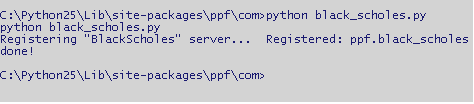
\includegraphics[scale=0.5]{img/register_server.PNG}
\caption{Registering the PPF Black-Scholes COM server.}
\end{figure}

Before we present an automation client that exercises the
functionality provided by our \verb|BlackScholes| component, we'll
quickly cover the definition of the \verb|OptionPrice| function. As
noted earlier, it's a simple wrapper around the
\verb|ppf.core.black_scholes| function. One important responsibility
of the wrapper is to trap any Python exceptions that may result from
the call to the \verb|ppf.core.black_scholes| function and translate
them into\\ \verb|win32.com.server.exception.COMException| exception
objects. The Python COM framework takes charge of phrasing such
exceptions in terms the calling environment (automation clients,) can
deal with. This is important since such environments will in general
know nothing about how to deal with raw Python exceptions (in fact,
the code
\begin{verbatim}
     raise COMException(
          desc="ppf error : \""+str(e)+"\"", scode=0x80040201)
\end{verbatim}
is creating a \verb|COMException| with a custom error
code. This works around a VB6 bug(?) and makes sure the text of the
the exception, detailing the \verb|ppf| error, is made available to
the calling client.)

\subsection{VBS client}

COM is all about getting objects in different languages talking to
each other. We'll put that to the test right now by implementing a
client of the \verb|BlackScholes| server from the preceding section
in Microsoft VBScript that is intended to be executed under the
Microsoft Windows Scripting Host environment offered by the command
line interpreter \verb|cscript.exe|. The code can be found in the
`example' directory of the code accompanying the book in the file
`test\_black\_scholes.vbs'.
\begin{verbatim}
On Error Resume Next

Dim Pricer : Set Pricer = CreateObject("ppf.black_scholes")
Dim spot: spot = 42.
Dim strike: strike = 40.
Dim r: r = 0.1
Dim sig: sig = 0.2
Dim T: T= 0.5
Dim european_call: european_call = 1

Dim price : price = Pricer.OptionPrice(spot, strike, r, sig, T, european_call)

If Err.Number <> 0 Then
  WScript.Echo "Automation error : " & vbCr & Err.Number & _
               " (" & Hex(Err.Number) & ")" & vbCr & Err.Description
  Err.Clear
Else
  WScript.Echo price
End If

Set Pricer = Nothing
\end{verbatim}
Figure \ref{fig:invoke-black-scholes-from-vbs} shows the result of
executing the client script.
\begin{figure}
\centering
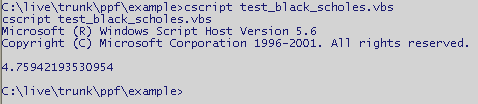
\includegraphics[scale=0.5]{img/black_scholes_vbs_client.PNG}
\caption{Invoking the PPF Black-Scholes function from VBScript.}
\label{fig:invoke-black-scholes-from-vbs}
\end{figure}

\subsection{VBA client}

The following Microsoft Excel VBA code implements a Black-Scholes
client suitable for use in Microsoft Excel. Figure
\ref{fig:invoke-black-scholes-from-vba} shows an example session
exercising the client on an Excel worksheet.
\begin{verbatim}
Public Function PPF_BlackScholes( _
   Spot As Double, _
   Strike As Double, _
   Rate As Double, _
   Vol As Double, _
   T As Double, _
   CallPut As Double) As Variant
  On Error Resume Next
  Dim Pricer As Object: Set Pricer = CreateObject("ppf.black_scholes")
  PPF_BlackScholes = Pricer.OptionPrice(Spot, Strike, Rate, Vol, T, CallPut)
  If Err.Number <> 0 Then
    PPF_BlackScholes = "#err: " & Err.Description
    Err.Clear
  End If
  Set Pricer = Nothing
End Function
\end{verbatim}
\begin{figure}
\centering
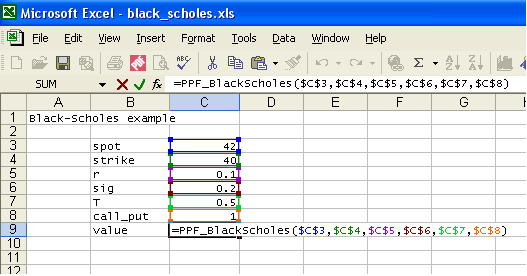
\includegraphics[scale=0.5]{img/black_scholes.PNG}
\caption{Invoking the PPF Black-Scholes function from Microsoft Excel.}
\label{fig:invoke-black-scholes-from-vba}
\end{figure}

\section{Numerical Pricing with PPF in Excel}

Armed with the understanding of the basic principles of publishing
Python COM components from the preceding section, we now consider how
we can assemble such components into a broader example to provide
numerical pricing capabilities using PPF in Excel. Specifically, our
goal will be to enable Bermudan swaption pricing on a Hull-White
lattice.

\subsection{Common utilities}

Before going on, we will find in implementing the COM servers for this
example some code that is common amongst all the servers that it is
helpful to factor out (to aid clarity and reduce unnecessary code
repetition). The simple utilities presented here all reside in the the
\verb|ppf.com.utils| module.

\subsubsection{Date conversion}

The \verb|to_ppf_date| function converts a Win32 COM date into a
\verb|ppf.date_time.date| representation. It is frequently used at the
boundary between the COM servers and `pure' \verb|ppf| Python:
\begin{verbatim}
def to_ppf_date(t):
  import ppf.date_time
  return ppf.date_time.date(t.year, t.month, t.day)
\end{verbatim}

\subsubsection{COM class registration}

Although no great saving as stated, the \verb|register_com_class|
function does abstract away the details of COM server registration and
provides a convenient hook for associating other actions at the time
of COM class registration in the future.
\begin{verbatim}
def register_com_class(classobj):
  import win32com.server.register
  win32com.server.register.UseCommandLine(classobj)
\end{verbatim}

\subsubsection{COM exceptions}

A simple function abstracting away the details of raising \\
\verb|win32.server.exception.COMException|s.
\begin{verbatim}
def raise_com_exception(e):
  from win32com.server.exception import COMException
  raise COMException(
    desc="ppf error : \""+str(e)+"\"", scode=0x80040201)
\end{verbatim}

\subsubsection{Symbol retrieval}

We will see an application for the following function in the next
section. It is a function that works as follows: given the name of a
module (`\verb|module|'), the name of a class object
(`\verb|server|'), the name of a symbol (`\verb|tag|') and the name of
a dictionary (`\verb|what|'), the function attempts to retrieve the
value associated with the key `\verb|tag|' from the dictionary
\verb|module.server._what| raising an exception in the event that the
operation cannot be fulfilled.
\begin{verbatim}
def retrieve(module, server, tag, what):
  exec("from %s import %s "% (module, server))
  table=eval(server+"._"+what)
  if not table.has_key(tag):
    raise RuntimeError, "\""+tag+"\" not found"
  return table[tag]
\end{verbatim}

\subsection{Market Server}\label{subsec:market-server}

The first step in numerical pricing is a need to construct the market
data environment in which to price. In this section we introduce the
\verb|class MarketServer| COM component the code for which resides in
the \verb|ppf.com.market_server| module. The responsibility of this
component is to wrap the services provided by the
\verb|ppf.market.enviroment| module (the \verb|ppf.market| package was
covered in chapter \ref{ch:market-curves-surfaces}). Here's the code:
\begin{verbatim}
import ppf.market
import utils

class MarketServer(object):
  _reg_progid_ = "ppf.market"
  _reg_clsid_ = "{CAFAEEDF-E876-4DD6-9B6F-7038EDA25BCD}"
  _public_methods_ = \
  [
      "CreateEnvironment"
             , "AddCurve"
           , "AddSurface"
          , "AddConstant"
  ]
  _environments = {}

  retrieve = staticmethod(
       lambda tag, which :
         utils.retrieve('market_server', 'MarketServer', tag, which))

  def CreateEnvironment(self, tag, t):
     try:
       MarketServer._environments[tag] = \
          ppf.market.environment(utils.to_ppf_date(t))
       return tag
     except RuntimeError, e: utils.raise_com_exception(e)

  def AddCurve(self, tag, name, curve, interp):
    try:
      import ppf.math.interpolation
      interp = eval("ppf.math.interpolation."+interp)
      times, factors = [x[1] for x in curve[1:]],[x[2] for x in curve[1:]]
      MarketServer.retrieve(tag, 'environments').add_curve(
          str(name), ppf.market.curve(times, factors, interp))
    except RuntimeError, e: utils.raise_com_exception(e)

  def AddConstant(self, tag, name, value):
    try:
      MarketServer.retrieve(tag, 'environments').add_constant(
        str(name), value)
    except RuntimeError, e: utils.raise_com_exception(e)

  def AddSurface(self, tag, name, expiries, tenors, values):
    try:
      import numpy
      exp, ten = expiries[1:], tenors[1:]
      surface = [x[1:] for x in values[1:]]
      MarketServer.retrieve(tag,'environments').add_surface(
        str(name), ppf.market.surface(exp, ten, numpy.array(surface)))
    except RuntimeError, e: utils.raise_com_exception(e)

if __name__ == "__main__": utils.register_com_class(MarketServer)
\end{verbatim}

To begin our explanation of the above code, note the existence of the
class `static' member \verb|_environments|. This data member will be
used to contain \verb|class environment| instances (from the
\verb|ppf.market.environment| module), each of which will be
associated with a user provided `name'. Access to the
\verb|_environments| member is given by the class static method
\verb|retrieve| implemented easily using the
\verb|ppf.com.utils.retrieve| function, the Python built in
\verb|staticmethod| function and partial function application achieved
with a $\lambda$ expression (isn't Python wonderfully
expressive?). The \verb|retrieve| method is not part of the COM
interface of \verb|class MarketServer|, it is there for interaction
between the servers, on the Python side. The use of a class static
data member to hold the environments makes the design of 
\verb|class MarketServer| an example of a `mono-state' pattern; all
instances share the same state and are therefore equivalent. Excepting
the \verb|retrieve| function, the remaining methods of \\
\verb|class MarketServer| satisfy its COM interface.

\subsubsection{CreateEnvironment}
The \verb|CreateEnvironment| method takes a user supplied name for an
environment, a COM date (the pricing date for the market), creates an
empty \\ 
\verb|class environment| instance, stores it in the
\verb|_environments| dictionary for later retrieval and simply returns
the user provided name for the environment to indicate success. Should
the operation fail for any reason, the Python exception is caught and
a COM exception raised by means of the \\
\verb|ppf.com.utils.raise_com_exception| function. This exception
handling idiom at the Python/COM boundary (explained in section
\ref{sec:black-scholes-com-server} ) will be the same for every COM
interface method and we will refrain from remarking on it again going
forward.

\subsubsection{AddCurve}\label{subsec:AddCurve}
The \verb|AddCurve| function `injects' a user-supplied curve into the
named market environment. We will look at this function in a little
more detail:
\begin{verbatim}
  def AddCurve(self, tag, name, curve, interp):
    try:
      import ppf.math.interpolation
      interp = eval("ppf.math.interpolation."+interp)
      times, factors = [x[1] for x in curve[1:]],[x[2] for x in curve[1:]]
      MarketServer.retrieve(tag, 'environments').add_curve(
          str(name), ppf.market.curve(times, factors, interp))
    except RuntimeError, e: utils.raise_com_exception(e)
\end{verbatim}
The \verb|tag| parameter indicates the name of the environment in
which the curve is to be stored. The \verb|interp| parameter is a
\verb|ppf.math.interpolation| class name: one of \verb|linear|,
\verb|loglinear|, \verb|linear_on_zero|, \verb|linear_on_variance| or
\verb|cubic_spline|. The assignment
\begin{verbatim}
  interp = eval("ppf.math.interpolation."+interp)
\end{verbatim} attempts to retrieve the \verb|ppf.math.interpolation|
module class object corresponding to the given string. 

The statement,
\begin{verbatim}
  times, factors = [x[1] for x in curve[1:]],[x[2] for x in curve[1:]]
\end{verbatim} might at first seem a little cryptic. From the COM client's
perspective, the \verb|curve| is provided as a two-column array. As we
will see later, VBA code to construct the curve would read something like:
\begin{verbatim}
  Dim V As Variant
  Dim N As Integer: N = Curve.Rows.Count
  ReDim V(N, 2)
  Dim I As Integer
  For I = 1 To N
    V(I, 1) = Curve(I, 1).Value
    V(I, 2) = Curve(I, 2).Value
  Next I
\end{verbatim}
On the server side however, what arrives in Python from the PythonCOM
framework will actually be a 3-column array, say something like the
following example:
\begin{verbatim}
((None, None, None),
 (None, 0.0, 1.0),
 (None, 0.5, 0.97530991202833262),
 (None, 1.0, 0.95122942450071402),
 (None, 1.5, 0.92774348632855286),
 (None, 2.0, 0.90483741803595952),
 (None, 3.0, 0.86070797642505781),
 (None, 4.0, 0.81873075307798182),
 (None, 5.0, 0.77880078307140488),
 (None, 6.0, 0.74081822068171788),
 (None, 7.0, 0.70468808971871344),
 (None, 8.0, 0.67032004603563933),
 (None, 9.0, 0.63762815162177333),
 (None, 10.0, 0.60653065971263342),
 (None, 11.0, 0.57694981038048665))
\end{verbatim} so, in order to get the required data out of the
incoming curve it's necessary to `skip' the first row, and the first
column. 

Assuming the preceding operations all succeed, 
\begin{verbatim}
      MarketServer.retrieve(tag, 'environments').add_curve(
          str(name), ppf.market.curve(times, factors, interp))
\end{verbatim}
retrieves the named environment from \verb|MarketServer| class object
by means of its static \verb|retrieve| function, a new
\verb|ppf.market.curve| instance is created, and is installed into the
environment. One slight but important detail should be mentioned; the
presence of invoking the built-in \verb|str| function on the
\verb|name| argument in the call to the \verb|class environment|
\verb|add_curve| function. The reason for this is that the \verb|name|
argument is a \emph{unicode} string, whereas \verb|ppf| traffics in
regular ASCII strings. Invoking \verb|str| handles the necessary
``narrowing'' conversion.

\subsubsection{AddConstant}

The explanation of \verb|AddCurve| above was necessarily lengthy; a
great deal of detail was covered. The \verb|AddConstant| function
which injects a named constant into a given enviroment,
\begin{verbatim}
  def AddConstant(self, tag, name, value):
    try:
      MarketServer.retrieve(tag, 'environments').add_constant(
        str(name), value)
    except RuntimeError, e: utils.raise_com_exception(e)
\end{verbatim}
should now be readily understandable.

\subsubsection{AddSurface}

The \verb|AddSurface| function uses all the tricks uncovered in the
explanation of the \verb|AddCurve| method (see sub-section
\ref{subsec:AddCurve}):
\begin{verbatim}
  def AddSurface(self, tag, name, expiries, tenors, values):
    try:
      import numpy
      exp, ten = expiries[1:], tenors[1:]
      surface = [x[1:] for x in values[1:]]
      MarketServer.retrieve(tag,'environments').add_surface(
        str(name), ppf.market.surface(exp, ten, numpy.array(surface)))
    except RuntimeError, e: utils.raise_com_exception(e)
\end{verbatim}
In this function, \verb|exp| is an array of $M$ expiries (in years),
\verb|tenors| an array $N$ tenors (in days) and \verb|surface| the
surface data as an $M \times N$ array. Figure
\ref{fig:add-surface-to-market} shows how the data for the surface
might be arranged in an Excel worksheet.
\begin{figure} \centering
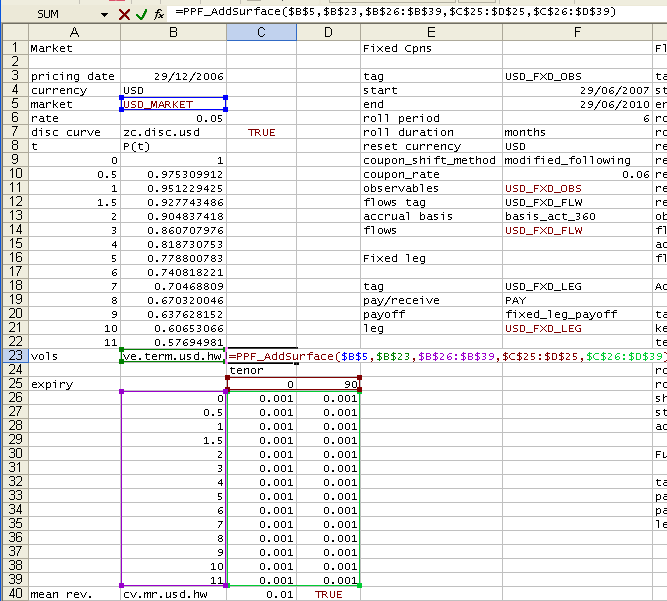
\includegraphics[scale=0.5]{img/market_server.PNG}
\caption{Adding a surface to a market environment.}
\label{fig:add-surface-to-market}
\end{figure}

\subsubsection{Market VBA client}

The foregoing section detailed the workings of the COM object known by
the ProgID \emph{`ppf.market'}. What remains is client code on the Excel
VBA side to exercise it's functionality.

It seems fair to assume that readers with interest in this chapter are
familiar with Excel and Excel VBA so we will make little comment on the
example VBA code presented here.

\subsubsection{PPF\_CreateMarketEnvironment}

This function calls out to the \verb|class MarketServer|
\verb|CreateEnvironment| method to construct and register an empty
\verb|ppf.market.environment.environment| instance.
\begin{verbatim}
Public Function _
PPF_CreateMarketEnvironment( _
    Tag As String _
  , T As Date) As String
'Create a ppf market data environment
'
On Error Resume Next
  Dim MarketServer As Object
  Set MarketServer = CreateObject("ppf.market")
  PPF_CreateMarketEnvironment = MarketServer.CreateEnvironment(Tag, T)
  If Err.Number <> 0 Then
    PPF_CreateMarketEnvironment = "#err: " & Err.Description
  End If
  Set MarketServer = Nothing
End Function
\end{verbatim}

\subsubsection{PPF\_AddCurve}

This function calls out to the \verb|class MarketServer|
\verb|AddCurve| method to register a user defined curve in a
previously constructed environment.
\begin{verbatim}
Public Function _
PPF_AddCurve( _
    Market As String _
  , Name As String _
  , Curve As Variant _
  , Interp As String) As Variant
  'Add a curve to a ppf market data environment
  '
  On Error Resume Next
  Dim MarketServer As Object
  Dim N As Integer: N = Curve.Rows.Count
  If Curve.Columns.Count <> 2 Then
    PPF_AddCurve = "#err: invalid argument"
    Exit Function
  End If
  Dim V As Variant
  ReDim V(N, 2)
  Dim I As Integer
  For I = 1 To N
    V(I, 1) = Curve(I, 1).Value
    V(I, 2) = Curve(I, 2).Value
  Next I
  Set MarketServer = CreateObject("ppf.market")
  Call MarketServer.AddCurve(Market, Name, V, Interp)
  If Err.Number <> 0 Then
    PPF_AddCurve = "#err: " & Err.Description
  Else
    PPF_AddCurve = True
  End If
  Set MarketServer = Nothing
End Function
\end{verbatim}

\subsubsection{PPF\_AddConstant}
This function calls out to the \verb|class MarketServer|
\verb|AddConstant| method to register a user constant in a previously
constructed environment.
\begin{verbatim}
Public Function _
PPF_AddConstant( _
    Market As String _
  , Name As String _
  , Value As Double) As Variant
  'Add a constant to a ppf market data environment
  '
  On Error Resume Next
  Dim MarketServer As Object
  Set MarketServer = CreateObject("ppf.market")
  Call MarketServer.AddConstant(Market, Name, Value)
  If Err.Number <> 0 Then
    PPF_AddConstant = "#err: " & Err.Description
  Else
    PPF_AddConstant = True
  End If
  Set MarketServer = Nothing
End Function
\end{verbatim}

\subsubsection{PPF\_AddSurface}
This function calls out to the \verb|class MarketServer|
\verb|AddSurface| method to register a user defined surface in a previously
constructed environment.
\begin{verbatim}
Public Function _
PPF_AddSurface( _
    Market As String _
  , Name As String _
  , Expiries As Variant _
  , Tenors As Variant _
  , Surface As Variant)
  'Add a surface to a ppf market data environment
  '
  On Error Resume Next
  Dim NumExp As Integer: NumExp = Expiries.Rows.Count
  Dim NumTen As Integer: NumTen = Tenors.Columns.Count
  If Surface.Rows.Count <> NumExp Or _
     Surface.Columns.Count <> NumTen Then
    PPF_AddSurface = "#err: invalid argument"
  End If
  Dim Exp As Variant
  ReDim Exp(NumExp)
  Dim I, J As Integer
  For I = 1 To NumExp
    Exp(I) = Expiries(I).Value
  Next I
  Dim Ten As Variant
  ReDim Ten(NumTen)
  For I = 1 To NumTen
    Ten(I) = Tenors(1, I).Value
  Next I
  Dim Values As Variant
  ReDim Values(NumExp, NumTen)
  For I = 1 To NumExp
    For J = 1 To NumTen
        Values(I, J) = Surface(I, J).Value
    Next J
  Next I
  Dim MarketServer As Object
  Set MarketServer = CreateObject("ppf.market")
  Call MarketServer.AddSurface(Market, Name, Exp, Ten, Values)
  If Err.Number <> 0 Then
    PPF_AddSurface = "#err : " & Err.Description
  Else
    PPF_AddSurface = True
  End If
  Set MarketServer = Nothing
End Function
\end{verbatim}

\subsection{Trade Server}

Having constructed a market, the next step in numerical pricing is to
describe the trade to be priced. This section outlines the 
\verb|class TradeServer| COM component. The code in this section can be found in
the \verb|ppf.com.trade_server| module. Instances of this type wrap
the services offered up by the \verb|ppf.core| module, specifically,
those relating to the \verb|ppf| trade data model (this functionality
was explained in chapter \ref{ch:data-model}). Here we go with the code:
\begin{verbatim}
import ppf.core
import ppf.pricer.payoffs
import ppf.date_time
import utils

class TradeServer(object):
  _reg_progid_ = "ppf.trade"
  _reg_clsid_ = "{E33DA322-B011-4FE9-8AB9-87A964EDD046}"
  _public_methods_ = \
   [
        "GenerateFixedCouponObservables"
            , "GenerateLiborObservables"
                       , "GenerateFlows"
               , "GenerateAdjuvantTable"
            , "GenerateExerciseSchedule"
                           , "CreateLeg"
                         , "CreateTrade"
  ]
  _observables = {}
  _flows       = {}
  _adjuvants   = {}
  _legs        = {}
  _exercises   = {}
  _trades      = {}

  retrieve = staticmethod(
       lambda tag, which :
         utils.retrieve('trade_server', 'TradeServer', tag, which))

  def GenerateFixedCouponObservables(
      self
      , tag
      , start
      , end
      , roll_period
      , roll_duration
      , reset_currency
      , coupon_shift_method
      , coupon_rate):
    try:
      observables = \
       ppf.core.generate_fixed_coupon_observables(
            start=utils.to_ppf_date(start)
          , end=utils.to_ppf_date(end)
          , roll_period=roll_period
          , roll_duration=eval("ppf.date_time."+roll_duration)
          , reset_currency=reset_currency
          , coupon_shift_method=
              eval("ppf.date_time.shift_convention."+coupon_shift_method)
          , coupon_rate=coupon_rate)
      TradeServer._observables[tag] = observables
      return tag
    except RuntimeError, e: utils.raise_com_exception(e)

  def GenerateLiborObservables(
      self
      , tag
      , start
      , end
      , roll_period
      , roll_duration
      , reset_period
      , reset_duration
      , reset_currency
      , reset_basis
      , reset_shift_method):
    try:
      observables = \
        ppf.core.generate_libor_observables(
            start=utils.to_ppf_date(start)
          , end=utils.to_ppf_date(end)
          , roll_period=roll_period
          , roll_duration = eval("ppf.date_time."+roll_duration)
          , reset_period = reset_period
          , reset_duration = eval("ppf.date_time."+reset_duration)
          , tenor_period = reset_period
          , tenor_duration = eval("ppf.date_time."+reset_duration)
          , reset_currency=reset_currency
          , reset_basis = eval("ppf.date_time."+reset_basis)
          , reset_shift_method=eval( \
             "ppf.date_time.shift_convention."+reset_shift_method)
          , reset_lag = 0)
      TradeServer._observables[tag] = observables
      return tag
    except RuntimeError, e: utils.raise_com_exception(e)

  def GenerateFlows(
      self
      , tag
      , start
      , end
      , period
      , duration
      , pay_currency
      , pay_shift_method
      , accrual_basis
      , observables):
    try:
      flows = ppf.core.generate_flows(
          start=utils.to_ppf_date(start)
          , end=utils.to_ppf_date(end)
          , duration=eval("ppf.date_time."+duration)
          , period=period
          , pay_shift_method=eval(\
              "ppf.date_time.shift_convention."+pay_shift_method)
          , pay_currency=pay_currency
          , accrual_basis=eval("ppf.date_time."+accrual_basis)
          , observables=TradeServer.retrieve(observables, 'observables'))
      TradeServer._flows[tag] = flows
      return tag
    except RuntimeError, e: utils.raise_com_exception(e)

  def GenerateAdjuvantTable(
      self
      , tag
      , items
      , tens
      , vals
      , start
      , roll_period
      , roll_duration
      , shift_method):
    try:
      import numpy
      adjuvants = \
         ppf.core.generate_adjuvant_table(
              items[1:]
            , [int(t) for t in tens[1:]]
            , numpy.array([x[1:len(vals[0])] for x in vals[1:]])
            , utils.to_ppf_date(start)
            , rol_period=roll_period
            , roll_duration=eval("ppf.date_time."+roll_duration)
            , shift_method=eval(\
                 "ppf.date_time.shift_convention."+shift_method))
      TradeServer._adjuvants[tag] = adjuvants
      return tag
    except RuntimeError, e: utils.raise_com_exception(e)

  def GenerateExerciseSchedule(
      self
      , tag
      , start
      , end
      , period
      , duration
      , shift_method):
    try:
      sched = \
        ppf.core.generate_exercise_table(
            start = utils.to_ppf_date(start)
          , end = utils.to_ppf_date(end)
          , period = period
          , duration = eval("ppf.date_time."+duration)
          , shift_method = eval("ppf.date_time.shift_convention."+shift_method))
      TradeServer._exercises[tag] = sched
      return tag
    except RuntimeError, e:
      utils.raise_com_exception(e)
    
  def CreateLeg(
    self
    , tag
    , flows
    , pay_or_receive
    , adjuvant_table
    , payoff):
    try:
      adjuvants = None
      if adjuvant_table:
        adjuvants = TradeServer.retrieve(adjuvant_table, 'adjuvants')
      leg = \
          ppf.core.leg(
             TradeServer.retrieve(flows, 'flows')
             , eval("ppf.core."+pay_or_receive)
             , adjuvants
             , eval("ppf.pricer.payoffs."+payoff)())
      TradeServer._legs[tag] = leg
      return tag
    except RuntimeError, e: utils.raise_com_exception(e)

  def CreateTrade(
    self
    , tag
    , legs
    , exercise_sched
    , exercise_type):
    try:
      tl = [TradeServer.retrieve(l, 'legs') for l in legs[1:]]
      if exercise_sched:
        exercises = TradeServer.retrieve(exercise_sched, 'exercises')
        if not exercise_type:
          raise RuntimeError, "missing exercise type"
        call_cancel = eval("ppf.core.exercise_type."+exercise_type)
        trade = ppf.core.trade(tl, (exercises, call_cancel))
      else:
        trade = ppf.core.trade(tl, None)
      TradeServer._trades[tag] = trade
      return tag
    except RuntimeError, e: utils.raise_com_exception(e)
    
if __name__ == "__main__": utils.register_com_class(TradeServer)
\end{verbatim}

Sub-section \ref{subsec:market-server} covers the details of what
needs to be known to `technically' understand the above code so this
section need not be so detailed from that perspective.

As is the case for \verb|class MarketServer|, the \verb|class TradeServer|
implementation follows a `mono-state' idiom. Unlike, 
\verb|class MarketServer|, however, \verb|class TradeServer| maintains
multiple dictionaries in its class object state
\begin{verbatim}
  _observables = {} #observable collections
  _flows       = {} #flow collections
  _adjuvants   = {} #adjuvant tables
  _legs        = {} #trade legs
  _exercises   = {} #exercise schedules
  _trades      = {} #trades
\end{verbatim}
As for \verb|class MarketServer|, \verb|class TradeServer| offers a
static method for inter-module retrieval of data from these
dictionaries. 

As for the COM interface, \verb|GenerateFixedCouponObservables| rolls
out strips of fixed coupons, whereas
\verb|GenerateLiborCouponObservables| rolls out strips of LIBORs (it's
left as an exercise to the reader to write the function that rolls out
strips of swap rate observables). \verb|GenerateFlows| rolls out flows
with observable collections folded in. \verb|GenerateAdjuvantTable|
and \\
\verb|GenerateExerciseSchedule| provide the means of constructing
adjuvant tables (refer to section \ref{sec:adjuvant-tables}) and
exercise schedules respectively. Finally, \verb|CreateLeg| assembles a
flow collection, a user provided payoff string and potentially an
adjuvant table into a trade leg (the payoff string needs to map to a
class name in the \verb|ppf.pricer.payoffs| module
such as, \verb|fixed_leg_payoff|, \verb|float_leg_payoff| for
example). Finally, legs and perhaps an associated exercise schedule
can be aggregated into trades with the \verb|CreateTrade| method. Figure
\ref{fig:create-trade} shows how the data for describing a Bermudan
swaption might be laid out in an Excel worksheet.
\begin{figure} 
\centering
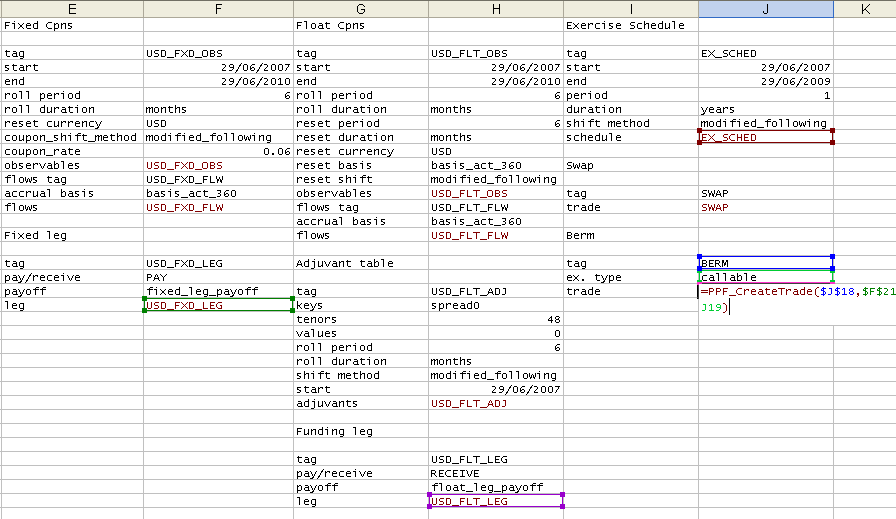
\includegraphics[scale=0.4]{img/trade_server.PNG}
\caption{Creating a Bermudan swaption.}
\label{fig:create-trade}
\end{figure}

\subsubsection{Trade VBA client}

Here is example client code for interfacing to the
\emph{`ppf.trade'} COM object.

\subsubsection{PPF\_GenerateFixedCouponObservables}

This function calls out to the \verb|class TradeServer|
\verb|GenerateFixedCouponObservables| method to create and register
observables to underly a fixed trade leg.

\begin{verbatim}
Public Function _
PPF_GenerateFixedCouponObservables( _
    Tag As String _
  , Begin As Date _
  , Finish As Date _
  , Period As Integer _
  , Duration As String _
  , Ccy As String _
  , Shift As String _
  , Rate As Double) As String
  'Generate a ppf fixed coupon observable sequence
  '
  On Error Resume Next
  Dim TradeServer As Object
  Set TradeServer = CreateObject("ppf.trade")
  PPF_GenerateFixedCouponObservables = _
    TradeServer.GenerateFixedCouponObservables( _
        Tag _
      , Begin _
      , Finish _
      , Period _
      , Duration _
      , Ccy _
      , Shift _
      , Rate)
  If Err.Number <> 0 Then
    PPF_GenerateFixedCouponObservables = "#err : " & Err.Description
  End If
  Set TradeServer = Nothing
End Function
\end{verbatim}

\subsubsection{PPF\_GenerateLiborObservables}

This function calls out to the \verb|class TradeServer|
\verb|GenerateLiborObservables| method to create and register the
observables to underly a funding trade leg.
\begin{verbatim}
Public Function _
PPF_GenerateLiborObservables( _
    Tag As String _
  , Begin As Date _
  , Finish As Date _
  , RollPeriod As Integer _
  , RollDuration As String _
  , ResetPeriod As Integer _
  , ResetDuration As String _
  , ResetCcy As String _
  , ResetBasis As String _
  , ResetShift As String) As String
  'Generate a ppf libor observable sequence
  '
  On Error Resume Next
  Dim TradeServer As Object
  Set TradeServer = CreateObject("ppf.trade")
  PPF_GenerateLiborObservables = _
    TradeServer.GenerateLiborObservables( _
        Tag _
      , Begin _
      , Finish _
      , RollPeriod _
      , RollDuration _
      , ResetPeriod _
      , ResetDuration _
      , ResetCcy _
      , ResetBasis _
      , ResetShift)
  If Err.Number <> 0 Then
    PPF_GenerateLiborObservables = "#err : " & Err.Description
  End If
  Set TradeServer = Nothing
End Function
\end{verbatim}

\subsubsection{PPF\_GenerateAdjuvantTable}

This function calls out to the \verb|class TradeServer|
\verb|GenerateAdjuvantTable| method to build and register an
adjuvant table.
\begin{verbatim}
Public Function _
PPF_GenerateAdjuvantTable( _
    Tag As String _
  , Items As Variant _
  , Tenors As Variant _
  , Values As Variant _
  , Start As Date _
  , RollPeriod As Integer _
  , RollDuration As String _
  , ShiftConv As String) As String
  'Generate a ppf adjuvant table
  '
  On Error Resume Next
  Dim TradeServer As Object
  Set TradeServer = CreateObject("ppf.trade")
  Dim K As Integer
  K = Items.Rows.Count
  If Items.Columns.Count <> 1 Then
   PPF_GenerateAdjuvantTable = "#err : " & "invalid argument"
   Exit Function
  End If
  Dim Keys As Variant
  ReDim Keys(K)
  Dim I, J As Integer
  For I = 1 To K
    Keys(I) = Items(I).Value
  Next I
  Dim M, N As Integer
  M = Values.Rows.Count
  N = Values.Columns.Count
  If M <> K Then
   PPF_GenerateAdjuvantTable = "#err : " & "invalid argument"
   Exit Function
  End If
  Dim Vals As Variant
  ReDim Vals(M, N)
  For I = 1 To M
    For J = 1 To N
        Vals(I, J) = Values(I, J).Value
    Next J
  Next I
  If Tenors.Rows.Count > 1 Or Tenors.Columns.Count <> N Then
   PPF_GenerateAdjuvantTable = "#err : " & "invalid argument"
   Exit Function
  End If
  Dim Tens As Variant
  ReDim Tens(N)
  For J = 1 To N
    Tens(J) = Tenors(J).Value
  Next J
  PPF_GenerateAdjuvantTable = _
    TradeServer.GenerateAdjuvantTable( _
        Tag _
      , Keys _
      , Tens _
      , Vals _
      , Start _
      , RollPeriod _
      , RollDuration _
      , ShiftConv)
  If Err.Number <> 0 Then
    PPF_GenerateAdjuvantTable = "#err : " & Err.Description
  End If
  Set TradeServer = Nothing

End Function
\end{verbatim}

\subsubsection{PPF\_GenerateFlows}

This function calls out to the \verb|class TradeServer|
\verb|GenerateFlows| method to create and register a flow collection.
\begin{verbatim}
Public Function _
PPF_GenerateFlows( _
    Tag As String _
  , Begin As Date _
  , Finish As Date _
  , Period As Integer _
  , Duration As String _
  , Ccy As String _
  , Shift As String _
  , Basis As String _
  , Observables As String) As String
  'Generate a ppf flow sequence
  '
  On Error Resume Next
  Dim TradeServer As Object
  Set TradeServer = CreateObject("ppf.trade")
  PPF_GenerateFlows = _
    TradeServer.GenerateFlows( _
        Tag _
      , Begin _
      , Finish _
      , Period _
      , Duration _
      , Ccy _
      , Shift _
      , Basis _
      , Observables)
  If Err.Number <> 0 Then
    PPF_GenerateFlows = "#err : " & Err.Description
  End If
  Set TradeServer = Nothing
End Function
\end{verbatim}

\subsubsection{PPF\_GenerateExerciseSchedule}

This function calls out to the \verb|class TradeServer|
\verb|GenerateExerciseSchedule| method to create and register an
exercise schedule.
\begin{verbatim}
Public Function _
PPF_GenerateExerciseSchedule( _
    Tag As String _
  , Begin As Date _
  , Finish As Date _
  , Period As Integer _
  , Duration As String _
  , Shift As String) As String
  'Generate a ppf exercise schedule
  '
  On Error Resume Next
  Dim TradeServer As Object
  Set TradeServer = CreateObject("ppf.trade")
  PPF_GenerateExerciseSchedule = _
    TradeServer.GenerateExerciseSchedule( _
        Tag _
      , Begin _
      , Finish _
      , Period _
      , Duration _
      , Shift)
  If Err.Number <> 0 Then
    PPF_GenerateExerciseSchedule = "#err : " & Err.Description
  End If
  Set TradeServer = Nothing
End Function
\end{verbatim}

\subsubsection{PPF\_CreateLeg}

This function calls out to the \verb|class TradeServer|
\verb|CreateLeg| function to create and register a trade leg.
\begin{verbatim}
Public Function _
PPF_CreateLeg( _
    Tag As String _
  , Flows As String _
  , PayOrReceive As String _
  , AdjuvantTable As Variant _
  , Payoff As String) As String
  'Create a ppf trade leg
  '
  On Error Resume Next
  Dim TradeServer As Object
  Set TradeServer = CreateObject("ppf.trade")
  If IsMissing(AdjuvantTable) Then
    PPF_CreateLeg = _
      TradeServer.CreateLeg( _
          Tag _
        , Flows _
        , PayOrReceive _
        , Nothing _
        , Payoff)
  Else
    PPF_CreateLeg = _
      TradeServer.CreateLeg( _
          Tag _
        , Flows _
        , PayOrReceive _
        , CStr(AdjuvantTable) _
        , Payoff)
  End If
  If Err.Number <> 0 Then
    PPF_CreateLeg = "#err : " & Err.Description
  End If
  Set TradeServer = Nothing

End Function
\end{verbatim}

\subsubsection{PPF\_CreateTrade}

This function calls out to the \verb|class TradeServer|
\verb|CreateTrade| method to create and register a trade.
\begin{verbatim}
Public Function _
PPF_CreateTrade( _
    Tag As String _
  , Leg1 As String _
  , Leg2 As String _
  , ExerciseSched As Variant _
  , ExerciseType As Variant) As String
  'Create a ppf trade
  '
  On Error Resume Next
  Dim TradeServer As Object
  Set TradeServer = CreateObject("ppf.trade")
  Dim Legs(2) As String
  Legs(1) = Leg1: Legs(2) = Leg2
  If IsMissing(ExerciseSched) Then
    PPF_CreateTrade = _
      TradeServer.CreateTrade( _
          Tag _
        , Legs _
        , Nothing _
        , Nothing)
  Else
    PPF_CreateTrade = _
      TradeServer.CreateTrade( _
          Tag _
        , Legs _
        , CStr(ExerciseSched) _
        , CStr(ExerciseType))
  End If
  If Err.Number <> 0 Then
    PPF_CreateTrade = "#err : " & Err.Description
  End If
  Set TradeServer = Nothing
End Function
\end{verbatim}

\subsection{Pricer Server}\label{subsec:pricer-server}

We are very close to achieving the goal as stated in the opening to
this section, that is, pricing Bermudans on a Hull-White lattice from
Excel.

The last component to consider is the \verb|class PricerServer| the
code for which can be found in the \verb|ppf.com.pricer_server|
module:
\begin{verbatim}
import ppf.model
import ppf.pricer
import utils

class PricerServer(object):
  _reg_progid_ = "ppf.pricer"
  _reg_clsid_ = "{08632905-0B63-45B5-B388-30C73CAE611C}"
  _public_methods_ = \
  [
      "CreateHullWhiteLatticePricer"
                    , "InvokePricer"
  ]
  _pricers = {}

  retrieve = staticmethod(
       lambda tag, which :
         utils.retrieve('pricer_server', 'PricerServer', tag, which))

  def CreateHullWhiteLatticePricer(
      self
      , tag
      , trade_id
      , env_id
      , num_states
      , num_std_dev):
    try:
      from trade_server import TradeServer
      from market_server import MarketServer
      trade = TradeServer.retrieve(trade_id, 'trades')
      env   = MarketServer.retrieve(env_id, 'environments')
      model_args = {"num states": num_states, "num std dev": num_std_dev} 
      factory = ppf.model.hull_white_lattice_model_factory()
      model = factory(trade, env, model_args)
      pricer = ppf.pricer.lattice_pricer(trade, model, env, None)
      PricerServer._pricers[tag] = pricer
      return tag
    except RuntimeError, e: ppf.com.utils.raise_com_exception(e)

  def InvokePricer(self, tag):
    try:
      return PricerServer.retrieve(tag, 'pricers').__call__()
    except RuntimeError, e: utils.raise_com_exception(e)

if __name__ == "__main__": utils.register_com_class(PricerServer)
\end{verbatim}
The explanations provided by the earlier sections should make the
above code self-explanatory rendering further comment unnecessary.
Figure \ref{fig:price-bermudan} shows an example session pricing a
Bermudan in an Excel session.
\begin{figure} \centering
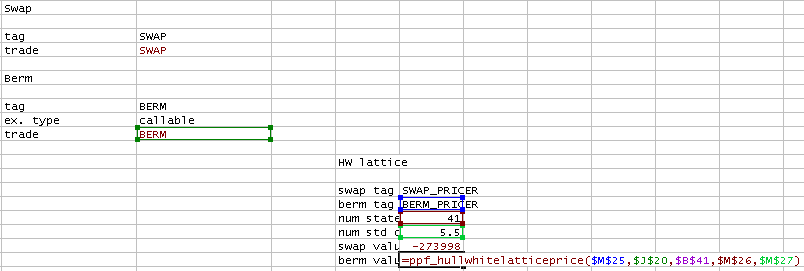
\includegraphics[scale=0.5]{img/pricer_server.PNG}
\caption{Pricing a berm.}
\label{fig:price-bermudan}
\end{figure}

\subsubsection{Pricer VBA client}

Here is the example client code for interfacing to the
\emph{`ppf.pricer'} COM object.

\subsubsection{PPF\_HullWhiteLatticePrice}

The function for obtaining the price of a trade via the Hull-White
model on a lattice.

\begin{verbatim}
Public Function _
PPF_HullWhiteLatticePrice( _
    Tag As String _
  , trade As String _
  , Env As String _
  , NumStates As Integer _
  , NumStdDevs As Double) As Variant
  'Price trade on a Hull-White lattice
  '
  On Error Resume Next
  Dim PricerServer As Object
  Set PricerServer = CreateObject("ppf.pricer")
  PPF_HullWhiteLatticePrice = _
    PricerServer.InvokePricer( _
      PricerServer.CreateHullWhiteLatticePricer( _
          Tag _
        , trade _
        , Env _
        , NumStates _
        , NumStdDevs))
  If Err.Number <> 0 Then
    PPF_HullWhiteLatticePrice = "#err : " & Err.Description
  End If
  Set PricerServer = Nothing
End Function
\end{verbatim}

  \begin{appendices}
    \chapter {Python} \label{appendix:python-tutorial}

In this appendix, we provide a whirlwind tour of the Python
programming language. It will in no way be exhaustive and is not
intended to negate the need for learning the language more
comprehensively using the many excellent resources available teaching
Python\footnote{A good place to start is the "Python
tutorial" available online at http://docs.python.org/tutorial/}. 
Nonetheless, it should be enough for a newcomer to the language to get
started.

\section{Python interpreter modes}

The Python interpreter can be executed in one of two modes,
`interactive' or `batch'. When run interactively in a shell or on
Windows, at a command prompt, the interpreter will wait for input from
the user and when sufficient input has been made for a statement to be
executed will execute that statement immediately and go back to
waiting for the next. In batch mode, a complete Python script stored
in a file is given to the interpreter and executed all in one go.

\subsection{Interactive mode}

To launch an interactive session with the interpreter, from your shell
or command prompt, issue the command \verb|python -i|. All being well,
the interpreter should then indicate its willingness to begin
processing statements by displaying its \emph{primary} prompt which
looks like a sideways chevron `\verb|>>>|'. On Windows, starting a
session might look something like this:
\begin{verbatim}
c:\Documents and Settings\PythonUser>python -i
python -i
ActivePython 2.5.1.1 (ActiveState Software Inc.) based on
Python 2.5.1 (r251:54863, May  1 2007, 17:47:05) [MSC v.1310 32 bit (Intel)] on win32
Type "help", "copyright", "credits" or "license" for more information.
>>> 
\end{verbatim}
When the interpreter has seen some part of a statement, but not
sufficiently enough to execute anything, the Python interpreter will
indicate that situation by displaying its \emph{secondary} prompt
which looks like `\verb|...|'.

\subsection{Batch mode}

To have the interpreter execute a complete Python script stored in a
file on disk, simply run the Python executable passing the name of the
script to be executed. For example, assuming the existence of a file
`hello\_world.py' (files containing Python script by convention have
a `.py' suffix), we might execute it like so:
\begin{verbatim}
c:\Documents and Settings\PythonUser>python hello_world.py
\end{verbatim}

\section{Basic Python}

\subsection{Simple expressions}

The Python interpreter can be used like a calculator to evaluate
numerical expressions:
\begin{verbatim}
>>> 1 + 2 + 3
6
\end{verbatim}
Number valued expressions in Python are of integer or floating point
type:
\begin{verbatim}
>>> 22/7
3
>>> 22/7.0
3.1428571428571428
>>> 
\end{verbatim}
String literal expressions are values too:
\begin{verbatim}
>>> "Hello world!"
'Hello world!'
>>> "Goodbye cruel " + "world."
'Goodbye cruel world.'
>>> 
\end{verbatim}
In the last example, we made use of the string concatenation operator
`\verb|+|' to concatenate two string literal expressions into one.

The value of an expression can be associated with a variable using the
\emph{assignment operator} denoted `\verb|=|':
\begin{verbatim}
>>> x = 1 + 2 + 3
\end{verbatim}
Doing so means the evaluation of the named expression can be referred
to again later:
\begin{verbatim}
>>> print x - 6
0
\end{verbatim}
Assigning a new expression to an existing variable causes the
expression the variable was associated with to be discarded and the
variable to become associated with the new expression instead:
\begin{verbatim}
>>> bar = "baz"
>>> print bar
baz
>>> bar = 42
>>> print bar
42
>>> 
\end{verbatim}
Comments are indicated by a `\verb|#|' and are ignored by the
interpreter:
\begin{verbatim}
>>> #this is a comment!
... 
>>> 
\end{verbatim}

\subsection{Built-in data types}

We have seen that natively Python supports integers, floating point
values and character strings. Python also natively provides incredibly
useful heterogeneous container types. The first of these is the
\emph{tuple}. A tuple is a fixed collection of values and can be
constructed using parentheses like so:
\begin{verbatim}
>>> t = (1, 2, "foo")
>>> print t
(1, 2, 'foo')
>>> \end{verbatim}
Naturally, tuples can contain values of any type including tuples:
\begin{verbatim}
>>> s = (t, t, (t,))
>>> print s
((1, 2, 'foo'), (1, 2, 'foo'), ((1, 2, 'foo'),))
>>> 
\end{verbatim}
The value at the $i$-th position of a tuple can be retrieved like this:
\begin{verbatim}
>>> print t[0]
1
>>> print t[1]
2
>>> print t[2]
foo
>>> print t[3] #uh-oh...
Traceback (most recent call last):
  File "<stdin>", line 1, in <module>
IndexError: tuple index out of range
>>> 
\end{verbatim}
Tuples can be used to assign to multiple values very concisely:
\begin{verbatim}
>>> x,y,z=t
>>> print "%d,%d,%s" % (x, y, z)
1,2,foo
\end{verbatim}
Tuples are immutable which means a tuple value may not be modified:
\begin{verbatim}
>>> t[0]=10
Traceback (most recent call last):
  File "<stdin>", line 1, in <module>
TypeError: 'tuple' object does not support item assignment
>>> 
\end{verbatim}
In fact, integers, floats, strings and tuples are all immutable types.

When a mutable sequence is needed, Python steps in with its
\emph{list} type. Lists are created using square brackets like this:
\begin{verbatim}
>>> l = [1, 1.0, "one"]
>>> print l
[1, 1.0, 'one']
>>> 
\end{verbatim}
Lists contain values of any type (built-in or user-defined) including
of course, tuples and lists.
\begin{verbatim}
>>> m = [l, t]
>>> print m
[[1, 1.0, 'one'], (1, 2, 'foo')]
>>> 
\end{verbatim}
Lists as mentioned are a mutable type:
\begin{verbatim}
>>> l[0], l[1], l[2] = (2, 2.0, 'two')
>>> print l
[2, 2.0, 'two']
>>> 
\end{verbatim}
Be careful! Because lists are not immutable one needs to be mindful of
side-effects resulting from aliasing:
\begin{verbatim}
>>> ll = l
>>> ll[0] = 3
>>> print l
[3, 2.0, 'two']
>>> 
\end{verbatim}
Do you see what's happened there? The value referred to by \verb|l|
was modified through an alias \verb|ll|. 

Now, Python has very powerful constructs for creating lists termed
\emph{list comprehensions}:
\begin{verbatim}
>>> u = [i for i in range(10)]
>>> print u
[0, 1, 2, 3, 4, 5, 6, 7, 8, 9]
>>> v = [i*i for i in u]
>>> print v
[0, 1, 4, 9, 16, 25, 36, 49, 64, 81]
>>> print [x for x in v if x > 25]
[36, 49, 64, 81]
\end{verbatim}
List comprehensions are very much worth finding out about as early as
possible.

Data structures commonly known as \emph{associated arrays} in other
programming languages are termed \emph{dictionaries} in Python. They
are arrays accessed by \emph{keys} where each key is associated with a
value. An empty dictionary is denoted `\verb|{}|':
\begin{verbatim}
>>> d = {}
>>> print d
{}
\end{verbatim}
A non-empty dictionary can be created by passing a sequence of
key-value pairs like so:
\begin{verbatim}
>>> d = {"1":1, "2":2, "3":3}
>>> print d
{'1': 1, '3': 3, '2': 2}
\end{verbatim}
Naturally, dictionary values may be of any type including lists and
tuples:
\begin{verbatim}
>>> d["list"] = l
>>> d["tuple"] = t
>>> print d
{'1': 1, '3': 3, '2': 2, 'list': [1, 1.0, 'one'], 'tuple': (1, 2, 'foo')}
\end{verbatim}
Any immutable type will serve for a dictionary key including tuples
(as long as the values of the tuple are themselves all immutable):
\begin{verbatim}
>>> m = {(1, 2, 3):"a tuple"}
>>> print m
{(1, 2, 3): 'a tuple'}
>>> 
\end{verbatim}
As previously noted, lists are not immutable:
\begin{verbatim}
>>> m = {[1, 2, 3]:"a list"}
Traceback (most recent call last):
  File "<stdin>", line 1, in <module>
TypeError: list objects are unhashable
>>> 
\end{verbatim}

\subsection{Control flow statements}

Let's start with simple iteration using the Python \verb|for|
statement:
\begin{verbatim}
>>> for i in range(10):
...   print i
... 
0
1
2
3
4
5
6
7
8
9
>>> 
\end{verbatim}
Encountered earlier in this piece but not described is the function
\verb|range|. Maybe it's better to delegate explanation to the
doc-string for \verb|range| like this:
\begin{verbatim}
>>> help(range)
Help on built-in function range in module __builtin__:

range(...)
    range([start,] stop[, step]) -> list of integers
    
    Return a list containing an arithmetic progression of integers.
    range(i, j) returns [i, i+1, i+2, ..., j-1]; start (!) defaults to 0.
    When step is given, it specifies the increment (or decrement).
    For example, range(4) returns [0, 1, 2, 3].  The end point is omitted!
    These are exactly the valid indices for a list of 4 elements.

>>> 
\end{verbatim}
Now returning to our understanding of the \verb|for| statement example
above:
\begin{verbatim}
>>> for i in range(10):
...   print i
... 
\end{verbatim}
Note how the \verb|print i| is indented relative to the preceding line
(\verb|for i in ...|). This is significant. That is, white space is
significant in Python and its use indicates where different parts of
statements begin and end much like the use of `\verb|{|' and
`\verb|}|' in C/C++. To illustrate further, here's a more involved
snippet:
\begin{verbatim}
>>> for i in range(0, 2):
...   print i
...   for j in range(0, 10):
...     print "  %d" % (j)
...   print
... 
0
  0
  1
  2
  3
  4
  5
  6
  7
  8
  9

1
  0
  1
  2
  3
  4
  5
  6
  7
  8
  9
>>>
\end{verbatim}
Dropping back a level of indentation in line 5 of the above indicated
that the \verb|print| statement written there was not part of the inner
loop body (the inner \verb|for| statement had reached its conclusion).

\verb|for| statements are more general than just the ability to iterate
through a sequence of integers:
\begin{verbatim}
>>> print l
[3, 2.0, 'two']
>>> for obj in l:
...   print obj
... 
3
2.0
two
>>> 
\end{verbatim}

More general iterations can be performed with the \verb|while|
statement:
\begin{verbatim}
>>> i = 0
>>> while i < 10:
...   print i
...   i += 1
... 
0
1
2
3
4
5
6
7
8
9
>>> 
\end{verbatim}

Conditional statements are used to choose one branch of code or
another depending on the value of an expression:
\begin{verbatim}
>>> i = 0
>>> while(i < 10):
...   i += 1
...   if i % 2:
...     print "%d is odd" % i
...   else:
...     print "%d is even" % i
... 
1 is odd
2 is even
3 is odd
4 is even
5 is odd
6 is even
7 is odd
8 is even
9 is odd
10 is even
>>> 
\end{verbatim}

\subsection{Functions}

The most basic unit of software in Python is the function. A function
is a portion of code within a larger program which performs a specific
task or computation relatively independently of the rest of the
program.

Functions in Python are defined using the \verb|def| statement and as
seen earlier, indentation determines where they begin and end:
\begin{verbatim}
>>> def square(x):
...   return x*x
... 
>>> def cube(x):
...   return x*square(x)
... 
>>> print square(4)
16
>>> print cube(4)
64
>>>
\end{verbatim}
When a function by its nature has multiple return values, a tuple can
be used to aggregate them:
\begin{verbatim}
>>> def square_and_cube(x):
...   return (square(x), cube(x))
... 
>>> print square_and_cube(4)
(16, 64)
>>> 
\end{verbatim}
Where mutable data-types are involved, beware the potential for
side-effects:
\begin{verbatim}
>>> def foo(l):
...   l[0] = 12
... 
>>> l = [1, 2, 3]
>>> foo(l)
>>> print l
[12, 2, 3]
>>> 
\end{verbatim}
In general, it's probably good advice to avoid programming in this
fashion. Explicit is better than implicit:
\begin{verbatim}
>>> def foo(l):
...   m = l[:] # use slicing to make a (deep) copy of l
...   m[0] = 12
...   return m
... 
>>> l = [1, 2, 3]
>>> m = foo(l)
>>> print l
[1, 2, 3]
>>> print m
[12, 2, 3]
>>> 
\end{verbatim}

\subsection{Classes}

There's not much you can't do with the built-in Python types
(primitives, tuples, lists and dictionaries). Programs though are
typically written once and read again many, many times. The programmer
should strive hard to convey the meaning of the program to the human
reader as much as he/she possibly can. Tuples, lists and dictionaries by
themselves do little to aid semantic comprehension of the data
elements of a program and that realisation has inspired grouping of
related data elements into user-definable aggregate structures from
at least as far back in time as Pascal's user defined \verb|record|
data-type. Python permits the programmer to define his/her own types
together with operations (in Python terminology -- \emph{methods},)
that operate on \emph{instances} of these \emph{class} types.

The most simple \verb|class| in Python can be written like this:
\begin{verbatim}
>>> class empty(object):
...   pass
... 
>>> e=empty()
\end{verbatim}
This isn't a very rich type but it is a type nonetheless. Here's
another user defined \verb|class| that is a bit more interesting:
\begin{verbatim}
>>> class person(object):
...   def __init__(self, age, name):
...     self.age = age
...     self.name = name
...
>>> p = person(25, "John Doe")
>>> print p.age
25
>>> print p.name
John Doe
>>> 
>>> print type(p)
<class '__main__.person'>
\end{verbatim}
The benefits of improved semantic comprehensibility via the
abstraction of the above person \verb|p| over the representation
\verb|(25, "John Doe")| can be augmented even further with class
methods:
\begin{verbatim}
>>> class person(object):
...   def __init__(self, age, name):
...     self.age = age
...     self.name = name
...   def birth_year(self, current_year):
...     return current_year - (self.age + 1)
... 
>>> p = person(25, "John Doe")
>>> print p.birth_year(2008)
1982
\end{verbatim}

Classes can be used to model IS\_A relationships (inheritance):
\begin{verbatim}
>>> class employee(person):
...   def __init__(self, age, name, salary):
...     person.__init__(self, age, name)
...     self.salary = salary
...   def earns(self):
...     return self.salary
... 
>>> e = employee(25, "John Doe", 15000)
>>> print e.birth_year(2008)
1982
>>> print e.earns()
15000
>>> 
\end{verbatim}
Notice how the methods of the \verb|person| class are inherited by the
\verb|employee| class. That is, an \verb|employee| can be substituted
for wherever the context calls for a \verb|person|. Note that any
method in a base class can be overriden in a derived class:
\begin{verbatim}
>>> class manager(employee):
...   def __init__(self, name, age, salary):
...     employee.__init__(self, name, age, salary)
...   def earns(self):
...     raise RuntimeError, "This operation is restricted"
... 
>>> m = manager(25, "John Doe", 20000)
>>> print m.age
25
>>> print m.name
John Doe
>>> print m.birth_year(2008)
1982
>>> print m.earns()
Traceback (most recent call last):
  File "<stdin>", line 1, in <module>
  File "<stdin>", line 5, in earns
RuntimeError: This information is restricted
>>> 
\end{verbatim}
Unlike C++ with its notion of \verb|private|, \verb|protected| and
\verb|public| access mechanisms, everything in a class is publicly
accessible and due to Python's dynamic nature the definition of a
class can even be changed during execution of the script(!):
\begin{verbatim}
>>> def salary(mgr):
...   return mgr.salary
... 
>>> print salary(m)
20000
>>> manager.earns = salary
>>> print m.earns()
20000
>>> 
\end{verbatim}

Programming with classes is ubiquitous in Python and this section just
covers the basics. The newcomer to Python is recommened to take the
time to become more familiar with them early on.

\subsection{Modules and Packages}

A module is a lexical unit of Python code stored in a file on
disk. Let us suppose the existence of a file `complex.py' with
contents something like the following:
\begin{verbatim}
class complex(object):
  def __init__(self, re, im):
    self.re, self.im = (re, im)

  def real_part(self):
    return self.re

  def imag_part(self):
    return self.im

  def __str__(self):
    return "%f + %fi" % (self.re, self.im)

  def __add__(self, other):
    return complex(self.re + other.re, self.im + other.im)

  # ...

def conjugate(x):
  return complex(x.real_part(), -x.imag_part())

# ...
\end{verbatim}
We can use the Python \verb|import| directive to bring in all of the
type declarations and function definitions defined in `complex.py'
into the current scope like this:
\begin{verbatim}
>>> from complex import *
>>> i = complex(0, 1)
>>> print i
0.000000 + 1.000000i
>>> print conjugate(i)
0.000000 + -1.000000i
>>> print i + conjugate(i)
0.000000 + 0.000000i
>>>
\end{verbatim}
We can \verb|import| symbols into the current scope more selectively using
different syntactic forms of the \verb|import| directive:
\begin{verbatim}
>>> from sys import path # sys is a built-in module
>>> import pprint # so is pprint
>>> pprint.pprint(path)
['',
 'C:\\WINDOWS\\system32\\python25.zip',
 'C:\\Python25\\DLLs',
 'C:\\Python25\\lib',
 'C:\\Python25\\lib\\plat-win',
 'C:\\Python25\\lib\\lib-tk',
 'C:\\Python25',
 'C:\\Python25\\lib\\site-packages',
 'C:\\Python25\\lib\\site-packages\\win32',
 'C:\\Python25\\lib\\site-packages\\win32\\lib',
 'C:\\Python25\\lib\\site-packages\\Pythonwin']
>>> \end{verbatim}
Notice that the last form of the \verb|import| directive required that
we prefix our invocation of the \verb|pprint| function with the name
of the module in which it resides (i.e module \verb|pprint|).

A more extensive library for complex numbers would offer different
representations. Imagine now a directory called `complex' with two
files, `cartesian.py' and `polar.py'. The contents of `cartesian.py'
defines the \verb|class complex| as before:
\begin{verbatim}
class complex(object):
  def __init__(self, re, im):
    self.re, self.im = (re, im)

  def real_part(self):
    return self.re

  def imag_part(self):
    return self.im

  def __str__(self):
    return "%f + %fi" % (self.re, self.im)

  def __add__(self, other):
    return complex(self.re + other.re, self.im + other.im)

  # ...

def conjugate(x):
  return complex(x.real_part(), -x.imag_part())

# ...
\end{verbatim}
The contents of `polar.py' defines a different representation for
\verb|class complex|:
\begin{verbatim}
class complex(object):
    def __init__(self, a, theta):
        self.a = a
        self.theta = theta
    def __str__(self):
        return "%fe^i(%f)" % (self.a, self.theta)
    # ...
\end{verbatim}
We create a third file in the `complex' directory, `\_\_init\_\_.py':
\begin{verbatim}
import cartesian
import polar

def polar_to_cartesian(z):
  import math
  x = z.a*math.cos(z.theta)
  y = z.a*math.sin(z.theta)
  return cartesian.complex(x, y)
\end{verbatim}
Complex is now a Python \emph{package}. The following snippet
exercises the package and demonstrates yet another form of the
\verb|import| directive:
\begin{verbatim}
C:\Documents and Settings\PythonUser>python -i
>>> import math # math is a built-in module
>>> import complex
>>> from complex import cartesian as rectangular
>>> from complex import polar as polar
>>> i = rectangular.complex(0, 1)
>>> print i
0.000000 + 1.000000i
>>> i = polar.complex(1, math.pi/2)
>>> print i
1.000000e^i(1.570796)
>>> print complex.polar_to_cartesian(i)
0.000000 + 1.000000i
>>>
\end{verbatim}
Naturally, packages can contain modules and sub-packages which in turn
can contain further modules and sub-packages.

\section{Conclusion}

This has been a whistle-stop tour of the Python language. The basics
have been presented and much detail overlooked. It is very much hoped
that this has been enough to whet the reader's appetite for Python
programming and we strongly encourage the reader to seek out more
detailed references for Python programming.


    \chapter{Boost Python} \label{appendix:boost-python}
The Boost Python library provides a framework for seamlessly wrapping C++ classes, functions and objects to Python, and vice-versa. No special tools are used - just the C++ compiler. The library has been designed so that you should not have to change the C++ code in order to wrap it. Through the use of advanced metaprogramming techniques in Boost.Python, the syntax of the actual wrapping code has the look of a declarative interface definition language. In this chapter we introduce the core features of Boost.Python. The sections are loosely based on the online Getting Started Tutorial in the Boost.Python distribution. For more exhaustive documentation, the reader is encouraged to consult the online reference manual at http://www.boost.org.

\section{Hello World}
Let's start with the `Hello world' C++ function
\begin{verbatim}
  char const* greet()
  {
    return ``Hello world'';
  }
\end{verbatim}
The function can be exposed to Python by writing the following Boost.Python wrapper:
\begin{verbatim}
#include <boost/python.hpp>

BOOST_PYTHON_MODULE(hello_ext)
{
  using namespace boost::python;
  def(``greet'', greet);
}
\end{verbatim}
We can now build this as a shared library and the resulting library is a Python module. An invocation of the function from the Python command line, looks like
\begin{verbatim}
>>> import hello_ext
>>> print hello_ext.greet()
\end{verbatim}

\section{Classes, Constructors and Methods}
Let's consider a C++ class/struct that we want to expose to Python:
\begin{verbatim}
  struct World
  {
    World(std::string msg): msg(msg) {}
    void set(std::string other) { msg = other; }
    std::string greet() { return msg; }
    std::string msg;
  };
\end{verbatim}
The Boost.Python wrapper for the above class is
\begin{verbatim}
BOOST_PYTHON_MODULE(hello_ext)
{
  using namespace boost::python;
  class_<World>(``World'', init<std::string>())
    .def(``greet'', &World::greet)
    .def(``set'', &World::set)
  ;
}
\end{verbatim}
The \verb|init<std::string>()| exposes the constructor. Additional constructors can be exposed by passing more \verb|init<...>| to the \verb|def()| member function. For example, suppose \verb|World| has another constructor taking two doubles, the wrapping code would look like
\begin{verbatim}
  class_<World>(``World'', init<std::string>())
    .def(init<double, double>())
    .def(``greet'', &World::greet)
    .def(``set'', &World::set)
  ;
\end{verbatim}
If our C++ class world had no explicit constructors, that is if its definition were to read
\begin{verbatim}
  struct World
  {
    void set(std::string other) { msg = other; }
    std::string greet() { return msg; }
    std::string msg;
  };
\end{verbatim}
the compiler would synthesize an implicit default constructor. In such a case, Boost.Python can expose the default constructor by default, implying the wrapping code could be written,
\begin{verbatim}
  class_<World>(``World'')
    .def(``greet'', &World::greet)
    .def(``set'', &World::set)
  ;
\end{verbatim}
then in the Python interpreter, it could be exercised like so
\begin{verbatim}
>>> planet = hello_ext.World()
\end{verbatim}
Abstract classes without any constructors can be exposed by using the \verb|no_init| instead, as seen in the example below:
\begin{verbatim}
  class_<Abstract>(``Abstract'', no_init)
  ;
\end{verbatim}

In C++ we usually avoid public access to data members because it breaks the idea of encapsulation: with access only possible via the accessor methods \verb|set| and \verb|get|. Python, on the other hand, allows class attribute access by default. We replicate this behaviour for wrapped C++ classes by using the \verb|add_property| method of the class \verb|class_| in Boost.Python. To illustrate this, suppose we wish to wrap the following C++ class
\begin{verbatim}
  struct Num
  {
    Num();
    float get() const;
    void set(float value);
  };
\end{verbatim} 
then the Boost.Python wrapping code looks like
\begin{verbatim}
  class_<Num>(``Num'')
    .add_property(``rovalue'', &Num::get)
    .add_property(``value'', &Num::get, &Num::set)
  ;
\end{verbatim}
and in Python:
\begin{verbatim}
>>> x = Num()
>>> x.value = 3.14
>>> x.value, x.rovalue
(3.14, 3.14)
>>> x.rovalue = 2.17 # error!
\end{verbatim}

Before leaving this section we need to consider constructors with default arguments. To deal with default arguments in constructors, Boost.Python has provides the (tag) type \verb|optional|. A simple example should suffice to explain the semantics. Consider the C++ class:
\begin{verbatim}
  struct X
  {
    X(int a, char b = 'D', std::string c = ``constructor'', double d = 0.0);
  };
\end{verbatim}
To add this constructor to Boost.Python, we simply write:
\begin{verbatim}
  .def(init<int, optional<char, std::string, double> >())
\end{verbatim}

\section{Inheritance}
It is also possible to wrap class hierarchies, related by inheritance, using Boost.Python. Consider the trivial inheritance structure:
\begin{verbatim}
  struct Base { virtual ~Base(); };
  struct Derived : Base {};
\end{verbatim}
together with a set of C++ functions operating on instances of \verb|Base| and \verb|Derived|:
\begin{verbatim}
  void b(Base*);
  void d(Derived*);
  Base* factory { return new Derived; }
\end{verbatim}
The wrapping code for both the \verb|Base| and \verb|Derived| is
\begin{verbatim}
  class_<Base>(``Base'')
    /**/
    ;
\end{verbatim}
and
\begin{verbatim}
  class_<Derived, bases<Base> >(``Derived'')
    /**/
    ;
\end{verbatim}
where we have used \verb|bases<..>| to indicate that \verb|Derived| is derived from \verb|Base|. The corresponding wrapping code for the C++ free functions looks like
\begin{verbatim}
  def(``b'', b);
  def(``d'', d);
  def(``factory'', factory, 
    return_value_policy<manage_new_object>());
\end{verbatim}
The \verb|return_value_policy<manage_new_object>| construct informs Python to hold the instance of the new Python \verb|Base| object until the Python object is destroyed.

Both pure virtual and virtual functions with default implementations can be handled by Boost.Python. However, this is one of the rare instances where we have to 
write some extra C++ code to achieve this. Let's start with pure virtual functions. Suppose we have the following base class
\begin{verbatim}
  struct Base
  {
    virtual ~Base() {}
    virtual int f() = 0;
  };
\end{verbatim} 
What we need to do is write a little wrapper class that derives from \verb|Base| and unintrusively hooks into the virtual functions so that a Python override can be called. The code for the wrapper class is shown below:
\begin{verbatim}
  struct BaseWrap : Base, wrapper<Base>
  {
    int f()
    { 
      return this->get_override(``f'')();
    }
  };
\end{verbatim}
Note that we inherit from both \verb|Base| and \verb|wrapper<Base>|. The \verb|wrapper| template class facilitates the job of wrapping classes that are meant to be overridden in Python. Finally, to expose \verb|Base| we write:
\begin{verbatim}
  class_<BaseWrap, boost::noncopyable>(``Base'')
    .def(``f'', pure_virtual(&Base::f))
  ;
\end{verbatim}
Next we consider virtual functions with default implementations. In this instance, the \verb|Base| class may look like
\begin{verbatim}
  struct Base
  {
    virtual ~Base() {}
    virtual int f() { return 0; }
  };
\end{verbatim} 
Again we need to introduce a C++ class to help us:
\begin{verbatim}
  struct BaseWrap : Base, wrapper<Base>
  {
    int f()
    { 
      if (override f = this->get_override(``f''))
        return this->get_override(``f'')();
      return Base::f();
    }
    int default_f() { return this->Base::f(); }
  };
\end{verbatim}
Just as before, the above class also implements \verb|f|, but now we have to check if \verb|f| has been overriden. The corresponding Boost.Python wrapper code is:
\begin{verbatim}
  class_<BaseWrap, boost::noncopyable>(``Base'')
    .def(``f'', &Base::f, &BaseWrap::default_f)
  ;
\end{verbatim}
Note that we expose both \verb|&Base::f| and \verb|&BaseWrap::default_f| because Boost.Python needs to know about both the dispatch function \verb|f| and its default implementation \verb|default_f|. In Python, we can now do the following:
\begin{verbatim}
>>> base = Base()
>>> class Derived(Base):
...   def f(self):
...      return 42
...
>>> derived = Derived()
>>> base.f()
0
>>> derived.f()
42
\end{verbatim}
 
\section{Python Operators}
Boost.Python makes it extremely easy to wrap C++ operator-powered classes. A simple example should suffice. Consider the class:
\begin{verbatim}
  class Vector{ /*...*/};

  Vector    operator+(Vector const&, float);
  Vector    operator+(float, Vector const&);
  Vector    operator-(Vector const&, float);
  Vector    operator-(float, Vector const&);
  Vector&   operator+=(Vector&, float);
  Vector&   operator-=(Vector&, float);
  bool      operator<(Vector const&, Vector const&);
\end{verbatim}
The class and operators can be mapped to Python by writing:
\begin{verbatim}
  class_<Vector>(``Vector'')
    .def(self + float() )
    .def(float() + self )
    .def(self - float() )
    .def(float() - self )
    .def(self += float())
    .def(self -= float())
    .def(self < self)
  ;
\end{verbatim}

\section{Functions}
In C++ it is common to come across functions with arguments and return types that are pointers or references. The problem with such primitive types is that we don't know the owner of the pointer or referenced object. Although most C++ programmers now use smart pointers with clear ownership semantics, nevertheless there exists a lot of older C++ code with raw pointers. So Boost.Python has to be able to deal with them. The main issue to solve is the problem of dangling pointers and references. Let's consider the following simple C++ function:
\begin{verbatim}
  X& f(Y& y, Z* z)
  {
    y.z = z;
    return y.x;
  }
\end{verbatim} 
The above function binds the lifetime of the function's return type to the lifetime of \verb|y|, because \verb|f| returns a reference to a member of the \verb|y| object. If we were to naively wrap this using Boost.Python, then deleting \verb|y| will invalidate the reference to \verb|X|. In other words we have a dangling reference. To get round these problems, Boost.Python has the concept of call policies. In our example, we can use \verb|return_internal_reference| and \verb|with_custodian_and_ward| as follows:
\begin{verbatim}
  def(``f'', f,
      return_internal_reference<1,
        with_custodian_and_ward<1, 2> >();
\end{verbatim}  
The \verb|1| in \verb|return_internal_reference<1| informs Boost.Python that the first argument of \verb|f|, in this case \verb|Y& y|, is the owner of the returned reference. Similarly the \verb|1, 2| in \verb|with_custodian_and_ward<1, 2| informs Boost.Python that the lifetime of the second argument of \verb|f|, in this case \verb|Z* z|, is tied to the lifetime of the first argument \verb|Y& y|.

It is common in C++ to overload both functions and member functions. Consider the following C++ class:
\begin{verbatim}
  struct X
  {
    bool f(int a);
    bool f(int a, double b);
    int f(int a, int b, int c);
  };
\end{verbatim} 
To wrap the overloaded member functions into Python we need to introduce some member function pointer variables:
\begin{verbatim}
  bool (X::*fx1)(int)             = &X::f;
  bool (X::*fx2)(int, double)     = &X::f;
  int  (X::*fx3)(int, int, int)   = &X::f;
\end{verbatim}
With the member function pointer variables defined, the Boost.Python wrapping code is simply
\begin{verbatim}
  .def(``f'', fx1)
  .def(``f'', fx2)
  .def(``f'', fx3)
\end{verbatim}

We have seen in the above example how Boost.Python wraps function pointers. Many functions in C++ have default arguments, but C++ function pointers hold no information about default arguments. Therefore we have to write thin wrappers so that the default argument information is not lost. Consider the C++ function:
\begin{verbatim}
  int f(int, double = 3.14, char const* = ``hello'');
\end{verbatim}
then we have to write the thin wrappers:
\begin{verbatim}
  int f1(int x) { f(x); }
  int f2(int x, double y) { f(x, y); }
\end{verbatim}
The Boost.Python wrapping code then looks like:
\begin{verbatim}
  def(``f'', f);  // all arguments
  def(``f'', f2); // two arguments 
  def(``f'', f3); // one argument
\end{verbatim}
Fortunately Boost.Python has a macro for automatically creating the wrappers for us. For example
\begin{verbatim}
  BOOST_PYTHON_FUNCTION_OVERLOADS(f_overloads, f, 1, 3)
\end{verbatim}
The macro creates a class \verb|f_overloads| that can be passed on to \verb|def(...)|. The third and fourth arguments denote the minimum and maximum arguments respectively. The \verb|def(...)| function will automatically add all the variants for us:
\begin{verbatim}
  def(``f'', f, f_overloads());
\end{verbatim}
Similarly for member function overloads, we can use the \\
\verb|BOOST_PYTHON_MEMBER_FUNCTION_OVERLOADS| macro. Suppose we had the C++ class:
\begin{verbatim}
  struct X
  {
    bool f(int a, int b = 0, double = 3.14);
  };
\end{verbatim}
then we would write:
\begin{verbatim}
  BOOST_PYTHON_MEMBER_FUNCTION_OVERLOADS(X_overloads, X, 1, 3)
\end{verbatim}
and the generated class \verb|X_overloads| can be used as an argument to \verb|.def(...)|:
\begin{verbatim}
  .def(``f'', &X::f, X_overloads());
\end{verbatim}

\section{Enums}
Boost.Python has a clever way of wrapping C++ enums. Python has no \verb|enum| type, so Boost.Python exposes them as an \verb|int|. Consider the following example:
\begin{verbatim}
  enum choice { red, blue };
\end{verbatim}
the Boost.Python \verb|enum_<T>| construct can be used to expose to Python:
\begin{verbatim}
  enum_<choice>(``choice'')
       .value(``red'', red)
       .value(``blue'', blue)
       ;
\end{verbatim}
The new \verb|enum| type is created in the current scope, which will usually be the current module. The created Python class is derived from the Python \verb|int| type and the values can be accessed in Python as follows:
\begin{verbatim}
>>> my_module.choice.red
m_module.choice.red
\end{verbatim} 
where \verb|my_module| is the name of the module in which the \verb|enum| is declared.

\section{Embedding}
We have seen how to use Boost.Python to call C++ code from Python. In this section we are going to discuss how to call Python code from C++. The first step is to embed the Python interpreter into the C++ code. To do this, we simply \verb|#include<boost/python.hpp>| and call \verb|Py_Initialize()| to start the interpreter and create the \verb|__main__| module. Note that at the time of writing you must not call \verb|Py_Finialize()| to stop the interpreter. This may change in future versions of Boost.Python. Although objects in Python are automatically reference-counted, the Python C API requires reference counting to be handled manually. So Boost.Python provides the \verb|handle| and \verb|object| class templates to automate the process. The \verb|handle| template class is beyond the scope of this short primer. 

The \verb|object| class template wraps \verb|PyObject*| and Boost.Python comes with a set of derived \verb|object| types corresponding to Python's: \verb|list|, \verb|dict|, \verb|tuple|, \verb|str| and  \verb|long_|. Wherever appropriate, the methods of a particular Python type have been duplicated in the corresponding derived \verb|object| type. For example, \verb|dict| has a \verb|keys()| method, \verb|str| has a \verb|upper| method, etc... \verb|make_tuple| is provided for declaring tuples:
\begin{verbatim}
  tuple t = make_tuple(123, ``Hello, World'', 0.0);
\end{verbatim}
Just as for Python's types, the constructors for the corresponding derived \verb|object| types make copies. Consider the following example from the Python command line:
\begin{verbatim}
>>> l = [1, 2, 3]
>>> m = list(l) # new list
>>> m[0] = 4
>>> print l
[1, 2, 3]
>>> print m
[4, 2, 3]
\end{verbatim}
Calling the \verb|list| constructor makes a new \verb|list|. Correspondingly the constructors of the derived \verb|object| types make copies:
\begin{verbatim}
  dict d(x.attr(``__dict__'')); // copies x.__dict__ 
\end{verbatim}
Sometimes we need to get C++ values out of object instances. We can do this by using the \verb|extract<T>| template functions. For example:
\begin{verbatim}
  double l = extract<double>(o.attr(``length''));
  dict d = extract<dict>(x.attr(``__dict__''));
\end{verbatim}
Note that the dictionary \verb|d| is in fact a reference to \verb|X.__dict__|, hence writing
\begin{verbatim}
  d[``whatever''] = 3;
\end{verbatim}
modifies \verb|x.__dict__|. 

To run Python code from C++, Boost.Python provides three related functions:
\begin{verbatim}
  object eval(str  expression
            , object  globals = object()
            , object   locals = object());

  object exec(str       code
            , object globals = object()
            , object  locals = object());

  object exec_file(str filename
            , object globals = object()
            , object  locals = object());
\end{verbatim}
\verb|eval| evalulate a given expression, \verb|exec| executes the given code, and \verb|exec_file| executes the code contained in a file. All functions return the results as an \verb|object|. The \verb|globals| and \verb|locals| parameters are Python dictionaries containing the globals and locals of the context in which the code is to be executed. It is almost always sufficient to use the namespace dictionary of the \verb|__main__| module for both parameters. To do this we first use the \verb|import| function of Boost.Python to import the \verb|__main__| module:
\begin{verbatim}
  object import(str name);
\end{verbatim}
and then get the namespace of \verb|__main__| as follows:
\begin{verbatim}
  object main_module = import(``__main__'');
  object main_namespace = main_module.attr(`''__dict__'');
\end{verbatim}
Now that we have the namespace we can execute a Python script, for example:
\begin{verbatim}
  object ignored = exec(``result = 5**2'', main_namespace);
  int five_squared = extract<int>(main_namespace[``result'']);
\end{verbatim}

\section{Conclusion}

The purpose of this primer has been to introduce the reader to some of the tools provided by Boost.Python. The primer is by no means exhaustive. Indeed Boost.Python offers many more features to help the C++ programmer seamlessly expose C++ classes to Python and embed Python into C++. 

    \chapter{Hull-White model mathematics} \label{appendix:hw}

In this appendix we give a brief outline of the Hull-White model. For
a more in-depth discussion of the Hull-White model, readers are
encouraged to consult \cite{book:JCHULL} and \cite{book:REBONATO}. The
Hull-White model belongs to a class of HJM models called extended
Vasicek models. This class of one-factor models has, in the risk
neutral measure denoted by $\mathbb Q$, the following short rate
process
\begin{equation}
dr(t) = \left(m(t)-\lambda(t)r(t)\right) dt+\sigma(t) d W(t)
\end{equation}
with $r(t)$, the short rate at time $t$, $m(t),\lambda(t),\sigma(t):
\mathbb R^+ \mapsto \mathbb R^+$ and $W(t)$ is a $\mathbb Q$-brownian
motion. The original Hull-White model makes the further simplification
that both $\sigma$ and $\lambda$ are constant in time. Introducing the
auxiliary variables defined below
\begin{eqnarray}
C(t) &:=& \sigma(t) \exp(\lambda t) \\
\phi(t) &:=& \frac{1-\exp(-\lambda t)}{\lambda} \\
M(t) &:=& \exp(-\lambda t) r(0) + \int_0^t \exp(\lambda(s-t)) m(s) ds
\end{eqnarray}
it is straightforward to show
\begin{equation}
R(t,T) := \int_t^T r(s)ds = \int_t^T  M(s) ds + \int_t^T \left(\phi(T)-\phi(s)\right) C(s) dW(s).
\end{equation}

The stochastic discount factor and zero coupon bond can be expressed
in terms of $R(t,T)$ as follows:
\begin{eqnarray}
B(t)^{-1} &:=&  \exp(-R(0,t)) \\
P(t,T) &:=& \mathbb E \left[ \exp(-R(t, T) )| \mathcal F_t \right]
\end{eqnarray}
where $\mathbb E$ denotes the expectation in the risk neutral measure
and $\mathcal F_t$ the filtration at time $t$. Before carrying out the
above expectations we note that $B(t)$ is called the money-market
account and is the numeriare in the risk-neutral measure. Performing
the expectations we obtain
\begin{eqnarray} \label{eq:discount}
B(t)^{-1} &=& P(0, t) \exp( -\int_0^t \left(\phi(t)-\phi(s)\right) C(s) dW(s) \\
&&- \frac{1}{2} \int_0^t \left(\phi(t)-\phi(s)\right)^2 C(s)^2 ds)
\end{eqnarray}
and
\begin{eqnarray} \label{eq:zcb}
P(t, T) &=& \frac{P(0,T)}{P(0,t)} \exp(-\left(\phi(T)-\phi(t)\right) \int_0^t C(s) dW(s)  \nonumber \\
&& -\frac{1}{2} \int_0^t \left(\phi(T)-\phi(t)\right)\left(\phi(T)+\phi(t)-2\phi(s)\right) C(s)^2 ds).
\end{eqnarray}
Note that as expected the stochastic discount factor is a $\mathbb
Q$-martingale, in fact it is an exponential martingale, whereas the
zero coupon bond price is not a $\mathbb Q$-martingale because, as can
be seen below, its SDE has a non-zero drift.
\begin{equation} dP(t,T) = P(t,T) \left(r(t) dt +
\left(\phi(t)-\phi(T)\right) C(t) dW(t)\right).
\end{equation}

For non path-dependent pricing problems it is normally convenient to
work in the so called forward $\mathbb Q^T$-measure. In this measure
the numeraire at time $t$ is simply $P(t,T)$ and Girsanov's
theorem implies that $\bar{W}(t)$, as defined below, is a $\mathbb
Q^T$-Brownian motion

\begin{equation} \label{eq:com}
d\bar{W}(t) = dW(t) + \left(\phi(T)-\phi(t)\right)C(t) dt.
\end{equation}

Substitution of equation (\ref{eq:com}) into equation (\ref{eq:zcb}) yields
\begin{eqnarray} \frac{P(t,T^{'})}{P(t,T)} &=&
\frac{P(0,T^{'})}{P(0,T)} \exp(-\left(\phi(T^{'})-\phi(T)\right)
\int_0^t C(s) d\bar{W}(s) \nonumber \\ &&-\frac{1}{2}
\left(\phi(T^{'})-\phi(T)\right)^2 \int_0^t C(s)^2 ds), ~~~\forall t
\le T^{'} \le T.
\end{eqnarray}

In other words the numeriare rebased zero coupon bond in the forward
$\mathbb Q^T$-measure is a $\mathbb Q^T$-martingale. This to be
expected in complete markets, where all numeriare rebased tradeables
are martingales. Indeed, let $V(t)$ denote the value at $t$ of any
tradeable, then by the martingale property we have
\begin{equation} V(s) = P(s,T) \mathbb E^{\mathbb
Q^T}[\frac{V(t)}{P(t,T)} | \mathcal F_s], ~~~\forall s \le t.
\end{equation}
For an excellent introduction to financial calculus covering
everything from measures, filtrations to martingales and arbitrage
free pricing please consult \cite{BOOK:RENNIE}.


    \chapter{Pickup Value Regression} \label{appendix:mc_regressions}

The seminal paper by Longstaff and Schwartz \cite{ARTICLE:LS} on estimating the early exercise premium uses regressions of the holding value, i.e. the value of holding on 
to the option. In this short appendix we develop a simple alternative regression scheme for determining the early exercise premium of a callable structure when pricing using Monte-Carlo.

Consider times $T_1 < T_2 < ... < T_{N}$ and denote $B_t$ as the numeriare at time $t$. The holding value $H_{n-1}(T_{n-1})$ at time $T_{n-1}$ is given by the relation below
\begin{eqnarray}
HV_{n-1}(T_{n-1}) &=& B_{T_{n-1}}\mathbb E \left[ B_{T_n}^{-1}max(IEV_n(T_n), HV_n(T_n)) ~|~ \mathcal F_{T_{n-1}} \right] \nonumber \\
        &=& B_{T_{n-1}}\mathbb E \left[ B_{T_n}^{-1} (IEV_n(T_n)-HV_n(T_n))^{+} ~|~ \mathcal F_{T_{n-1}} \right] \nonumber \\
        & & + B_{T_{n-1}}\mathbb E \left[ B_{T_n}^{-1} HV_n(T_n) ~|~ \mathcal F_{T_{n-1}} \right]
\end{eqnarray}
where $IEV_{n}(T_n)$ denotes the immediate exercise values at time $T_n$. Setting $HV_N(T_N) = 0$ and using the above recursion relation, we obtain
\begin{eqnarray}
HV_{n-1}(T_{n-1}) &=& B_{T_{n-1}} \sum_{m=n}^{N} \mathbb E \left[ B_{T_m}^{-1} (IEV_m(T_m)-HV_m(T_m))^{+} ~|~ \mathcal F_{T_{n-1}} \right] \nonumber \\
                  & &
\end{eqnarray}
Let's denote the exercise region at time $T_n$ by $\mathcal R_n$,
\begin{eqnarray}
\mathcal R_n &=& \left\{ \omega \in \Omega ~:~ H_n(T_n,\omega) \le IEV_n(T_n,\omega) \right\} \\
             &=& \left\{ \omega \in \Omega ~:~ IEV_n(T_n,\omega)-H_n(T_n,\omega) \ge 0 \right\} 
\end{eqnarray}
The stopping time is then ($T_{N+1}$ denoting no exercise)
\begin{eqnarray}
\tau(\omega) = min \left\{ T_n, ~ n \ge 1 ~|~ \omega \in R_n \right\} \wedge N+1
\end{eqnarray}
The pickup value $PKV_{n}(T_n)$ at time $T_n$ is defined by 
\begin{eqnarray}
PKV_n(T_n) &:=& IEV_n(T_n)-HV_n(T_n)
\end{eqnarray}
At each time $T_n$ we approximate the the pickup value by the following sum:
\begin{eqnarray}
G_n(T_n, \omega) = \sum_{k=1}^M \alpha_k(T_n) X_k(\left\{x_1(T_n,\omega),x_2(T_n,\omega),~...,x_p(T_n,\omega)\right\})
\end{eqnarray}
where $\left\{X_1(...),~X_2(...),~...,X_m(...)\right\}$ are the basis functions, the explanatory variable are denoted by $\left\{x_1(T_n,\omega),x_2(T_n,\omega),~...,x_p(T_n,\omega)\right\}$ and the coefficients $\alpha_1(T_n),~,\alpha_k(T_n),~...,~\alpha_M(T_n)$ are found by performing a regression.

In more detail: starting at $T_N$ we perform a regression of $PKV_N(T_N)$ (in this case equal to $IEV_N(T_N)$) giving $\alpha_k(T_N) \forall k$. At $T_{N-1}$ we calculate the pickup value using the relation below
\begin{eqnarray}
PKV_{N-1}(T_{N-1}, \omega) &=& IEV_{N-1}(T_{N-1}) - B_{T_{N-1}} \mathbb E \left[B_{T_{N}}^{-1} (G_N(T_N, \omega))^{+} \right] \nonumber \\
                           & &
\end{eqnarray}
using $G_N(T_N, \omega)$ found in the previous step. Again we approximate $PKV_{N-1}(T_{N-1},\omega)$ by $G_{N-1}(T_{N-1}, \omega)$ and perform a regression to obtain $\alpha_k(T_{N-1}) \forall k$. At $T_{N-2}$ we calculate the pickup value using the relation below:
\begin{eqnarray}
PKV_{N-2}(T_{N-2}, \omega) &=& IEV_{N-2}(T_{N-2}) \nonumber \\
& & - B_{T_{N-2}} \mathbb \sum_{m=N-1}^N \mathbb E \left[B_{T_{m}}^{-1} (G_m(T_m, \omega))^{+} \right]
\end{eqnarray}
Again we approximate $PKV_{N-2}(T_{N-2},\omega)$ by $G_{N-2}(T_{N-2}, \omega)$ and perform a regression to obtain $\alpha_k(T_{N-2}) \forall k$. The above steps are then repeated until we have reached $T_1$.


  \end{appendices}
  \bibliography{financial_modelling_in_python_bibliography}
  \backmatter
  \printindex
\end{document}
